%=======================================================================
% riscv-privileged.tex
%-----------------------------------------------------------------------

\documentclass[twoside,11pt]{book}

% Package includes

\usepackage{graphicx}
\usepackage{geometry}
\usepackage{array}
\usepackage{colortbl}
\usepackage[svgnames]{xcolor}

\usepackage[colorlinks,citecolor=Navy,linkcolor=Navy]{hyperref}
\usepackage{placeins}
\usepackage{longtable}
\usepackage{multirow}
\usepackage{float}
\usepackage{listings}
\usepackage{comment}
\usepackage{enumitem}
\usepackage{verbatimbox}

\usepackage[olditem,oldenum]{paralist}

% Setup margins

\setlength{\topmargin}{-0.5in}
\setlength{\textheight}{9in}
\setlength{\oddsidemargin}{0in}
\setlength{\evensidemargin}{0in}
\setlength{\textwidth}{6.5in}

% Useful macros

\newcommand{\note}[1]{{\bf [ NOTE: #1 ]}}
\newcommand{\fixme}[1]{{\bf [ FIXME: #1 ]}}
\newcommand{\todo}[1]{\marginpar{\footnotesize #1}}

\newcommand{\wunits}[2]{\mbox{#1\,#2}}
\newcommand{\um}{\mbox{$\mu$m}}
\newcommand{\xum}[1]{\wunits{#1}{\um}}
\newcommand{\by}[2]{\mbox{#1$\times$#2}}
\newcommand{\byby}[3]{\mbox{#1$\times$#2$\times$#3}}

\newlength\savedwidth
\newcommand\whline[1]{%
  \noalign{%
    \global\savedwidth\arrayrulewidth\global\arrayrulewidth 1.5pt%
  }%
  \cline{#1}%
  \noalign{\vskip\arrayrulewidth}%
  \noalign{\global\arrayrulewidth\savedwidth}%
}

% Custom list environments

\newlist{tightlist}{itemize}{1}
\setlist[tightlist]{label=\textbullet,nosep}

\newenvironment{titledtightlist}[1]
{\noindent
 ~~\textbf{#1}
 \begin{tightlist}}
{\end{tightlist}}

\newenvironment{commentary}
{ \vspace{-0.2in}
  \begin{quotation}
  \noindent
  \small \em
  \rule{\linewidth}{1pt}\\
}
{ 
  \end{quotation}
  \vspace{-0.2in}
}


\newenvironment{samepage-commentary}
{\begin{samepage} \begin{commentary}}
{\end{commentary} \end{samepage}}

\newenvironment{discussion}
{ \vspace{-0.2in}
  \begin{quotation}
  \noindent
  \small \em 
  \rule{\linewidth}{1pt} \\
  {\bf Discussion:}
}
{ 
  \end{quotation}
  \vspace{-0.2in}
}

% Other commands and parameters

\pagestyle{myheadings}
\setlength{\parindent}{0in}
\setlength{\parskip}{10pt}
\sloppy

% Commands for register format figures.

% New column types to use in tabular environment for instruction formats.
% Allocate 0.18in per bit.
\newcolumntype{I}{>{\centering\arraybackslash}p{0.18in}}
% Two-bit centered column.
\newcolumntype{W}{>{\centering\arraybackslash}p{0.36in}}
% Three-bit centered column.
\newcolumntype{F}{>{\centering\arraybackslash}p{0.54in}}
% Four-bit centered column.
\newcolumntype{Y}{>{\centering\arraybackslash}p{0.72in}}
% Five-bit centered column.
\newcolumntype{R}{>{\centering\arraybackslash}p{0.9in}}
% Six-bit centered column.
\newcolumntype{S}{>{\centering\arraybackslash}p{1.08in}}
% Seven-bit centered column.
\newcolumntype{O}{>{\centering\arraybackslash}p{1.26in}}
% Eight-bit centered column.
\newcolumntype{E}{>{\centering\arraybackslash}p{1.44in}}
% Ten-bit centered column.
\newcolumntype{T}{>{\centering\arraybackslash}p{1.8in}}
% Twelve-bit centered column.
\newcolumntype{M}{>{\centering\arraybackslash}p{2.2in}}
% Sixteen-bit centered column.
\newcolumntype{K}{>{\centering\arraybackslash}p{2.88in}}
% Twenty-bit centered column.
\newcolumntype{U}{>{\centering\arraybackslash}p{3.6in}}
% Twenty-bit centered column.
\newcolumntype{L}{>{\centering\arraybackslash}p{3.6in}}
% Twenty-five-bit centered column.
\newcolumntype{J}{>{\centering\arraybackslash}p{4.5in}}

\newcommand{\instbit}[1]{\mbox{\scriptsize #1}}
\newcommand{\instbitrange}[2]{~\instbit{#1} \hfill \instbit{#2}~}
\newcommand{\reglabel}[1]{\hfill {\tt #1}\hfill\ }

\newcommand{\wiri}{\textbf{WIRI}}
\newcommand{\wpri}{\textbf{WPRI}}
\newcommand{\wlrl}{\textbf{WLRL}}
\newcommand{\warl}{\textbf{WARL}}

\newcommand{\unspecified}{\textsc{unspecified}}


\newcommand{\privrev}{1.10-draft}

\begin{document}

\title{{\vspace{-0.7in}\Large {\bf The RISC-V Instruction Set Manual}} \\
  \large {\bf Volume II: Privileged Architecture} \\
  Privileged Architecture Version \privrev \\
  Document Version \privrev \\
    {\bf Warning! This draft specification
    will change before being accepted as standard by the RISC-V Foundation, so
    implementations made to this draft specification will likely not conform
    to the future standard.}
  \vspace{-0.1in}}

\author{Editors: Andrew Waterman$^{1}$, Krste Asanovi\'{c}$^{1,2}$ \\
  $^{1}$SiFive Inc., \\
  $^{2}$CS Division, EECS Department, University of California, Berkeley \\
  {\tt andrew@sifive.com, krste@berkeley.edu} \\
  \\
  \parbox{\textwidth}{ Contributors to all versions of the spec in
    alphabetical order (please contact editors to suggest
    corrections): Krste Asanovi\'{c}, Rimas Avi\v{z}ienis, Jacob
    Bachmeyer, Allen J. Baum, Paolo Bonzini, Ruslan Bukin, Christopher
    Celio, David Chisnall, Anthony Coulter,
    Palmer Dabbelt, Monte Dalrymple, Dennis Ferguson,
    Mike Frysinger, John Hauser, David Horner, Olof Johansson, Yunsup Lee,
    Andrew Lutomirski, Jonathan Neusch{\"a}fer, Rishiyur Nikhil,
    Stefan O'Rear, Albert Ou, John Ousterhout, David Patterson, Colin
    Schmidt, Wesley Terpstra, Matt Thomas, Tommy Thorn, Ray
    VanDeWalker, Megan Wachs, Andrew Waterman, and Reinoud Zandijk.}
  \\ \\
  \parbox{\textwidth}{
  This document is released under a Creative Commons Attribution 4.0
  International License.
  }
  \\
  \\
  \parbox{\textwidth}{
    This document is a derivative of the RISC-V
    privileged specification version 1.9.1 released under following license:
    \copyright \,2010--2017 Andrew Waterman, Yunsup Lee, Rimas
    Avi\v{z}ienis, David Patterson, Krste Asanovi\'{c}. 
    Creative Commons Attribution 4.0 International License.
  }
  \\
  \\
  \today
}

\date{} 
\maketitle

\markboth{Volume II: RISC-V Privileged Architectures V\privrev}
{Volume II: RISC-V Privileged Architectures V\privrev}
\thispagestyle{empty}

\frontmatter

\chapter{Preface}

This is {\bf a draft of} version 1.11 of the RISC-V privileged
architecture proposal.  Changes from version 1.10 include:

\begin{itemize}
  \parskip 0pt
  \itemsep 1pt
\item Improvements to the description and commentary.
\item Added a draft proposal for a hypervisor extension.
\item Specified which interrupt sources are reserved for standard use.
\item Added specification that xRET instructions may, but are not
  required to, clear LR reservations if A extension present.
\item The virtual-memory system no longer permits supervisor mode to execute
  instructions from user pages, regardless of the SUM setting.
\item Made the {\tt mstatus}.MPP field \warl, rather than \wlrl.
\item Made the unused {\tt misa} fields \wlrl, rather than \wiri.
\item Required all harts in a system to employ the same PTE-update scheme as each other.
\item Rectified an editing error that misdescribed the mechanism by which
  {\tt mstatus}.{\em x}IE is written upon an exception.
\item Added the constraint that if a PMA supports LR, SC, or AMOs, but traps
  misaligned LR, SC, or AMOs, then it also must trap
  misaligned loads and stores.
\item Specified the behavior of the {\tt misa} and {\em x}{\tt epc} registers in
  systems with variable IALIGN.
\item Specified semantics for PMP regions coarser than four bytes.
\item Specified contents of CSRs across XLEN modification.
\end{itemize}

\newpage

\section*{Preface to Version 1.10}

This is version 1.10 of the RISC-V privileged
architecture proposal.  Changes from version 1.9.1 include:

\begin{itemize}
  \parskip 0pt
  \itemsep 1pt
\item The previous version of this document was released under a
  Creative Commons Attribution 4.0 International License by the
  original authors, and this and future versions of this document will
  be released under the same license.
\item The explicit convention on shadow CSR addresses has been removed
  to reclaim CSR space.  Shadow CSRs can still be added as needed.
\item The {\tt mvendorid} register now contains the JEDEC code of the
  core provider as opposed to a code supplied by the Foundation.  This
  avoids redundancy and offloads work from the Foundation.
\item The interrupt-enable stack discipline has been simplified.
\item An optional mechanism to change the base ISA used by supervisor
  and user modes has been added to the {\tt mstatus} CSR, and the
  field previously called Base in {\tt misa} has been renamed to {\tt
    MXL} for consistency.
\item Clarified expected use of XS to summarize additional extension
  state status fields in {\tt mstatus}.
\item Optional vectored interrupt support has been added to the
  {\tt mtvec} and {\tt stvec} CSRs.
\item The SEIP and UEIP bits in the {\tt mip} CSR have been redefined
  to support software injection of external interrupts.
  \item The {\tt mbadaddr} register has been subsumed by a more
    general {\tt mtval} register that can now capture bad
    instruction bits on an illegal instruction fault to speed
    instruction emulation.
\item The machine-mode base-and-bounds translation and protection
  schemes have been removed from the specification as part of moving
  the virtual memory configuration to {\tt sptbr} (now {\tt satp}).  Some of the
  motivation for the base and bound schemes are now covered by the PMP
  registers, but space remains available in {\tt mstatus} to add these
  back at a later date if deemed useful.
\item In systems with only M-mode, or with both M-mode and U-mode but
  without U-mode trap support, the {\tt medeleg} and {\tt mideleg}
    registers now do not exist, whereas previously they returned zero.
\item Virtual-memory page faults now have {\tt mcause} values distinct from
  physical-memory access exceptions.  Page-fault exceptions can now be
  delegated to S-mode without delegating exceptions generated by PMA
  and PMP checks.
\item An optional physical-memory protection (PMP) scheme has been proposed.
\item The supervisor virtual memory configuration has been moved from the
  {\tt mstatus} register to the {\tt sptbr} register.  Accordingly, the
  {\tt sptbr} register has been renamed to {\tt satp} (Supervisor Address
  Translation and Protection) to reflect its broadened role.
\item The SFENCE.VM instruction has been removed in favor of the improved
  SFENCE.VMA instruction.
\item The {\tt mstatus} bit MXR has been exposed to S-mode via {\tt sstatus}.
\item The polarity of the PUM bit in {\tt sstatus} has been inverted to
  shorten code sequences involving MXR.  The bit has been renamed to SUM.
\item Hardware management of page-table entry Accessed and Dirty bits has
  been made optional; simpler implementations may trap to software to
  set them.
\item The counter-enable scheme has changed, so that S-mode can
  control availability of counters to U-mode.
\item H-mode has been removed, as we are focusing on recursive
  virtualization support in S-mode.  The encoding space has been
  reserved and may be repurposed at a later date.
\item A mechanism to improve virtualization performance by
  trapping S-mode virtual-memory management operations has been added.
\item The Supervisor Binary Interface (SBI) chapter has been removed, so
  that it can be maintained as a separate specification.
\end{itemize}

\newpage

\section*{Preface to Version 1.9.1}

This is version 1.9.1 of the RISC-V privileged architecture
proposal.  Changes from version 1.9 include:

\begin{itemize}
  \parskip 0pt
  \itemsep 1pt
\item Numerous additions and improvements to the commentary sections.
\item Change configuration string proposal to be use a search process
  that supports various formats including Device Tree String and
  flattened Device Tree.
\item Made {\tt misa} optionally writable to support modifying base
  and supported ISA extensions.  CSR address of {\tt misa} changed.
\item Added description of debug mode and debug CSRs.
\item Added a hardware performance monitoring scheme.  Simplified the
  handling of existing hardware counters, removing privileged versions
  of the counters and the corresponding delta registers.
\item Fixed description of SPIE in presence of user-level interrupts.
\end{itemize}


\tableofcontents

\mainmatter

\chapter{Introduction}

This document describes the RISC-V privileged architecture, which
covers all aspects of RISC-V systems beyond the unprivileged ISA,
including privileged instructions as well as additional functionality
required for running operating systems and attaching external devices.

\begin{commentary}
Commentary on our design decisions is formatted as in this paragraph,
and can be skipped if the reader is only interested in the
specification itself.
\end{commentary}

\begin{commentary}
We briefly note that the entire privileged-level design described in
this document could be replaced with an entirely different
privileged-level design without changing the unprivileged ISA, and
possibly without even changing the ABI.  In particular, this
privileged specification was designed to run existing popular
operating systems, and so embodies the conventional level-based
protection model.  Alternate privileged specifications could embody
other more flexible protection-domain models.
\end{commentary}

\section{RISC-V Privileged Software Stack Terminology}

This section describes the terminology we use to describe components
of the wide range of possible privileged software stacks for RISC-V.

Figure~\ref{fig:privimps} shows some of the possible software stacks
that can be supported by the RISC-V architecture.  The left-hand side
shows a simple system that supports only a single application running
on an application execution environment (AEE).  The application is
coded to run with a particular application binary interface (ABI).
The ABI includes the supported user-level ISA plus a set of ABI calls to
interact with the AEE.  The ABI hides details of the AEE from the
application to allow greater flexibility in implementing the AEE.  The
same ABI could be implemented natively on multiple different host OSs,
or could be supported by a user-mode emulation environment running on
a machine with a different native ISA.

\begin{figure}[th]
\centering
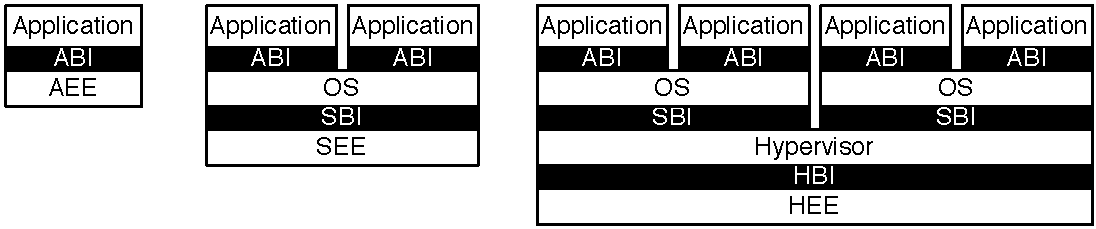
\includegraphics[width=\textwidth]{figs/privimps.pdf}
\caption{Different implementation stacks supporting various forms of
  privileged execution.}
\label{fig:privimps}
\end{figure}

\begin{commentary}
Our graphical convention represents abstract interfaces using black
boxes with white text, to separate them from concrete instances of
components implementing the interfaces.
\end{commentary}

The middle configuration shows a conventional operating system (OS)
that can support multiprogrammed execution of multiple
applications. Each application communicates over an ABI with the OS,
which provides the AEE.  Just as applications interface with an AEE
via an ABI, RISC-V operating systems interface with a supervisor
execution environment (SEE) via a supervisor binary interface (SBI).
An SBI comprises the user-level and supervisor-level ISA together with
a set of SBI function calls.  Using a single SBI across all SEE
implementations allows a single OS binary image to run on any SEE.
The SEE can be a simple boot loader and BIOS-style IO system in a
low-end hardware platform, or a hypervisor-provided virtual machine in
a high-end server, or a thin translation layer over a host operating
system in an architecture simulation environment.

\begin{commentary}
Most supervisor-level ISA definitions do not separate the SBI from the
execution environment and/or the hardware platform, complicating
virtualization and bring-up of new hardware platforms.
\end{commentary}

The rightmost configuration shows a virtual machine monitor
configuration where multiple multiprogrammed OSs are supported by a
single hypervisor.  Each OS communicates via an SBI with the
hypervisor, which provides the SEE.  The hypervisor communicates with
the hypervisor execution environment (HEE) using a hypervisor binary
interface (HBI), to isolate the hypervisor from details of the
hardware platform.

\begin{commentary}
The ABI, SBI, and HBI are still a work-in-progress, but we are now
prioritizing support for Type-2 hypervisors where the SBI is provided
recursively by an S-mode OS.
\end{commentary}

Hardware implementations of the RISC-V ISA will generally require
additional features beyond the privileged ISA to support the various
execution environments (AEE, SEE, or HEE).

\section{Privilege Levels}

At any time, a RISC-V hardware thread ({\em hart}) is running at some
privilege level encoded as a mode in one or more CSRs (control and
status registers).  Three RISC-V privilege levels are currently defined
as shown in Table~\ref{privlevels}.

\begin{table*}[h!]
\begin{center}
\begin{tabular}{|c|c|c|c|}
  \hline
   Level & Encoding & Name      & Abbreviation \\ \hline  
   0     & \tt 00   & User/Application & U     \\ 
   1     & \tt 01   & Supervisor & S           \\ 
   2     & \tt 10   & {\em Reserved} &            \\ 
   3     & \tt 11   & Machine    & M           \\ 
  \hline
 \end{tabular}
\end{center}
\caption{RISC-V privilege levels.}
\label{privlevels}
\end{table*}

Privilege levels are used to provide protection between different
components of the software stack, and attempts to perform operations
not permitted by the current privilege mode will cause an exception to
be raised.  These exceptions will normally cause traps into an
underlying execution environment.

\begin{commentary}
In the description, we try to separate the {\em privilege level} for
which code is written, from the {\em privilege mode} in which it runs,
although the two are often tied.  For example, a supervisor-level
operating system can run in supervisor-mode on a system with three
privilege modes, but can also run in user-mode under a classic virtual
machine monitor on systems with two or more privilege modes.  In both
cases, the same supervisor-level operating system binary code can be
used, coded to a supervisor-level SBI and hence expecting to be able
to use supervisor-level privileged instructions and CSRs.  When
running a guest OS in user mode, all supervisor-level actions will be
trapped and emulated by the SEE running in the higher-privilege level.
\end{commentary}

The machine level has the highest privileges and is the only mandatory
privilege level for a RISC-V hardware platform.  Code run in
machine-mode (M-mode) is usually inherently trusted, as it has
low-level access to the machine implementation.  M-mode can be used to
manage secure execution environments on RISC-V.  User-mode (U-mode)
and supervisor-mode (S-mode) are intended for conventional application
and operating system usage respectively.

\begin{commentary}
The previous Hypervisor mode (H-mode) designed to support Type-1
hypervisors has been removed and the encoding space reserved as we are
focusing on hypervisor support via an extended S mode suitable for
both Type-1 and Type-2 hypervisors as described in
Chapter~\ref{hypervisor}.  The encoding space for H is reserved for
future use and to avoid backwards incompatible changes in bit
positions in various status registers.  The bit positions might be
reused in the future for different Type-1 hypervisor support or
possibly additional secure execution modes.
\end{commentary}

Each privilege level has a core set of privileged ISA extensions with optional
extensions and variants.  For example, machine-mode supports an optional
standard extension for memory protection.  Also, supervisor mode can be
extended to support Type-2 hypervisor execution as described in
Chapter~\ref{hypervisor}.

Implementations might provide anywhere from 1 to 3 privilege modes
trading off reduced isolation for lower implementation cost, as shown
in Table~\ref{privcombs}.

\begin{table*}[h!]
\begin{center}
\begin{tabular}{|c|l|l|}
  \hline
   Number of levels &  Supported Modes & Intended Usage \\ \hline  
   1     & M          & Simple embedded systems \\ 
   2     & M, U       & Secure embedded systems \\ 
   3     & M, S, U    & Systems running Unix-like operating systems\\ 
  \hline
 \end{tabular}
\end{center}
\caption{Supported combinations of privilege modes.}
\label{privcombs}
\end{table*}

All hardware implementations must provide M-mode, as this is the only
mode that has unfettered access to the whole machine.  The simplest
RISC-V implementations may provide only M-mode, though this will
provide no protection against incorrect or malicious application code.

\begin{commentary}
  The lock feature of the optional PMP facility can provide some
  limited protection even with only M-mode implemented.
\end{commentary}

Many RISC-V implementations will also support at least user mode
(U-mode) to protect the rest of the system from application code.
Supervisor mode (S-mode) can be added to provide isolation between a
supervisor-level operating system and the SEE.

A hart normally runs application code in U-mode until some trap (e.g.,
a supervisor call or a timer interrupt) forces a switch to a trap
handler, which usually runs in a more privileged mode. The hart will
then execute the trap handler, which will eventually resume execution
at or after the original trapped instruction in U-mode.  Traps that
increase privilege level are termed {\em vertical} traps, while traps
that remain at the same privilege level are termed {\em horizontal}
traps.  The RISC-V privileged architecture provides flexible routing
of traps to different privilege layers.

\begin{commentary}
Horizontal traps can be implemented as vertical traps that
return control to a horizontal trap handler in the less-privileged mode.
\end{commentary}

\section{Debug Mode}

Implementations may also include a debug mode to support off-chip
debugging and/or manufacturing test.  Debug mode (D-mode) can be
considered an additional privilege mode, with even more access than
M-mode. The separate debug specification proposal describes operation
of a RISC-V hart in debug mode.  Debug mode reserves a few CSR
addresses that are only accessible in D-mode, and may also reserve
some portions of the physical memory space on a platform.

\chapter{Control and Status Registers (CSRs)}
\label{chap:priv-csrs}

The SYSTEM major opcode is used to encode all privileged instructions
in the RISC-V ISA.  These can be divided into two main classes: those
that atomically read-modify-write control and status registers (CSRs),
and all other privileged instructions.  In addition to the user-level
state described in Volume I of this manual, an implementation may
contain additional CSRs, accessible by some subset of the privilege
levels using the CSR instructions described in the user-level manual.
In this chapter, we map out the CSR address space.  The following
chapters describe the function of each of the CSRs according to
privilege level, as well as the other privileged instructions which
are generally closely associated with a particular privilege level.
Note that although CSRs and instructions are associated with one
privilege level, they are also accessible at all higher privilege
levels.

\section{CSR Address Mapping Conventions}

The standard RISC-V ISA sets aside a 12-bit encoding space (csr[11:0])
for up to 4,096 CSRs.  By convention, the upper 4 bits of the CSR
address (csr[11:8]) are used to encode the read and write
accessibility of the CSRs according to privilege level as shown in
Table~\ref{csrrwpriv}.  The top two bits (csr[11:10]) indicate whether
the register is read/write ({\tt 00}, {\tt 01}, or {\tt 10}) or
read-only ({\tt 11}).  The next two bits (csr[9:8]) encode the lowest
privilege level that can access the CSR.

\begin{commentary}
The CSR address convention uses the upper bits of the CSR address to
encode default access privileges.  This simplifies error checking in
the hardware and provides a larger CSR space, but does constrain the
mapping of CSRs into the address space.

Implementations might allow a more-privileged level to trap otherwise
permitted CSR accesses by a less-privileged level to allow these
accesses to be intercepted.  This change should be transparent to the
less-privileged software.
\end{commentary}

\begin{table*}[h!]
\begin{center}
\begin{tabular}{|c|c|c|c|l|}
\hline
\multicolumn{3}{|c|}{CSR Address} & Hex & \multicolumn{1}{c|}{Use and Accessibility}\\ \cline{1-3}
[11:10] & [9:8] & [7:4]                  &  & \\
\hline
\multicolumn{5}{|c|}{User CSRs}  \\
\hline
\tt   00   &\tt   00  &\tt   XXXX   & \tt 0x000-0x0FF & Standard read/write \\
\tt   01   &\tt   00  &\tt   XXXX   & \tt 0x400-0x4FF & Standard read/write \\
\tt   10   &\tt   00  &\tt   XXXX   & \tt 0x800-0x8FF & Custom read/write \\
\tt   11   &\tt   00  &\tt   0XXX   & \tt 0xC00-0xC7F & Standard read-only \\
\tt   11   &\tt   00  &\tt   10XX   & \tt 0xC80-0xCBF & Standard read-only \\
\tt   11   &\tt   00  &\tt   11XX   & \tt 0xCC0-0xCFF & Custom read-only \\
\hline
\multicolumn{5}{|c|}{Supervisor CSRs}  \\
\hline
\tt   00   &\tt   01  &\tt   XXXX   & \tt 0x100-0x1FF & Standard read/write \\
\tt   01   &\tt   01  &\tt   0XXX   & \tt 0x500-0x57F & Standard read/write \\
\tt   01   &\tt   01  &\tt   10XX   & \tt 0x580-0x5BF & Standard read/write \\
\tt   01   &\tt   01  &\tt   11XX   & \tt 0x5C0-0x5FF & Custom read/write \\
\tt   10   &\tt   01  &\tt   0XXX   & \tt 0x900-0x97F & Standard read/write \\
\tt   10   &\tt   01  &\tt   10XX   & \tt 0x980-0x9BF & Standard read/write \\
\tt   10   &\tt   01  &\tt   11XX   & \tt 0x9C0-0x9FF & Custom read/write \\
\tt   11   &\tt   01  &\tt   0XXX   & \tt 0xD00-0xD7F & Standard read-only \\
\tt   11   &\tt   01  &\tt   10XX   & \tt 0xD80-0xDBF & Standard read-only \\
\tt   11   &\tt   01  &\tt   11XX   & \tt 0xDC0-0xDFF & Custom read-only \\
\hline
\multicolumn{5}{|c|}{Hypervisor CSRs} \\
\hline
\tt   00   &\tt   10  &\tt   XXXX   & \tt 0x200-0x2FF & Standard read/write \\
\tt   01   &\tt   10  &\tt   0XXX   & \tt 0x600-0x67F & Standard read/write \\
\tt   01   &\tt   10  &\tt   10XX   & \tt 0x680-0x6BF & Standard read/write \\
\tt   01   &\tt   10  &\tt   11XX   & \tt 0x6C0-0x6FF & Custom read/write \\
\tt   10   &\tt   10  &\tt   0XXX   & \tt 0xA00-0xA7F & Standard read/write \\
\tt   10   &\tt   10  &\tt   10XX   & \tt 0xA80-0xABF & Standard read/write \\
\tt   10   &\tt   10  &\tt   11XX   & \tt 0xAC0-0xAFF & Custom read/write \\
\tt   11   &\tt   10  &\tt   0XXX   & \tt 0xE00-0xE7F & Standard read-only \\
\tt   11   &\tt   10  &\tt   10XX   & \tt 0xE80-0xEBF & Standard read-only \\
\tt   11   &\tt   10  &\tt   11XX   & \tt 0xEC0-0xEFF & Custom read-only \\
\hline
\multicolumn{5}{|c|}{Machine CSRs}  \\
\hline
\tt   00   &\tt   11  &\tt   XXXX   & \tt 0x300-0x3FF & Standard read/write \\
\tt   01   &\tt   11  &\tt   0XXX   & \tt 0x700-0x77F & Standard read/write \\
\tt   01   &\tt   11  &\tt   100X   & \tt 0x780-0x79F & Standard read/write \\
\tt   01   &\tt   11  &\tt   1010   & \tt 0x7A0-0x7AF & Standard read/write debug CSRs  \\
\tt   01   &\tt   11  &\tt   1011   & \tt 0x7B0-0x7BF & Debug-mode-only CSRs \\
\tt   01   &\tt   11  &\tt   11XX   & \tt 0x7C0-0x7FF & Custom read/write \\
\tt   10   &\tt   11  &\tt   0XXX   & \tt 0xB00-0xB7F & Standard read/write \\
\tt   10   &\tt   11  &\tt   10XX   & \tt 0xB80-0xBBF & Standard read/write \\
\tt   10   &\tt   11  &\tt   11XX   & \tt 0xBC0-0xBFF & Custom read/write \\
\tt   11   &\tt   11  &\tt   0XXX   & \tt 0xF00-0xF7F & Standard read-only \\
\tt   11   &\tt   11  &\tt   10XX   & \tt 0xF80-0xFBF & Standard read-only \\
\tt   11   &\tt   11  &\tt   11XX   & \tt 0xFC0-0xFFF & Custom read-only \\
\hline
\end{tabular}
\end{center}
\caption{Allocation of RISC-V CSR address ranges.}
\label{csrrwpriv}
\end{table*}

Attempts to access a non-existent CSR raise an illegal instruction
exception.  Attempts to access a CSR without appropriate privilege
level or to write a read-only register also raise illegal instruction
exceptions.  A read/write register might also contain some bits that
are read-only, in which case writes to the read-only bits are ignored.

Table~\ref{csrrwpriv} also indicates the convention to allocate CSR
addresses between standard and custom uses.  The CSR addresses
reserved for custom uses will not be redefined by future
standard extensions.

Machine-mode standard read-write CSRs {\tt 0x7A0}--{\tt 0x7BF} are reserved
for use by the debug system.  Of these CSRs, {\tt 0x7A0}--{\tt 0x7AF} are
accessible to machine mode, whereas {\tt 0x7B0}--{\tt 0x7BF} are only visible
to debug mode.  Implementations should raise illegal instruction exceptions on
machine-mode access to the latter set of registers.

\begin{commentary}
Effective virtualization requires that as many instructions run natively as
possible inside a virtualized environment, while any privileged accesses trap
to the virtual machine monitor~\cite{goldbergvm}.  CSRs that are read-only at
some lower privilege level are shadowed into separate CSR addresses if they
are made read-write at a higher privilege level.  This avoids trapping
permitted lower-privilege accesses while still causing traps on illegal
accesses.  Currently, the counters are the only shadowed CSRs.
\end{commentary}

\section{CSR Listing}

Tables~\ref{ucsrnames}--\ref{mcsrnames1} list the CSRs that have
currently been allocated CSR addresses.  The timers, counters, and
floating-point CSRs are standard user-level CSRs, as well as the
additional user trap registers added by the N extension.  The other
registers are used by privileged code, as described in the following
chapters.  Note that not all registers are required on all
implementations.

\begin{table}[htb!]
\begin{center}
\begin{tabular}{|l|l|l|l|}
\hline
Number    & Privilege & Name & Description \\
\hline
\multicolumn{4}{|c|}{User Trap Setup} \\
\hline
\tt 0x000 & URW  &\tt ustatus    & User status register. \\
\tt 0x004 & URW  &\tt uie        & User interrupt-enable register. \\
\tt 0x005 & URW  &\tt utvec      & User trap handler base address. \\
\hline
\multicolumn{4}{|c|}{User Trap Handling} \\
\hline
\tt 0x040 & URW  &\tt uscratch   & Scratch register for user trap handlers. \\
\tt 0x041 & URW  &\tt uepc       & User exception program counter. \\
\tt 0x042 & URW  &\tt ucause     & User trap cause. \\
\tt 0x043 & URW  &\tt utval      & User bad address or instruction. \\
\tt 0x044 & URW  &\tt uip        & User interrupt pending. \\
\hline
\multicolumn{4}{|c|}{User Floating-Point CSRs} \\
\hline
\tt 0x001 & URW  &\tt fflags     & Floating-Point Accrued Exceptions. \\
\tt 0x002 & URW  &\tt frm        & Floating-Point Dynamic Rounding Mode. \\
\tt 0x003 & URW  &\tt fcsr       & Floating-Point Control and Status
Register ({\tt frm} + {\tt fflags}). \\
\hline
\multicolumn{4}{|c|}{User Counter/Timers} \\
\hline
\tt 0xC00 & URO  &\tt cycle         & Cycle counter for RDCYCLE instruction. \\
\tt 0xC01 & URO  &\tt time          & Timer for RDTIME instruction. \\
\tt 0xC02 & URO  &\tt instret       & Instructions-retired counter for RDINSTRET instruction. \\
\tt 0xC03 & URO  &\tt hpmcounter3   & Performance-monitoring counter. \\
\tt 0xC04 & URO  &\tt hpmcounter4   & Performance-monitoring counter. \\
& & \multicolumn{1}{c|}{\vdots} & \ \\
\tt 0xC1F & URO  &\tt hpmcounter31  & Performance-monitoring counter. \\
\tt 0xC80 & URO  &\tt cycleh        & Upper 32 bits of {\tt cycle}, RV32 only. \\
\tt 0xC81 & URO  &\tt timeh         & Upper 32 bits of {\tt time}, RV32 only. \\
\tt 0xC82 & URO  &\tt instreth      & Upper 32 bits of {\tt instret}, RV32 only. \\
\tt 0xC83 & URO  &\tt hpmcounter3h  & Upper 32 bits of {\tt hpmcounter3}, RV32 only. \\
\tt 0xC84 & URO  &\tt hpmcounter4h  & Upper 32 bits of {\tt hpmcounter4}, RV32 only. \\
& & \multicolumn{1}{c|}{\vdots} & \ \\
\tt 0xC9F & URO  &\tt hpmcounter31h & Upper 32 bits of {\tt hpmcounter31}, RV32 only. \\
\hline
\end{tabular}
\end{center}
\caption{Currently allocated RISC-V user-level CSR addresses.}
\label{ucsrnames}
\end{table}

\begin{table}[htb!]
\begin{center}
\begin{tabular}{|l|l|l|l|}
\hline
Number    & Privilege & Name & Description \\
\hline
\multicolumn{4}{|c|}{Supervisor Trap Setup} \\
\hline
\tt 0x100 & SRW  &\tt sstatus    & Supervisor status register. \\
\tt 0x102 & SRW  &\tt sedeleg    & Supervisor exception delegation register. \\
\tt 0x103 & SRW  &\tt sideleg    & Supervisor interrupt delegation register. \\
\tt 0x104 & SRW  &\tt sie        & Supervisor interrupt-enable register. \\
\tt 0x105 & SRW  &\tt stvec      & Supervisor trap handler base address. \\
\tt 0x106 & SRW  &\tt scounteren & Supervisor counter enable. \\
\hline
\multicolumn{4}{|c|}{Supervisor Trap Handling} \\
\hline
\tt 0x140 & SRW  &\tt sscratch   & Scratch register for supervisor trap handlers. \\
\tt 0x141 & SRW  &\tt sepc       & Supervisor exception program counter. \\
\tt 0x142 & SRW  &\tt scause     & Supervisor trap cause. \\
\tt 0x143 & SRW  &\tt stval      & Supervisor bad address or instruction. \\
\tt 0x144 & SRW  &\tt sip        & Supervisor interrupt pending. \\
\hline
\multicolumn{4}{|c|}{Supervisor Protection and Translation} \\
\hline
\tt 0x180 & SRW  &\tt satp       & Supervisor address translation and protection. \\
\hline
\end{tabular}
\end{center}
\caption{Currently allocated RISC-V supervisor-level CSR addresses.}
\label{scsrnames}
\end{table}

\begin{table}[htb!]
\begin{center}
\begin{tabular}{|l|l|l|l|}
\hline
Number    & Privilege & Name & Description \\
\hline
\multicolumn{4}{|c|}{Hypervisor Trap Setup} \\
\hline
\hline
\tt 0x600 & HRW  &\tt hstatus    & Hypervisor status register. \\
\tt 0x602 & HRW  &\tt hedeleg    & Hypervisor exception delegation register. \\
\tt 0x603 & HRW  &\tt hideleg    & Hypervisor interrupt delegation register. \\
\tt 0x604 & HRW  &\tt hie        & Hypervisor interrupt-enable register. \\
\tt 0x606 & HRW  &\tt hcounteren & Hypervisor counter enable. \\
\hline
\multicolumn{4}{|c|}{Hypervisor Trap Handling} \\
\hline
\tt 0x643 & HRW  &\tt htval      & Hypervisor bad guest physical address. \\
\tt 0x644 & HRW  &\tt hip        & Hypervisor interrupt pending. \\
\tt 0x64A & HRW  &\tt htinst     & Hypervisor trap instruction (transformed). \\
\hline
\multicolumn{4}{|c|}{Hypervisor Protection and Translation} \\
\hline
\tt 0x680 & HRW  &\tt hgatp      & Hypervisor guest address translation and protection. \\
\hline
\multicolumn{4}{|c|}{Hypervisor Counter/Timer Virtualization Registers} \\
\hline
\tt 0x605 & HRW  &\tt htimedelta   & Delta for VS/VU-mode timer. \\
\tt 0x615 & HRW  &\tt htimedeltah  & Upper 32 bits of {\tt htimedelta}, RV32 only. \\
\hline
\multicolumn{4}{|c|}{Virtual Supervisor Registers} \\
\hline
\tt 0x200 & HRW  &\tt vsstatus   & Virtual supervisor status register. \\
\tt 0x204 & HRW  &\tt vsie       & Virtual supervisor interrupt-enable register. \\
\tt 0x205 & HRW  &\tt vstvec     & Virtual supervisor trap handler base address. \\
\tt 0x240 & HRW  &\tt vsscratch  & Virtual supervisor scratch register. \\
\tt 0x241 & HRW  &\tt vsepc      & Virtual supervisor exception program counter. \\
\tt 0x242 & HRW  &\tt vscause    & Virtual supervisor trap cause. \\
\tt 0x243 & HRW  &\tt vstval     & Virtual supervisor bad address or instruction. \\
\tt 0x244 & HRW  &\tt vsip       & Virtual supervisor interrupt pending. \\
\tt 0x280 & HRW  &\tt vsatp      & Virtual supervisor address translation and protection. \\
\hline
\end{tabular}
\end{center}
\caption{Currently allocated RISC-V hypervisor-level CSR addresses.}
\label{hcsrnames}
\end{table}


\begin{table}[htb!]
\begin{center}
\begin{tabular}{|l|l|l|l|}
\hline
Number    & Privilege & Name & Description \\
\hline
\multicolumn{4}{|c|}{Machine Information Registers} \\
\hline
\tt 0xF11 & MRO &\tt mvendorid   & Vendor ID. \\
\tt 0xF12 & MRO &\tt marchid     & Architecture ID. \\
\tt 0xF13 & MRO &\tt mimpid      & Implementation ID. \\
\tt 0xF14 & MRO &\tt mhartid     & Hardware thread ID. \\
\hline
\multicolumn{4}{|c|}{Machine Trap Setup} \\
\hline
\tt 0x300 & MRW  &\tt mstatus    & Machine status register. \\
\tt 0x301 & MRW  &\tt misa       & ISA and extensions \\
\tt 0x302 & MRW  &\tt medeleg    & Machine exception delegation register. \\
\tt 0x303 & MRW  &\tt mideleg    & Machine interrupt delegation register. \\
\tt 0x304 & MRW  &\tt mie        & Machine interrupt-enable register. \\
\tt 0x305 & MRW  &\tt mtvec      & Machine trap-handler base address. \\
\tt 0x306 & MRW  &\tt mcounteren & Machine counter enable. \\
\tt 0x310 & MRW  &\tt mstatush   & Additional machine status register, RV32 only. \\
\hline
\multicolumn{4}{|c|}{Machine Trap Handling} \\
\hline
\tt 0x340 & MRW  &\tt mscratch   & Scratch register for machine trap handlers. \\
\tt 0x341 & MRW  &\tt mepc       & Machine exception program counter. \\
\tt 0x342 & MRW  &\tt mcause     & Machine trap cause. \\
\tt 0x343 & MRW  &\tt mtval      & Machine bad address or instruction. \\
\tt 0x344 & MRW  &\tt mip        & Machine interrupt pending. \\
\tt 0x34A & MRW  &\tt mtinst     & Machine trap instruction (transformed). \\
\tt 0x34B & MRW  &\tt mtval2     & Machine bad guest physical address. \\
\hline
\multicolumn{4}{|c|}{Machine Memory Protection} \\
\hline
%\tt 0x380 & MRW  &\tt mbase      & Base register. \\
%\tt 0x381 & MRW  &\tt mbound     & Bound register. \\
%\tt 0x382 & MRW  &\tt mibase     & Instruction base register. \\
%\tt 0x383 & MRW  &\tt mibound    & Instruction bound register. \\
%\tt 0x384 & MRW  &\tt mdbase     & Data base register. \\
%\tt 0x385 & MRW  &\tt mdbound    & Data bound register. \\
\tt 0x3A0 & MRW  &\tt pmpcfg0    & Physical memory protection configuration. \\
\tt 0x3A1 & MRW  &\tt pmpcfg1    & Physical memory protection configuration, RV32 only. \\
\tt 0x3A2 & MRW  &\tt pmpcfg2    & Physical memory protection configuration. \\
\tt 0x3A3 & MRW  &\tt pmpcfg3    & Physical memory protection configuration, RV32 only. \\
\tt 0x3B0 & MRW  &\tt pmpaddr0   & Physical memory protection address register. \\
\tt 0x3B1 & MRW  &\tt pmpaddr1   & Physical memory protection address register. \\
& & \multicolumn{1}{c|}{\vdots} & \ \\
\tt 0x3BF & MRW  &\tt pmpaddr15  & Physical memory protection address register. \\
\hline
\end{tabular}
\end{center}
\caption{Currently allocated RISC-V machine-level CSR addresses.}
\label{mcsrnames0}
\end{table}

\begin{table}[htb!]
\begin{center}
\begin{tabular}{|l|l|l|l|}
\hline
Number    & Privilege & Name & Description \\
\hline
\multicolumn{4}{|c|}{Machine Counter/Timers} \\
\hline
\tt 0xB00 & MRW  &\tt mcycle         & Machine cycle counter. \\
\tt 0xB02 & MRW  &\tt minstret       & Machine instructions-retired counter. \\
\tt 0xB03 & MRW  &\tt mhpmcounter3   & Machine performance-monitoring counter. \\
\tt 0xB04 & MRW  &\tt mhpmcounter4   & Machine performance-monitoring counter. \\
& & \multicolumn{1}{c|}{\vdots} & \ \\
\tt 0xB1F & MRW  &\tt mhpmcounter31  & Machine performance-monitoring counter. \\
\tt 0xB80 & MRW  &\tt mcycleh        & Upper 32 bits of {\tt mcycle}, RV32 only. \\
\tt 0xB82 & MRW  &\tt minstreth      & Upper 32 bits of {\tt minstret}, RV32 only. \\
\tt 0xB83 & MRW  &\tt mhpmcounter3h  & Upper 32 bits of {\tt mhpmcounter3}, RV32 only. \\
\tt 0xB84 & MRW  &\tt mhpmcounter4h  & Upper 32 bits of {\tt mhpmcounter4}, RV32 only. \\
& & \multicolumn{1}{c|}{\vdots} & \ \\
\tt 0xB9F & MRW  &\tt mhpmcounter31h & Upper 32 bits of {\tt mhpmcounter31}, RV32 only. \\
\hline
\multicolumn{4}{|c|}{Machine Counter Setup} \\
\hline
\tt 0x320 & MRW  &\tt mcountinhibit  & Machine counter-inhibit register. \\
\tt 0x323 & MRW  &\tt mhpmevent3     & Machine performance-monitoring event selector. \\
\tt 0x324 & MRW  &\tt mhpmevent4     & Machine performance-monitoring event selector. \\
& & \multicolumn{1}{c|}{\vdots} & \ \\
\tt 0x33F & MRW  &\tt mhpmevent31    & Machine performance-monitoring event selector. \\
\hline
\multicolumn{4}{|c|}{Debug/Trace Registers (shared with Debug Mode)} \\
\hline
\tt 0x7A0 & MRW &\tt tselect & Debug/Trace trigger register select. \\
\tt 0x7A1 & MRW &\tt tdata1 & First Debug/Trace trigger data register. \\
\tt 0x7A2 & MRW &\tt tdata2 & Second Debug/Trace trigger data register. \\
\tt 0x7A3 & MRW &\tt tdata3 & Third Debug/Trace trigger data register. \\
\hline
\multicolumn{4}{|c|}{Debug Mode Registers } \\
\hline
\tt 0x7B0 & DRW &\tt dcsr & Debug control and status register. \\
\tt 0x7B1 & DRW &\tt dpc & Debug PC. \\
\tt 0x7B2 & DRW &\tt dscratch0 & Debug scratch register 0. \\
\tt 0x7B3 & DRW &\tt dscratch1 & Debug scratch register 1. \\
\hline
\end{tabular}
\end{center}
\caption{Currently allocated RISC-V machine-level CSR addresses.}
\label{mcsrnames1}
\end{table}

\clearpage

\section{CSR Field Specifications}


The following definitions and abbreviations are used in specifying the
behavior of fields within the CSRs.

\subsection*{Reserved Writes Preserve Values, Reads Ignore Values (WPRI)}

Some whole read/write fields are reserved for future use.  Software
should ignore the values read from these fields, and should preserve
the values held in these fields when writing values to other fields of
the same register.
For forward compatibility, implementations that do not furnish these fields
must hardwire them to zero.
These fields are labeled \wpri\ in the register descriptions.

\begin{commentary}
To simplify the software model, any backward-compatible future
definition of previously reserved fields within a CSR must cope with
the possibility that a non-atomic read/modify/write sequence is used
to update other fields in the CSR.  Alternatively, the original CSR
definition must specify that subfields can only be updated atomically,
which may require a two-instruction clear bit/set bit sequence in
general that can be problematic if intermediate values are not legal.
\end{commentary}

\subsection*{Write/Read Only Legal Values (WLRL)}

Some read/write CSR fields specify behavior for only a subset of
possible bit encodings, with other bit encodings reserved.  Software
should not write anything other than legal values to such a field, and
should not assume a read will return a legal value unless the last
write was of a legal value, or the register has not been written since
another operation (e.g., reset) set the register to a legal value.
These fields are labeled \wlrl\ in the register descriptions.

\begin{commentary}
Hardware implementations need only implement enough state bits to
differentiate between the supported values, but must always return the
complete specified bit-encoding of any supported value when read.
\end{commentary}

Implementations are permitted but not required to raise an illegal
instruction exception if an instruction attempts to write a
non-supported value to a \wlrl\ field.  Implementations can
return arbitrary bit patterns on the read of a \wlrl\ field when the last
write was of an illegal value, but the value returned should
deterministically depend on the illegal written value and
the value of the field prior to the write.

\subsection*{Write Any Values, Reads Legal Values (WARL)}

Some read/write CSR fields are only defined for a subset of bit
encodings, but allow any value to be written while guaranteeing to
return a legal value whenever read.  Assuming that writing the CSR has
no other side effects, the range of supported values can be determined
by attempting to write a desired setting then reading to see if the
value was retained.  These fields are labeled \warl\ in the register
descriptions.

Implementations will not raise an exception on writes of unsupported
values to a \warl\ field.  Implementations can
return any legal value on the read of a \warl\ field when the last
write was of an illegal value, but the legal value returned should
deterministically depend on the illegal written value and
the value of the field prior to the write.

\section{CSR Width Modulation}
\label{sec:csrwidthmodulation}

If the width of a CSR is changed (for example, by changing MXLEN or UXLEN, as
described in Section~\ref{xlen-control}), the values of the {\em writable}
fields and bits of the new-width CSR are, unless specified otherwise,
determined from the previous-width CSR as though by this algorithm:

\begin{enumerate}

\item The value of the previous-width CSR is copied to a temporary register of
the same width.

\item For the read-only bits of the previous-width CSR, the bits at the same
positions in the temporary register are set to zeros.

\item The width of the temporary register is changed to the new width. If the
new width $W$ is narrower than the previous width, the least-significant $W$
bits of the temporary register are retained and the more-significant bits are
discarded. If the new width is wider than the previous width, the temporary
register is zero-extended to the wider width.

\item Each writable field of the new-width CSR takes the value of the bits at
the same positions in the temporary register.

\end{enumerate}

Changing the width of a CSR is not a read or write of the CSR and thus
does not trigger any side effects.

\chapter{Machine-Level ISA, Version 1.12}
\label{machine}

This chapter describes the machine-level operations available in
machine-mode (M-mode), which is the highest privilege mode in a RISC-V
system.  M-mode is used for low-level access to a
hardware platform and is the first mode entered at reset.  M-mode can
also be used to implement features that are too difficult or expensive
to implement in hardware directly.  The RISC-V machine-level ISA
contains a common core that is extended depending on which other
privilege levels are supported and other details of the hardware
implementation.

\section{Machine-Level CSRs}

In addition to the machine-level CSRs described in this section,
M-mode code can access all CSRs at lower privilege levels.

\subsection{Machine ISA Register {\tt misa}}
\label{sec:misa}

The {\tt misa} CSR is a \warl\ read-write register
reporting the ISA supported by the hart.  This register must be
readable in any implementation, but a value of zero can be returned to
indicate the {\tt misa} register has not been implemented, requiring
that CPU capabilities be determined through a separate non-standard
mechanism.

\begin{figure*}[h!]
{\footnotesize
\begin{center}
\begin{tabular}{c@{}c@{}L}
\instbitrange{MXLEN-1}{MXLEN-2} &
\instbitrange{MXLEN-3}{26} &
\instbitrange{25}{0} \\
\hline
\multicolumn{1}{|c|}{MXL[1:0] (\warl)} &
\multicolumn{1}{c|}{\wlrl} &
\multicolumn{1}{c|}{Extensions[25:0] (\warl)} \\
\hline
2 & MXLEN-28 & 26 \\
\end{tabular}
\end{center}
}
\vspace{-0.1in}
\caption{Machine ISA register ({\tt misa}).}
\label{misareg}
\end{figure*}

The MXL (Machine XLEN) field encodes the native base integer ISA width
as shown in Table~\ref{misabase}.  The MXL field may be writable in
implementations that support multiple base ISA widths.  The effective
XLEN in M-mode, {\em MXLEN}, is given by the setting of MXL, or has a
fixed value if {\tt misa} is zero.  The MXL field is always set to the
widest supported ISA variant at reset.

\begin{table*}[h!]
\begin{center}
\begin{tabular}{|r|r|}
\hline
MXL  & XLEN \\
\hline	 
1   & 32 \\
2   & 64 \\
3   & 128 \\
\hline
\end{tabular}
\end{center}
\caption{Encoding of MXL field in {\tt misa}}
\label{misabase}
\end{table*}

The {\tt misa} CSR is MXLEN bits wide.  If the value read from {\tt misa} is
nonzero, field MXL of that value always denotes the current MXLEN. If a write
to {\tt misa} causes MXLEN to change, the position of MXL moves to the
most-significant two bits of {\tt misa} at the new width.

\begin{commentary}
The base width can be quickly ascertained using branches on the sign
of the returned {\tt misa} value, and possibly a shift left by one and
a second branch on the sign.  These checks can be written in assembly
code without knowing the register width (XLEN) of the machine.  The
base width is given by $\mbox{XLEN}=2^{\mbox{MXL+4}}$.

The base width can also be found if {\tt misa} is zero, by placing the
immediate 4 in a register then shifting the register left by 31 bits
at a time.  If zero after one shift, then the machine is RV32.  If
zero after two shifts, then the machine is RV64, else RV128.
\end{commentary}

The Extensions field encodes the presence of the standard extensions,
with a single bit per letter of the alphabet (bit 0 encodes presence
of extension ``A'' , bit 1 encodes presence of extension ``B'',
through to bit 25 which encodes ``Z'').  The ``I'' bit will be set for
RV32I, RV64I, RV128I base ISAs, and the ``E'' bit will be set for
RV32E.  The Extensions field is a \warl\ field that can contain writable bits
where the implementation allows the supported ISA to be modified.  At
reset, the Extensions field should contain the maximal set of supported
extensions, and I should be selected over E if both are available.

The RV128I base ISA is not yet frozen, and while much of the remainder of this
specification is expected to apply to RV128, this version of the document
focuses only on RV32 and RV64.

The ``G'' bit is used as an escape to allow expansion to a larger
space of standard extension names.
\begin{commentary}
G is used to indicate the combination IMAFD, so is redundant in the
{\tt misa} CSR, hence we reserve the bit to indicate that
additional standard extensions are present.
\end{commentary}

The ``U'' and ``S'' bits will be set if there is support for user and
supervisor modes respectively.

The ``X'' bit will be set if there are any non-standard extensions.

\begin{table*}
\begin{center}
\begin{tabular}{|r|r|l|}
\hline
Bit & Character  & Description \\
\hline	 
  0 & A & Atomic extension \\
  1 & B & {\em Tentatively reserved for Bit-Manipulation extension} \\
  2 & C & Compressed extension \\
  3 & D & Double-precision floating-point extension \\
  4 & E & RV32E base ISA \\
  5 & F & Single-precision floating-point extension \\
  6 & G & Additional standard extensions present \\
  7 & H & Hypervisor extension \\
  8 & I & RV32I/64I/128I base ISA \\
  9 & J & {\em Tentatively reserved for Dynamically Translated Languages extension} \\
 10 & K & {\em Reserved} \\
 11 & L & {\em Tentatively reserved for Decimal Floating-Point extension} \\
 12 & M & Integer Multiply/Divide extension \\
 13 & N & User-level interrupts supported \\
 14 & O & {\em Reserved} \\
 15 & P & {\em Tentatively reserved for Packed-SIMD extension} \\
 16 & Q & Quad-precision floating-point extension \\
 17 & R & {\em Reserved} \\
 18 & S & Supervisor mode implemented \\
 19 & T & {\em Tentatively reserved for Transactional Memory extension} \\
 20 & U & User mode implemented \\
 21 & V & {\em Tentatively reserved for Vector extension} \\
 22 & W & {\em Reserved} \\
 23 & X & Non-standard extensions present \\
 24 & Y & {\em Reserved} \\
 25 & Z & {\em Reserved} \\
\hline
\end{tabular}
\end{center}
\caption{Encoding of Extensions field in {\tt misa}.  All bits that are
  reserved for future use must return zero when read.}
\label{misaletters}
\end{table*}


\begin{commentary}
The {\tt misa} CSR exposes a rudimentary catalog of CPU features
to machine-mode code.  More extensive information can be obtained in
machine mode by probing other machine registers, and examining other
ROM storage in the system as part of the boot process.

We require that lower privilege levels execute environment calls
instead of reading CPU registers to determine features available at
each privilege level. This enables virtualization layers to alter the
ISA observed at any level, and supports a much richer command
interface without burdening hardware designs.
\end{commentary}

The ``E'' bit is read-only.  Unless {\tt misa} is hardwired to zero, the ``E''
bit always reads as the complement of the ``I'' bit.  An implementation that
supports both RV32E and RV32I can select RV32E by clearing the ``I'' bit.

If an ISA feature {\em x} depends on an ISA feature {\em y}, then attempting
to enable feature {\em x} but disable feature {\em y} results in both features
being disabled.  For example, setting ``F''=0 and ``D''=1 results in both
``F'' and ``D'' being cleared.

An implementation may impose additional constraints on the collective setting
of two or more {\tt misa} fields, in which case they function collectively as
a single \warl\ field.  An attempt to write an unsupported combination causes
those bits to be set to some supported combination.

Writing {\tt misa} may increase IALIGN, e.g., by disabling the ``C''
extension.
If an instruction that would write {\tt misa} increases IALIGN, and
the subsequent instruction's address is not IALIGN-bit aligned, the
write to {\tt misa} is suppressed, leaving {\tt misa} unchanged.

\subsection{Machine Vendor ID Register {\tt mvendorid}}

The {\tt mvendorid} CSR is a 32-bit read-only register providing
the JEDEC manufacturer ID of the provider of the core.  This register
must be readable in any implementation, but a value of 0 can be
returned to indicate the field is not implemented or that this is a
non-commercial implementation.

\begin{figure*}[h!]
{\footnotesize
\begin{center}
\begin{tabular}{JS}
\instbitrange{31}{7} &
\instbitrange{6}{0} \\
\hline
\multicolumn{1}{|c|}{Bank} &
\multicolumn{1}{c|}{Offset} \\
\hline
25 & 7 \\
\end{tabular}
\end{center}
}
\vspace{-0.1in}
\caption{Vendor ID register ({\tt mvendorid}).}
\label{mvendorreg}
\end{figure*}

JEDEC manufacturer IDs are ordinarily encoded as a sequence of one-byte
continuation codes {\tt 0x7f}, terminated by a one-byte ID not equal to
{\tt 0x7f}, with an odd parity bit in the most-significant bit of each byte.
{\tt mvendorid} encodes the number of one-byte continuation
codes in the Bank field, and encodes the final byte in the Offset field,
discarding the parity bit.  For example, the JEDEC manufacturer ID
{\tt 0x7f 0x7f 0x7f 0x7f 0x7f 0x7f 0x7f 0x7f 0x7f 0x7f 0x7f 0x7f 0x8a}
(twelve continuation codes followed by {\tt 0x8a}) would be encoded in the
{\tt mvendorid} field as {\tt 0x60a}.

\begin{commentary}
Previously the vendor ID was to be a number allocated by the RISC-V
Foundation, but this duplicates the work of JEDEC in maintaining a
manufacturer ID standard.  At time of writing, registering a
manufacturer ID with JEDEC has a one-time cost of \$500.
\end{commentary}

\subsection{Machine Architecture ID Register {\tt marchid}}

The {\tt marchid} CSR is an MXLEN-bit read-only register encoding the
base microarchitecture of the hart.  This register must be readable in
any implementation, but a value of 0 can be returned to indicate the
field is not implemented.  The combination of {\tt mvendorid} and {\tt
  marchid} should uniquely identify the type of hart microarchitecture
that is implemented.

\begin{figure*}[h!]
{\footnotesize
\begin{center}
\begin{tabular}{J}
\instbitrange{MXLEN-1}{0} \\
\hline
\multicolumn{1}{|c|}{Architecture ID} \\
\hline
MXLEN \\
\end{tabular}
\end{center}
}
\vspace{-0.1in}
\caption{Machine Architecture ID register ({\tt marchid}).}
\label{marchreg}
\end{figure*}

Open-source project architecture IDs are allocated globally by the
RISC-V Foundation, and have non-zero architecture IDs with a zero
most-significant-bit (MSB).  Commercial architecture IDs are allocated
by each commercial vendor independently, but must have the MSB set and
cannot contain zero in the remaining MXLEN-1 bits.

\begin{commentary}
The intent is for the architecture ID to represent the
microarchitecture associated with the repo around which development
occurs rather than a particular organization.  Commercial fabrications
of open-source designs should (and might be required by the license
to) retain the original architecture ID.  This will aid in reducing
fragmentation and tool support costs, as well as provide attribution.
Open-source architecture IDs should be administered by the Foundation
and should only be allocated to released, functioning open-source
projects.  Commercial architecture IDs can be managed independently by
any registered vendor but are required to have IDs disjoint from the
open-source architecture IDs (MSB set) to prevent collisions if a
vendor wishes to use both closed-source and open-source
microarchitectures.

The convention adopted within the following Implementation field can
be used to segregate branches of the same architecture design,
including by organization.  The {\tt misa} register also helps
distinguish different variants of a design.
\end{commentary}

\subsection{Machine Implementation ID Register {\tt mimpid}}

The {\tt mimpid} CSR provides a unique encoding of the version of the
processor implementation.  This register must be readable in any
implementation, but a value of 0 can be returned to indicate that the
field is not implemented.  The Implementation value should reflect the
design of the RISC-V processor itself and not any surrounding system.

\begin{figure*}[h!]
{\footnotesize
\begin{center}
\begin{tabular}{J}
\instbitrange{MXLEN-1}{0} \\
\hline
\multicolumn{1}{|c|}{Implementation}  \\
\hline
MXLEN \\
\end{tabular}
\end{center}
}
\vspace{-0.1in}
\caption{Machine Implementation ID register ({\tt mimpid}).}
\label{mimpidreg}
\end{figure*}

\begin{commentary}
The format of this field is left to the provider of the architecture
source code, but will often be printed by standard tools as a
hexadecimal string without any leading or trailing zeros, so the
Implementation value can be left-justified (i.e., filled in from
most-significant nibble down) with subfields aligned on nibble
boundaries to ease human readability.
\end{commentary}

\subsection{Hart ID Register {\tt mhartid}}

The {\tt mhartid} CSR is an MXLEN-bit read-only register
containing the integer ID of the hardware thread running the code.
This register must be readable in any implementation.  Hart IDs might
not necessarily be numbered contiguously in a multiprocessor system,
but at least one hart must have a hart ID of zero.  Hart IDs must be unique.

\begin{figure*}[h!]
{\footnotesize
\begin{center}
\begin{tabular}{J}
\instbitrange{MXLEN-1}{0} \\
\hline
\multicolumn{1}{|c|}{Hart ID}\\
\hline
MXLEN \\
\end{tabular}
\end{center}
}
\vspace{-0.1in}
\caption{Hart ID register ({\tt mhartid}).}
\label{mhartidreg}
\end{figure*}


\begin{commentary}
In certain cases, we must ensure exactly one hart runs some code
(e.g., at reset), and so require one hart to have a known hart ID of
zero.

For efficiency, system implementers should aim to reduce the magnitude
of the largest hart ID used in a system.
\end{commentary}

\subsection{Machine Status Registers ({\tt mstatus} and {\tt mstatush})}

The {\tt mstatus} register is an MXLEN-bit read/write register
formatted as shown in Figure~\ref{mstatusreg} for RV64 and
Figure~\ref{mstatusreg-rv32} for RV32.  The {\tt mstatus}
register keeps track of and controls the hart's current operating
state.  Restricted views of the {\tt mstatus} register appear as the
{\tt sstatus} and {\tt ustatus} registers in the S-level and U-level
ISAs respectively.

\begin{figure*}[h!]
{\footnotesize
\begin{center}
\setlength{\tabcolsep}{4pt}
\begin{tabular}{cRccccYcccccc}
\\
\instbit{MXLEN-1} &
\instbitrange{MXLEN-2}{38} &
\instbit{37} &
\instbit{36} &
\instbitrange{35}{34} &
\instbitrange{33}{32} &
\instbitrange{31}{23} &
\instbit{22} &
\instbit{21} &
\instbit{20} &
\instbit{19} &
\instbit{18} &
 \\
\hline
\multicolumn{1}{|c|}{SD} &
\multicolumn{1}{c|}{\wpri} &
\multicolumn{1}{c|}{MBE} &
\multicolumn{1}{c|}{SBE} &
\multicolumn{1}{c|}{SXL[1:0]} &
\multicolumn{1}{c|}{UXL[1:0]} &
\multicolumn{1}{c|}{\wpri} &
\multicolumn{1}{c|}{TSR} &
\multicolumn{1}{c|}{TW} &
\multicolumn{1}{c|}{TVM} &
\multicolumn{1}{c|}{MXR} &
\multicolumn{1}{c|}{SUM} &
 \\
\hline
1 & MXLEN-39 & 1 & 1 & 2 & 2 & 9 & 1 & 1 & 1 & 1 & 1 & \\
\end{tabular}
\begin{tabular}{ccccccccccccccc}
\\
&
\instbit{17} &
\instbitrange{16}{15} &
\instbitrange{14}{13} &
\instbitrange{12}{11} &
\instbitrange{10}{9} &
\instbit{8} &
\instbit{7} &
\instbit{6} &
\instbit{5} &
\instbit{4} &
\instbit{3} &
\instbit{2} &
\instbit{1} &
\instbit{0} \\
\hline
 &
\multicolumn{1}{|c|}{MPRV} &
\multicolumn{1}{c|}{XS[1:0]} &
\multicolumn{1}{c|}{FS[1:0]} &
\multicolumn{1}{c|}{MPP[1:0]} &
\multicolumn{1}{c|}{\wpri} &
\multicolumn{1}{c|}{SPP} &
\multicolumn{1}{c|}{MPIE} &
\multicolumn{1}{c|}{UBE} &
\multicolumn{1}{c|}{SPIE} &
\multicolumn{1}{c|}{UPIE} &
\multicolumn{1}{c|}{MIE} &
\multicolumn{1}{c|}{\wpri} &
\multicolumn{1}{c|}{SIE} &
\multicolumn{1}{c|}{UIE} \\
\hline
 & 1 & 2 & 2 & 2 & 2 & 1 & 1 & 1 & 1 & 1 & 1 & 1 & 1 & 1 \\
\end{tabular}
\end{center}
}
\vspace{-0.1in}
\caption{Machine-mode status register ({\tt mstatus}) for RV64.}
\label{mstatusreg}
\end{figure*}

\begin{figure*}[h!]
{\footnotesize
\begin{center}
\setlength{\tabcolsep}{4pt}
\begin{tabular}{cKccccccc}
\\
\instbit{31} &
\instbitrange{30}{23} &
\instbit{22} &
\instbit{21} &
\instbit{20} &
\instbit{19} &
\instbit{18} &
\instbit{17} &
 \\
\hline
\multicolumn{1}{|c|}{SD} &
\multicolumn{1}{c|}{\wpri} &
\multicolumn{1}{c|}{TSR} &
\multicolumn{1}{c|}{TW} &
\multicolumn{1}{c|}{TVM} &
\multicolumn{1}{c|}{MXR} &
\multicolumn{1}{c|}{SUM} &
\multicolumn{1}{c|}{MPRV} &
 \\
\hline
1 & 8 & 1 & 1 & 1 & 1 & 1 & 1 & \\
\end{tabular}
\begin{tabular}{cccccccccccccc}
\\
&
\instbitrange{16}{15} &
\instbitrange{14}{13} &
\instbitrange{12}{11} &
\instbitrange{10}{9} &
\instbit{8} &
\instbit{7} &
\instbit{6} &
\instbit{5} &
\instbit{4} &
\instbit{3} &
\instbit{2} &
\instbit{1} &
\instbit{0} \\
\hline
 &
\multicolumn{1}{|c|}{XS[1:0]} &
\multicolumn{1}{c|}{FS[1:0]} &
\multicolumn{1}{c|}{MPP[1:0]} &
\multicolumn{1}{c|}{\wpri} &
\multicolumn{1}{c|}{SPP} &
\multicolumn{1}{c|}{MPIE} &
\multicolumn{1}{c|}{UBE} &
\multicolumn{1}{c|}{SPIE} &
\multicolumn{1}{c|}{UPIE} &
\multicolumn{1}{c|}{MIE} &
\multicolumn{1}{c|}{\wpri} &
\multicolumn{1}{c|}{SIE} &
\multicolumn{1}{c|}{UIE} \\
\hline
 & 2 & 2 & 2 & 2 & 1 & 1 & 1 & 1 & 1 & 1 & 1 & 1 & 1 \\
\end{tabular}
\end{center}
}
\vspace{-0.1in}
\caption{Machine-mode status register ({\tt mstatus}) for RV32.}
\label{mstatusreg-rv32}
\end{figure*}

For RV32 only, {\tt mstatush} is a 32-bit read/write register formatted
as shown in Figure~\ref{mstatushreg}.
Bits 30:4 of {\tt mstatush} generally contain the same fields found in
bits 62:36 of {\tt mstatus} for RV64.
Fields SD, SXL, and UXL do not exist in {\tt mstatush}.

The {\tt mstatush} register is not required to be implemented if every field
would be hardwired to zero.

\begin{figure*}[h!]
{\footnotesize
\begin{center}
\setlength{\tabcolsep}{4pt}
\begin{tabular}{JccF}
\\
\instbitrange{31}{6} &
\instbit{5} &
\instbit{4} &
\instbitrange{3}{0} \\
\hline
\multicolumn{1}{|c|}{\wpri} &
\multicolumn{1}{c|}{MBE} &
\multicolumn{1}{c|}{SBE} &
\multicolumn{1}{c|}{\wpri} \\
\hline
26 & 1 & 1 & 4 \\
\end{tabular}
\end{center}
}
\vspace{-0.1in}
\caption{Additional machine-mode status register ({\tt mstatush}) for RV32.}
\label{mstatushreg}
\end{figure*}


\subsubsection{Privilege and Global Interrupt-Enable Stack in {\tt mstatus} register}
\label{privstack}

Global interrupt-enable bits, MIE, SIE, and UIE, are provided for each
privilege mode.  These bits are primarily used to guarantee atomicity
with respect to interrupt handlers in the current privilege mode.

\begin{commentary}
The global {\em x}\,IE bits are located in the low-order bits of {\tt mstatus},
allowing them to be atomically set or cleared with a single CSR
instruction.
\end{commentary}

When a hart is executing in privilege mode {\em x}, interrupts are
globally enabled when {\em x}\,IE=1 and globally disabled when {\em
  x}\,IE=0.  Interrupts for lower-privilege modes, {\em w}$<${\em x},
are always globally disabled regardless of the setting of the
lower-privilege mode's global {\em w}\,IE bit.  Interrupts for
higher-privilege modes, {\em y}$>${\em x}, are always globally enabled
regardless of the setting of the higher-privilege mode's global {\em
  y}\,IE bit.  Higher-privilege-level code can use separate
per-interrupt enable bits to disable selected higher-privilege-mode
interrupts before ceding control to a lower-privilege mode.

\begin{commentary}
  A higher-privilege mode {\em y} could disable all of its interrupts
  before ceding control to a lower-privilege mode but this would be
  unusual as it would leave only a synchronous trap, non-maskable
  interrupt, or reset as means to regain control of the hart.
\end{commentary}

To support nested traps, each privilege mode {\em x} has a two-level
stack of interrupt-enable bits and privilege modes.  {\em x}\,PIE
holds the value of the interrupt-enable bit active prior to the trap,
and {\em x}\,PP holds the previous privilege mode.  The {\em x}\,PP
fields can only hold privilege modes up to {\em x}, so MPP is
two bits wide, SPP is one bit wide, and UPP is implicitly zero.  When
a trap is taken from privilege mode {\em y} into privilege mode {\em
  x}, {\em x}\,PIE is set to the value of {\em x}\,IE; {\em x}\,IE is set to
0; and {\em x}\,PP is set to {\em y}.

\begin{commentary}
For lower privilege modes, any trap (synchronous or asynchronous) is
usually taken at a higher privilege mode with interrupts disabled upon entry.
The higher-level trap handler will either service the trap and return
using the stacked information, or, if not returning immediately to the
interrupted context, will save the privilege stack before re-enabling
interrupts, so only one entry per stack is required.
\end{commentary}

The MRET, SRET, or URET instructions are used to return from
traps in M-mode, S-mode, or U-mode respectively.  When
executing an {\em x}\,RET instruction, supposing {\em x}\,PP holds the
value {\em y}, {\em x}\,IE is set to {\em x}\,PIE; the privilege mode
is changed to {\em y}; {\em x}\,PIE is set to 1; and {\em x}\,PP is
set to U (or M if user-mode is not supported).

{\em x}\,PP fields are \warl\ fields that can hold only privilege mode {\em x}
and any implemented privilege mode lower than {\em x}.  If privilege mode {\em
x} is not implemented, then {\em x}\,PP must be hardwired to 0.

\begin{commentary}
M-mode software can determine whether a privilege mode is implemented
by writing that mode to MPP then reading it back.

If the machine provides only U and M modes, then only a single
hardware storage bit is required to represent either 00 or 11 in MPP.
\end{commentary}

User-level interrupts are an optional extension and have been
allocated the ISA extension letter N.
If user-level interrupts are omitted, the
UIE and UPIE bits are hardwired to zero.  For all other supported
privilege modes {\em x}, the {\em x}\,IE and {\em x}\,PIE must not
be hardwired.

\begin{commentary}
User-level interrupts are primarily intended to support secure
embedded systems with only M-mode and U-mode present, but can also be
supported in systems running Unix-like operating systems to support
user-level trap handling.
\end{commentary}

\subsubsection{Base ISA Control in {\tt mstatus} Register}
\label{xlen-control}

For RV64 systems, the SXL and UXL fields are \warl\ fields
that control the value of XLEN for S-mode and U-mode,
respectively. The encoding of these fields is the same as the MXL
field of {\tt misa}, shown in Table~\ref{misabase}.  The effective
XLEN in S-mode and U-mode are termed {\em SXLEN} and {\em UXLEN},
respectively.

For RV32 systems, the SXL and UXL fields do not exist, and
SXLEN=32 and UXLEN=32.

For RV64 systems, if S-mode is not supported, then SXL is hardwired
to zero.  Otherwise, it is a \warl\ field that encodes the current value of
SXLEN.  In particular, the implementation may hardwire SXL so that
SXLEN=MXLEN.

For RV64 systems, if U-mode is not supported, then UXL is hardwired
to zero.  Otherwise, it is a \warl\ field that encodes the current value of
UXLEN.  In particular, the implementation may hardwire UXL so that
UXLEN=MXLEN or UXLEN=SXLEN.

Whenever XLEN in any mode is set to a value less than the widest
supported XLEN, all operations must ignore source operand register
bits above the configured XLEN, and must sign-extend results to fill
the entire widest supported XLEN in the destination register.
Similarly, {\tt pc} bits above XLEN are ignored, and when the {\tt pc}
is written, it is sign-extended to fill the widest supported XLEN.
\begin{commentary}
We require that operations always fill the entire underlying hardware
registers with defined values to avoid implementation-defined
behavior.

To reduce hardware complexity, the architecture imposes no checks that
lower-privilege modes have XLEN settings less than or equal to the
next-higher privilege mode.  In practice, such settings would almost
always be a software bug, but machine operation is well-defined even in this
case.
\end{commentary}

If MXLEN is changed from 32 to a wider width, each of {\tt mstatus} fields SXL and
UXL, if not hardwired to a forced value, gets the value corresponding to the
widest supported width not wider than the new MXLEN.

\subsubsection{Memory Privilege in {\tt mstatus} Register}

The MPRV (Modify PRiVilege) bit modifies the privilege level at which loads
and stores execute in all privilege modes.  When MPRV=0, loads and stores
behave as normal, using the translation and protection mechanisms of the
current privilege mode.  When MPRV=1, load and store memory addresses are
translated and protected as though the current privilege mode were set to MPP.
Instruction address-translation and protection are unaffected by the setting
of MPRV.  MPRV is hardwired to 0 if U-mode is not supported.

The MXR (Make eXecutable Readable) bit modifies the privilege with which loads
access virtual memory.  When MXR=0, only loads from pages marked readable (R=1
in Figure~\ref{sv32pte}) will succeed.  When MXR=1, loads from pages marked
either readable or executable (R=1 or X=1) will succeed.  MXR has no effect
when page-based virtual memory is not in effect.  MXR is hardwired to 0 if
S-mode is not supported.

\begin{commentary}
The MPRV and MXR mechanisms were conceived to improve the efficiency of M-mode
routines that emulate missing hardware features, e.g., misaligned loads and
stores.  MPRV obviates the need to perform address translation in software.
MXR allows instruction words to be loaded from pages marked execute-only.

For simplicity, MPRV and MXR are in effect regardless of privilege
mode, but in normal use will only be enabled for short sequences in
machine mode.

The current privilege mode and the privilege mode specified by MPP might have
different XLEN settings.  When MPRV=1, load and store memory addresses are
treated as though the current XLEN were set to MPP's XLEN, following the rules
in Section~\ref{xlen-control}.
\end{commentary}

The SUM (permit Supervisor User Memory access) bit modifies the privilege with
which S-mode loads and stores access virtual memory.
When SUM=0, S-mode memory accesses to pages that are accessible by U-mode (U=1
in Figure~\ref{sv32pte}) will fault.  When SUM=1, these accesses are
permitted.  SUM has no effect when page-based virtual memory is not in effect.
Note that, while SUM is ordinarily ignored when not executing in S-mode, it
{\em is} in effect when MPRV=1 and MPP=S.  SUM is hardwired to 0 if S-mode is
not supported.

\begin{commentary}
The MXR and SUM mechanisms only affect the interpretation of permissions
encoded in page-table entries.  In particular, they have no impact on whether
access exceptions are raised due to PMAs or PMP.
\end{commentary}

\subsubsection{Endianness Control in {\tt mstatus} and {\tt mstatush} Registers}

The MBE, SBE, and UBE bits in {\tt mstatus} and {\tt mstatush} are
\warl\ fields that control the endianness of memory accesses other than
instruction fetches.
Instruction fetches are always little-endian.

MBE controls whether non-instruction-fetch memory accesses made from
M-mode (assuming {\tt mstatus}.MPRV=0) are little-endian (MBE=0) or
big-endian (MBE=1).

If S-mode is not supported, SBE is hardwired to~0.
Otherwise, SBE controls whether explicit load and store memory accesses made
from S-mode are little-endian (SBE=0) or big-endian (SBE=1).

If U-mode is not supported, UBE is hardwired to~0.
Otherwise, UBE controls whether explicit load and store memory accesses made
from U-mode are little-endian (UBE=0) or big-endian (UBE=1).

For {\em implicit} accesses to supervisor-level memory management data
structures, such as page tables, endianness is always controlled by SBE.
Since changing SBE alters the implementation's interpretation of these data
structures, if any such data structures remain in use across a change to SBE,
M-mode software must follow such a change to SBE by executing an
SFENCE.VMA instruction with {\em rs1}={\tt x0} and {\em rs2}={\tt x0}.

\begin{commentary}
Only in contrived scenarios will a given memory-management data structure be
interpreted as both little-endian and big-endian.
In practice, SBE will only be changed at runtime on world switches, in which
case neither the old nor new memory-management data structure will be
reinterpreted in a different endianness.
In this case, no additional SFENCE.VMA is necessary, beyond what would
ordinarily be required for a world switch.
\end{commentary}

If S-mode is supported, an implementation may hardwire SBE so that
SBE=MBE.
If U-mode is supported, an implementation may hardwire UBE so that
UBE=MBE or UBE=SBE.

\begin{commentary}
An implementation supports only little-endian memory accesses if fields
MBE, SBE, and UBE are all hardwired to~0.
An implementation supports only big-endian memory accesses (aside from
instruction fetches) if MBE is hardwired to 1 and SBE and UBE are each
hardwired to 1 when S-mode and U-mode are supported.
\end{commentary}

\begin{commentary}
Volume I defines a hart's address space as a circular sequence of
$2^{XLEN}$ bytes at consecutive addresses.
The correspondence between addresses and byte locations is fixed and not
affected by any endianness mode.
Rather, the applicable endianness mode determines the order of mapping
between memory bytes and a multibyte quantity (halfword, word, etc.).
\end{commentary}

\begin{commentary}
Standard RISC-V ABIs are expected to be purely little-endian-only or
big-endian-only, with no accommodation for mixing endianness.
Nevertheless, endianness control has been defined so as to permit, for
instance, an OS of one endianness to execute user-mode programs of the
opposite endianness.
Consideration has been given also to the possibility of nonstandard
usages whereby software flips the endianness of memory accesses as
needed.
\end{commentary}

\begin{commentary}
RISC-V instructions are uniformly little-endian to decouple instruction
encoding from the current endianness settings, for the benefit of both
hardware and software.
Otherwise, for instance, a RISC-V assembler or disassembler would always
need to know the intended active endianness, despite that the endianness
mode might change dynamically during execution.
In contrast, by giving instructions a fixed endianness, it is sometimes
possible for carefully written software to be endianness-agnostic even in
binary form, much like position-independent code.

The choice to have instructions be only little-endian does have
consequences, however, for RISC-V software that encodes or decodes
machine instructions.
In big-endian mode, such software must account for the fact that explicit
loads and stores have endianness opposite that of instructions, for
example by swapping byte order after loads and before stores.
\end{commentary}

\subsubsection{Virtualization Support in {\tt mstatus} Register}
\label{virt-control}

The TVM (Trap Virtual Memory) bit supports intercepting
supervisor virtual-memory management operations.  When TVM=1,
attempts to read or write the {\tt satp} CSR or execute the SFENCE.VMA
instruction while executing in S-mode will raise an illegal instruction
exception.  When TVM=0, these operations are permitted in S-mode.
TVM is hard-wired to 0 when S-mode is not supported.

\begin{commentary}
The TVM mechanism improves virtualization efficiency by permitting guest
operating systems to execute in S-mode, rather than classically virtualizing
them in U-mode.  This approach obviates the need to trap accesses to most
S-mode CSRs.

Trapping {\tt satp} accesses and the SFENCE.VMA instruction provides the
hooks necessary to lazily populate shadow page tables.
\end{commentary}

The TW (Timeout Wait) bit supports intercepting the WFI instruction (see
Section~\ref{wfi}).  When TW=0, the WFI instruction may execute in lower
privilege modes when not prevented for some other reason.  When TW=1,
then if WFI is executed in any less-privileged mode, and it does not complete
within an implementation-specific, bounded time limit, the WFI instruction
causes an illegal instruction exception.  The time limit may always be 0, in which
case WFI always causes an illegal instruction exception in less-privileged modes
when TW=1.  TW is hard-wired to 0 when there are no modes less privileged than
M.

\begin{commentary}
Trapping the WFI
instruction can trigger a world switch to another guest OS, rather than
wastefully idling in the current guest.
\end{commentary}

When S-mode is implemented, then executing WFI in U-mode causes an illegal
instruction exception, unless it completes within an implementation-specific,
bounded time limit.  A future revision of this specification might add
a feature that allows S-mode to selectively permit WFI in U-mode.  Such
a feature would only be active when TW=0.

The TSR (Trap SRET) bit supports intercepting the supervisor exception return
instruction, SRET.  When TSR=1, attempts to execute SRET while executing in
S-mode will raise an illegal instruction exception.  When TSR=0, this
operation is permitted in S-mode.  TSR is hard-wired to 0 when S-mode is not
supported.

\begin{commentary}
Trapping SRET is necessary to emulate the hypervisor extension
(see Chapter~\ref{hypervisor}) on implementations that do not provide it.
\end{commentary}

\subsubsection{Extension Context Status in {\tt mstatus} Register}

Supporting substantial extensions is one of the primary goals of
RISC-V, and hence we define a standard interface to allow unchanged
privileged-mode code, particularly a supervisor-level OS, to support
arbitrary user-mode state extensions.

\begin{commentary}
  To date, the V extension is the only standard extension that defines
  additional state beyond the floating-point CSR and data registers.
\end{commentary}

The FS[1:0] \warl\ field and the XS[1:0] read-only field are used
to reduce the cost of context save and restore by setting and tracking
the current state of the floating-point unit and any other user-mode
extensions respectively.  The FS field encodes the status of the
floating-point unit, including the CSR {\tt fcsr} and floating-point
data registers {\tt f0}--{\tt f31}, while the XS field encodes the
status of additional user-mode extensions and associated state.
These fields can be checked by a context switch routine to quickly
determine whether a state save or restore is required.  If a save or
restore is required, additional instructions and CSRs are typically
required to effect and optimize the process.

\begin{commentary}
  The design anticipates that most context switches will not need to
  save/restore state in either or both of the floating-point unit or
  other extensions, so provides a fast check via the SD bit.
\end{commentary}

The FS and XS fields use the same status encoding as shown in
Table~\ref{fsxsencoding}, with the four possible status values being
Off, Initial, Clean, and Dirty.

\begin{table*}[h!]
\begin{center}
\begin{tabular}{|r|l|l|}
\hline
Status  & FS Meaning & XS Meaning\\
\hline	 
0 & Off     &  All off \\
1 & Initial &  None dirty or clean, some on\\
2 & Clean   &  None dirty, some clean \\
3 & Dirty   &  Some dirty \\
\hline
\end{tabular}
\end{center}
\caption{Encoding of FS[1:0] and XS[1:0] status fields.}
\label{fsxsencoding}
\end{table*}

In systems that do not implement S-mode and do not have a
floating-point unit, the FS field is hardwired to zero.

In systems without additional user extensions requiring new state, the
XS field is hardwired to zero.  Every additional extension with state
provides a CSR field that encodes the equivalent of the XS states.
The XS field represents a summary of all
extensions' status as shown in Table~\ref{fsxsencoding}.

\begin{commentary}
The XS field effectively reports the maximum status value across all
user-extension status fields, though individual extensions can use a
different encoding than XS.
\end{commentary}

The SD bit is a read-only bit that summarizes whether either the FS
field or XS field signals the presence of some dirty state that will
require saving extended user context to memory.  If both XS and FS are
hardwired to zero, then SD is also always zero.

When an extension's status is set to Off, any instruction that
attempts to read or write the corresponding state will cause an illegal instruction
exception.  When the status is Initial, the corresponding state should
have an initial constant value.  When the status is Clean, the
corresponding state is potentially different from the initial value,
but matches the last value stored on a context swap.  When the status
is Dirty, the corresponding state has potentially been modified since
the last context save.

During a context save, the responsible privileged code need only write
out the corresponding state if its status is Dirty, and can then reset
the extension's status to Clean.  During a context restore, the
context need only be loaded from memory if the status is Clean (it
should never be Dirty at restore).  If the status is Initial, the
context must be set to an initial constant value on context restore to
avoid a security hole, but this can be done without accessing memory.
For example, the floating-point registers can all be initialized to
the immediate value 0.

The FS and XS fields are read by the privileged code before saving the
context.  The FS field is set directly by privileged code when
resuming a user context, while the XS field is set indirectly by
writing to the status register of the individual extensions.  The
status fields will also be updated during execution of instructions,
regardless of privilege mode.

Extensions to the user-mode ISA often include additional user-mode
state, and this state can be considerably larger than the base integer
registers.  The extensions might only be used for some applications,
or might only be needed for short phases within a single application.
To improve performance, the user-mode extension can define additional
instructions to allow user-mode software to return the unit to an
initial state or even to turn off the unit.

For example, a coprocessor might require to be configured before use
and can be ``unconfigured'' after use.  The unconfigured state would
be represented as the Initial state for context save.  If the same
application remains running between the unconfigure and the next
configure (which would set status to Dirty), there is no need to
actually reinitialize the state at the unconfigure instruction, as all
state is local to the user process, i.e., the Initial state may only
cause the coprocessor state to be initialized to a constant value at
context restore, not at every unconfigure.

Executing a user-mode instruction to disable a unit and place it into
the Off state will cause an illegal instruction exception to be raised
if any subsequent instruction tries to use the unit before it is
turned back on.  A user-mode instruction to turn a unit on must also
ensure the unit's state is properly initialized, as the unit might
have been used by another context meantime.

Changing the setting of FS has no effect on the contents of the floating-point
register state.  In particular, setting FS=Off does not destroy the state, nor
does setting FS=Initial clear the contents.  Other extensions might not
preserve state when set to Off.

Implementations may choose to track the dirtiness of the floating-point
register state imprecisely by reporting the state to be dirty even when
it has not been modified.  On some implementations, some instructions that
do not mutate the floating-point state may cause the state to transition from
Initial or Clean to Dirty.  On other implementations, dirtiness might not be
tracked at all, in which case the valid FS states are Off and Dirty, and an
attempt to set FS to Initial or Clean causes it to be set to Dirty.
\begin{commentary}
This definition of FS does not disallow setting FS to Dirty as a result of
errant speculation.  Some platforms may choose to disallow speculatively
writing FS to close a potential side channel.
\end{commentary}

Table~\ref{fsxsstates} shows all the possible state transitions for
the FS or XS status bits.  Note that the standard floating-point
extensions do not support user-mode unconfigure or disable/enable
instructions.

\begin{table*}[h!]
\begin{center}
\begin{tabular}{|l|l|l|l|l|}
\hline
\multicolumn{1}{|r|}{Current State} & Off & Initial & Clean & Dirty \\
Action & & & &\\
\hline
\hline
\multicolumn{5}{|c|}{At context save in privileged code}\\
\hline	 
Save state?    & No         & No        & No     & Yes \\
Next state       & Off        & Initial   & Clean  & Clean \\
\hline
\hline
\multicolumn{5}{|c|}{At context restore in privileged code}\\
\hline
Restore state? & No        & Yes, to initial & Yes, from memory   & N/A \\
Next state     & Off       & Initial   & Clean  & N/A \\
\hline
\hline
\multicolumn{5}{|c|}{Execute instruction to read state}\\
\hline
Action?        & Exception & Execute   & Execute & Execute \\
Next state     & Off       & Initial   & Clean  & Dirty \\
\hline
\hline
\multicolumn{5}{|c|}{Execute instruction to modify state, including configuration}\\
\hline
Action?        & Exception & Execute & Execute & Execute \\
Next state     & Off       & Dirty   & Dirty  & Dirty \\
\hline
\hline
\multicolumn{5}{|c|}{Execute instruction to unconfigure unit}\\
\hline
Action?        & Exception & Execute & Execute & Execute \\
Next state     & Off       & Initial & Initial & Initial \\
\hline
\hline
\multicolumn{5}{|c|}{Execute instruction to disable unit}\\
\hline
Action?        & Execute   & Execute & Execute & Execute \\
Next state     & Off       & Off     & Off     & Off \\
\hline
\hline
\multicolumn{5}{|c|}{Execute instruction to enable unit}\\
\hline
Action?        & Execute   & Execute & Execute & Execute \\
Next state     & Initial   & Initial & Initial & Initial   \\
\hline
\end{tabular}
\end{center}
\caption{FS and XS state transitions.}
\label{fsxsstates}
\end{table*}

Standard privileged instructions to initialize, save, and restore
extension state are provided to insulate privileged code from details
of the added extension state by treating the state as an opaque
object.

\begin{commentary}
Many coprocessor extensions are only used in limited contexts that
allows software to safely unconfigure or even disable units when done.
This reduces the context-switch overhead of large stateful
coprocessors.

We separate out floating-point state from other extension state, as
when a floating-point unit is present the floating-point registers are
part of the standard calling convention, and so user-mode software
cannot know when it is safe to disable the floating-point unit.
\end{commentary}

The XS field provides a summary of all added extension state, but
additional microarchitectural bits might be maintained in the
extension to further reduce context save and restore overhead.

The SD bit is read-only and is set when either the FS or XS bits
encode a Dirty state (i.e., SD=((FS==11) OR (XS==11))).  This allows
privileged code to quickly determine when no additional context save is
required beyond the integer register set and PC.

The floating-point unit state is always initialized, saved, and
restored using standard instructions (F, D, and/or Q), and privileged
code must be aware of FLEN to determine the appropriate space to
reserve for each {\tt f} register.

All privileged modes share a single copy of the FS and XS bits.  In a
system with more than one privileged mode, supervisor mode would
normally use the FS and XS bits directly to record the status with
respect to the supervisor-level saved context.  Other more-privileged
active modes must be more conservative in saving and restoring the
extension state in their corresponding version of the context.

\begin{commentary}
In any reasonable use case, the number of context switches between
user and supervisor level should far outweigh the number of context
switches to other privilege levels.  Note that coprocessors should not
require their context to be saved and restored to service asynchronous
interrupts, unless the interrupt results in a user-level context swap.
\end{commentary}

\subsection{Machine Trap-Vector Base-Address Register ({\tt mtvec})}

The {\tt mtvec} register is an MXLEN-bit read/write register that holds
trap vector configuration, consisting of a vector base address (BASE) and a
vector mode (MODE).

\begin{figure*}[h!]
{\footnotesize
\begin{center}
\begin{tabular}{J@{}S}
\instbitrange{MXLEN-1}{2} &
\instbitrange{1}{0} \\
\hline
\multicolumn{1}{|c|}{BASE[MXLEN-1:2] (\warl)} & 
\multicolumn{1}{c|}{MODE (\warl)} \\
\hline
MXLEN-2 & 2 \\
\end{tabular}
\end{center}
}
\vspace{-0.1in}
\caption{Machine trap-vector base-address register ({\tt mtvec}).}
\label{mtvecreg}
\end{figure*}

The {\tt mtvec} register must always be implemented, but can contain
a hardwired read-only value.  If {\tt mtvec} is writable, the set of values
the register may hold can vary by implementation.  The value in the BASE field
must always be aligned on a 4-byte boundary, and the MODE setting may impose
additional alignment constraints on the value in the BASE field.

\begin{commentary}
We allow for considerable flexibility in implementation of the trap
vector base address.  On the one hand, we do not wish to burden low-end
implementations with a large number of state bits, but on the other
hand, we wish to allow flexibility for larger systems.
\end{commentary}

\begin{table*}[h!]
\begin{center}
\begin{tabular}{|r|c|l|}
\hline
Value & Name & Description \\
\hline	 
0      & Direct   & All exceptions set {\tt pc} to BASE. \\
1      & Vectored & Asynchronous interrupts set {\tt pc} to BASE+4$\times$cause. \\
$\ge$2 & --- & {\em Reserved} \\
\hline
\end{tabular}
\end{center}
\caption{Encoding of {\tt mtvec} MODE field.}
\label{mtvec-mode}
\end{table*}

The encoding of the MODE field is shown in Table~\ref{mtvec-mode}.  When
MODE=Direct, all traps into machine mode cause the {\tt pc} to be set to the
address in the BASE field.  When MODE=Vectored, all synchronous exceptions
into machine mode cause the {\tt pc} to be set to the address in the BASE
field, whereas interrupts cause the {\tt pc} to be set to the address in
the BASE field plus four times the interrupt cause number.  For example,
a machine-mode timer interrupt (see Table~\ref{mcauses} on page~\pageref{mcauses}) causes the {\tt pc}
to be set to BASE+{\tt 0x1c}.

\begin{commentary}
When vectored interrupts are enabled, interrupt cause 0, which corresponds to
user-mode software interrupts, are vectored to the same location as
synchronous exceptions.  This ambiguity does not arise in practice, since
user-mode software interrupts are either disabled or delegated to
a less-privileged mode.
\end{commentary}

An implementation may have different alignment constraints for
different modes.  In particular, MODE=Vectored may have stricter
alignment constraints than MODE=Direct.

\begin{commentary}
  Allowing coarser alignments in Vectored mode enables vectoring to be
  implemented without a hardware adder circuit.
\end{commentary}

\begin{commentary}
Reset and NMI vector locations are given in a platform specification.
\end{commentary}

\subsection{Machine Trap Delegation Registers ({\tt medeleg} and {\tt mideleg})}

By default, all traps at any privilege level are handled in machine
mode, though a machine-mode handler can redirect traps back to the
appropriate level with the MRET instruction (Section~\ref{otherpriv}).
To increase performance, implementations can provide individual
read/write bits within {\tt medeleg} and {\tt mideleg} to indicate
that certain exceptions and interrupts should be processed directly by
a lower privilege level.  The machine exception delegation register
({\tt medeleg}) and machine interrupt delegation register ({\tt
  mideleg}) are MXLEN-bit read/write registers.

In systems with all three privilege modes (M/S/U), setting a bit in
{\tt medeleg} or {\tt mideleg} will delegate the corresponding trap in
S-mode or U-mode to the S-mode trap handler. If U-mode traps are
supported, S-mode may in turn set corresponding bits in the {\tt
  sedeleg} and {\tt sideleg} registers to delegate traps that occur in
U-mode to the U-mode trap handler.
In systems with S-mode, the {\tt medeleg} and {\tt mideleg} registers must
exist, whereas the {\tt sedeleg} and {\tt sideleg} registers should only exist
if the N extension for user-mode interrupts is also implemented.

In systems with two privilege modes (M/U) and support for U-mode
traps, setting a bit in {\tt medeleg} or {\tt mideleg} will
delegate the corresponding trap in U-mode to the U-mode trap handler.
In systems with only M-mode and U-mode, the {\tt medeleg} and {\tt mideleg}
registers should only be implemented if the N extension for user-mode
interrupts is implemented.

In systems with only M-mode, or with both M-mode and U-mode but
without U-mode trap support, the {\tt medeleg} and {\tt mideleg}
registers should not exist.
\begin{commentary}
  In versions 1.9.1 and earlier , these registers existed but were
  hardwired to zero in M-mode only, or M/U without N systems.  There
  is no reason to require they return zero in those cases, as the {\tt
    misa} register indicates whether they exist.
\end{commentary}


When a trap is delegated to a less-privileged mode {\em x}, the
{\em x}\,{\tt cause} register is written with the trap cause; the
{\em x}\,{\tt epc} register is written with the virtual address of
the instruction that took the trap; the
{\em x}\,{\tt tval} register is written with an
exception-specific datum; the {\em x}\,PP field
of {\tt mstatus} is written with the active privilege mode at the time of
the trap; the {\em x}\,PIE field of {\tt mstatus} is written with the
value of the {\em x}\,IE field at the time of the trap; and
the {\em x}\,IE field of {\tt mstatus} is cleared.  The {\tt mcause} and
{\tt mepc} registers and the MPP and MPIE fields of {\tt mstatus} are
not written.

An implementation shall not hardwire any delegation bits to one, i.e.,
any trap that can be delegated must support not being delegated.  An
implementation can choose to subset the delegatable traps, with the
supported delegatable bits found by writing one to every bit location,
then reading back the value in {\tt medeleg} or {\tt mideleg} to see
which bit positions hold a one.

Traps never transition from a more-privileged mode to a less-privileged mode.
For example, if M-mode has delegated illegal instruction exceptions to S-mode, and
M-mode software later executes an illegal instruction, the trap is taken in
M-mode, rather than being delegated to S-mode.  By contrast, traps may be
taken horizontally.  Using the same example, if M-mode has delegated illegal
instruction exceptions to S-mode, and S-mode software later executes an illegal
instruction, the trap is taken in S-mode.

Delegated interrupts result in the interrupt being masked at the delegator
privilege level.  For example, if the supervisor timer interrupt (STI) is
delegated to S-mode by setting {\tt mideleg}[5], STIs will not be taken when
executing in M-mode.  By contrast, if {\tt mideleg}[5] is clear, STIs can
be taken in any mode and regardless of current mode will transfer control to
M-mode.

\begin{figure}[h!]
{\footnotesize
\begin{center}
\begin{tabular}{@{}U}
\instbitrange{MXLEN-1}{0} \\
\hline
\multicolumn{1}{|c|}{Synchronous Exceptions (\warl)} \\
\hline
MXLEN \\
\end{tabular}
\end{center}
}
\vspace{-0.1in}
\caption{Machine Exception Delegation Register {\tt medeleg}.}
\label{medelegreg}
\end{figure}

{\tt medeleg} has a bit position allocated for every synchronous exception
shown in Table~\ref{mcauses} on page~\pageref{mcauses}, with the index of the bit position equal to the
value returned in the {\tt mcause} register (i.e., setting bit 8 allows
user-mode environment calls to be delegated to a lower-privilege trap
handler).

\begin{figure}[h!]
{\footnotesize
\begin{center}
\begin{tabular}{@{}U}
\instbitrange{MXLEN-1}{0} \\
\hline
\multicolumn{1}{|c|}{Interrupts (\warl)} \\
\hline
MXLEN \\
\end{tabular}
\end{center}
}
\vspace{-0.1in}
\caption{Machine Interrupt Delegation Register {\tt mideleg}.}
\label{midelegreg}
\end{figure}

{\tt mideleg} holds trap delegation bits for individual interrupts, with the
layout of bits matching those in the {\tt mip} register (i.e., STIP interrupt
delegation control is located in bit 5).

Some exceptions cannot occur at less privileged modes, and corresponding
{\em x}\,{\tt edeleg} bits should be hardwired to zero.  In particular,
{\tt medeleg}[11] and {\tt sedeleg}[11:9] are all hardwired to zero.

\subsection{Machine Interrupt Registers ({\tt mip} and {\tt mie})}

The {\tt mip} register is an MXLEN-bit read/write register containing
information on pending interrupts, while {\tt mie} is the
corresponding MXLEN-bit read/write register containing interrupt enable
bits.  Only the bits corresponding to lower-privilege software
interrupts (USIP, SSIP), timer interrupts (UTIP, STIP),
and external interrupts (UEIP, SEIP) in {\tt mip}
are writable through this CSR address; the remaining bits are
read-only.

\begin{commentary}
  The machine-level interrupt registers handle a few root interrupt
  sources which are assigned a fixed service priority for simplicity,
  while separate external interrupt controllers can implement a more
  complex prioritization scheme over a much larger set of interrupts
  that are then muxed into the machine-level interrupt sources.
\end{commentary}

Restricted views of the {\tt mip} and {\tt mie} registers appear as
the {\tt sip}/{\tt sie}, and {\tt uip}/{\tt uie} registers in 
S-mode and U-mode respectively.  If an interrupt is delegated to
privilege mode {\em x} by setting a bit in the {\tt mideleg} register,
it becomes visible in the {\em x}\,{\tt ip} register and is maskable
using the {\em x}\,{\tt ie} register.  Otherwise, the corresponding
bits in {\em x}\,{\tt ip} and {\em x}\,{\tt ie} appear to be hardwired
to zero.

\begin{figure*}[h!]
{\footnotesize
\begin{center}
\setlength{\tabcolsep}{4pt}
\begin{tabular}{Rcccccccccccc}
\instbitrange{MXLEN-1}{12} &
\instbit{11} &
\instbit{10} &
\instbit{9} &
\instbit{8} &
\instbit{7} &
\instbit{6} &
\instbit{5} &
\instbit{4} &
\instbit{3} &
\instbit{2} &
\instbit{1} &
\instbit{0} \\
\hline
\multicolumn{1}{|c|}{\wpri} &
\multicolumn{1}{c|}{MEIP} &
\multicolumn{1}{c|}{\wpri} &
\multicolumn{1}{c|}{SEIP} &
\multicolumn{1}{c|}{UEIP} &
\multicolumn{1}{c|}{MTIP} &
\multicolumn{1}{c|}{\wpri} &
\multicolumn{1}{c|}{STIP} &
\multicolumn{1}{c|}{UTIP} &
\multicolumn{1}{c|}{MSIP} &
\multicolumn{1}{c|}{\wpri} &
\multicolumn{1}{c|}{SSIP} &
\multicolumn{1}{c|}{USIP} \\
\hline
MXLEN-12 & 1 & 1 & 1 & 1 & 1 & 1 & 1 & 1 & 1 & 1 & 1 & 1 \\
\end{tabular}
\end{center}
}
\vspace{-0.1in}
\caption{Machine interrupt-pending register ({\tt mip}).}
\label{mipreg}
\end{figure*}

\begin{figure*}[h!]
{\footnotesize
\begin{center}
\setlength{\tabcolsep}{4pt}
\begin{tabular}{Rcccccccccccc}
\instbitrange{MXLEN-1}{12} &
\instbit{11} &
\instbit{10} &
\instbit{9} &
\instbit{8} &
\instbit{7} &
\instbit{6} &
\instbit{5} &
\instbit{4} &
\instbit{3} &
\instbit{2} &
\instbit{1} &
\instbit{0} \\
\hline
\multicolumn{1}{|c|}{\wpri} &
\multicolumn{1}{c|}{MEIE} &
\multicolumn{1}{c|}{\wpri} &
\multicolumn{1}{c|}{SEIE} &
\multicolumn{1}{c|}{UEIE} &
\multicolumn{1}{c|}{MTIE} &
\multicolumn{1}{c|}{\wpri} &
\multicolumn{1}{c|}{STIE} &
\multicolumn{1}{c|}{UTIE} &
\multicolumn{1}{c|}{MSIE} &
\multicolumn{1}{c|}{\wpri} &
\multicolumn{1}{c|}{SSIE} &
\multicolumn{1}{c|}{USIE} \\
\hline
MXLEN-12 & 1 & 1 & 1 & 1 & 1 & 1 & 1 & 1 & 1 & 1 & 1 & 1 \\
\end{tabular}
\end{center}
}
\vspace{-0.1in}
\caption{Machine interrupt-enable register ({\tt mie}).}
\label{miereg}
\end{figure*}

The MTIP, STIP, UTIP bits correspond to timer interrupt-pending bits
for machine, supervisor, and user timer interrupts, respectively.  The
MTIP bit is read-only and is cleared by writing to the memory-mapped
machine-mode timer compare register.  The UTIP and STIP bits may be
written by M-mode software to deliver timer interrupts to lower
privilege levels.  User and supervisor software may clear the UTIP and
STIP bits with calls to the AEE and SEE respectively.

There is a separate timer interrupt-enable bit, named MTIE, STIE, and
UTIE for M-mode, S-mode, and U-mode timer interrupts respectively.

Each lower privilege level has a separate software interrupt-pending
bit (SSIP, USIP), which can be both read and written by CSR accesses
from code running on the local hart at the associated or any higher
privilege level. The machine-level MSIP bits are written by accesses
to memory-mapped control registers, which are used by remote harts to
provide machine-mode interprocessor interrupts.  Interprocessor
interrupts for lower privilege levels are implemented through
implementation-specific mechanisms, e.g., via calls to an AEE or SEE,
which might ultimately result in
a machine-mode write to the receiving hart's MSIP bit.  A hart can write its
own MSIP bit using the same memory-mapped control register.

The MSIE, SSIE, and USIE fields in the {\tt mie} CSR enable M-mode software
interrupts, S-mode software interrupts, and U-mode software interrupts,
respectively.

\begin{commentary}
We only allow a hart to directly write its own SSIP or USIP
bits when running in the appropriate mode, as other harts might be
virtualized and possibly descheduled by higher privilege levels.  We
rely on calls to the AEE and SEE to provide interprocessor interrupts
for this reason.  Machine-mode harts are not virtualized and can
directly interrupt other harts by setting their MSIP bits, typically
using uncached I/O writes to memory-mapped control registers depending
on the platform specification.
\end{commentary}

The MEIP field in {\tt mip} is a read-only bit that indicates a machine-mode
external interrupt is pending.  MEIP is set and cleared by a platform-specific
interrupt controller.  The MEIE field in {\tt mie} enables machine
external interrupts when set.

The SEIP field in {\tt mip} contains a single read-write bit.  SEIP
may be written by M-mode software to indicate to S-mode that an
external interrupt is pending.  Additionally, the platform-level
interrupt controller may generate supervisor-level external interrupts.  The
logical-OR of the software-writable bit and the signal from the
external interrupt controller is used to generate external interrupts
to the supervisor.  When the SEIP bit is read with a CSRRW, CSRRS, or
CSRRC instruction, the value returned in the {\tt rd} destination
register contains the logical-OR of the software-writable bit and the
interrupt signal from the interrupt controller.  However, the value
used in the read-modify-write sequence of a CSRRS or CSRRC instruction
is only the software-writable SEIP bit, ignoring the interrupt value
from the external interrupt controller.

\begin{commentary}
  The SEIP field behavior is designed to allow a higher privilege
  layer to mimic external interrupts cleanly, without losing any real
  external interrupts.  The behavior of the CSR instructions is
  slightly modified from regular CSR accesses as a result.
\end{commentary}

The UEIP field in {\tt mip} provides user-mode external interrupts when the
N extension for user-mode interrupts is implemented.  It is defined
analogously to SEIP.

The MEIE, SEIE, and UEIE fields in the {\tt mie} CSR enable M-mode external
interrupts, S-mode external interrupts, and U-mode external interrupts,
respectively.

\begin{commentary}
The non-maskable interrupt is not made visible via the {\tt mip}
register as its presence is implicitly known when executing the NMI
trap handler.
\end{commentary}

For all the various interrupt types (software, timer, and external),
if a privilege level is not supported, or if U-mode is supported but
the N extension is not supported, then the associated pending and
interrupt-enable bits are hardwired to zero in the {\tt mip} and {\tt
  mie} registers respectively.  Hence, these are all effectively
\warl\ fields.

Implementations may add additional platform-specific interrupt sources to bits
16 and above of the {\tt mip} and {\tt mie} registers.  Some platforms may
avail these interrupts for custom use.  The other unallocated interrupt
sources (15--12, 10, 6, and 2) are reserved for future standard use.

An interrupt {\em i} will be taken if bit {\em i} is set in both {\tt
  mip} and {\tt mie}, and if interrupts are globally enabled.  By
default, M-mode interrupts are globally enabled if the hart's current
privilege mode is less than M, or if the current privilege mode is M
and the MIE bit in the {\tt mstatus} register is set.  If bit {\em i}
in {\tt mideleg} is set, however, interrupts are considered to be
globally enabled if the hart's current privilege mode equals the
delegated privilege mode (S or U) and that mode's interrupt enable
bit (SIE or UIE in {\tt mstatus}) is set, or if the current
privilege mode is less than the delegated privilege mode.

Multiple simultaneous interrupts destined for different privilege modes are
handled in decreasing order of destined privilege mode.  Multiple simultaneous
interrupts destined for the same privilege mode are handled in the following
decreasing priority order: MEI, MSI, MTI, SEI, SSI, STI, UEI, USI, UTI.
Synchronous exceptions are of lower priority than all interrupts.

\begin{commentary}
  The machine-level interrupt fixed-priority ordering rules were developed
  with the following rationale.
  
  Interrupts for higher privilege modes must be serviced before
  interrupts for lower privilege modes to support preemption.

  The platform-specific machine-level interrupt sources in bits 16 and above
  have platform-specific priority, but are typically chosen to have the
  highest service priority to support very fast local vectored interrupts.

  External interrupts are handled before internal (timer/software)
  interrupts as external interrupts are usually generated by devices
  that might require low interrupt service times.

  Software interrupts are handled before internal timer interrupts,
  because internal timer interrupts are usually intended for time
  slicing, where time precision is less important, whereas software
  interrupts are used for inter-processor messaging.  Software
  interrupts can be avoided when high-precision timing is required, or
  high-precision timer interrupts can be routed via a different
  interrupt path.
  Software interrupts are located in the lowest four bits of {\tt mip}
  as these are often written by software, and this position allows the
  use of a single CSR instruction with a five-bit immediate.

  Synchronous exceptions are given the lowest priority to minimize
  worst-case interrupt latency.
\end{commentary}

\subsection{Machine Timer Registers ({\tt mtime} and {\tt mtimecmp})}

Platforms provide a real-time counter, exposed as a memory-mapped
machine-mode read-write register, {\tt mtime}.  {\tt mtime} must run at constant
frequency, and the platform must provide a mechanism for determining
the timebase of {\tt mtime}.

The {\tt mtime} register has a 64-bit precision on all RV32 and RV64
systems.  Platforms provide a 64-bit memory-mapped machine-mode
timer compare register ({\tt mtimecmp}), which causes a timer
interrupt to be posted when the {\tt mtime} register contains a value
greater than or equal to the value in the {\tt mtimecmp} register.
The interrupt remains posted until it is cleared by writing the {\tt
  mtimecmp} register.  The interrupt will only be taken if interrupts
are enabled and the MTIE bit is set in the {\tt mie} register.

\begin{figure}[h!]
{\footnotesize
\begin{center}
\begin{tabular}{@{}J}
\instbitrange{63}{0} \\
\hline
\multicolumn{1}{|c|}{\tt mtime} \\
\hline
64 \\
\end{tabular}
\end{center}
}
\vspace{-0.1in}
\caption{Machine time register (memory-mapped control register).}
\end{figure}

\begin{figure}[h!]
{\footnotesize
\begin{center}
\begin{tabular}{@{}J}
\instbitrange{63}{0} \\
\hline
\multicolumn{1}{|c|}{\tt mtimecmp} \\
\hline
64 \\
\end{tabular}
\end{center}
}
\vspace{-0.1in}
\caption{Machine time compare register (memory-mapped control register).}
\end{figure}

\begin{commentary}
The timer facility is defined to use wall-clock time rather than a
cycle counter to support modern processors that run with a highly
variable clock frequency to save energy through dynamic voltage and
frequency scaling.

Accurate real-time clocks (RTCs) are relatively expensive to provide
(requiring a crystal or MEMS oscillator) and have to run even when the
rest of system is powered down, and so there is usually only one in a
system located in a different frequency/voltage domain from the
processors.  Hence, the RTC must be shared by all the harts in a
system and accesses to the RTC will potentially incur the penalty of a
voltage-level-shifter and clock-domain crossing.  It is thus more
natural to expose {\tt mtime} as a memory-mapped register than as a CSR.

Lower privilege levels do not have their own {\tt timecmp} registers.
Instead, machine-mode software can implement any number of virtual timers on
a hart by multiplexing the next timer interrupt into the {\tt mtimecmp}
register.

Simple fixed-frequency systems can use a single clock for both cycle
counting and wall-clock time.
\end{commentary}

Writes to {\tt mtime} and {\tt mtimecmp} are guaranteed to be reflected in
MTIP eventually, but not necessarily immediately.

\begin{commentary}
A spurious timer interrupt might occur if an interrupt handler increments {\tt
mtimecmp} then immediately returns, because MTIP might not yet have fallen in
the interim.  All software should be written to assume this event is possible,
but most software should assume this event is extremely unlikely.  It is
almost always more performant to incur an occasional spurious timer interrupt
than to poll MTIP until it falls.
\end{commentary}

In RV32, memory-mapped writes to {\tt mtimecmp} modify only one 32-bit
part of the register.  The following code sequence sets a 64-bit {\tt
  mtimecmp} value without spuriously generating a timer interrupt due
to the intermediate value of the comparand:

\begin{figure}[h!]
\begin{center}
\begin{verbatim}
        # New comparand is in a1:a0.
        li t0, -1
        sw t0, mtimecmp   # No smaller than old value.
        sw a1, mtimecmp+4 # No smaller than new value.
        sw a0, mtimecmp   # New value.
\end{verbatim}
\end{center}
\caption{Sample code for setting the 64-bit time comparand in RV32, assuming
  a little-endian memory system and that the registers live in a strongly
  ordered I/O region.}
\label{mtimecmph}
\end{figure}

\subsection{Hardware Performance Monitor}

M-mode includes a basic hardware performance-monitoring facility.  The
{\tt mcycle} CSR counts the number of clock cycles executed by the
processor core on which the hart is running.
The {\tt minstret} CSR counts the number of instructions the hart has
retired.  The {\tt mcycle} and {\tt minstret} registers have 64-bit
precision on all RV32 and RV64 systems.

The counter registers have an arbitrary value after system reset, and
can be written with a given value. Any CSR write takes effect after
the writing instruction has otherwise completed.

The hardware performance monitor includes 29 additional 64-bit event counters, {\tt
mhpmcounter3}--{\tt mhpmcounter31}.  The event selector CSRs, {\tt
mhpmevent3}--{\tt mhpmevent31}, are MXLEN-bit \warl\ registers that control which event
causes the corresponding counter to increment.  The meaning of these events is
defined by the platform, but event 0 is defined to mean ``no event.''
All counters should be implemented, but a legal implementation is to hard-wire
both the counter and its corresponding event selector to 0.

\begin{figure}[h!]
{\footnotesize
\begin{center}
\begin{tabular}{@{}K@{}W@{}K}
\instbitrange{63}{0} \\ \cline{1-1}
\multicolumn{1}{|c|}{\tt mcycle} \\ \cline{1-1}
\multicolumn{1}{|c|}{\tt minstret} \\ \cline{1-1}
 & & \instbitrange{MXLEN-1}{0} \\ \cline{1-1}\cline{3-3}
\multicolumn{1}{|c|}{\tt mhpmcounter3} & & \multicolumn{1}{|c|}{\tt mhpmevent3} \\ \cline{1-1}\cline{3-3}
\multicolumn{1}{|c|}{\tt mhpmcounter4} & & \multicolumn{1}{|c|}{\tt mhpmevent4} \\ \cline{1-1}\cline{3-3}
\multicolumn{1}{c}{\vdots} & & \multicolumn{1}{c}{\vdots} \\ \cline{1-1}\cline{3-3}
\multicolumn{1}{|c|}{\tt mhpmcounter30} & & \multicolumn{1}{|c|}{\tt mhpmevent30} \\ \cline{1-1}\cline{3-3}
\multicolumn{1}{|c|}{\tt mhpmcounter31} & & \multicolumn{1}{|c|}{\tt mhpmevent31} \\ \cline{1-1}\cline{3-3}
64 & & MXLEN \\
\end{tabular}
\end{center}
}
\vspace{-0.1in}
\caption{Hardware performance monitor counters.}
\end{figure}

The {\tt mhpmcounter}s are \warl\ registers that support up to 64 bits of
precision on RV32 and RV64.

\begin{commentary}
A future revision of this specification will define a mechanism to generate an
interrupt when a hardware performance monitor counter overflows.
\end{commentary}

On RV32 only, reads of the {\tt mcycle}, {\tt minstret}, and {\tt
mhpmcounter{\em n}} CSRs return the low 32 bits, while reads of the {\tt
mcycleh}, {\tt minstreth}, and {\tt mhpmcounter{\em n}h} CSRs return bits
63--32 of the corresponding counter.

\begin{figure}[h!]
{\footnotesize
\begin{center}
\begin{tabular}{@{}K}
\instbitrange{31}{0} \\ \hline
\multicolumn{1}{|c|}{\tt mcycleh} \\ \hline
\multicolumn{1}{|c|}{\tt minstreth} \\ \hline
\multicolumn{1}{|c|}{\tt mhpmcounter3h} \\ \hline
\multicolumn{1}{|c|}{\tt mhpmcounter4h} \\ \hline
\multicolumn{1}{c}{\vdots}  \\ \hline
\multicolumn{1}{|c|}{\tt mhpmcounter30h} \\ \hline
\multicolumn{1}{|c|}{\tt mhpmcounter31h} \\ \hline
32 \\
\end{tabular}
\end{center}
}
\vspace{-0.1in}
\caption{Upper 32 bits of hardware performance monitor counters, RV32 only.}
\end{figure}

%On RV128 systems, the 64-bit values in {\tt mcycle}, {\tt minstret}, and
%{\tt mhpmcounter{\em n}} are sign-extended to 128-bits when read.
%\begin{samepage-commentary}
%On RV128 systems, both signed and unsigned 64-bit values are held in a
%canonical form with bit 63 repeated in all higher bit positions.  The
%counters are 64-bit values even in RV128, and so the counter CSR reads
%preserve the sign-extension invariant.  Implementations may choose to
%implement fewer bits of the counters, provided software would be unlikely
%to experience wraparound (e.g., $2^{63}$ instructions executed)
%and thereby avoid having to actually implement the sign-extension
%circuitry.
%\end{samepage-commentary}

\subsection{Counter-Enable Registers ({\tt [m|s]counteren})}
\label{sec:mcounteren}

The counter-enable registers {\tt mcounteren} and {\tt scounteren}
are 32-bit registers that
control the availability of the hardware performance-monitoring
counters to the next-lowest privileged mode.

\begin{figure*}[h!]
{\footnotesize
\begin{center}
\setlength{\tabcolsep}{4pt}
\begin{tabular}{cccMcccccc}
\instbit{31} &
\instbit{30} &
\instbit{29} &
\instbitrange{28}{6} &
\instbit{5} &
\instbit{4} &
\instbit{3} &
\instbit{2} &
\instbit{1} &
\instbit{0} \\
\hline
\multicolumn{1}{|c|}{HPM31} &
\multicolumn{1}{c|}{HPM30} &
\multicolumn{1}{c|}{HPM29} &
\multicolumn{1}{c|}{...} &
\multicolumn{1}{c|}{HPM5} &
\multicolumn{1}{c|}{HPM4} &
\multicolumn{1}{c|}{HPM3} &
\multicolumn{1}{c|}{IR} &
\multicolumn{1}{c|}{TM} &
\multicolumn{1}{c|}{CY} \\
\hline
1 & 1 & 1 & 23 & 1 & 1 & 1 & 1 & 1 & 1 \\
\end{tabular}
\end{center}
}
\vspace{-0.1in}
\caption{Counter-enable registers ({\tt mcounteren} and {\tt scounteren}).}
\label{mcounteren}
\end{figure*}

The settings in these registers only control accessibility.  The act
of reading or writing these registers does not affect the underlying
counters, which continue to increment even when not accessible.

When the CY, TM, IR, or HPM{\em n} bit in the {\tt mcounteren}
register is clear, attempts to read the {\tt cycle}, {\tt time}, {\tt
  instret}, or {\tt hpmcounter{\em n}} register while executing in
S-mode or U-mode will cause an illegal instruction exception.  When
one of these bits is set, access to the corresponding register is
permitted in the next implemented privilege mode (S-mode if
implemented, otherwise U-mode).

If S-mode is implemented, the same bit positions in the {\tt scounteren}
register analogously control access to these registers while executing
in U-mode.  If S-mode is permitted to access a counter register and the
corresponding bit is set in {\tt scounteren}, then U-mode is also permitted
to access that register.

Registers {\tt mcounteren} and {\tt scounteren} are \warl\ registers
that must be implemented if U-mode and S-mode are implemented.
Any of the bits may contain
a hardwired value of zero, indicating reads to the corresponding counter will
cause an illegal instruction exception when executing in a less-privileged mode.
\begin{commentary}
The counter-enable bits support two common use cases with minimal hardware.
For systems that do not need high-performance timers and counters,
machine-mode software can trap accesses and implement all features in
software.  For systems that need high-performance timers and counters
but are not concerned with obfuscating the underlying hardware
counters, the counters can be directly exposed to lower privilege modes.
\end{commentary}

The {\tt cycle}, {\tt instret}, and {\tt hpmcounter{\em n}} CSRs are
read-only shadows of {\tt mcycle}, {\tt minstret}, and {\tt mhpmcounter{\em
n}}, respectively.  The {\tt time} CSR is a read-only shadow of the
memory-mapped {\tt mtime} register.
\begin{commentary}
Implementations can convert reads of the {\tt time} CSR into loads to the
memory-mapped {\tt mtime} register, or emulate this functionality in M-mode
software.
\end{commentary}

\subsection{Machine Counter-Inhibit CSR ({\tt mcountinhibit})}

\begin{figure*}[h!]
{\footnotesize
\begin{center}
\setlength{\tabcolsep}{4pt}
\begin{tabular}{cccMcccccc}
\instbit{31} &
\instbit{30} &
\instbit{29} &
\instbitrange{28}{6} &
\instbit{5} &
\instbit{4} &
\instbit{3} &
\instbit{2} &
\instbit{1} &
\instbit{0} \\
\hline
\multicolumn{1}{|c|}{HPM31} &
\multicolumn{1}{c|}{HPM30} &
\multicolumn{1}{c|}{HPM29} &
\multicolumn{1}{c|}{...} &
\multicolumn{1}{c|}{HPM5} &
\multicolumn{1}{c|}{HPM4} &
\multicolumn{1}{c|}{HPM3} &
\multicolumn{1}{c|}{IR} &
\multicolumn{1}{c|}{0} &
\multicolumn{1}{c|}{CY} \\
\hline
1 & 1 & 1 & 23 & 1 & 1 & 1 & 1 & 1 & 1 \\
\end{tabular}
\end{center}
}
\vspace{-0.1in}
\caption{Counter-inhibit register {\tt mcountinhibit}.}
\label{mcountinhibit}
\end{figure*}

The counter-inhibit register {\tt mcountinhibit} is a 32-bit \warl\ register
that controls which of the hardware performance-monitoring counters increment.
The settings in this register only control whether the counters increment;
their accessibility is not affected by the setting of this register.

When the CY, IR, or HPM{\em n} bit in the {\tt mcountinhibit} register is
clear, the {\tt cycle}, {\tt instret}, or {\tt hpmcounter{\em n}} register
increments as usual.  When the CY, IR, or HPM{\em n} bit is set, the
corresponding counter does not increment.

If the {\tt mcountinhibit} register is not implemented, the implementation
behaves as though the register were set to zero.

\begin{commentary}
When the {\tt cycle} and {\tt instret} counters are not needed, it is
desirable to conditionally inhibit them to reduce energy consumption.
Providing a single CSR to inhibit all counters also allows the counters to be
atomically sampled.

As all the harts on a processor core share a {\tt cycle} counter,
so they share an {\tt mcountinhibit}.CY bit.

Because the {\tt time} counter can be shared between multiple cores, it
cannot be inhibited with the {\tt mcountinhibit} mechanism.
\end{commentary}

\subsection{Machine Scratch Register ({\tt mscratch})}

The {\tt mscratch} register is an MXLEN-bit read/write register
dedicated for use by machine mode.  Typically, it is used to hold a
pointer to a machine-mode hart-local context space and swapped with a
user register upon entry to an M-mode trap handler.

\begin{figure}[h!]
{\footnotesize
\begin{center}
\begin{tabular}{@{}J}
\instbitrange{MXLEN-1}{0} \\
\hline
\multicolumn{1}{|c|}{\tt mscratch} \\
\hline
MXLEN \\
\end{tabular}
\end{center}
}
\vspace{-0.1in}
\caption{Machine-mode scratch register.}
\label{mscratchreg}
\end{figure}

\begin{commentary}
The MIPS ISA allocated two user registers ({\tt k0}/{\tt k1}) for use
by the operating system.  Although the MIPS scheme provides a fast and
simple implementation, it also reduces available user registers,  and
does not scale to further privilege levels, or nested traps.  It can
also require both registers are cleared before returning to user level
to avoid a potential security hole and to provide deterministic
debugging behavior.

The RISC-V user ISA was designed to support many possible privileged
system environments and so we did not want to infect the user-level
ISA with any OS-dependent features.  The RISC-V CSR swap instructions
can quickly save/restore values to the {\tt mscratch} register.
Unlike the MIPS design, the OS can rely on holding a value in the {\tt
  mscratch} register while the user context is running.
\end{commentary}

\subsection{Machine Exception Program Counter ({\tt mepc})}

{\tt mepc} is an MXLEN-bit read/write register formatted as shown in
Figure~\ref{mepcreg}.  The low bit of {\tt mepc} ({\tt mepc[0]}) is
always zero.  On implementations that support only IALIGN=32, the two low bits
({\tt mepc[1:0]}) are always zero.

If an implementation allows IALIGN to be either 16 or 32 (by
changing CSR {\tt misa}, for example), then, whenever IALIGN=32, bit
{\tt mepc[1]} is masked on reads so that it appears to be 0.  This
masking occurs also for the implicit read by the MRET instruction.
Though masked, {\tt mepc[1]} remains writable when IALIGN=32.

{\tt mepc} is a \warl\ register that must be able to hold all valid physical
and virtual addresses.  It need not be capable of holding all possible invalid
addresses.  Implementations may convert some invalid address patterns into
other invalid addresses prior to writing them to {\tt mepc}.

When a trap is taken into M-mode, {\tt mepc} is written with the
virtual address of the instruction that was interrupted or that
encountered the exception.  Otherwise, {\tt mepc} is never written by
the implementation, though it may be explicitly written by software.

\begin{figure}[h!]
{\footnotesize
\begin{center}
\begin{tabular}{@{}J}
\instbitrange{MXLEN-1}{0} \\
\hline
\multicolumn{1}{|c|}{\tt mepc} \\
\hline
MXLEN \\
\end{tabular}
\end{center}
}
\vspace{-0.1in}
\caption{Machine exception program counter register.}
\label{mepcreg}
\end{figure}

\subsection{Machine Cause Register ({\tt mcause})}

The {\tt mcause} register is an MXLEN-bit read-write register formatted as
shown in Figure~\ref{mcausereg}.  When a trap is taken into M-mode, {\tt
mcause} is written with a code indicating the event that caused the trap.
Otherwise, {\tt mcause} is never written by the implementation, though it may be
explicitly written by software.

The Interrupt bit in the {\tt mcause} register is set if the
trap was caused by an interrupt. The Exception Code field
 contains a code identifying the last exception.  Table~\ref{mcauses}
lists the possible machine-level exception codes.  The Exception Code
is a \wlrl\ field, so is only guaranteed to hold supported exception
codes.


\begin{figure*}[h!]
{\footnotesize
\begin{center}
\begin{tabular}{c@{}U}
\instbit{MXLEN-1} &
\instbitrange{MXLEN-2}{0} \\
\hline
\multicolumn{1}{|c|}{Interrupt} &
\multicolumn{1}{c|}{Exception Code (\wlrl)} \\
\hline
1 & MXLEN-1 \\
\end{tabular}
\end{center}
}
\vspace{-0.1in}
\caption{Machine Cause register {\tt mcause}.}
\label{mcausereg}
\end{figure*}

\begin{table*}[h!]
\begin{center}
\begin{tabular}{|r|r|l|l|}

  \hline
  Interrupt & Exception Code  & Description \\
  \hline	 
  1         & 0               & User software interrupt \\
  1         & 1               & Supervisor software interrupt \\
  1         & 2               & {\em Reserved for future standard use} \\
  1         & 3               & Machine software interrupt \\ \hline
  1         & 4               & User timer interrupt \\
  1         & 5               & Supervisor timer interrupt \\
  1         & 6               & {\em Reserved for future standard use} \\
  1         & 7               & Machine timer interrupt \\ \hline
  1         & 8               & User external interrupt \\
  1         & 9               & Supervisor external interrupt \\
  1         & 10              & {\em Reserved for future standard use} \\
  1         & 11              & Machine external interrupt \\ \hline
  1         & 12--15          & {\em Reserved for future standard use} \\
  1         & $\ge$16         & {\em Reserved for platform use} \\ \hline
  0         & 0               & Instruction address misaligned \\
  0         & 1               & Instruction access fault \\
  0         & 2               & Illegal instruction \\   
  0         & 3               & Breakpoint \\
  0         & 4               & Load address misaligned \\
  0         & 5               & Load access fault \\
  0         & 6               & Store/AMO address misaligned \\
  0         & 7               & Store/AMO access fault \\
  0         & 8               & Environment call from U-mode\\
  0         & 9               & Environment call from S-mode \\
  0         & 10              & {\em Reserved} \\
  0         & 11              & Environment call from M-mode \\
  0         & 12              & Instruction page fault \\
  0         & 13              & Load page fault \\
  0         & 14              & {\em Reserved for future standard use} \\
  0         & 15              & Store/AMO page fault \\
  0         & 16--23          & {\em Reserved for future standard use} \\
  0         & 24--31          & {\em Reserved for custom use} \\
  0         & 32--47          & {\em Reserved for future standard use} \\
  0         & 48--63          & {\em Reserved for custom use} \\
  0         & $\ge$64         & {\em Reserved for future standard use} \\
  \hline

\end{tabular}
\end{center}
\caption{Machine cause register ({\tt mcause}) values after trap.}
\label{mcauses}
\end{table*}

\begin{commentary}
Interrupts can be separated from other traps with a single branch on the sign of
the {\tt mcause} register value.  A shift left can remove the
interrupt bit and scale the exception codes to index into a trap
vector table.
\end{commentary}

\begin{commentary}
We do not distinguish privileged instruction exceptions from illegal
opcode exceptions.  This simplifies the architecture and also hides
details of which higher-privilege instructions are supported by an
implementation.  The privilege level servicing the trap can implement
a policy on whether these need to be distinguished, and if so, whether
a given opcode should be treated as illegal or privileged.
\end{commentary}

If an instruction raises multiple synchronous exceptions, the
decreasing priority order of Table~\ref{exception-priority}
indicates which exception is taken and reported in {\tt mcause}.
The priority of any custom synchronous exceptions is implementation-defined.

\begin{table*}[h!]
\begin{center}
\begin{tabular}{|l|r|l|}

  \hline
  Priority      & Exception Code & Description \\
  \hline
  {\em Highest} &          3 & Instruction address breakpoint \\ \hline
                &         12 & Instruction page fault \\ \hline
                &          1 & Instruction access fault \\ \hline
                &          2 & Illegal instruction \\
                &          0 & Instruction address misaligned \\
                &   8, 9, 11 & Environment call \\
                &          3 & Environment break \\
                &          3 & Load/Store/AMO address breakpoint \\ \hline
                &          6 & Store/AMO address misaligned \\
                &          4 & Load address misaligned \\ \hline
                &         15 & Store/AMO page fault \\
                &         13 & Load page fault \\ \hline
                &          7 & Store/AMO access fault \\
  {\em Lowest}  &          5 & Load access fault \\
  \hline

\end{tabular}
\end{center}
\caption{Synchronous exception priority in decreasing priority order.}
\label{exception-priority}
\end{table*}

\begin{commentary}
Instruction address breakpoints have the same cause value as, but
different priority than, data address breakpoints (a.k.a. watchpoints)
and environment break exceptions (which are raised by the EBREAK instruction).
\end{commentary}

\begin{commentary}
Instruction address misaligned exceptions are raised by control-flow
instructions with misaligned targets, rather than by the act of fetching an
instruction.  Therefore, these exceptions have lower priority than other
instruction address exceptions.
\end{commentary}

\subsection{Machine Trap Value ({\tt mtval}) Register}

The {\tt mtval} register is an MXLEN-bit read-write register formatted as shown
in Figure~\ref{mtvalreg}.  When a trap is taken into M-mode, {\tt mtval} is
either set to zero or written with exception-specific information to assist
software in handling the trap.  Otherwise, {\tt mtval} is never written by the
implementation, though it may be explicitly written by software.  The hardware
platform will specify which exceptions must set {\tt mtval} informatively and
which may unconditionally set it to zero.

When a hardware breakpoint is triggered, or an instruction-fetch, load, or
store address-misaligned, access, or page-fault exception occurs, {\tt
  mtval} is written with the faulting virtual address.  On an illegal
instruction trap, {\tt mtval} may be written with the first XLEN or ILEN
bits of the faulting instruction as described below.  For other traps,
{\tt mtval} is set to zero, but a future standard may redefine {\tt
  mtval}'s setting for other traps.

\begin{commentary}
  The {\tt mtval} register replaces the {\tt mbadaddr} register in
  the previous specification.  In addition to providing bad addresses,
  the register can now provide the bad instruction that triggered an
  illegal instruction trap (and may in future be used to return other
  information).  Returning the instruction bits accelerates instruction emulation and also
  removes some races that might be present when trying to emulate
  illegal instructions.
\end{commentary}
\begin{commentary}
  When page-based virtual memory is enabled, {\tt mtval} is written with
  the faulting virtual address, even for physical-memory access exceptions.
  This design reduces datapath cost for most implementations, particularly
  those with hardware page-table walkers.
\end{commentary}

\begin{figure}[h!]
{\footnotesize
\begin{center}
\begin{tabular}{@{}J}
\instbitrange{MXLEN-1}{0} \\
\hline
\multicolumn{1}{|c|}{\tt mtval} \\
\hline
MXLEN \\
\end{tabular}
\end{center}
}
\vspace{-0.1in}
\caption{Machine Trap Value register.}
\label{mtvalreg}
\end{figure}

For misaligned loads and stores that cause access or page-fault exceptions,
{\tt mtval} will contain the virtual address of the portion of the access that
caused the fault.  For instruction-fetch access or page-fault exceptions on
systems with variable-length instructions, {\tt mtval} will contain the
virtual address of the portion of the instruction that caused the fault while
{\tt mepc} will point to the beginning of the instruction.

The {\tt mtval} register can optionally also be used to return the
faulting instruction bits on an illegal instruction exception ({\tt
  mepc} points to the faulting instruction in memory).

If this feature is not provided, then {\tt mtval} is set to zero on
an illegal instruction fault.

If this feature is provided, after an illegal instruction trap, {\tt mtval}
will contain the shortest of:
\begin{compactitem}
\item the actual faulting instruction
\item the first ILEN bits of the faulting instruction
\item the first XLEN bits of the faulting instruction
\end{compactitem}
The value loaded into {\tt mtval} is right-justified and all unused upper
bits are cleared to zero.

\begin{commentary}
  Capturing the faulting instruction in {\tt mtval} reduces the
  overhead of instruction emulation, potentially avoiding several
  partial instruction loads if the instruction is misaligned, and
  likely data cache misses or slow uncached accesses when loads are
  used to fetch the instruction into a data register.  There is also a
  problem of atomicity if another agent is manipulating the
  instruction memory, as might occur in a dynamic translation system.

  A requirement is that the entire instruction (or at least the first
  XLEN bits) are fetched into {\tt mtval} before taking the trap.
  This should not constrain implementations, which would typically
  fetch the entire instruction before attempting to decode the
  instruction, and avoids complicating software handlers.

  A value of zero in {\tt mtval} signifies either that the feature is
  not supported, or an illegal zero instruction was fetched.  A load
  from the instruction memory pointed to by {\tt mepc} can be used to
  distinguish these two cases (or alternatively, the system
  configuration information can be interrogated to install the
  appropriate trap handling before runtime).
\end{commentary}

If the hardware platform specifies that no exceptions set {\tt mtval} to a
nonzero value, then it may be hardwired to zero.  Otherwise,
{\tt mtval} is a \warl\ register that must be able to hold all valid physical
and virtual addresses and the value 0.  It need not be capable of holding all
possible invalid addresses.  Implementations may convert some invalid address
patterns into other invalid addresses prior to writing them to {\tt mtval}.
If the feature to return the faulting instruction bits is implemented, {\tt
mtval} must also be able to hold all values less than $2^N$, where $N$ is the
smaller of XLEN and ILEN.

\section{Machine-Mode Privileged Instructions}

\subsection{Environment Call and Breakpoint}

\vspace{-0.2in}
\begin{center}
\begin{tabular}{M@{}R@{}F@{}R@{}S}
\\
\instbitrange{31}{20} &
\instbitrange{19}{15} &
\instbitrange{14}{12} &
\instbitrange{11}{7} &
\instbitrange{6}{0} \\
\hline
\multicolumn{1}{|c|}{funct12} &
\multicolumn{1}{c|}{rs1} &
\multicolumn{1}{c|}{funct3} &
\multicolumn{1}{c|}{rd} &
\multicolumn{1}{c|}{opcode} \\
\hline
12 & 5 & 3 & 5 & 7 \\
ECALL   & 0 & PRIV & 0 & SYSTEM \\
EBREAK  & 0 & PRIV & 0 & SYSTEM \\
\end{tabular}
\end{center}

The ECALL instruction is used to make a request to the supporting execution
environment.  When executed in U-mode, S-mode, or M-mode, it generates an
environment-call-from-U-mode exception, environment-call-from-S-mode exception, or environment-call-from-M-mode exception, respectively, and performs no other operation.
\begin{commentary}
ECALL generates a different exception for each originating privilege mode
so that environment call exceptions can be selectively delegated.  A typical
use case for Unix-like operating systems is to delegate to S-mode the
environment-call-from-U-mode exception but not the others.
\end{commentary}

The EBREAK instruction is used by debuggers to cause control to be transferred
back to a debugging environment.  It generates a breakpoint exception and
performs no other operation.
\begin{commentary}
As described in the ``C'' Standard Extension for Compressed Instructions in
Volume I of this manual, the C.EBREAK instruction performs the same operation
as the EBREAK instruction.
\end{commentary}

ECALL and EBREAK cause the receiving privilege mode's {\tt epc} register
to be set to the address of the ECALL or EBREAK instruction itself, {\em not}
the address of the following instruction.

\subsection{Trap-Return Instructions}
\label{otherpriv}

Instructions to return from trap are encoded under the PRIV
minor opcode.

\vspace{-0.2in}
\begin{center}
\begin{tabular}{M@{}R@{}F@{}R@{}S}
\\
\instbitrange{31}{20} &
\instbitrange{19}{15} &
\instbitrange{14}{12} &
\instbitrange{11}{7} &
\instbitrange{6}{0} \\
\hline
\multicolumn{1}{|c|}{funct12} &
\multicolumn{1}{c|}{rs1} &
\multicolumn{1}{c|}{funct3} &
\multicolumn{1}{c|}{rd} &
\multicolumn{1}{c|}{opcode} \\
\hline
12 & 5 & 3 & 5 & 7 \\
MRET/SRET/URET & 0 & PRIV & 0 & SYSTEM \\
\end{tabular}
\end{center}

To return after handling a trap, there are separate trap return
instructions per privilege level: MRET, SRET, and URET.  MRET is
always provided. SRET must be provided if supervisor mode is
supported, and should raise an illegal instruction exception otherwise. SRET
should also raise an illegal instruction exception when TSR=1 in {\tt mstatus},
as described in Section~\ref{virt-control}. URET is only provided if user-mode
traps are supported, and should raise an illegal instruction otherwise.
An {\em x}\,RET instruction can be executed in privilege mode {\em x}
or higher, where executing a lower-privilege {\em x}\,RET instruction
will pop the relevant lower-privilege interrupt enable and privilege
mode stack.  In addition to manipulating the privilege stack as
described in Section~\ref{privstack}, {\em x}\,RET sets the {\tt pc}
to the value stored in the {\em x}\,{\tt epc} register.

\begin{commentary}
Previously, there was only a single ERET instruction (which was also
earlier known as SRET).  To support the addition of user-level
interrupts, we needed to add a separate URET instruction to continue
to allow classic virtualization of OS code using the ERET instruction.
It then became more orthogonal to support a different {\em x}\,RET
instruction per privilege level.
\end{commentary}

If the A extension is supported, the {\em x}\,RET instruction is
allowed to clear any outstanding LR address reservation but is not
required to.  Trap handlers should explicitly clear the reservation if
required (e.g., by using a dummy SC) before executing the {\em x}\,RET.

\begin{commentary}
  If {\em x}\,RET instructions always cleared LR reservations, it would
  be impossible to single-step through LR/SC sequences using a
  debugger.
\end{commentary}

\subsection{Wait for Interrupt}
\label{wfi}

The Wait for Interrupt instruction (WFI) provides a hint to the
implementation that the current hart can be stalled until an interrupt
might need servicing.  Execution of the WFI instruction can also be
used to inform the hardware platform that suitable interrupts should
preferentially be routed to this hart.  WFI is available in all
privileged modes, and optionally available to U-mode.  This instruction may
raise an illegal instruction exception when TW=1 in {\tt mstatus}, as described
in Section~\ref{virt-control}.

\vspace{-0.2in}
\begin{center}
\begin{tabular}{M@{}R@{}F@{}R@{}S}
\\
\instbitrange{31}{20} &
\instbitrange{19}{15} &
\instbitrange{14}{12} &
\instbitrange{11}{7} &
\instbitrange{6}{0} \\
\hline
\multicolumn{1}{|c|}{funct12} &
\multicolumn{1}{c|}{rs1} &
\multicolumn{1}{c|}{funct3} &
\multicolumn{1}{c|}{rd} &
\multicolumn{1}{c|}{opcode} \\
\hline
12 & 5 & 3 & 5 & 7 \\
WFI  & 0 & PRIV & 0 & SYSTEM \\
\end{tabular}
\end{center}

If an enabled interrupt is present or later becomes present while the
hart is stalled, the interrupt exception will be taken on the
following instruction, i.e., execution resumes in the trap handler and
{\tt mepc} = {\tt pc} + 4.

\begin{commentary}
The following instruction takes the interrupt exception and trap, so
that a simple return from the trap handler will execute code after the
WFI instruction.
\end{commentary}

The purpose of the WFI instruction is to provide a hint to the implementation,
and so a legal implementation is to simply implement WFI as a NOP.

\begin{commentary}
If the implementation does not stall the hart on execution of the
instruction, then the interrupt will be taken on some instruction in
the idle loop containing the WFI, and on a simple return from the
handler, the idle loop will resume execution.
\end{commentary}

The WFI instruction can also be executed when interrupts are disabled.  The
operation of WFI must be unaffected by the global interrupt bits in {\tt
mstatus} (MIE/SIE/UIE) and the delegation registers {\tt [m|s]ideleg}
(i.e., the hart must resume if a locally enabled interrupt becomes pending,
even if it has been delegated to a less-privileged mode), but should honor the
individual interrupt enables (e.g, MTIE) (i.e., implementations should
avoid resuming the hart if the interrupt is pending but not
individually enabled).  WFI is also required to resume execution for
locally enabled interrupts pending at any privilege level, regardless
of the global interrupt enable at each privilege level.

If the event that causes the hart to resume execution does not cause
an interrupt to be taken, execution will resume at {\tt pc} + 4, and
software must determine what action to take, including looping back to
repeat the WFI if there was no actionable event.

\begin{commentary}
By allowing wakeup when interrupts are disabled, an alternate entry
point to an interrupt handler can be called that does not require
saving the current context, as the current context can be saved or
discarded before the WFI is executed.

As implementations are free to implement WFI as a NOP, software must
explicitly check for any relevant pending but disabled interrupts in
the code following an WFI, and should loop back to the WFI if no
suitable interrupt was detected.  The {\tt mip}, {\tt sip},
or {\tt uip} registers can be interrogated to determine the presence
of any interrupt in machine, supervisor, or user mode
respectively.

The operation of WFI is unaffected by the delegation register settings.

WFI is defined so that an implementation can trap into a higher
privilege mode, either immediately on encountering the WFI or after
some interval to initiate a machine-mode transition to a lower power
state, for example.
\end{commentary}

\begin{commentary}
The same ``wait-for-event'' template might be used for possible future
extensions that wait on memory locations changing, or message
arrival.
\end{commentary}

\section{Reset}
\label{sec:reset}

Upon reset, a hart's privilege mode is set to M.  The {\tt mstatus} fields MIE
and MPRV are reset to 0.
If little-endian memory accesses are supported, the {\tt mstatus}/{\tt mstatush}
field MBE is reset to 0.
The {\tt misa} register is reset to enable the maximal set of supported
extensions and widest MXLEN, as described in Section~\ref{sec:misa}.
The {\tt pc} is set to an implementation-defined
reset vector.  The {\tt mcause} register is set to a value indicating the
cause of the reset.  Writable PMP registers' A and L fields are set to 0.  All
other hart state is unspecified.

The {\tt mcause} values after reset have implementation-specific
interpretation, but the value 0 should be returned on implementations
that do not distinguish different reset conditions. Implementations
that distinguish different reset conditions should only use 0 to
indicate the most complete reset (e.g., hard reset).

\begin{commentary}
Some designs may have multiple causes of reset (e.g., power-on reset,
external hard reset, brownout detected, watchdog timer elapse,
sleep-mode wakeup), which machine-mode software and debuggers may wish
to distinguish.

{\tt mcause} reset values may alias {\tt mcause} values following synchronous
exceptions.  There should be no ambiguity in this overlap, since on reset the
{\tt pc} is typically set to a different value than on other traps.
\end{commentary}

\section{Non-Maskable Interrupts}
\label{sec:nmi}

Non-maskable interrupts (NMIs) are only used for hardware error
conditions, and cause an immediate jump to an implementation-defined
NMI vector running in M-mode regardless of the state of a hart's
interrupt enable bits.  The {\tt mepc} register is written with the
address of the next instruction to be executed at the time the NMI was
taken, and {\tt mcause} is set to a value indicating the source of the
NMI.  The NMI can thus overwrite state in an active machine-mode
interrupt handler.

The values written to {\tt mcause} on an NMI are
implementation-defined, but a value of 0 is reserved to mean ``unknown
cause'' and implementations that do not distinguish sources of NMIs
via the {\tt mcause} register should return 0.

Unlike resets, NMIs do not reset processor state, enabling diagnosis,
reporting, and possible containment of the hardware error.

\section{Physical Memory Attributes}
\label{sec:pma}

The physical memory map for a complete system includes various address
ranges, some corresponding to memory regions, some to memory-mapped
control registers, and some to empty holes in the address space.  Some
memory regions might not support reads, writes, or execution; some
might not support subword or subblock accesses; some might not support
atomic operations; and some might not support cache coherence or might
have different memory models.  Similarly, memory-mapped control
registers vary in their supported access widths, support for atomic
operations, and whether read and write accesses have associated side
effects.  In RISC-V systems, these properties and capabilities of each
region of the machine's physical address space are termed {\em
  physical memory attributes} (PMAs).  This section describes RISC-V
PMA terminology and how RISC-V systems implement and check PMAs.

PMAs are inherent properties of the underlying hardware and rarely
change during system operation.  Unlike physical memory protection
values described in Section~\ref{sec:pmp}, PMAs do not vary by
execution context.  The PMAs of some memory regions are fixed at chip
design time---for example, for an on-chip ROM.  Others are fixed at
board design time, depending, for example, on which other chips are
connected to off-chip buses.  Off-chip buses might also support
devices that could be changed on every power cycle (cold pluggable) or
dynamically while the system is running (hot pluggable).  Some devices
might be configurable at run time to support different uses that imply
different PMAs---for example, an on-chip scratchpad RAM might be
cached privately by one core in one end-application, or accessed as a
shared non-cached memory in another end-application.

Most systems will require that at least some PMAs are dynamically
checked in hardware later in the execution pipeline after the physical
address is known, as some operations will not be supported at all
physical memory addresses, and some operations require knowing the
current setting of a configurable PMA attribute.  While many other architectures
specify some PMAs in the virtual memory page tables and use the TLB to
inform the pipeline of these properties, this approach injects platform-specific
information into a virtualized layer and can cause system errors
unless attributes are correctly initialized in each page-table entry
for each physical memory region.  In addition, the available
page sizes might not be optimal for specifying attributes in the
physical memory space, leading to address-space fragmentation and
inefficient use of expensive TLB entries.

For RISC-V, we separate out specification and checking of PMAs into a
separate hardware structure, the {\em PMA checker}.  In many cases,
the attributes are known at system design time for each physical
address region, and can be hardwired into the PMA checker.  Where the
attributes are run-time configurable, platform-specific memory-mapped
control registers can be provided to specify these attributes at a
granularity appropriate to each region on the platform (e.g., for an
on-chip SRAM that can be flexibly divided between cacheable and
uncacheable uses).  PMAs are checked for any access to physical
memory, including accesses that have undergone virtual to physical
memory translation.  To aid in system debugging, we strongly recommend
that, where possible, RISC-V processors precisely trap physical memory
accesses that fail PMA checks.  Precisely trapped PMA violations manifest
as load, store, or instruction-fetch access exceptions, distinct from
virtual-memory page-fault exceptions. Precise PMA traps might not always be
possible, for example, when probing a legacy bus architecture that
uses access failures as part of the discovery mechanism.  In this
case, error responses from slave devices will be reported as imprecise
bus-error interrupts.

PMAs must also be readable by software to correctly access certain
devices or to correctly configure other hardware components that
access memory, such as DMA engines.  As PMAs are tightly tied to a
given physical platform's organization, many details are inherently
platform-specific, as is the means by which software can learn the PMA
values for a platform.  Some
devices, particularly legacy buses, do not support discovery of PMAs
and so will give error responses or time out if an unsupported access
is attempted.  Typically, platform-specific machine-mode code will
extract PMAs and ultimately present this information to higher-level
less-privileged software using some standard representation.

Where platforms support dynamic reconfiguration of PMAs, an interface
will be provided to set the attributes by passing requests to a
machine-mode driver that can correctly reconfigure the platform.  For
example, switching cacheability attributes on some memory regions
might involve platform-specific operations, such as cache flushes,
that are available only to machine-mode.

\subsection{Main Memory versus I/O versus Empty Regions}

The most important characterization of a given memory address range is
whether it holds regular main memory, or I/O devices, or is empty.
Regular main memory is required to have a number of properties,
specified below, whereas I/O devices can have a much broader range of
attributes.  Memory regions that do not fit into regular main
memory, for example, device scratchpad RAMs, are categorized as I/O
regions.  Empty regions are also classified as I/O regions but with
attributes specifying that no accesses are supported.

\subsection{Supported Access Type PMAs}

Access types specify which access widths, from 8-bit byte to long
multi-word burst, are supported, and also whether misaligned accesses
are supported for each access width.

\begin{commentary}
Although software running on a RISC-V hart cannot directly generate
bursts to memory, software might have to program DMA engines to access
I/O devices and might therefore need to know which access sizes are
supported.
\end{commentary}

Main memory regions always support read, write, and execute of all
access widths required by the attached devices.

\begin{commentary}
In some cases, the design of a processor or device accessing main
memory might support other widths, but must be able to function with
the types supported by the main memory.
\end{commentary}

I/O regions can specify which combinations of read, write, or execute
accesses to which data widths are supported.

\subsection{Atomicity PMAs}

Atomicity PMAs describes which atomic instructions are supported in
this address region.  Main memory regions must support the atomic
operations required by the processors attached.  I/O regions may only
support a subset or none of the processor-supported atomic operations.

Support for atomic instructions is divided into two categories: {\em
  LR/SC} and {\em AMOs}. Within AMOs, there are four levels of
support: {\em AMONone}, {\em AMOSwap}, {\em AMOLogical}, and {\em
  AMOArithmetic}.  AMONone indicates that no AMO operations are
supported.  AMOSwap indicates that only {\tt amoswap} instructions are
supported in this address range.  AMOLogical indicates that swap
instructions plus all the logical AMOs ({\tt amoand}, {\tt amoor},
{\tt amoxor}) are supported.  AMOArithmetic indicates that all RISC-V
AMOs are supported.  For each level of support, naturally aligned AMOs
of a given width are supported if the underlying memory region
supports reads and writes of that width.

\begin{table*}[h!]
\begin{center}
\begin{tabular}{|l|l|}
  \hline
  AMO Class & Supported Operations \\
  \hline
  AMONone       & {\em None} \\
  AMOSwap       & {\tt amoswap} \\
  AMOLogical    & above + {\tt amoand}, {\tt amoor}, {\tt amoxor} \\
  AMOArithmetic & above + {\tt amoadd}, {\tt amomin}, {\tt amomax}, {\tt amominu}, {\tt amomaxu} \\
  \hline
\end{tabular}
\end{center}
\caption{Classes of AMOs supported by I/O regions.  Main memory
  regions must always support all AMOs required by the processor.}
\label{amoclasses}
\end{table*}

\begin{commentary}
We recommend providing at least AMOLogical support for I/O regions
where possible.  Most I/O regions will not support LR/SC accesses, as
these are most conveniently built on top of a cache-coherence scheme.
\end{commentary}

Memory regions that support LR/SC will define the conditions under which LR/SC
sequences must succeed or must fail.  Main memory must guarantee the eventual
success of any LR/SC sequence that meets the requirements described in the
user ISA specification.

Memory regions that support aligned LR/SC or aligned AMOs might also support
misaligned LR/SC or misaligned AMOs for some addresses and access widths.  If,
for a given address and access width, a misaligned LR/SC or AMO generates
an address-misaligned exception, then {\em all} loads, stores, LRs/SCs, and
AMOs using that address and access width must generate address-misaligned
exceptions.
\begin{commentary}
The standard ``A'' extension does not support misaligned AMOs or LR/SC pairs.
Support for misaligned AMOs is provided by the standard ``Zam'' extension.
Support for misaligned LR/SC sequences is not currently standardized,
so LR and SC to misaligned addresses must raise an exception.

Mandating that misaligned loads and stores raise address-misaligned exceptions
wherever misaligned AMOs raise address-misaligned exceptions permits the
emulation of misaligned AMOs in an M-mode trap handler.  The handler
guarantees atomicity by acquiring a global mutex and emulating the access
within the critical section.  Provided that the handler for misaligned loads
and stores uses the same mutex, all accesses to a given address that use the
same word size will be mutually atomic.
\end{commentary}

Implementations may raise access exceptions instead of address-misaligned
exceptions for some misaligned accesses, indicating the instruction should not
be emulated by a trap handler.  If, for a given address and access width, all
misaligned LRs/SCs and AMOs generate access exceptions, then regular
misaligned loads and stores using the same address and access width are not
required to execute atomically.

\subsection{Memory-Ordering PMAs}

Regions of the address space are classified as either {\em main
  memory} or {\em I/O} for the purposes of ordering by the FENCE
instruction and atomic-instruction ordering bits.

Accesses by one hart to main memory regions are observable not only by
other harts but also by other devices with the capability to initiate
requests in the main memory system (e.g., DMA engines).  Main memory
regions always have either the RVWMO or RVTSO memory model.

Accesses by one hart to the I/O space are observable not only by other
harts and bus mastering devices, but also by targeted slave I/O
devices.  Within I/O, regions may further be classified as
implementing either {\em relaxed} or {\em strong} ordering.  A relaxed
I/O region has no ordering guarantees on how memory accesses made by
one hart are observable by different harts or I/O devices beyond those
enforced by FENCE and AMO instructions.  A strongly ordered I/O region
ensures that all accesses made by a hart to that region are only
observable in program order by all other harts or I/O devices.

Each strongly ordered I/O region specifies a numbered ordering
channel, which is a mechanism by which ordering guarantees can be
provided between different I/O regions.  Channel 0 is used to indicate
point-to-point strong ordering only, where only accesses by the hart to the
single associated I/O region are strongly ordered.

Channel 1 is used to provide global strong ordering across all I/O
regions.  Any accesses by a hart to any I/O region associated with
channel 1 can only be observed to have occurred in program order by all
other harts and I/O devices, including relative to accesses made by
that hart to relaxed I/O regions or strongly ordered I/O regions with
different channel numbers.  In other words, any access to a region in
channel 1 is equivalent to executing a {\tt fence io,io}
instruction before and after the instruction.

Other larger channel numbers provide program ordering to accesses by
that hart across any regions with the same channel number.

Systems might support dynamic configuration of ordering properties on
each memory region.

\begin{commentary}
Strong ordering can be used to improve compatibility with legacy
device driver code, or to enable increased performance compared to
insertion of explicit ordering instructions when the implementation is
known to not reorder accesses.

Local strong ordering (channel 0) is the default form of strong
ordering as it is often straightforward to provide if there is only a
single in-order communication path between the hart and the I/O
device.

Generally, different strongly ordered I/O regions can share the same
ordering channel without additional ordering hardware if they share
the same interconnect path and the path does not reorder requests.
\end{commentary}

\subsection{Coherence and Cacheability PMAs}

Coherence is a property defined for a single physical address, and
indicates that writes to that address by one agent will eventually be
made visible to other agents in the system.  Coherence is not to be
confused with the memory consistency model of a system, which defines
what values a memory read can return given the previous history of
reads and writes to the entire memory system.  In RISC-V platforms,
the use of hardware-incoherent regions is discouraged due to software
complexity, performance, and energy impacts.

The cacheability of a memory region should not affect the software
view of the region except for differences reflected in other PMAs,
such as main memory versus I/O classification, memory ordering,
supported accesses and atomic operations, and coherence.  For this
reason, we treat cacheability as a platform-level setting managed by
machine-mode software only.

Where a platform supports configurable cacheability settings for a
memory region, a platform-specific machine-mode routine will change
the settings and flush caches if necessary, so the system is only
incoherent during the transition between cacheability settings.  This
transitory state should not be visible to lower privilege levels.

\begin{commentary}
We categorize RISC-V caches into three types: {\em master-private},
{\em shared}, and {\em slave-private}.  Master-private caches are
attached to a single master agent, i.e., one that issues read/write
requests to the memory system.  Shared caches are located between
masters and slaves and may be hierarchically organized.  Slave-private
caches do not impact coherence, as they are local to a single slave
and do not affect other PMAs at a master, so are not considered
further here.  We use {\em private cache} to mean a master-private
cache in the following section, unless explicitly stated otherwise.

Coherence is straightforward to provide for a shared memory region
that is not cached by any agent.  The PMA for such a region would
simply indicate it should not be cached in a private or shared cache.

Coherence is also straightforward for read-only regions, which can be
safely cached by multiple agents without requiring a cache-coherence
scheme.  The PMA for this region would indicate that it can be cached,
but that writes are not supported.

Some read-write regions might only be accessed by a single agent, in
which case they can be cached privately by that agent without
requiring a coherence scheme.  The PMA for such regions would indicate
they can be cached.  The data can also be cached in a shared cache, as
other agents should not access the region.

If an agent can cache a read-write region that is accessible by other
agents, whether caching or non-caching, a cache-coherence scheme is
required to avoid use of stale values.  In regions lacking hardware
cache coherence (hardware-incoherent regions), cache coherence can be
implemented entirely in software, but software coherence schemes are
notoriously difficult to implement correctly and often have severe
performance impacts due to the need for conservative software-directed
cache-flushing.  Hardware cache-coherence schemes require more complex
hardware and can impact performance due to the cache-coherence probes,
but are otherwise invisible to software.

For each hardware cache-coherent region, the PMA would indicate that
the region is coherent and which hardware coherence controller to use
if the system has multiple coherence controllers.  For some systems,
the coherence controller might be an outer-level shared cache, which
might itself access further outer-level cache-coherence controllers
hierarchically.

Most memory regions within a platform will be coherent to software,
because they will be fixed as either uncached, read-only, hardware
cache-coherent, or only accessed by one agent.
\end{commentary}

\subsection{Idempotency PMAs}

Idempotency PMAs describe whether reads and writes to an address
region are idempotent.  Main memory regions are assumed to be
idempotent.  For I/O regions, idempotency on reads and writes can be
specified separately (e.g., reads are idempotent but writes are not).
If accesses are non-idempotent, i.e., there is potentially a side
effect on any read or write access, then speculative or redundant
accesses must be avoided.

For the purposes of defining the idempotency PMAs, changes in observed
memory ordering created by redundant accesses are not considered a
side effect.

\begin{commentary}
While hardware should always be designed to avoid speculative or
redundant accesses to memory regions marked as non-idempotent, it is
also necessary to ensure software or compiler optimizations do not
generate spurious accesses to non-idempotent memory regions.
\end{commentary}

\begin{commentary}
Non-idempotent regions might not support misaligned accesses.  Misaligned
accesses to such regions should raise access exceptions rather than
address-misaligned exceptions, indicating that software should not emulate the
misaligned access using multiple smaller accesses, which could cause
unexpected side effects.
\end{commentary}

\section{Physical Memory Protection}
\label{sec:pmp}

To support secure processing and contain faults, it is desirable to
limit the physical addresses accessible by software running on a hart.
An optional physical memory protection (PMP) unit provides
per-hart machine-mode control registers to allow
physical memory access privileges (read, write, execute) to be
specified for each physical memory region.  The PMP values are checked
in parallel with the PMA checks described in Section~\ref{sec:pma}.

The granularity of PMP access control settings are platform-specific and
within a platform may vary by physical memory region, but the standard PMP
encoding supports regions as small as four bytes.  Certain regions' privileges
can be hardwired---for example, some regions might only ever be visible in
machine mode but in no lower-privilege layers.

\begin{commentary}
Platforms vary widely in demands for physical memory protection, and
some platforms may provide other PMP structures in addition to or
instead of the scheme described in this section.
\end{commentary}

PMP checks are applied to all accesses when the hart is running in
S or U modes, and for loads and stores when the MPRV bit is set in
the {\tt mstatus} register and the MPP field in the {\tt mstatus}
register contains S or U.  PMP checks are also applied to page-table
accesses for virtual-address translation, for which the effective
privilege mode is S.  Optionally, PMP checks may additionally apply
to M-mode accesses, in which case the PMP registers themselves are
locked, so that even M-mode software cannot change them without
a system reset.  In effect, PMP can {\em grant} permissions to S and U
modes, which by default have none, and can {\em revoke} permissions
from M-mode, which by default has full permissions.

PMP violations are always trapped precisely at the processor.

\subsection{Physical Memory Protection CSRs}

PMP entries are described by an 8-bit configuration register and one MXLEN-bit
address register.  Some PMP settings additionally use the address register
associated with the preceding PMP entry.  Up to 16 PMP entries are supported.
If any PMP entries are implemented, then all PMP CSRs must be implemented,
but all PMP CSR fields are \warl\ and may be hardwired to zero.  PMP CSRs
are only accessible to M-mode.

The PMP configuration registers are densely packed into CSRs to minimize
context-switch time.  For RV32, four CSRs, {\tt pmpcfg0}--{\tt pmpcfg3}, hold
the configurations {\tt pmp0cfg}--{\tt pmp15cfg} for the 16 PMP entries, as
shown in Figure~\ref{pmpcfg-rv32}.  For RV64, {\tt pmpcfg0} and {\tt pmpcfg2}
hold the configurations for the 16 PMP entries, as shown in
Figure~\ref{pmpcfg-rv64}; {\tt pmpcfg1} and {\tt pmpcfg3} are illegal.

\begin{commentary}
RV64 systems use {\tt pmpcfg2}, rather than {\tt pmpcfg1}, to hold
configurations for PMP entries 8--15.  This design reduces the cost of
supporting multiple MXLEN values, since the configurations for PMP
entries 8--11 appear in {\tt pmpcfg2}[31:0] for both RV32 and RV64.
\end{commentary}

\begin{figure}[h!]
{\footnotesize
\begin{center}
\begin{tabular}{@{}Y@{}Y@{}Y@{}Yl}
\instbitrange{31}{24} &
\instbitrange{23}{16} &
\instbitrange{15}{8} &
\instbitrange{7}{0} & \\
\cline{1-4}
\multicolumn{1}{|c|}{pmp3cfg} &
\multicolumn{1}{c|}{pmp2cfg} &
\multicolumn{1}{c|}{pmp1cfg} &
\multicolumn{1}{c|}{pmp0cfg} &
\tt pmpcfg0 \\
\cline{1-4}
8 & 8 & 8 & 8 & \\
\instbitrange{31}{24} &
\instbitrange{23}{16} &
\instbitrange{15}{8} &
\instbitrange{7}{0} & \\
\cline{1-4}
\multicolumn{1}{|c|}{pmp7cfg} &
\multicolumn{1}{c|}{pmp6cfg} &
\multicolumn{1}{c|}{pmp5cfg} &
\multicolumn{1}{c|}{pmp4cfg} &
\tt pmpcfg1 \\
\cline{1-4}
8 & 8 & 8 & 8 & \\
\instbitrange{31}{24} &
\instbitrange{23}{16} &
\instbitrange{15}{8} &
\instbitrange{7}{0} & \\
\cline{1-4}
\multicolumn{1}{|c|}{pmp11cfg} &
\multicolumn{1}{c|}{pmp10cfg} &
\multicolumn{1}{c|}{pmp9cfg} &
\multicolumn{1}{c|}{pmp8cfg} &
\tt pmpcfg2 \\
\cline{1-4}
8 & 8 & 8 & 8 & \\
\instbitrange{31}{24} &
\instbitrange{23}{16} &
\instbitrange{15}{8} &
\instbitrange{7}{0} & \\
\cline{1-4}
\multicolumn{1}{|c|}{pmp15cfg} &
\multicolumn{1}{c|}{pmp14cfg} &
\multicolumn{1}{c|}{pmp13cfg} &
\multicolumn{1}{c|}{pmp12cfg} &
\tt pmpcfg3 \\
\cline{1-4}
8 & 8 & 8 & 8 & \\
\end{tabular}
\end{center}
}
\vspace{-0.1in}
\caption{RV32 PMP configuration CSR layout.}
\label{pmpcfg-rv32}
\end{figure}

\begin{figure}[h!]
{\footnotesize
\begin{center}
\begin{tabular}{@{}Y@{}Y@{}Y@{}Y@{}Y@{}Y@{}Y@{}Yl}
\instbitrange{63}{56} &
\instbitrange{55}{48} &
\instbitrange{47}{40} &
\instbitrange{39}{32} &
\instbitrange{31}{24} &
\instbitrange{23}{16} &
\instbitrange{15}{8} &
\instbitrange{7}{0} & \\
\cline{1-8}
\multicolumn{1}{|c|}{pmp7cfg} &
\multicolumn{1}{c|}{pmp6cfg} &
\multicolumn{1}{c|}{pmp5cfg} &
\multicolumn{1}{c|}{pmp4cfg} &
\multicolumn{1}{c|}{pmp3cfg} &
\multicolumn{1}{c|}{pmp2cfg} &
\multicolumn{1}{c|}{pmp1cfg} &
\multicolumn{1}{c|}{pmp0cfg} &
\tt pmpcfg0 \\
\cline{1-8}
8 & 8 & 8 & 8 & 8 & 8 & 8 & 8 & \\
\instbitrange{63}{56} &
\instbitrange{55}{48} &
\instbitrange{47}{40} &
\instbitrange{39}{32} &
\instbitrange{31}{24} &
\instbitrange{23}{16} &
\instbitrange{15}{8} &
\instbitrange{7}{0} & \\
\cline{1-8}
\multicolumn{1}{|c|}{pmp15cfg} &
\multicolumn{1}{c|}{pmp14cfg} &
\multicolumn{1}{c|}{pmp13cfg} &
\multicolumn{1}{c|}{pmp12cfg} &
\multicolumn{1}{c|}{pmp11cfg} &
\multicolumn{1}{c|}{pmp10cfg} &
\multicolumn{1}{c|}{pmp9cfg} &
\multicolumn{1}{c|}{pmp8cfg} &
\tt pmpcfg2 \\
\cline{1-8}
8 & 8 & 8 & 8 & 8 & 8 & 8 & 8 & \\
\end{tabular}
\end{center}
}
\vspace{-0.1in}
\caption{RV64 PMP configuration CSR layout.}
\label{pmpcfg-rv64}
\end{figure}

The PMP address registers are CSRs named {\tt pmpaddr0}--{\tt pmpaddr15}.
Each PMP address register encodes bits 33--2 of a 34-bit physical address for
RV32, as shown in Figure~\ref{pmpaddr-rv32}.  For RV64, each PMP address
register encodes bits 55--2 of a 56-bit physical address, as shown in
Figure~\ref{pmpaddr-rv64}.  Not all physical address bits may be implemented,
and so the {\tt pmpaddr} registers are \warl.

\begin{commentary}
The Sv32 page-based virtual-memory scheme described in Section~\ref{sec:sv32}
supports 34-bit physical addresses for RV32, so the PMP scheme must support
addresses wider than XLEN for RV32.
The Sv39 and Sv48 page-based virtual-memory schemes described in
Sections~\ref{sec:sv39} and~\ref{sec:sv48} support a 56-bit physical address
space, so the RV64 PMP address registers impose the same limit.
\end{commentary}

\begin{figure}[h!]
{\footnotesize
\begin{center}
\begin{tabular}{@{}J}
\instbitrange{31}{0} \\
\hline
\multicolumn{1}{|c|}{address[33:2] (\warl)} \\
\hline
32 \\
\end{tabular}
\end{center}
}
\vspace{-0.1in}
\caption{PMP address register format, RV32.}
\label{pmpaddr-rv32}
\end{figure}

\begin{figure}[h!]
{\footnotesize
\begin{center}
\begin{tabular}{@{}F@{}J}
\instbitrange{63}{54} &
\instbitrange{53}{0} \\
\hline
\multicolumn{1}{|c|}{0 (\warl)} &
\multicolumn{1}{c|}{address[55:2] (\warl)} \\
\hline
10 & 54 \\
\end{tabular}
\end{center}
}
\vspace{-0.1in}
\caption{PMP address register format, RV64.}
\label{pmpaddr-rv64}
\end{figure}

Figure~\ref{pmpcfg} shows the layout of a PMP configuration register.  The R,
W, and X bits, when set, indicate that the PMP entry permits read, write, and
instruction execution, respectively.  When one of these bits is clear, the
corresponding access type is denied.  The combination R=0 and W=1 is reserved
for future use.  The remaining two fields, A and L, are
described in the following sections.

\begin{figure}[h!]
{\footnotesize
\begin{center}
\begin{tabular}{YSSYYY}
\instbit{7} &
\instbitrange{6}{5} &
\instbitrange{4}{3} &
\instbit{2} &
\instbit{1} &
\instbit{0} \\
\hline
\multicolumn{1}{|c|}{L (\warl)} &
\multicolumn{1}{c|}{0 (\warl)} &
\multicolumn{1}{c|}{A (\warl)} &
\multicolumn{1}{c|}{X (\warl)} &
\multicolumn{1}{c|}{W (\warl)} &
\multicolumn{1}{c|}{R (\warl)}
\\
\hline
1 & 2 & 2 & 1 & 1 & 1 \\
\end{tabular}
\end{center}
}
\vspace{-0.1in}
\caption{PMP configuration register format.}
\label{pmpcfg}
\end{figure}

Attempting to fetch an instruction from a PMP region that does not have execute
permissions raises a fetch access exception.  Attempting to execute
a load or load-reserved instruction whose effective address lies within
a PMP region without read permissions raises a load access exception.
Attempting to execute a store, store-conditional (regardless of success),
or AMO instruction whose effective address lies within a PMP region without
write permissions raises a store access exception.

If MXLEN is changed, the contents of the {\tt pmp{\em x}cfg} fields are
preserved, but appear in the {\tt pmpcfg{\em y}} CSR prescribed by the new
setting of MXLEN.  For example, when MXLEN is changed from 64 to 32, {\tt
pmp4cfg} moves from {\tt pmpcfg0}[39:32] to {\tt pmpcfg1}[7:0].  The {\tt
pmpaddr} CSRs follow the usual CSR width modulation rules described in
Section~\ref{sec:csrwidthmodulation}.

\subsubsection*{Address Matching}

The A field in a PMP entry's configuration register encodes the
address-matching mode of the associated PMP address register.  The encoding of
this field is shown in Table~\ref{pmpcfg-a}.  When A=0, this PMP entry is
disabled and matches no addresses.  Two other address-matching modes are
supported: naturally aligned power-of-2 regions (NAPOT), including the special
case of naturally aligned four-byte regions (NA4); and the top boundary of an
arbitrary range (TOR).  These modes support four-byte granularity.

\begin{table*}[h!]
\begin{center}
\begin{tabular}{|r|c|l|}
\hline
A & Name & Description \\
\hline
0 & OFF   & Null region (disabled) \\
1 & TOR   & Top of range \\
2 & NA4   & Naturally aligned four-byte region \\
3 & NAPOT & Naturally aligned power-of-two region, $\ge$8 bytes \\
\hline
\end{tabular}
\end{center}
\caption{Encoding of A field in PMP configuration registers.}
\label{pmpcfg-a}
\end{table*}

NAPOT ranges make use of the low-order bits of the associated address register
to encode the size of the range, as shown in Table~\ref{pmpcfg-napot}.

\begin{table*}[h!]
\begin{center}
  \begin{tabular}{|c|c|l|}
  \hline
  \tt pmpaddr    & {\tt pmpcfg}.A & Match type and size \\
  \hline
  \tt yyyy...yyyy & NA4   & 4-byte NAPOT range \\
  \tt yyyy...yyy0 & NAPOT & 8-byte NAPOT range \\
  \tt yyyy...yy01 & NAPOT & 16-byte NAPOT range \\
  \tt yyyy...y011 & NAPOT & 32-byte NAPOT range \\
  \multicolumn{1}{|c|}{\ldots} &  \ldots  & \multicolumn{1}{|c|}{\ldots} \\
  \tt yy01...1111 & NAPOT & $2^{XLEN}$-byte NAPOT range \\
  \tt y011...1111 & NAPOT & $2^{XLEN+1}$-byte NAPOT range \\
  \tt 0111...1111 & NAPOT & $2^{XLEN+2}$-byte NAPOT range \\
  \tt 1111...1111 & NAPOT & $2^{XLEN+3}$-byte NAPOT range \\
  \hline
  \end{tabular}
\end{center}
\caption{NAPOT range encoding in PMP address and configuration registers.}
\label{pmpcfg-napot}
\end{table*}

If TOR is selected, the associated address register forms the top of the
address range, and the preceding PMP address register forms the bottom of the
address range.  If PMP entry $i$'s A field is set to TOR, the entry matches
any address $y$ such that ${\tt pmpaddr}_{i-1}\leq y < {\tt pmpaddr}_i$.  If
PMP entry 0's A field is set to TOR, zero is used for the lower bound, and so
it matches any address $y < {\tt pmpaddr}_0$.

Although the PMP mechanism supports regions as small as four bytes, platforms
may specify coarser PMP regions. In general, the PMP grain is $2^{G+2}$ bytes
and must be the same across all PMP regions.  When $G \geq 1$, the NA4 mode
is not selectable.  When $G \geq 2$ and ${\tt pmpcfg}_i$.A[1] is set, i.e.
the mode is NAPOT, then bits ${\tt pmpaddr}_i$[G-2:0] read as all ones.  When
$G \geq 1$ and ${\tt pmpcfg}_i$.A[1] is clear, i.e. the mode is OFF or TOR,
then bits ${\tt pmpaddr}_i$[G-1:0] read as all zeros.  Bits ${\tt
pmpaddr}_i$[G-1:0] do not affect the TOR address-matching logic.
Although changing ${\tt pmpcfg}_i$.A[1] affects the value read from
${\tt pmpaddr}_i$, it does not affect the underlying value stored in that
register---in particular, ${\tt pmpaddr}_i$[G-1] retains its original value
when ${\tt pmpcfg}_i$.A is changed from NAPOT to TOR/OFF then back to NAPOT.

\begin{commentary}
Software may determine the PMP granularity by writing zero to {\tt pmp0cfg},
then writing all ones to {\tt pmpaddr0}, then reading back {\tt pmpaddr0}.
If $G$ is the index of the least-significant bit set,
the PMP granularity is $2^{G+2}$ bytes.
\end{commentary}

If the current XLEN is greater than MXLEN, the PMP address registers are
zero-extended from MXLEN to XLEN bits for the purposes of address matching.

\subsubsection*{Locking and Privilege Mode}

The L bit indicates that the PMP entry is locked, i.e., writes to the
configuration register and associated address registers are ignored.  Locked
PMP entries may only be unlocked with a system reset.  If PMP entry $i$ is
locked, writes to {\tt pmp}$i${\tt cfg} and {\tt pmpaddr}$i$ are ignored.
Additionally, if {\tt pmp}$i${\tt cfg}.A is set to TOR, writes to {\tt
pmpaddr}$i$-1 are ignored.

In addition to locking the PMP entry, the L bit indicates whether the R/W/X
permissions are enforced on M-mode accesses.  When the L bit is set, these
permissions are enforced for all privilege modes.  When the L bit is clear,
any M-mode access matching the PMP entry will succeed; the R/W/X
permissions apply only to S and U modes.

\subsubsection*{Priority and Matching Logic}

PMP entries are statically prioritized.  The lowest-numbered PMP entry that
matches any byte of an access determines whether that access succeeds or
fails.  The matching PMP entry must match all bytes of an access, or the
access fails, irrespective of the L, R, W, and X bits.  For example, if a PMP
entry is configured to match the four-byte range {\tt 0xC}--{\tt 0xF}, then an
8-byte access to the range {\tt 0x8}--{\tt 0xF} will fail, assuming that
PMP entry is the highest-priority entry that matches those addresses.

If a PMP entry matches all bytes of an access, then the L, R, W, and X bits
determine whether the access succeeds or fails.  If the L bit is clear and the
privilege mode of the access is M, the access succeeds.  Otherwise, if the
L bit is set or the privilege mode of the access is S or U, then the access
succeeds only if the R, W, or X bit corresponding to the access type is set.

If no PMP entry matches an M-mode access, the access succeeds.  If no PMP
entry matches an S-mode or U-mode access, but at least one PMP entry is
implemented, the access fails.

\begin{commentary}
If at least one PMP entry is implemented, but all PMP entries' A fields are
set to OFF, then all S-mode and U-mode memory accesses will fail.
\end{commentary}

Failed accesses generate a load, store, or instruction access exception.  Note
that a single instruction may generate multiple accesses, which may not be
mutually atomic.  An access exception is generated if at least one access
generated by an instruction fails, though other accesses generated by that
instruction may succeed with visible side effects.  Notably, instructions that
reference virtual memory are decomposed into multiple accesses.

On some implementations, misaligned loads, stores, and instruction fetches may
also be decomposed into multiple accesses, some of which may succeed before an
access exception occurs.  In particular, a portion of a misaligned store
that passes the PMP check may become visible, even if another portion fails
the PMP check.  The same behavior may manifest for floating-point stores wider
than XLEN bits (e.g., the FSD instruction in RV32D), even when the store
address is naturally aligned.

\subsection{Physical Memory Protection and Paging}
\label{pmp-vmem}

The Physical Memory Protection mechanism is designed to compose with the
page-based virtual memory systems described in Chapter~\ref{supervisor}.  When
paging is enabled, instructions that access virtual memory may result in
multiple physical-memory accesses, including implicit references to the page
tables.  The PMP checks apply to all of these accesses.  The effective
privilege mode for implicit page-table accesses is S.

Implementations with virtual memory are permitted to perform address
translations speculatively and earlier than required by an explicit
virtual-memory access.  The PMP settings for the resulting physical address
may be checked at any point between the address translation and the explicit
virtual-memory access.  Hence, when the PMP settings are modified in a manner
that affects either the physical memory that holds the page tables or the
physical memory to which the page tables point, M-mode software must
synchronize the PMP settings with the virtual memory system.  This is
accomplished by executing an SFENCE.VMA instruction with {\em rs1}={\tt x0}
and {\em rs2}={\tt x0}, after the PMP CSRs are written.

If page-based virtual memory is not implemented, or when it is disabled,
memory accesses check the PMP settings synchronously, so no fence is needed.

\chapter{Supervisor-Level ISA, Version 1.12}
\label{supervisor}

This chapter describes the RISC-V supervisor-level architecture, which
contains a common core that is used with various supervisor-level
address translation and protection schemes.

\begin{commentary}
Supervisor mode is deliberately restricted in terms of interactions
with underlying physical hardware, such as physical memory and device
interrupts, to support clean virtualization.
In this spirit, certain supervisor-level facilities, including requests for
timer and interprocessor interrupts, are provided by implementation-specific
mechanisms.  In some systems, a supervisor execution environment (SEE)
provides these facilities in a manner specified by a supervisor binary
interface (SBI).  Other systems supply these facilities directly, through some
other implementation-defined mechanism.
\end{commentary}

\section{Supervisor CSRs}

A number of CSRs are provided for the supervisor.

\begin{commentary}
The supervisor should only view CSR state that should be visible to a
supervisor-level operating system.  In particular, there is no
information about the existence (or non-existence) of higher privilege
levels (machine level or other) visible in the CSRs accessible by the
supervisor.

Many supervisor CSRs are a subset of the equivalent machine-mode CSR,
and the machine-mode chapter should be read first to help understand
the supervisor-level CSR descriptions.
\end{commentary}

\subsection{Supervisor Status Register (\tt sstatus)}
\label{sstatus}


The {\tt sstatus} register is an SXLEN-bit read/write register
formatted as shown in Figure~\ref{sstatusreg-rv32} when SXLEN=32 and
Figure~\ref{sstatusreg} when SXLEN=64.  The {\tt sstatus}
register keeps track of the processor's current operating state.

\begin{figure*}[h!]
{\footnotesize
\begin{center}
\setlength{\tabcolsep}{4pt}
\scalebox{0.95}{
\begin{tabular}{cWcccccWccccWcc}
\\
\instbit{31} &
\instbitrange{30}{20} &
\instbit{19} &
\instbit{18} &
\instbit{17} &
\instbitrange{16}{15} &
\instbitrange{14}{13} &
\instbitrange{12}{9} &
\instbit{8} &
\instbit{7} &
\instbit{6} &
\instbit{5} &
\instbitrange{4}{2} &
\instbit{1} &
\instbit{0} \\
\hline
\multicolumn{1}{|c|}{SD} &
\multicolumn{1}{c|}{\wpri} &
\multicolumn{1}{c|}{MXR} &
\multicolumn{1}{c|}{SUM} &
\multicolumn{1}{c|}{\wpri} &
\multicolumn{1}{c|}{XS[1:0]} &
\multicolumn{1}{c|}{FS[1:0]} &
\multicolumn{1}{c|}{\wpri} &
\multicolumn{1}{c|}{SPP} &
\multicolumn{1}{c|}{\wpri} &
\multicolumn{1}{c|}{UBE} &
\multicolumn{1}{c|}{SPIE} &
\multicolumn{1}{c|}{\wpri} &
\multicolumn{1}{c|}{SIE}  &
\multicolumn{1}{c|}{\wpri}
\\
\hline
1 & 11 & 1 & 1 & 1 & 2 & 2 & 4 & 1 & 1 & 1 & 1 & 3 & 1 & 1 \\
\end{tabular}}
\end{center}
}
\vspace{-0.1in}
\caption{Supervisor-mode status register ({\tt sstatus}) when SXLEN=32.}
\label{sstatusreg-rv32}
\end{figure*}

\begin{figure*}[h!]
{\footnotesize
\begin{center}
\setlength{\tabcolsep}{4pt}
\begin{tabular}{cMFScccc}
\\
\instbit{63} &
\instbitrange{62}{34} &
\instbitrange{33}{32} &
\instbitrange{31}{20} &
\instbit{19} &
\instbit{18} &
\instbit{17} &
 \\
\hline
\multicolumn{1}{|c|}{SD} &
\multicolumn{1}{c|}{\wpri} &
\multicolumn{1}{c|}{UXL[1:0]} &
\multicolumn{1}{c|}{\wpri} &
\multicolumn{1}{c|}{MXR} &
\multicolumn{1}{c|}{SUM} &
\multicolumn{1}{c|}{\wpri} &
 \\
\hline
1 & 29 & 2 & 12 & 1 & 1 & 1 & \\
\end{tabular}
\begin{tabular}{cWWFccccWcc}
\\
&
\instbitrange{16}{15} &
\instbitrange{14}{13} &
\instbitrange{12}{9} &
\instbit{8} &
\instbit{7} &
\instbit{6} &
\instbit{5} &
\instbitrange{4}{2} &
\instbit{1} &
\instbit{0} \\
\hline
 &
\multicolumn{1}{|c|}{XS[1:0]} &
\multicolumn{1}{c|}{FS[1:0]} &
\multicolumn{1}{c|}{\wpri} &
\multicolumn{1}{c|}{SPP} &
\multicolumn{1}{c|}{\wpri} &
\multicolumn{1}{c|}{UBE} &
\multicolumn{1}{c|}{SPIE} &
\multicolumn{1}{c|}{\wpri} &
\multicolumn{1}{c|}{SIE} &
\multicolumn{1}{c|}{\wpri} \\
\hline
 & 2 & 2 & 4 & 1 & 1 & 1 & 1 & 3 & 1 & 1 \\
\end{tabular}
\end{center}
}
\vspace{-0.1in}
\caption{Supervisor-mode status register ({\tt sstatus}) when SXLEN=64.}
\label{sstatusreg}
\end{figure*}

The SPP bit indicates the privilege level at which a hart was executing before
entering supervisor mode.  When a trap is taken, SPP is set to 0 if the trap
originated from user mode, or 1 otherwise.  When an SRET instruction
(see Section~\ref{otherpriv}) is executed to return from the trap handler, the
privilege level is set to user mode if the SPP bit is 0, or supervisor mode if
the SPP bit is 1; SPP is then set to 0.

The SIE bit enables or disables all interrupts in supervisor mode.
When SIE is clear, interrupts are not taken while in supervisor mode.
When the hart is running in user-mode, the value in SIE is ignored, and
supervisor-level interrupts are enabled.  The supervisor can disable
individual interrupt sources using the {\tt sie} CSR.

The SPIE bit indicates whether supervisor interrupts were enabled prior to
trapping into supervisor mode.  When a trap is taken into supervisor
mode, SPIE is set to SIE, and SIE is set to 0.  When an SRET instruction is
executed, SIE is set to SPIE, then SPIE is set to 1.

The {\tt sstatus} register is a subset of the {\tt mstatus} register.

\begin{commentary}
In a straightforward implementation, reading or writing any field in
{\tt sstatus} is equivalent to reading or writing the homonymous field
in {\tt mstatus}.
\end{commentary}

\subsubsection{Base ISA Control in {\tt sstatus} Register}

The UXL field controls the value of XLEN for U-mode, termed {\em UXLEN},
which may differ from the value of XLEN for S-mode, termed {\em SXLEN}.  The
encoding of UXL is the same as that of the MXL field of {\tt misa}, shown in
Table~\ref{misabase}.

When SXLEN=32, the UXL field does not exist, and UXLEN=32.  When
SXLEN=64, it is a \warl\ field that encodes the current value of UXLEN.
In particular, an implementation may make UXL be a read-only field whose
value always ensures that UXLEN=SXLEN.

If UXLEN~$\ne$~SXLEN, instructions executed in the narrower mode must ignore
source register operand bits above the configured XLEN, and must sign-extend
results to fill the widest supported XLEN in the destination register.

If UXLEN~$<$~SXLEN, user-mode instruction-fetch addresses and load and store
effective addresses are taken modulo $2^{\text{UXLEN}}$.  For example, when UXLEN=32
and SXLEN=64, user-mode memory accesses reference the lowest \wunits{4}{GiB}
of the address space.

\subsubsection{Memory Privilege in {\tt sstatus} Register}
\label{sec:sum}

The MXR (Make eXecutable Readable) bit modifies the privilege with which loads
access virtual memory.  When MXR=0, only loads from pages marked readable (R=1
in Figure~\ref{sv32pte}) will succeed.  When MXR=1, loads from pages marked
either readable or executable (R=1 or X=1) will succeed.  MXR has no effect
when page-based virtual memory is not in effect.

The SUM (permit Supervisor User Memory access) bit modifies the privilege with
which S-mode loads and stores access virtual memory.
When SUM=0, S-mode memory accesses to pages that are accessible by U-mode (U=1
in Figure~\ref{sv32pte}) will fault.  When SUM=1, these accesses are permitted.
SUM has no effect when page-based virtual memory is not in effect, nor when
executing in U-mode.  Note that S-mode can never execute instructions from user
pages, regardless of the state of SUM.

SUM is read-only 0 if {\tt satp}.MODE is read-only~0.

\begin{commentary}
The SUM mechanism prevents supervisor software from inadvertently accessing
user memory.  Operating systems can execute the majority of code with SUM clear;
the few code segments that should access user memory can temporarily set
SUM.

The SUM mechanism does not avail S-mode software of permission to execute
instructions in user code pages.  Legitimate uses cases for execution from
user memory in supervisor context are rare in general and nonexistent in POSIX
environments.  However, bugs in supervisors that lead to arbitrary code
execution are much easier to exploit if the supervisor exploit code can be
stored in a user buffer at a virtual address chosen by an attacker.

Some non-POSIX single address space operating systems do allow certain
privileged software to partially execute in supervisor mode, while most
programs run in user mode, all in a shared address space.  This use case can
be realized by mapping the physical code pages at multiple virtual addresses
with different permissions, possibly with the assistance of the
instruction page-fault handler to direct supervisor software to use the
alternate mapping.
\end{commentary}

\subsubsection{Endianness Control in {\tt sstatus} Register}

The UBE bit is a \warl\ field that controls the endianness of explicit
memory accesses made from U-mode, which may differ from the endianness of
memory accesses in S-mode.
An implementation may make UBE be a read-only field that always specifies
the same endianness as for S-mode.

UBE controls whether explicit
load and store memory accesses made from U-mode are little-endian (UBE=0)
or big-endian (UBE=1).

UBE has no effect on instruction fetches, which are {\em implicit} memory
accesses that are always little-endian.

For {\em implicit} accesses to supervisor-level memory management data
structures, such as page tables, S-mode endianness always applies and UBE
is ignored.

\begin{commentary}
Standard RISC-V ABIs are expected to be purely little-endian-only or
big-endian-only, with no accommodation for mixing endianness.
Nevertheless, endianness control has been defined so as to permit an
OS of one endianness to execute user-mode programs of the opposite
endianness.
\end{commentary}

\subsection{Supervisor Trap Vector Base Address Register ({\tt stvec})}

The {\tt stvec} register is an SXLEN-bit read/write register that holds
trap vector configuration, consisting of a vector base address (BASE) and a
vector mode (MODE).

\begin{figure*}[h!]
{\footnotesize
\begin{center}
\begin{tabular}{J@{}R}
\instbitrange{SXLEN-1}{2} &
\instbitrange{1}{0} \\
\hline
\multicolumn{1}{|c|}{BASE[SXLEN-1:2] (\warl)} &
\multicolumn{1}{c|}{MODE (\warl)} \\
\hline
SXLEN-2 & 2 \\
\end{tabular}
\end{center}
}
\vspace{-0.1in}
\caption{Supervisor trap vector base address register ({\tt stvec}).}
\label{stvecreg}
\end{figure*}

The BASE field in {\tt stvec} is a \warl\ field that can hold any valid
virtual or physical address, subject to the following alignment constraints:
the address must be 4-byte aligned, and MODE settings other than Direct might
impose additional alignment constraints on the value in the BASE field.

\begin{table*}[h!]
\begin{center}
\begin{tabular}{|r|c|l|}
\hline
Value & Name & Description \\
\hline
0      & Direct   & All exceptions set {\tt pc} to BASE. \\
1      & Vectored & Asynchronous interrupts set {\tt pc} to BASE+4$\times$cause. \\
$\ge$2 & --- & {\em Reserved} \\
\hline
\end{tabular}
\end{center}
\caption{Encoding of {\tt stvec} MODE field.}
\label{stvec-mode}
\end{table*}

The encoding of the MODE field is shown in Table~\ref{stvec-mode}.  When
MODE=Direct, all traps into supervisor mode cause the {\tt pc} to be set to the
address in the BASE field.  When MODE=Vectored, all synchronous exceptions
into supervisor mode cause the {\tt pc} to be set to the address in the BASE
field, whereas interrupts cause the {\tt pc} to be set to the address in
the BASE field plus four times the interrupt cause number.  For example,
a supervisor-mode timer interrupt (see Table~\ref{scauses}) causes the {\tt pc}
to be set to BASE+{\tt 0x14}.
Setting MODE=Vectored may impose a stricter alignment constraint on BASE.

\subsection{Supervisor Interrupt Registers ({\tt sip} and {\tt sie})}

The {\tt sip} register is an SXLEN-bit read/write register containing
information on pending interrupts, while {\tt sie} is the corresponding
SXLEN-bit read/write register containing interrupt enable bits.
Interrupt cause number \textit{i} (as reported in CSR {\tt scause},
Section~\ref{sec:scause}) corresponds with bit~\textit{i} in both
{\tt sip} and {\tt sie}.
Bits 15:0 are allocated to standard interrupt causes only, while bits 16
and above are designated for platform or custom use.

\begin{figure}[h!]
{\footnotesize
\begin{center}
\begin{tabular}{@{}J}
\instbitrange{SXLEN-1}{0} \\
\hline
\multicolumn{1}{|c|}{Interrupts (\warl)} \\
\hline
SXLEN \\
\end{tabular}
\end{center}
}
\vspace{-0.1in}
\caption{Supervisor interrupt-pending register ({\tt sip}).}
\label{sipreg}
\end{figure}

\begin{figure}[h!]
{\footnotesize
\begin{center}
\begin{tabular}{@{}J}
\instbitrange{SXLEN-1}{0} \\
\hline
\multicolumn{1}{|c|}{Interrupts (\warl)} \\
\hline
SXLEN \\
\end{tabular}
\end{center}
}
\vspace{-0.1in}
\caption{Supervisor interrupt-enable register ({\tt sie}).}
\label{siereg}
\end{figure}

An interrupt~\textit{i} will trap to S-mode if both of the
following are true:
(a)~either the current privilege mode is S and the SIE bit in the
{\tt sstatus} register is set, or the current privilege mode has less
privilege than S-mode; and
(b)~bit~\textit{i} is set in both {\tt sip} and {\tt sie}.

These conditions for an interrupt trap to occur must be evaluated in a bounded
amount of time from when an interrupt becomes, or ceases to be,
pending in {\tt sip}, and must
also be evaluated immediately following the execution of an SRET instruction
or an explicit write to a CSR on which these interrupt trap conditions
expressly depend (including {\tt sip}, {\tt sie} and {\tt sstatus}).

Interrupts to S-mode take priority over any interrupts to lower privilege
modes.

Each individual bit in register {\tt sip} may be writable or may be
read-only.
When bit~\textit{i} in {\tt sip} is writable, a pending interrupt
\textit{i} can be cleared by writing 0 to this bit.
If interrupt \textit{i} can become pending but bit~\textit{i} in
{\tt sip} is read-only, the implementation must provide some other
mechanism for clearing the pending interrupt (which may involve a call to
the execution environment).

A bit in {\tt sie} must be writable if the corresponding interrupt can
ever become pending.
Bits of {\tt sie} that are not writable are read-only zero.

The standard portions (bits 15:0) of registers {\tt sip} and {\tt sie}
are formatted as shown in Figures \ref{sipreg-standard} and
\ref{siereg-standard} respectively.

\begin{figure*}[h!]
{\footnotesize
\begin{center}
\setlength{\tabcolsep}{4pt}
\begin{tabular}{ScFcFcc}
\instbitrange{15}{10} &
\instbit{9} &
\instbitrange{8}{6} &
\instbit{5} &
\instbitrange{4}{2} &
\instbit{1} &
\instbit{0} \\
\hline
\multicolumn{1}{|c|}{0} &
\multicolumn{1}{c|}{SEIP} &
\multicolumn{1}{c|}{0} &
\multicolumn{1}{c|}{STIP} &
\multicolumn{1}{c|}{0} &
\multicolumn{1}{c|}{SSIP} &
\multicolumn{1}{c|}{0} \\
\hline
6 & 1 & 3 & 1 & 3 & 1 & 1 \\
\end{tabular}
\end{center}
}
\vspace{-0.1in}
\caption{Standard portion (bits 15:0) of {\tt sip}.}
\label{sipreg-standard}
\end{figure*}

\begin{figure*}[h!]
{\footnotesize
\begin{center}
\setlength{\tabcolsep}{4pt}
\begin{tabular}{ScFcFcc}
\instbitrange{15}{10} &
\instbit{9} &
\instbitrange{8}{6} &
\instbit{5} &
\instbitrange{4}{2} &
\instbit{1} &
\instbit{0} \\
\hline
\multicolumn{1}{|c|}{0} &
\multicolumn{1}{c|}{SEIE} &
\multicolumn{1}{c|}{0} &
\multicolumn{1}{c|}{STIE} &
\multicolumn{1}{c|}{0} &
\multicolumn{1}{c|}{SSIE} &
\multicolumn{1}{c|}{0} \\
\hline
6 & 1 & 3 & 1 & 3 & 1 & 1 \\
\end{tabular}
\end{center}
}
\vspace{-0.1in}
\caption{Standard portion (bits 15:0) of {\tt sie}.}
\label{siereg-standard}
\end{figure*}

Bits {\tt sip}.SEIP and {\tt sie}.SEIE are the interrupt-pending and
interrupt-enable bits for supervisor-level external interrupts.
If implemented, SEIP is read-only in {\tt sip}, and is set and cleared by
the execution environment, typically through a platform-specific
interrupt controller.

Bits {\tt sip}.STIP and {\tt sie}.STIE are the interrupt-pending and
interrupt-enable bits for supervisor-level timer interrupts.
If implemented, STIP is read-only in {\tt sip}, and is set and cleared by
the execution environment.

Bits {\tt sip}.SSIP and {\tt sie}.SSIE are the interrupt-pending and
interrupt-enable bits for supervisor-level software interrupts.
If implemented, SSIP is writable in {\tt sip} and may also be set
to 1 by a platform-specific interrupt controller.

\begin{commentary}
Interprocessor interrupts are sent to other harts by implementation-specific
means, which will ultimately cause the SSIP bit to be set in the recipient
hart's {\tt sip} register.
\end{commentary}

Each standard interrupt type (SEI, STI, or SSI) may not be implemented,
in which case the corresponding interrupt-pending and interrupt-enable
bits are read-only zeros.
All bits in {\tt sip} and {\tt sie} are \warl\ fields.
The implemented interrupts may be found by writing one to every bit
location in {\tt sie}, then reading back to see which bit positions hold
a one.

\begin{commentary}
The {\tt sip} and {\tt sie} registers are subsets of the {\tt mip} and {\tt
mie} registers.  Reading any implemented field,
or writing any writable field, of {\tt sip}/{\tt sie}
effects a read or write of the homonymous field of {\tt mip}/{\tt mie}.

Bits 3, 7, and 11 of {\tt sip} and {\tt sie} correspond to the machine-mode
software, timer, and external interrupts, respectively.  Since most platforms
will choose not to make these interrupts delegatable from M-mode to S-mode,
they are shown as 0 in Figures~\ref{sipreg-standard} and
\ref{siereg-standard}.
\end{commentary}

Multiple simultaneous
interrupts destined for supervisor mode are handled in the following
decreasing priority order: SEI, SSI, STI.

\subsection{Supervisor Timers and Performance Counters}

Supervisor software uses the same hardware performance monitoring facility
as user-mode software, including the {\tt time}, {\tt cycle}, and {\tt instret}
CSRs.  The implementation should provide a mechanism to modify the
counter values.

The implementation must provide a facility for scheduling timer interrupts in
terms of the real-time counter, {\tt time}.

\subsection{Counter-Enable Register ({\tt scounteren})}

\begin{figure*}[h!]
{\footnotesize
\begin{center}
\setlength{\tabcolsep}{4pt}
\begin{tabular}{cccMcccccc}
\instbit{31} &
\instbit{30} &
\instbit{29} &
\instbitrange{28}{6} &
\instbit{5} &
\instbit{4} &
\instbit{3} &
\instbit{2} &
\instbit{1} &
\instbit{0} \\
\hline
\multicolumn{1}{|c|}{HPM31} &
\multicolumn{1}{c|}{HPM30} &
\multicolumn{1}{c|}{HPM29} &
\multicolumn{1}{c|}{...} &
\multicolumn{1}{c|}{HPM5} &
\multicolumn{1}{c|}{HPM4} &
\multicolumn{1}{c|}{HPM3} &
\multicolumn{1}{c|}{IR} &
\multicolumn{1}{c|}{TM} &
\multicolumn{1}{c|}{CY} \\
\hline
1 & 1 & 1 & 23 & 1 & 1 & 1 & 1 & 1 & 1 \\
\end{tabular}
\end{center}
}
\vspace{-0.1in}
\caption{Counter-enable register ({\tt scounteren}).}
\label{scounteren}
\end{figure*}

The counter-enable register {\tt scounteren} is a 32-bit register that
controls the availability of the hardware performance monitoring counters to
U-mode.

When the CY, TM, IR, or HPM{\em n} bit in the {\tt scounteren} register is
clear, attempts to read the {\tt cycle}, {\tt time}, {\tt instret}, or
{\tt hpmcounter{\em n}} register while executing in U-mode
will cause an illegal instruction exception.  When one of these bits is set,
access to the corresponding register is permitted.

{\tt scounteren} must be implemented.  However, any of the bits may be
read-only zero, indicating reads to the corresponding counter will
cause an exception when executing in U-mode.
Hence, they are effectively \warl\ fields.

\begin{commentary}
The setting of a bit in {\tt mcounteren} does not affect whether the
corresponding bit in {\tt scounteren} is writable.
However, U-mode may only access a counter if the corresponding bits in {\tt
scounteren} and {\tt mcounteren} are both set.
\end{commentary}

\subsection{Supervisor Scratch Register ({\tt sscratch})}

The {\tt sscratch} register is an SXLEN-bit read/write register,
dedicated for use by the supervisor.  Typically, {\tt sscratch} is
used to hold a pointer to the hart-local supervisor context while the
hart is executing user code.  At the beginning of a trap handler, {\tt
  sscratch} is swapped with a user register to provide an initial
working register.

\begin{figure}[h!]
{\footnotesize
\begin{center}
\begin{tabular}{@{}J}
\instbitrange{SXLEN-1}{0} \\
\hline
\multicolumn{1}{|c|}{\tt sscratch} \\
\hline
SXLEN \\
\end{tabular}
\end{center}
}
\vspace{-0.1in}
\caption{Supervisor Scratch Register.}
\label{kregs}
\end{figure}

\subsection{Supervisor Exception Program Counter ({\tt sepc})}

{\tt sepc} is an SXLEN-bit read/write register formatted as shown in
Figure~\ref{epcreg}.  The low bit of {\tt sepc} ({\tt sepc[0]}) is
always zero.  On implementations that support only IALIGN=32, the two low bits
({\tt sepc[1:0]}) are always zero.

If an implementation allows IALIGN to be either 16 or 32 (by
changing CSR {\tt misa}, for example), then, whenever IALIGN=32, bit
{\tt sepc[1]} is masked on reads so that it appears to be 0.  This
masking occurs also for the implicit read by the SRET instruction.
Though masked, {\tt sepc[1]} remains writable when IALIGN=32.

{\tt sepc} is a \warl\ register that must be able to hold all valid
virtual addresses.  It need not be capable of holding all possible invalid
addresses.
Prior to writing {\tt sepc}, implementations may convert an invalid address
into some other invalid address that {\tt sepc} is capable of holding.

When a trap is taken into S-mode, {\tt sepc} is written with the
virtual address of the instruction that was interrupted or that
encountered the exception.  Otherwise, {\tt sepc} is never written by
the implementation, though it may be explicitly written by software.

\begin{figure}[h!]
{\footnotesize
\begin{center}
\begin{tabular}{@{}J}
\instbitrange{SXLEN-1}{0} \\
\hline
\multicolumn{1}{|c|}{\tt sepc} \\
\hline
SXLEN \\
\end{tabular}
\end{center}
}
\vspace{-0.1in}
\caption{Supervisor exception program counter register.}
\label{epcreg}
\end{figure}

\subsection{Supervisor Cause Register ({\tt scause})}
\label{sec:scause}

The {\tt scause} register is an SXLEN-bit read-write register formatted as
shown in Figure~\ref{scausereg}.  When a trap is taken into S-mode, {\tt
scause} is written with a code indicating the event that caused the trap.
Otherwise, {\tt scause} is never written by the implementation, though it may be
explicitly written by software.

The Interrupt bit in the {\tt scause} register is set if the
trap was caused by an interrupt. The Exception Code field
contains a code identifying the last exception or interrupt.  Table~\ref{scauses}
lists the possible exception codes for the current supervisor ISAs.
The Exception Code is a \wlrl\ field.  It is required to hold
the values 0--31 (i.e., bits 4--0 must be implemented), but otherwise
it is only guaranteed to hold supported exception codes.

\begin{figure*}[h!]
{\footnotesize
\begin{center}
\begin{tabular}{c@{}U}
\instbit{SXLEN-1} &
\instbitrange{SXLEN-2}{0} \\
\hline
\multicolumn{1}{|c|}{Interrupt} &
\multicolumn{1}{c|}{Exception Code (\wlrl)} \\
\hline
1 & SXLEN-1 \\
\end{tabular}
\end{center}
}
\vspace{-0.1in}
\caption{Supervisor Cause register {\tt scause}.}
\label{scausereg}
\end{figure*}

\begin{table*}[h!]
\begin{center}
\begin{tabular}{|r|r|l|l|}

  \hline
  Interrupt & Exception Code  & Description \\
  \hline
  1         & 0               & {\em Reserved} \\
  1         & 1               & Supervisor software interrupt \\
  1         & 2--4            & {\em Reserved} \\
  1         & 5               & Supervisor timer interrupt \\
  1         & 6--8            & {\em Reserved} \\
  1         & 9               & Supervisor external interrupt \\
  1         & 10--15          & {\em Reserved} \\
  1         & $\ge$16         & {\em Designated for platform use} \\ \hline
  0         & 0               & Instruction address misaligned \\
  0         & 1               & Instruction access fault \\
  0         & 2               & Illegal instruction \\
  0         & 3               & Breakpoint \\
  0         & 4               & Load address misaligned \\
  0         & 5               & Load access fault \\
  0         & 6               & Store/AMO address misaligned \\
  0         & 7               & Store/AMO access fault \\
  0         & 8               & Environment call from U-mode \\
  0         & 9               & Environment call from S-mode \\
  0         & 10--11          & {\em Reserved} \\
  0         & 12              & Instruction page fault \\
  0         & 13              & Load page fault \\
  0         & 14              & {\em Reserved} \\
  0         & 15              & Store/AMO page fault \\
  0         & 16--23          & {\em Reserved} \\
  0         & 24--31          & {\em Designated for custom use} \\
  0         & 32--47          & {\em Reserved} \\
  0         & 48--63          & {\em Designated for custom use} \\
  0         & $\ge$64         & {\em Reserved} \\
  \hline
\end{tabular}
\end{center}
\caption{Supervisor cause register ({\tt scause}) values after trap.
Synchronous exception priorities are given by Table~\ref{exception-priority}.}
\label{scauses}
\end{table*}

\subsection{Supervisor Trap Value ({\tt stval}) Register}

The {\tt stval} register is an SXLEN-bit read-write register formatted as shown
in Figure~\ref{stvalreg}.  When a trap is taken into S-mode, {\tt stval} is
written with exception-specific information to assist software in handling the
trap.  Otherwise, {\tt stval} is never written by the implementation, though
it may be explicitly written by software.  The hardware platform will specify
which exceptions must set {\tt stval} informatively and which may
unconditionally set it to zero.


If {\tt stval} is written with a nonzero value when a breakpoint,
address-misaligned, access-fault, or page-fault exception occurs on an
instruction fetch, load, or store, then {\tt stval} will contain the faulting
virtual address.

\begin{figure}[h!]
{\footnotesize
\begin{center}
\begin{tabular}{@{}J}
\instbitrange{SXLEN-1}{0} \\
\hline
\multicolumn{1}{|c|}{\tt stval} \\
\hline
SXLEN \\
\end{tabular}
\end{center}
}
\vspace{-0.1in}
\caption{Supervisor Trap Value register.}
\label{stvalreg}
\end{figure}

If {\tt stval} is written with a nonzero value when a misaligned load or store
causes an access-fault or page-fault exception, then {\tt stval} will contain
the virtual address of the portion of the access that caused the fault.

If {\tt stval} is written with a nonzero value when an instruction access-fault
or page-fault exception occurs on a system with variable-length instructions,
then {\tt stval} will contain the virtual address of the portion of the
instruction that caused the fault, while {\tt sepc} will point to the beginning
of the instruction.

The {\tt stval} register can optionally also be used to return the faulting
instruction bits on an illegal instruction exception ({\tt sepc} points to the
faulting instruction in memory).
If {\tt stval} is written with a nonzero value when an illegal-instruction
exception occurs, then {\tt stval} will contain the shortest of:
\begin{compactitem}
\item the actual faulting instruction
\item the first ILEN bits of the faulting instruction
\item the first SXLEN bits of the faulting instruction
\end{compactitem}
The value loaded into {\tt stval} on an illegal-instruction exception is
right-justified and all unused upper bits are cleared to zero.

For other traps, {\tt stval} is set to zero, but a future standard may
redefine {\tt stval}'s setting for other traps.

{\tt stval} is a \warl\ register that must be able to hold all valid
virtual addresses and the value 0.  It need not be capable of holding all
possible invalid addresses.
Prior to writing {\tt stval}, implementations may convert an invalid address
into some other invalid address that {\tt stval} is capable of holding.
If the feature to return the faulting instruction bits is implemented, {\tt
stval} must also be able to hold all values less than $2^N$, where $N$ is the
smaller of SXLEN and ILEN.

\subsection{Supervisor Environment Configuration Register ({\tt senvcfg})}

The {\tt senvcfg} CSR is an SXLEN-bit read/write register,
formatted as shown in Figure~\ref{fig:senvcfg},
that controls certain characteristics of the U-mode execution environment.

\begin{figure}[h!]
{\footnotesize
\begin{center}
\begin{tabular}{@{}Kcc@{}W@{}Wc}
\instbitrange{SXLEN-1}{8} &
\instbit{7} &
\instbit{6} &
\instbitrange{5}{4} &
\instbitrange{3}{1} &
\instbit{0} \\
\hline
\multicolumn{1}{|c|}{\wpri} &
\multicolumn{1}{c|}{CBZE} &
\multicolumn{1}{c|}{CBCFE} &
\multicolumn{1}{c|}{CBIE} &
\multicolumn{1}{c|}{\wpri} &
\multicolumn{1}{c|}{FIOM} \\
\hline
SXLEN-8 & 1 & 1 & 2 & 3 & 1 \\
\end{tabular}
\end{center}
}
\vspace{-0.1in}
\caption{Supervisor environment configuration register ({\tt senvcfg}).}
\label{fig:senvcfg}
\end{figure}

If bit FIOM (Fence of I/O implies Memory) is set to one in {\tt senvcfg},
FENCE instructions executed in U-mode are modified so
the requirement to order accesses to device I/O implies also the requirement
to order main memory accesses.
Table~\ref{tab:senvcfg-FIOM} details the modified interpretation of
FENCE instruction bits PI, PO, SI, and SO in U-mode when FIOM=1.

Similarly, for U-mode when FIOM=1,
if an atomic instruction that accesses a region ordered as device I/O
has its {\em aq} and/or {\em rl} bit set, then that instruction is ordered
as though it accesses both device I/O and memory.

If {\tt satp}.MODE is read-only zero (always Bare), the implementation may make FIOM read-only zero.

\begin{table}[h!]
\begin{center}
\begin{tabular}{|c|l|}
\hline
Instruction bit & Meaning when set \\
\hline
PI & Predecessor device input and memory reads   (PR implied) \\
PO & Predecessor device output and memory writes (PW implied) \\
\hline
SI & Successor device input and memory reads     (SR implied) \\
SO & Successor device output and memory writes   (SW implied) \\
\hline
\end{tabular}
\end{center}
\vspace{-0.1in}
\caption{%
Modified interpretation of FENCE predecessor and successor sets in U-mode when FIOM=1.}
\label{tab:senvcfg-FIOM}
\end{table}

\begin{commentary}
Bit FIOM exists for a specific circumstance when an I/O device is
being emulated for U-mode and both of the following are true:
(a)~the emulated device has a memory buffer that should be I/O space
but is actually mapped to main memory via address translation, and
(b)~multiple physical harts are involved in accessing this emulated
device from U-mode.

A hypervisor running in S-mode without the benefit of the hypervisor
extension of Chapter~\ref{hypervisor} may need to emulate a device for
U-mode if paravirtualization cannot be employed.
If the same hypervisor provides a virtual machine (VM) with multiple
virtual harts, mapped one-to-one to real harts, then multiple harts may
concurrently access the emulated device, perhaps because:
(a)~the guest OS within the VM assigns device interrupt handling to one
hart while the device is also accessed by a different hart outside of
an interrupt handler, or
(b)~control of the device (or partial control) is being migrated
from one hart to another, such as for interrupt load balancing within
the VM.
For such cases, guest software within the VM is expected to properly
coordinate access to the (emulated) device across multiple harts using
mutex locks and/or interprocessor interrupts as usual, which in part
entails executing I/O fences.
But those I/O fences may not be sufficient if some of the device
``I/O'' is actually main memory, unknown to the guest.
Setting FIOM=1 modifies those fences (and all other I/O fences executed
in U-mode) to include main memory, too.

Software can always avoid the need to set FIOM by never using main
memory to emulate a device memory buffer that should be I/O space.
However, this choice usually requires trapping all U-mode accesses
to the emulated buffer, which might have a noticeable impact on
performance.
The alternative offered by FIOM is sufficiently inexpensive to implement that
we consider it worth supporting even if only rarely enabled.
\end{commentary}


The definition of the CBZE field will be furnished by the
forthcoming Zicboz extension.
Its allocation within {\tt senvcfg} may change prior to the ratification
of that extension.

The definitions of the CBCFE and CBIE fields will be furnished by the
forthcoming Zicbom extension.
Their allocations within {\tt senvcfg} may change prior to the ratification
of that extension.

\subsection{Supervisor Address Translation and Protection ({\tt satp}) Register}
\label{sec:satp}

The {\tt satp} register is an SXLEN-bit read/write register, formatted as shown
in Figure~\ref{rv32satp} for SXLEN=32 and Figure~\ref{rv64satp} for SXLEN=64, which
controls supervisor-mode address translation and protection.
This register holds the physical page number (PPN) of the root page
table, i.e., its supervisor physical address divided by \wunits{4}{KiB};
an address space identifier (ASID), which facilitates address-translation
fences on a per-address-space basis; and the MODE field, which selects the
current address-translation scheme. Further details on the access to this
register are described in Section~\ref{virt-control}.

\begin{figure}[h!]
{\footnotesize
\begin{center}
\begin{tabular}{c@{}E@{}K}
\instbit{31} &
\instbitrange{30}{22} &
\instbitrange{21}{0} \\
\hline
\multicolumn{1}{|c|}{{\tt MODE} (\warl)} &
\multicolumn{1}{|c|}{{\tt ASID} (\warl)} &
\multicolumn{1}{|c|}{{\tt PPN}  (\warl)} \\
\hline
1 & 9 & 22 \\
\end{tabular}
\end{center}
}
\vspace{-0.1in}
\caption{%
Supervisor address translation and protection register {\tt satp}
when SXLEN=32.%
}
\label{rv32satp}
\end{figure}

\begin{commentary}
Storing a PPN in {\tt satp}, rather than a physical address, supports
a physical address space larger than \wunits{4}{GiB} for RV32.

The {\tt satp}.PPN field might not be capable of holding all physical page
numbers.
Some platform standards might place constraints on the values {\tt satp}.PPN
may assume, e.g., by requiring that all physical page numbers corresponding to
main memory be representable.
\end{commentary}

\begin{figure}[h!]
{\footnotesize
\begin{center}
\begin{tabular}{@{}S@{}T@{}U}
\instbitrange{63}{60} &
\instbitrange{59}{44} &
\instbitrange{43}{0} \\
\hline
\multicolumn{1}{|c|}{{\tt MODE} (\warl)} &
\multicolumn{1}{|c|}{{\tt ASID} (\warl)} &
\multicolumn{1}{|c|}{{\tt PPN}  (\warl)} \\
\hline
4 & 16 & 44 \\
\end{tabular}
\end{center}
}
\vspace{-0.1in}
\caption{%
Supervisor address translation and protection register {\tt satp}
when SXLEN=64, for MODE values Bare, Sv39, Sv48, and Sv57.%
}
\label{rv64satp}
\end{figure}

\begin{commentary}
We store the ASID and the page table base address in the same CSR to allow the
pair to be changed atomically on a context switch.  Swapping them
non-atomically could pollute the old virtual address space with new
translations, or vice-versa.  This approach also slightly reduces the cost of
a context switch.
\end{commentary}

Table~\ref{tab:satp-mode} shows the encodings of the MODE field when SXLEN=32 and
SXLEN=64.  When MODE=Bare, supervisor virtual addresses are equal to
supervisor physical addresses, and there is no additional memory protection
beyond the physical memory protection scheme described in
Section~\ref{sec:pmp}.
To select MODE=Bare, software must write zero to the remaining fields of
{\tt satp} (bits 30--0 when SXLEN=32, or bits 59--0 when SXLEN=64).
Attempting to select MODE=Bare with a nonzero pattern in the remaining fields
has an \unspecified\ effect on the value that the remaining fields assume
and an \unspecified\ effect on address translation and protection behavior.

When SXLEN=32, the {\tt satp} encodings corresponding to MODE=Bare and ASID[8:7]=3 are designated
for custom use, whereas the encodings corresponding to MODE=Bare and ASID[8:7]$\ne$3 are
reserved for future standard use.
When SXLEN=64, all {\tt satp} encodings corresponding to MODE=Bare are reserved for future
standard use.

\begin{commentary}
Version 1.11 of this standard stated that the remaining fields in {\tt satp}
had no effect when MODE=Bare.
Making these fields reserved facilitates future definition of
additional translation and protection modes, particularly in RV32, for which
all patterns of the existing MODE field have already been allocated.
\end{commentary}

When SXLEN=32, the only other valid setting for MODE is Sv32, a paged
virtual-memory scheme described in Section~\ref{sec:sv32}.

When SXLEN=64, three paged virtual-memory schemes are defined: Sv39, Sv48, and Sv57,
described in Sections~\ref{sec:sv39}, \ref{sec:sv48}, and \ref{sec:sv57}, respectively.
One additional scheme, Sv64, will be defined in a later version
of this specification.  The remaining MODE settings are reserved
for future use and may define different interpretations of the other fields in
{\tt satp}.

Implementations are not required to support all MODE settings,
and if {\tt satp} is written with an unsupported MODE, the entire write has
no effect; no fields in {\tt satp} are modified.

\begin{table}[h]
\begin{center}
\begin{tabular}{|c|c|l|}
\hline
\multicolumn{3}{|c|}{SXLEN=32} \\
\hline
Value  & Name & Description \\
\hline
0       & Bare  & No translation or protection. \\
1       & Sv32  & Page-based 32-bit virtual addressing (see Section~\ref{sec:sv32}). \\
\hline \hline
\multicolumn{3}{|c|}{SXLEN=64} \\
\hline
Value  & Name & Description \\
\hline
0       & Bare  & No translation or protection. \\
1--7    & ---   & {\em Reserved for standard use} \\
8       & Sv39  & Page-based 39-bit virtual addressing (see Section~\ref{sec:sv39}). \\
9       & Sv48  & Page-based 48-bit virtual addressing (see Section~\ref{sec:sv48}). \\
10      & Sv57  & Page-based 57-bit virtual addressing (see Section~\ref{sec:sv57}). \\
11      & {\em Sv64} & {\em Reserved for page-based 64-bit virtual addressing.} \\
12--13  & ---   & {\em Reserved for standard use} \\
14--15  & ---   & {\em Designated for custom use} \\
\hline
\end{tabular}
\end{center}
\caption{Encoding of {\tt satp} MODE field.}
\label{tab:satp-mode}
\end{table}

The number of ASID bits is \unspecified\ and may be zero.  The
number of implemented ASID bits, termed {\mbox {\em ASIDLEN}}, may be
determined by writing one to every bit position in the ASID field, then
reading back the value in {\tt satp} to see which bit positions in the ASID
field hold a one.  The least-significant bits of ASID are implemented first:
that is, if ASIDLEN~$>$~0, ASID[ASIDLEN-1:0] is writable.  The maximal value
of ASIDLEN, termed ASIDMAX, is 9 for Sv32 or 16 for Sv39, Sv48, and Sv57.

\begin{commentary}
For many applications, the choice of page size has a substantial
performance impact.  A large page size increases TLB reach and loosens
the associativity constraints on virtually indexed, physically tagged
caches.  At the same time, large pages exacerbate internal
fragmentation, wasting physical memory and possibly cache capacity.

After much deliberation, we have settled on a conventional page size
of 4 KiB for both RV32 and RV64.  We expect this decision to ease the
porting of low-level runtime software and device drivers.  The TLB
reach problem is ameliorated by transparent superpage support in
modern operating systems~\cite{transparent-superpages}.  Additionally,
multi-level TLB hierarchies are quite inexpensive relative to the
multi-level cache hierarchies whose address space they map.
\end{commentary}

The {\tt satp} register is considered {\em active} when the effective
privilege mode is S-mode or U-mode.
Executions of the
address-translation algorithm may only begin using a given value of {\tt satp}
when {\tt satp} is active.

\begin{commentary}
Translations that began while {\tt satp} was active are not required to
complete or terminate when {\tt satp} is no longer active, unless an
SFENCE.VMA instruction matching the address and ASID is executed.  The
SFENCE.VMA instruction must be used to ensure that updates to the
address-translation data structures are observed by subsequent implicit reads
to those structures by a hart.
\end{commentary}

Note that writing {\tt satp} does not imply any ordering constraints
between page-table updates and subsequent address translations, nor does
it imply any invalidation of address-translation caches.
If the new address space's page tables have been modified, or if an
ASID is reused, it may be necessary to execute an SFENCE.VMA instruction
(see Section~\ref{sec:sfence.vma}) after writing {\tt satp}.

\begin{commentary}
Not imposing upon implementations to flush address-translation caches
upon {\tt satp} writes reduces the cost of context switches, provided
a sufficiently large ASID space.
\end{commentary}

\section{Supervisor Instructions}

In addition to the SRET instruction defined in
Section~\ref{otherpriv}, one new supervisor-level instruction is
provided.

\subsection{Supervisor Memory-Management Fence Instruction}
\label{sec:sfence.vma}

\vspace{-0.2in}
\begin{center}
\begin{tabular}{O@{}R@{}R@{}F@{}R@{}S}
\\
\instbitrange{31}{25} &
\instbitrange{24}{20} &
\instbitrange{19}{15} &
\instbitrange{14}{12} &
\instbitrange{11}{7} &
\instbitrange{6}{0} \\
\hline
\multicolumn{1}{|c|}{funct7} &
\multicolumn{1}{c|}{rs2} &
\multicolumn{1}{c|}{rs1} &
\multicolumn{1}{c|}{funct3} &
\multicolumn{1}{c|}{rd} &
\multicolumn{1}{c|}{opcode} \\
\hline
7 & 5 & 5 & 3 & 5 & 7 \\
SFENCE.VMA & asid & vaddr & PRIV & 0 & SYSTEM \\
\end{tabular}
\end{center}

The supervisor memory-management fence instruction SFENCE.VMA is used to
synchronize updates to in-memory memory-management data structures with
current execution.  Instruction execution causes implicit reads and writes to
these data structures; however, these implicit references are ordinarily not
ordered with respect to explicit loads and stores.  Executing
an SFENCE.VMA instruction guarantees that any previous stores already visible
to the current RISC-V hart are ordered before certain implicit references by
subsequent instructions in that hart to the memory-management data structures.
The specific set of operations ordered by SFENCE.VMA is
determined by {\em rs1} and {\em rs2}, as described below.
SFENCE.VMA is also used to invalidate entries in the
address-translation cache associated with a hart (see
Section~\ref{sv32algorithm}).
Further details on the behavior of this instruction are
described in Section~\ref{virt-control} and Section~\ref{pmp-vmem}.

\begin{commentary}
The SFENCE.VMA is used to flush any local hardware caches related to
address translation.  It is specified as a fence rather than a TLB
flush to provide cleaner semantics with respect to which instructions
are affected by the flush operation and to support a wider variety of
dynamic caching structures and memory-management schemes.  SFENCE.VMA
is also used by higher privilege levels to synchronize page table
writes and the address translation hardware.
\end{commentary}

SFENCE.VMA orders only the local hart's implicit references to the
memory-management data structures.

\begin{commentary}
Consequently, other harts must be notified separately when the
memory-management data structures have been modified.
One approach is to use 1)
a local data fence to ensure local writes are visible globally, then
2) an interprocessor interrupt to the other thread, then 3) a local
SFENCE.VMA in the interrupt handler of the remote thread, and finally
4) signal back to originating thread that operation is complete.  This
is, of course, the RISC-V analog to a TLB shootdown.
\end{commentary}

For the common case that the translation data structures have only been
modified for a single address mapping (i.e., one page or superpage), {\em rs1}
can specify a virtual address within that mapping to effect a translation
fence for that mapping only.  Furthermore, for the common case that the
translation data structures have only been modified for a single address-space
identifier, {\em rs2} can specify the address space.  The behavior of
SFENCE.VMA depends on {\em rs1} and {\em rs2} as follows:

\begin{itemize}
\item If {\em rs1}={\tt x0} and {\em rs2}={\tt x0}, the fence orders all
      reads and writes made to any level of the page tables, for all
      address spaces.  The fence also invalidates all address-translation
      cache entries, for all address spaces.
\item If {\em rs1}={\tt x0} and {\em rs2}$\neq${\tt x0}, the fence orders
      all reads and writes made to any level of the page tables, but only
      for the address space identified by integer register {\em rs2}.
      Accesses to {\em global} mappings (see Section~\ref{sec:translation})
      are not ordered.  The fence also invalidates all address-translation
      cache entries matching the address space identified by integer register
      {\em rs2}, except for entries containing global mappings.
\item If {\em rs1}$\neq${\tt x0} and {\em rs2}={\tt x0}, the fence orders
      only reads and writes made to leaf page table entries corresponding
      to the virtual address in {\em rs1}, for all address spaces.
      The fence also invalidates all address-translation cache entries that
      contain leaf page table entries corresponding to the virtual address
      in {\em rs1}, for all address spaces.
\item If {\em rs1}$\neq${\tt x0} and {\em rs2}$\neq${\tt x0}, the fence
      orders only reads and writes made to leaf page table entries
      corresponding to the virtual address in {\em rs1}, for the address
      space identified by integer register {\em rs2}.
      Accesses to global mappings are not ordered.  The fence also
      invalidates all address-translation cache entries that contain leaf
      page table entries corresponding to the virtual address in {\em rs1}
      and that match the address space identified by integer register {\em
      rs2}, except for entries containing global mappings.
\end{itemize}

If the value held in {\em rs1} is not a valid virtual address, then the
SFENCE.VMA instruction has no effect.  No exception is raised in this case.

When {\em rs2}$\neq${\tt x0}, bits SXLEN-1:ASIDMAX of the value held in {\em
rs2} are reserved for future standard use.  Until their use is defined by a
standard extension, they should be zeroed by software and ignored
by current implementations.  Furthermore, if ASIDLEN~$<$~ASIDMAX, the
implementation shall ignore bits ASIDMAX-1:ASIDLEN of the value held in {\em
rs2}.

\begin{commentary}
It is always legal to over-fence, e.g., by fencing only based on a subset
of the bits in {\em rs1} and/or {\em rs2}, and/or by simply treating all
SFENCE.VMA instructions as having {\em rs1}={\tt x0} and/or
{\em rs2}={\tt x0}.  For example, simpler implementations can ignore the
virtual address in {\em rs1} and the ASID value in {\em rs2} and always perform
a global fence.  The choice not to raise an exception when an invalid virtual
address is held in {\em rs1} facilicates this type of simplification.
\end{commentary}

An implicit read of the memory-management data structures may return any
translation for an address that was valid at
any time since the most recent SFENCE.VMA that subsumes that address.  The
ordering implied by SFENCE.VMA does not place implicit reads and writes to the
memory-management data structures into the global memory order in a way that
interacts cleanly with the standard RVWMO ordering rules.  In particular, even
though an SFENCE.VMA orders prior explicit accesses before subsequent implicit
accesses, and those implicit accesses are ordered before their associated
explicit accesses, SFENCE.VMA does not necessarily place prior explicit
accesses before subsequent explicit accesses in the global memory order.  These
implicit loads also need not otherwise obey normal program order semantics with
respect to prior loads or stores to the same address.

\begin{commentary}
A consequence of this specification is that an implementation may use any
translation for an address that was valid at any time since the most recent
SFENCE.VMA that subsumes that address.
In particular, if a leaf PTE is modified but a subsuming SFENCE.VMA is not
executed, either the old translation or the new translation will be used, but
the choice is unpredictable.
The behavior is otherwise well-defined.

In a conventional TLB design, it is possible for multiple entries to match a
single address if, for example, a page is upgraded to a superpage without first
clearing the original non-leaf PTE's valid bit and executing an SFENCE.VMA with
{\em rs1}={\tt x0}.
In this case, a similar remark applies: it is unpredictable whether the old
non-leaf PTE or the new leaf PTE is used, but the behavior is otherwise well
defined.

Another consequence of this specification is that it is generally unsafe to
update a PTE using a set of stores of a width less than the width of the PTE,
as it is legal for the implementation to read the PTE at any time, including
when only some of the partial stores have taken effect.
\end{commentary}

\begin{commentary}
This specification permits the caching of PTEs whose V (Valid) bit is clear.
Operating systems must be written to cope with this possibility, but implementers
are reminded that eagerly caching invalid PTEs will reduce performance by causing
additional page faults.
\end{commentary}

Implementations must only perform implicit reads of the translation
data structures pointed to by the current contents of the {\tt satp}
register or a subsequent valid (V=1) translation data structure entry,
and must only raise exceptions for implicit accesses that are
generated as a result of instruction execution, not those that are
performed speculatively.

Changes to the {\tt sstatus} fields SUM and MXR take effect immediately,
without the need to execute an SFENCE.VMA instruction.
Changing {\tt satp}.MODE from Bare to other modes and vice versa also
takes effect immediately, without the need to execute an SFENCE.VMA
instruction.
Likewise, changes to {\tt satp}.ASID take effect immediately.

\begin{commentary}
The following common situations typically require executing an
SFENCE.VMA instruction:

\vspace{-0.1in}
\begin{itemize}

\item When software recycles an ASID (i.e., reassociates it with a different
page table), it should {\em first} change {\tt satp} to point to the new page
table using the recycled ASID, {\em then} execute SFENCE.VMA with {\em
rs1}={\tt x0} and {\em rs2} set to the recycled ASID.  Alternatively, software
can execute the same SFENCE.VMA instruction while a different ASID is loaded
into {\tt satp}, provided the next time {\tt satp} is loaded with the recycled
ASID, it is simultaneously loaded with the new page table.

\item If the implementation does not provide ASIDs, or software chooses to
always use ASID 0, then after every {\tt satp} write, software should execute
SFENCE.VMA with {\em rs1}={\tt x0}.  In the common case that no global
translations have been modified, {\em rs2} should be set to a register other than
{\tt x0} but which contains the value zero, so that global translations are
not flushed.

\item If software modifies a non-leaf PTE, it should execute SFENCE.VMA with
{\em rs1}={\tt x0}.  If any PTE along the traversal path had its G bit set,
{\em rs2} must be {\tt x0}; otherwise, {\em rs2} should be set to the ASID for
which the translation is being modified.

\item If software modifies a leaf PTE, it should execute SFENCE.VMA with {\em
rs1} set to a virtual address within the page.  If any PTE along the traversal
path had its G bit set, {\em rs2} must be {\tt x0}; otherwise, {\em rs2}
should be set to the ASID for which the translation is being modified.

\item For the special cases of increasing the permissions on a leaf PTE and
changing an invalid PTE to a valid leaf, software may choose to execute
the SFENCE.VMA lazily.  After modifying the PTE but before executing
SFENCE.VMA, either the new or old permissions will be used.  In the latter
case, a page-fault exception might occur, at which point software should
execute SFENCE.VMA in accordance with the previous bullet point.

\end{itemize}
\end{commentary}

If a hart employs an address-translation cache, that cache must appear to be
private to that hart.
In particular, the meaning of an ASID is local to a hart; software may choose
to use the same ASID to refer to different address spaces on different harts.

\begin{commentary}
A future extension could redefine ASIDs to be global across the SEE, enabling
such options as shared translation caches and hardware support for broadcast
TLB shootdown.
However, as OSes have evolved to significantly reduce the scope of TLB
shootdowns using novel ASID-management techniques, we expect the local-ASID
scheme to remain attractive for its simplicity and possibly better
scalability.
\end{commentary}

\section{Sv32: Page-Based 32-bit Virtual-Memory Systems}
\label{sec:sv32}

When Sv32 is written to the MODE field in the {\tt satp} register (see
Section~\ref{sec:satp}), the supervisor operates in a 32-bit paged
virtual-memory system.  In this mode, supervisor and user virtual addresses
are translated into supervisor physical addresses by traversing a radix-tree
page table.  Sv32 is supported when SXLEN=32 and is designed to include
mechanisms sufficient for supporting modern Unix-based operating systems.

\begin{commentary}
The initial RISC-V paged virtual-memory architectures have been
designed as straightforward implementations to support existing
operating systems.  We have architected page table layouts to support
a hardware page-table walker.  Software TLB refills are a performance
bottleneck on high-performance systems, and are especially troublesome
with decoupled specialized coprocessors.  An implementation can choose
to implement software TLB refills using a machine-mode trap handler as
an extension to M-mode.
\end{commentary}

\begin{commentary}
Some ISAs architecturally expose \emph{virtually indexed, physically tagged}
caches, in that accesses to the same physical address via different virtual
addresses might not be coherent unless the virtual addresses lie within the
same cache set.
Implicitly, this specification does not permit such behavior to be
architecturally exposed.
\end{commentary}

For implementations that make {\tt satp}.MODE read-only zero (always Bare), attempts to
execute an SFENCE.VMA instruction might raise an illegal instruction
exception.

\subsection{Addressing and Memory Protection}
\label{sec:translation}

Sv32 implementations support a 32-bit virtual address space, divided
into \wunits{4}{KiB} pages.  An Sv32 virtual address is partitioned
into a virtual page number (VPN) and page offset, as shown in
Figure~\ref{sv32va}.  When Sv32 virtual memory mode is selected in the
MODE field of the {\tt satp} register, supervisor virtual addresses
are translated into supervisor physical addresses via a two-level page
table.  The 20-bit VPN is translated into a 22-bit physical page
number (PPN), while the 12-bit page offset is untranslated.  The
resulting supervisor-level physical addresses are then checked using
any physical memory protection structures (Sections~\ref{sec:pmp}),
before being directly converted to machine-level physical addresses.
If necessary, supervisor-level physical addresses are zero-extended
to the number of physical address bits found in the implementation.

\begin{commentary}
For example, consider an RV32 system supporting 34 bits of physical
address.  When the value of {\tt satp}.MODE is Sv32, a 34-bit physical
address is produced directly, and therefore no zero-extension is needed.
When the value of {\tt satp}.MODE is Bare, the 32-bit virtual address is
translated (unmodified) into a 32-bit physical address, and then that
physical address is zero-extended into a 34-bit machine-level physical
address.
\end{commentary}

\begin{figure*}[h!]
{\footnotesize
\begin{center}
\begin{tabular}{@{}O@{}O@{}E}
\instbitrange{31}{22} &
\instbitrange{21}{12} &
\instbitrange{11}{0} \\
\hline
\multicolumn{1}{|c|}{VPN[1]} &
\multicolumn{1}{c|}{VPN[0]} &
\multicolumn{1}{c|}{page offset} \\
\hline
10 & 10 & 12 \\
\end{tabular}
\end{center}
}
\vspace{-0.1in}
\caption{Sv32 virtual address.}
\label{sv32va}
\end{figure*}

\begin{figure*}[h!]
{\footnotesize
\begin{center}
\begin{tabular}{@{}E@{}O@{}E}
\instbitrange{33}{22} &
\instbitrange{21}{12} &
\instbitrange{11}{0} \\
\hline
\multicolumn{1}{|c|}{PPN[1]} &
\multicolumn{1}{c|}{PPN[0]} &
\multicolumn{1}{c|}{page offset} \\
\hline
12 & 10 & 12 \\
\end{tabular}
\end{center}
}
\vspace{-0.1in}
\caption{Sv32 physical address.}
\label{rv32va}
\end{figure*}

\begin{figure*}[h!]
{\footnotesize
\begin{center}
\begin{tabular}{@{}E@{}O@{}Fcccccccc}
\instbitrange{31}{20} &
\instbitrange{19}{10} &
\instbitrange{9}{8} &
\instbit{7} &
\instbit{6} &
\instbit{5} &
\instbit{4} &
\instbit{3} &
\instbit{2} &
\instbit{1} &
\instbit{0} \\
\hline
\multicolumn{1}{|c|}{PPN[1]} &
\multicolumn{1}{c|}{PPN[0]} &
\multicolumn{1}{c|}{RSW} &
\multicolumn{1}{c|}{D} &
\multicolumn{1}{c|}{A} &
\multicolumn{1}{c|}{G} &
\multicolumn{1}{c|}{U} &
\multicolumn{1}{c|}{X} &
\multicolumn{1}{c|}{W} &
\multicolumn{1}{c|}{R} &
\multicolumn{1}{c|}{V} \\
\hline
12 & 10 & 2 & 1 & 1 & 1 & 1 & 1 & 1 & 1 & 1\\
\end{tabular}
\end{center}
}
\vspace{-0.1in}
\caption{Sv32 page table entry.}
\label{sv32pte}
\end{figure*}

Sv32 page tables consist of $2^{10}$ page-table entries (PTEs), each
of four bytes.  A page table is exactly the size of a page and must
always be aligned to a page boundary.  The physical page number of the
root page table is stored in the {\tt satp} register.

The PTE format for Sv32 is shown in Figures~\ref{sv32pte}.  The V bit
indicates whether the PTE is valid; if it is 0, all other bits in the PTE are
don't-cares and may be used freely by software.  The permission bits, R, W,
and X, indicate whether the page is readable, writable, and executable,
respectively.  When all three are zero, the PTE is a pointer to the next level
of the page table; otherwise, it is a leaf PTE.  Writable pages must also be
marked readable; the contrary combinations are reserved for future use.
Table~\ref{pteperm} summarizes the encoding of the permission bits.

\begin{table*}[h!]
\begin{center}
\begin{tabular}{|c|c|c||l|}
\hline
X & W & R & Meaning \\
\hline
0 & 0 & 0 & Pointer to next level of page table. \\
0 & 0 & 1 & Read-only page. \\
0 & 1 & 0 & {\em Reserved for future use.} \\
0 & 1 & 1 & Read-write page. \\
1 & 0 & 0 & Execute-only page. \\
1 & 0 & 1 & Read-execute page. \\
1 & 1 & 0 & {\em Reserved for future use.} \\
1 & 1 & 1 & Read-write-execute page. \\
\hline
\end{tabular}
\end{center}
\caption{Encoding of PTE R/W/X fields.}
\label{pteperm}
\end{table*}

Attempting to fetch an instruction from a page that does not have execute
permissions raises a fetch page-fault exception.  Attempting to execute
a load or load-reserved instruction whose effective address lies within
a page without read permissions raises a load page-fault exception.
Attempting to execute a store, store-conditional,
or AMO instruction whose effective address lies within a page without
write permissions raises a store page-fault exception.
\begin{commentary}
AMOs never raise load page-fault exceptions.  Since any unreadable page is
also unwritable, attempting to perform an AMO on an unreadable page always
raises a store page-fault exception.
\end{commentary}

The U bit indicates whether the page is accessible to user mode.
U-mode software may only access the page when U=1.  If the SUM bit
in the {\tt sstatus} register is
set, supervisor mode software may also access pages with U=1.
However, supervisor code normally operates with the SUM bit clear, in
which case, supervisor code will fault on accesses to user-mode pages.
Irrespective of SUM, the supervisor may not execute code on pages with U=1.

\begin{commentary}
An alternative PTE format would support different permissions for supervisor
and user.  We omitted this feature because it would be largely redundant with
the SUM mechanism (see Section~\ref{sec:sum}) and would require more encoding
space in the PTE.
\end{commentary}

The G bit designates a {\em global} mapping.  Global mappings are those that
exist in all address spaces.  For non-leaf PTEs, the global setting implies
that all mappings in the subsequent levels of the page table are global.  Note
that failing to mark a global mapping as global merely reduces performance,
whereas marking a non-global mapping as global is a software bug that,
after switching to an address space with a different non-global mapping for
that address range, can unpredictably result in either mapping being used.

\begin{commentary}
Global mappings need not be stored redundantly in address-translation caches
for multiple ASIDs.  Additionally, they need not be flushed from local
address-translation caches when an SFENCE.VMA instruction is executed with
{\em rs2}$\neq${\tt x0}.
\end{commentary}

The RSW field is reserved for use by supervisor software; the implementation
shall ignore this field.

Each leaf PTE contains an accessed (A) and dirty (D) bit.  The A bit indicates
the virtual page has been read, written, or fetched from since the last time
the A bit was cleared.  The D bit indicates the virtual page has been written
since the last time the D bit was cleared.

Two schemes to manage the A and D bits are permitted:
\begin{itemize}
\item When a virtual page is accessed and the A bit is clear, or is
      written and the D bit is clear, a page-fault exception is raised.

\item When a virtual page is accessed and the A bit is clear, or is
      written and the D bit is clear, the implementation sets the
      corresponding bit(s) in the PTE.  The PTE update must be atomic with
      respect to other accesses to the PTE, and must atomically check
      that the PTE is valid and grants sufficient permissions.  Updates
      of the A bit may be performed as a result of speculation, but updates
      to the D bit must be exact (i.e., not speculative), and observed
      in program order by the local hart.  Furthermore, the PTE update
      must appear in the global memory order no later than the explicit
      memory access, or any subsequent explicit memory access to that
      virtual page by the local hart.  The ordering on loads and stores
      provided by FENCE instructions and the acquire/release bits on atomic
      instructions also orders the PTE updates associated with those loads
      and stores as observed by remote harts.

      The PTE update is not required to be atomic with respect to the explicit
      memory access that caused the update, and the sequence is interruptible.
      However, the hart must not perform the explicit memory access before the
      PTE update is globally visible.
\end{itemize}
All harts in a system must employ the same PTE-update scheme as each other.

\begin{commentary}
Prior versions of this specification required PTE A bit updates to be exact,
but allowing the A bit to be updated as a result of speculation simplifies
the implementation of address translation prefetchers.  System software
typically uses the A bit as a page replacement policy hint, but does not
require exactness for functional correctness.  On the other hand, D bit updates
are still required to be exact and performed in program order, as the D bit
affects the functional correctness of page eviction.

Implementations are of course still permitted to perform both A and D bit
updates only in an exact manner.

In both cases, requiring atomicity ensures that the PTE update will not be
interrupted by other intervening writes to the page table, as such interruptions
could lead to A/D bits being set on PTEs that have been reused for other
purposes, on memory that has been reclaimed for other purposes, and so on.
Simple implementations may instead generate page-fault exceptions.

The A and D bits are never cleared by the implementation.  If the
supervisor software does not rely on accessed and/or dirty bits,
e.g. if it does not swap memory pages to secondary storage or if the
pages are being used to map I/O space, it should always set them to 1
in the PTE to improve performance.
\end{commentary}

Any level of PTE may be a leaf PTE, so in addition to 4 KiB pages, Sv32
supports 4 MiB {\em megapages}.  A megapage must be virtually and
physically aligned to a 4 MiB boundary; a page-fault exception is raised
if the physical address is insufficiently aligned.

For non-leaf PTEs, the D, A, and U bits are reserved for future standard
use.  Until their use is defined by a standard extension, they
must be cleared by software for forward compatibility.

For implementations with both page-based virtual memory and the ``A'' standard
extension, the LR/SC reservation set must lie completely within a single
base page (i.e., a naturally aligned \wunits{4}{KiB} region).

\subsection{Virtual Address Translation Process}
\label{sv32algorithm}

A virtual address $va$ is translated into a physical address $pa$ as
follows:

\begin{enumerate}

\item Let $a$ be ${\tt satp}.ppn \times \textrm{PAGESIZE}$, and let $i=\textrm{LEVELS} - 1$. (For Sv32, PAGESIZE=$2^{12}$ and LEVELS=2.)
  The {\tt satp} register must be {\em active}, i.e., the effective privilege
  mode must be S-mode or U-mode.

\item Let $pte$ be the value of the PTE at address
  $a+va.vpn[i]\times \textrm{PTESIZE}$. (For Sv32, PTESIZE=4.)
  If accessing $pte$ violates a PMA or PMP check, raise an
  access-fault exception corresponding to the original access type.

\item If $pte.v=0$, or if $pte.r=0$ and $pte.w=1$, or if any bits or encodings
  that are reserved for future standard use are set within $pte$, stop and
  raise a page-fault exception corresponding to the original access type.

\item Otherwise, the PTE is valid.
  If $pte.r=1$ or $pte.x=1$, go to step 5.
  Otherwise, this PTE is a pointer to the next level of the page table.  Let
  $i=i-1$.  If $i<0$, stop and raise a page-fault exception
  corresponding to the original access type.  Otherwise, let
  $a=pte.ppn \times \textrm{PAGESIZE}$ and go to step 2.

\item A leaf PTE has been found.  Determine if the requested memory access is
  allowed by the $pte.r$, $pte.w$, $pte.x$, and $pte.u$ bits, given the
  current privilege mode and the value of the SUM and MXR fields of
  the {\tt mstatus} register.  If not, stop and raise a page-fault
  exception corresponding to the original access type.

\item If $i>0$ and $pte.ppn[i-1:0]\neq 0$, this is a misaligned superpage;
  stop and raise a page-fault exception corresponding to the original access type.

\item If $pte.a=0$, or if the original memory access is a store and $pte.d=0$, either
  raise a page-fault exception corresponding to the original access type, or:
  \begin{itemize}
  \item If a store to $pte$ would violate a PMA or PMP check, raise an
    access-fault exception corresponding to the original access type.
  \item Perform the following steps atomically:
    \begin{itemize}
      \item Compare $pte$ to the value of the PTE at address $a+va.vpn[i]\times \textrm{PTESIZE}$.
      \item If the values match, set $pte.a$ to 1 and, if the original memory
        access is a store, also set $pte.d$ to 1.
      \item If the comparison fails, return to step 2
    \end{itemize}
  \end{itemize}

\item The translation is successful. The translated physical address is
  given as follows:
\begin{itemize}
\item $\textit{pa.pgoff} = \textit{va.pgoff}$.
\item If $i>0$, then this is a superpage translation and $pa.ppn[i-1:0]=va.vpn[i-1:0]$.
\item $pa.ppn[\textrm{LEVELS} - 1:i] = pte.ppn[\textrm{LEVELS} - 1:i]$.
\end{itemize}

\end{enumerate}

All implicit accesses to the address-translation data structures in this
algorithm are performed using width PTESIZE.

\begin{commentary}
This implies, for example, that an Sv48 implementation may not use two separate
4B reads to non-atomically access a single 8B PTE, and that A/D bit updates
performed by the implementation are treated as atomically updating the entire
PTE, rather than just the A and/or D bit alone (even though the PTE value does
not otherwise change).
\end{commentary}

The results of implicit address-translation reads in step 2 may be held in a
read-only, incoherent {\em address-translation cache} but not shared with other
harts.  The address-translation cache may hold an arbitrary number of entries,
including an arbitrary number of entries for the same address and ASID.
Entries in the address-translation cache may then satisfy subsequent step 2
reads if the ASID associated with the entry matches the ASID loaded in step 0
or if the entry is associated with a {\em global} mapping.  To ensure that
implicit reads observe writes to the same memory locations, an SFENCE.VMA
instruction must be executed after the writes to flush the relevant cached
translations.

The address-translation cache cannot be used in step 7; accessed and
dirty bits may only be updated in memory directly.

\begin{commentary}
  It is permitted for multiple address-translation cache entries to co-exist
  for the same address.  This represents the fact that in a conventional TLB
  hierarchy, it is possible for multiple entries to match a single address if, for
  example, a page is upgraded to a superpage without first clearing the
  original non-leaf PTE's valid bit and executing an SFENCE.VMA with {\em
  rs1}={\tt x0}, or if multiple TLBs exist in parallel at a given level of the
  hierarchy.  In this case, just as if an SFENCE.VMA is not executed between
  a write to the memory-management tables and subsequent implicit read of the
  same address: it is unpredictable whether the old non-leaf PTE or the new leaf
  PTE is used, but the behavior is otherwise well defined.
\end{commentary}

Implementations may also execute the address-translation algorithm
speculatively at any time, for any virtual address, as long as {\tt satp} is
active (as defined in Section~\ref{sec:satp}).  Such speculative executions
have the effect of pre-populating the address-translation cache.

Speculative executions of the address-translation algorithm behave as
non-speculative executions of the algorithm do, except that they must not set the
dirty bit for a PTE, they must not trigger an exception, and they must not create
address-translation cache entries if those entries would have been invalidated
by any SFENCE.VMA instruction executed by the hart since the speculative
execution of the algorithm began.

\begin{commentary}
  For instance, it is illegal for both non-speculative and speculative
  executions of the translation algorithm to begin, read the level 2 page table,
  pause while the hart executes an SFENCE.VMA with {\em rs1}={\em rs2}={\tt x0},
  then resume using the now-stale level 2 PTE, as subsequent implicit reads
  could populate the address-translation cache with stale PTEs.

  In many implementations, an SFENCE.VMA instruction with {\em rs1}={\tt x0}
  will therefore either terminate all previously-launched speculative
  executions of the address-translation algorithm (for the specified ASID, if
  applicable), or simply wait for them to complete (in which case any
  address-translation cache entries created will be invalidated by the
  SFENCE.VMA as appropriate).  Likewise, an SFENCE.VMA instruction with {\em
  rs1}$\neq${\tt x0} generally must either ensure that previously-launched
  speculative executions of the address-translation algorithm (for the specified
  ASID, if applicable) are prevented from creating new address-translation cache
  entries mapping leaf PTEs, or wait for them to complete.

  A consequence of implementations being permitted to read the translation data
  structures arbitrarily early and speculatively is that at any time, all
  page table entries reachable by executing the algorithm may be loaded into
  the address-translation cache.

  Although it would be uncommon to place page tables in non-idempotent memory,
  there is no explicit prohibition against doing so.  Since the algorithm may
  only touch page tables reachable from the root page table indicated in {\tt
  satp}, the range of addresses that an implementation's page table walker will
  touch is fully under supervisor control.
\end{commentary}

\section{Sv39: Page-Based 39-bit Virtual-Memory System}
\label{sec:sv39}

This section describes a simple paged virtual-memory system
for SXLEN=64, which supports 39-bit virtual address spaces.  The
design of Sv39 follows the overall scheme of Sv32, and this section
details only the differences between the schemes.

\begin{commentary}
We specified multiple virtual memory systems for RV64 to relieve the tension
between providing a large address space and minimizing address-translation
cost.  For many systems, \wunits{512}{GiB} of virtual-address space is ample,
and so Sv39 suffices.  Sv48 increases the virtual address space to
\wunits{256}{TiB}, but increases the physical memory
capacity dedicated to page tables, the latency of page-table traversals, and
the size of hardware structures that store virtual addresses.  Sv57 increases
the virtual address space, page table capacity requirement, and translation
latency even further.
\end{commentary}

\subsection{Addressing and Memory Protection}

Sv39 implementations support a 39-bit virtual address space, divided
into \wunits{4}{KiB} pages.  An Sv39 address is partitioned as
shown in Figure~\ref{sv39va}.
Instruction fetch addresses and load and store effective addresses,
which are 64 bits, must have bits 63--39 all equal to bit 38, or else
a page-fault exception will occur.  The 27-bit VPN is translated into a
44-bit PPN via a three-level page table, while the 12-bit page offset
is untranslated.

\begin{commentary}
When mapping between narrower and wider addresses, RISC-V
zero-extends a narrower physical address to a wider size.  The mapping
between 64-bit virtual addresses and the 39-bit usable address
space of Sv39 is not based on zero-extension but instead follows an
entrenched convention that allows an OS to use one or a few of the
most-significant bits of a full-size (64-bit) virtual address to
quickly distinguish user and supervisor address regions.
\end{commentary}

\begin{figure*}[h!]
{\footnotesize
\begin{center}
\begin{tabular}{@{}O@{}O@{}O@{}O}
\instbitrange{38}{30} &
\instbitrange{29}{21} &
\instbitrange{20}{12} &
\instbitrange{11}{0} \\
\hline
\multicolumn{1}{|c|}{VPN[2]} &
\multicolumn{1}{c|}{VPN[1]} &
\multicolumn{1}{c|}{VPN[0]} &
\multicolumn{1}{c|}{page offset} \\
\hline
9 & 9 & 9 & 12 \\
\end{tabular}
\end{center}
}
\vspace{-0.1in}
\caption{Sv39 virtual address.}
\label{sv39va}
\end{figure*}

\begin{figure*}[h!]
{\footnotesize
\begin{center}
\begin{tabular}{@{}T@{}O@{}O@{}O}
\instbitrange{55}{30} &
\instbitrange{29}{21} &
\instbitrange{20}{12} &
\instbitrange{11}{0} \\
\hline
\multicolumn{1}{|c|}{PPN[2]} &
\multicolumn{1}{c|}{PPN[1]} &
\multicolumn{1}{c|}{PPN[0]} &
\multicolumn{1}{c|}{page offset} \\
\hline
26 & 9 & 9 & 12 \\
\end{tabular}
\end{center}
}
\vspace{-0.1in}
\caption{Sv39 physical address.}
\label{sv39pa}
\end{figure*}

\begin{figure*}[h!]
{\footnotesize
\begin{center}
\begin{tabular}{cF@{}Y@{}Y@{}Y@{}Y@{}Fcccccccc}
\instbit{63} &
\instbitrange{62}{61} &
\instbitrange{60}{54} &
\instbitrange{53}{28} &
\instbitrange{27}{19} &
\instbitrange{18}{10} &
\instbitrange{9}{8} &
\instbit{7} &
\instbit{6} &
\instbit{5} &
\instbit{4} &
\instbit{3} &
\instbit{2} &
\instbit{1} &
\instbit{0} \\
\hline
\multicolumn{1}{|c|}{N} &
\multicolumn{1}{c|}{PBMT} &
\multicolumn{1}{c|}{\it Reserved} &
\multicolumn{1}{c|}{PPN[2]} &
\multicolumn{1}{c|}{PPN[1]} &
\multicolumn{1}{c|}{PPN[0]} &
\multicolumn{1}{c|}{RSW} &
\multicolumn{1}{c|}{D} &
\multicolumn{1}{c|}{A} &
\multicolumn{1}{c|}{G} &
\multicolumn{1}{c|}{U} &
\multicolumn{1}{c|}{X} &
\multicolumn{1}{c|}{W} &
\multicolumn{1}{c|}{R} &
\multicolumn{1}{c|}{V} \\
\hline
1 & 2 & 7 & 26 & 9 & 9 & 2 & 1 & 1 & 1 & 1 & 1 & 1 & 1 & 1\\
\end{tabular}
\end{center}
}
\vspace{-0.1in}
\caption{Sv39 page table entry.}
\label{sv39pte}
\end{figure*}

Sv39 page tables contain $2^9$ page table entries (PTEs), eight
bytes each.  A page table is exactly the size of a page and must
always be aligned to a page boundary.  The physical page number of the
root page table is stored in the {\tt satp} register's PPN field.

The PTE format for Sv39 is shown in Figure~\ref{sv39pte}.  Bits 9--0
have the same meaning as for Sv32.
Bit 63 is reserved for use by the Svnapot extension in
Chapter~\ref{svnapot}.  If Svnapot is not implemented, bit 63 remains
reserved and must be zeroed by software for forward compatibility,
or else a page-fault exception is raised.
Bits 62--61 are reserved for use by the Svpbmt extension in
Chapter~\ref{svpbmt}.  If Svpbmt is not implemented, bits 62--61 remain
reserved and must be zeroed by software for forward compatibility,
or else a page-fault exception is raised.
Bits 60--54 are reserved
for future standard use and, until their use is defined by some standard
extension, must be zeroed by software for forward compatibility.
If any of these bits are set, a page-fault exception is raised.

\begin{commentary}
We reserved several PTE bits for a possible extension that improves
support for sparse address spaces by allowing page-table levels to be
skipped, reducing memory usage and TLB refill latency.  These reserved
bits may also be used to facilitate research experimentation.  The
cost is reducing the physical address space, but \wunits{64}{PiB} is
presently ample.  When it no longer suffices, the reserved
bits that remain unallocated could be used to expand the physical
address space.
\end{commentary}

Any level of PTE may be a leaf PTE, so in addition to \wunits{4}{KiB}
pages, Sv39 supports \wunits{2}{MiB} {\em megapages} and
\wunits{1}{GiB} {\em gigapages}, each of which must be virtually and
physically aligned to a boundary equal to its size.
A page-fault exception is raised if the physical address is insufficiently
aligned.

The algorithm for virtual-to-physical address translation is the same as in
Section~\ref{sv32algorithm}, except LEVELS equals 3 and PTESIZE equals 8.

\section{Sv48: Page-Based 48-bit Virtual-Memory System}
\label{sec:sv48}

This section describes a simple paged virtual-memory system
for SXLEN=64, which supports 48-bit virtual address spaces.  Sv48
is intended for systems for which a 39-bit virtual address space is
insufficient.  It closely follows the design of Sv39, simply adding an
additional level of page table, and so this chapter only details the
differences between the two schemes.

Implementations that support Sv48 must also support Sv39.

\begin{commentary}
Systems that support Sv48 can also support Sv39 at essentially no cost, and so
should do so to maintain compatibility with supervisor software that assumes
Sv39.
\end{commentary}

\subsection{Addressing and Memory Protection}

Sv48 implementations support a 48-bit virtual address space, divided
into \wunits{4}{KiB} pages.  An Sv48 address is partitioned as
shown in Figure~\ref{sv48va}.
Instruction fetch addresses and load and store effective addresses,
which are 64 bits, must have bits 63--48 all equal to bit 47, or else
a page-fault exception will occur.  The 36-bit VPN is translated into a
44-bit PPN via a four-level page table, while the 12-bit page offset
is untranslated.

\begin{figure*}[h!]
{\footnotesize
\begin{center}
\begin{tabular}{@{}O@{}O@{}O@{}O@{}O}
\instbitrange{47}{39} &
\instbitrange{38}{30} &
\instbitrange{29}{21} &
\instbitrange{20}{12} &
\instbitrange{11}{0} \\
\hline
\multicolumn{1}{|c|}{VPN[3]} &
\multicolumn{1}{c|}{VPN[2]} &
\multicolumn{1}{c|}{VPN[1]} &
\multicolumn{1}{c|}{VPN[0]} &
\multicolumn{1}{c|}{page offset} \\
\hline
9 & 9 & 9 & 9 & 12 \\
\end{tabular}
\end{center}
}
\vspace{-0.1in}
\caption{Sv48 virtual address.}
\label{sv48va}
\end{figure*}

\begin{figure*}[h!]
{\footnotesize
\begin{center}
\begin{tabular}{@{}E@{}O@{}O@{}O@{}O}
\instbitrange{55}{39} &
\instbitrange{38}{30} &
\instbitrange{29}{21} &
\instbitrange{20}{12} &
\instbitrange{11}{0} \\
\hline
\multicolumn{1}{|c|}{PPN[3]} &
\multicolumn{1}{c|}{PPN[2]} &
\multicolumn{1}{c|}{PPN[1]} &
\multicolumn{1}{c|}{PPN[0]} &
\multicolumn{1}{c|}{page offset} \\
\hline
17 & 9 & 9 & 9 & 12 \\
\end{tabular}
\end{center}
}
\vspace{-0.1in}
\caption{Sv48 physical address.}
\label{sv48pa}
\end{figure*}

\begin{figure*}[h!]
{\footnotesize
\begin{center}
\begin{tabular}{cF@{}F@{}F@{}F@{}F@{}F@{}Fcccccccc}
\instbit{63} &
\instbitrange{62}{61} &
\instbitrange{60}{54} &
\instbitrange{53}{37} &
\instbitrange{36}{28} &
\instbitrange{27}{19} &
\instbitrange{18}{10} &
\instbitrange{9}{8} &
\instbit{7} &
\instbit{6} &
\instbit{5} &
\instbit{4} &
\instbit{3} &
\instbit{2} &
\instbit{1} &
\instbit{0} \\
\hline
\multicolumn{1}{|c|}{N} &
\multicolumn{1}{c|}{PBMT} &
\multicolumn{1}{c|}{\it Reserved} &
\multicolumn{1}{c|}{PPN[3]} &
\multicolumn{1}{c|}{PPN[2]} &
\multicolumn{1}{c|}{PPN[1]} &
\multicolumn{1}{c|}{PPN[0]} &
\multicolumn{1}{c|}{RSW} &
\multicolumn{1}{c|}{D} &
\multicolumn{1}{c|}{A} &
\multicolumn{1}{c|}{G} &
\multicolumn{1}{c|}{U} &
\multicolumn{1}{c|}{X} &
\multicolumn{1}{c|}{W} &
\multicolumn{1}{c|}{R} &
\multicolumn{1}{c|}{V} \\
\hline
1 & 2 & 7 & 17 & 9 & 9 & 9 & 2 & 1 & 1 & 1 & 1 & 1 & 1 & 1 & 1\\
\end{tabular}
\end{center}
}
\vspace{-0.1in}
\caption{Sv48 page table entry.}
\label{sv48pte}
\end{figure*}

The PTE format for Sv48 is shown in Figure~\ref{sv48pte}.  Bits 63--54 and 9--0
have the same meaning as for Sv39.  Any level of PTE may be a leaf
PTE, so in addition to \wunits{4}{KiB} pages, Sv48 supports
\wunits{2}{MiB} {\em megapages}, \wunits{1}{GiB} {\em gigapages}, and
\wunits{512}{GiB} {\em terapages}, each of which must be virtually and
physically aligned to a boundary equal to its size.
A page-fault exception is raised if the physical address is insufficiently
aligned.

The algorithm for virtual-to-physical address translation is the same
as in Section~\ref{sv32algorithm}, except LEVELS equals 4 and PTESIZE
equals 8.

\section{Sv57: Page-Based 57-bit Virtual-Memory System}
\label{sec:sv57}

This section describes a simple paged virtual-memory system designed
for RV64 systems, which supports 57-bit virtual address spaces.  Sv57
is intended for systems for which a 48-bit virtual address space is
insufficient.  It closely follows the design of Sv48, simply adding an
additional level of page table, and so this chapter only details the
differences between the two schemes.

Implementations that support Sv57 must also support Sv48.

\begin{commentary}
Systems that support Sv57 can also support Sv48 at essentially no cost, and so
should do so to maintain compatibility with supervisor software that assumes
Sv48.
\end{commentary}

\subsection{Addressing and Memory Protection}

Sv57 implementations support a 57-bit virtual address space, divided
into \wunits{4}{KiB} pages.  An Sv57 address is partitioned as
shown in Figure~\ref{sv57va}.
Instruction fetch addresses and load and store effective addresses,
which are 64 bits, must have bits 63--57 all equal to bit 56, or else
a page-fault exception will occur.  The 45-bit VPN is translated into a
44-bit PPN via a five-level page table, while the 12-bit page offset
is untranslated.

\begin{figure*}[h!]
{\footnotesize
\begin{center}
\begin{tabular}{@{}S@{}S@{}S@{}S@{}S@{}S}
\instbitrange{56}{48} &
\instbitrange{47}{39} &
\instbitrange{38}{30} &
\instbitrange{29}{21} &
\instbitrange{20}{12} &
\instbitrange{11}{0} \\
\hline
\multicolumn{1}{|c|}{VPN[4]} &
\multicolumn{1}{c|}{VPN[3]} &
\multicolumn{1}{c|}{VPN[2]} &
\multicolumn{1}{c|}{VPN[1]} &
\multicolumn{1}{c|}{VPN[0]} &
\multicolumn{1}{c|}{page offset} \\
\hline
9 & 9 & 9 & 9 & 9 & 12 \\
\end{tabular}
\end{center}
}
\vspace{-0.1in}
\caption{Sv57 virtual address.}
\label{sv57va}
\end{figure*}

\begin{figure*}[h!]
{\footnotesize
\begin{center}
\begin{tabular}{@{}R@{}S@{}S@{}S@{}S@{}S}
\instbitrange{55}{48} &
\instbitrange{47}{39} &
\instbitrange{38}{30} &
\instbitrange{29}{21} &
\instbitrange{20}{12} &
\instbitrange{11}{0} \\
\hline
\multicolumn{1}{|c|}{PPN[4]} &
\multicolumn{1}{c|}{PPN[3]} &
\multicolumn{1}{c|}{PPN[2]} &
\multicolumn{1}{c|}{PPN[1]} &
\multicolumn{1}{c|}{PPN[0]} &
\multicolumn{1}{c|}{page offset} \\
\hline
8 & 9 & 9 & 9 & 9 & 12 \\
\end{tabular}
\end{center}
}
\vspace{-0.1in}
\caption{Sv57 physical address.}
\label{sv57pa}
\end{figure*}

\begin{figure*}[h!]
{\footnotesize
\begin{center}
\begin{tabular}{c@{}F@{}Y@{}T@{}Wcccccccc}
\instbit{63} &
\instbitrange{62}{61} &
\instbitrange{60}{54} &
\instbitrange{53}{10} &
\instbitrange{9}{8} &
\instbit{7} &
\instbit{6} &
\instbit{5} &
\instbit{4} &
\instbit{3} &
\instbit{2} &
\instbit{1} &
\instbit{0} \\
\hline
\multicolumn{1}{|c|}{N} &
\multicolumn{1}{c|}{PBMT} &
\multicolumn{1}{c|}{\it Reserved} &
\multicolumn{1}{c|}{PPN} &
\multicolumn{1}{c|}{RSW} &
\multicolumn{1}{c|}{D} &
\multicolumn{1}{c|}{A} &
\multicolumn{1}{c|}{G} &
\multicolumn{1}{c|}{U} &
\multicolumn{1}{c|}{X} &
\multicolumn{1}{c|}{W} &
\multicolumn{1}{c|}{R} &
\multicolumn{1}{c|}{V} \\
\hline
1 & 2 & 7 & 44 & 2 & 1 & 1 & 1 & 1 & 1 & 1 & 1 & 1\\
\end{tabular}

\begin{tabular}{@{}F@{}F@{}F@{}F@{}F}
\instbitrange{53}{46} &
\instbitrange{45}{37} &
\instbitrange{36}{28} &
\instbitrange{27}{19} &
\instbitrange{18}{10} \\
\hline
\multicolumn{1}{|c|}{PPN[4]} &
\multicolumn{1}{c|}{PPN[3]} &
\multicolumn{1}{c|}{PPN[2]} &
\multicolumn{1}{c|}{PPN[1]} &
\multicolumn{1}{c|}{PPN[0]} \\
\hline
8 & 9 & 9 & 9 & 9 \\
\end{tabular}
\end{center}
}
\vspace{-0.1in}
\caption{Sv57 page table entry.}
\label{sv57pte}
\end{figure*}

The PTE format for Sv57 is shown in Figure~\ref{sv57pte}.  Bits 63--54 and 9--0
have the same meaning as for Sv39.  Any level of PTE may be a leaf
PTE, so in addition to \wunits{4}{KiB} pages, Sv57 supports
\wunits{2}{MiB} {\em megapages}, \wunits{1}{GiB} {\em gigapages},
\wunits{512}{GiB} {\em terapages}, and \wunits{256}{TiB} {\em petapages},
each of which must be virtually and physically aligned to a boundary equal
to its size.  A page-fault exception is raised if the physical address is
insufficiently aligned.

The algorithm for virtual-to-physical address translation is the same
as in Section~\ref{sv32algorithm}, except LEVELS equals 5 and PTESIZE
equals 8.

\chapter{``Svnapot'' Standard Extension for NAPOT Translation Contiguity, Version 0.1}
\label{svnapot}

In Sv39, Sv48, and Sv57, when a PTE has N=1, the PTE represents a
translation that is part of a range of contiguous virtual-to-physical
translations with the same values for PTE bits 5--0.  Such ranges must be of a
naturally aligned power-of-2 (NAPOT) granularity larger than the base page
size.

\begin{table*}[h!]
\begin{center}
\begin{tabular}{|c|c||l|c|}
\hline
i        & $pte.ppn[i]$      & Description              & $pte.napot\_bits$ \\
\hline
0        & {\tt x~xxxx~xxx1} & {\em Reserved}           & $-$ \\
0        & {\tt x~xxxx~xx1x} & {\em Reserved}           & $-$ \\
0        & {\tt x~xxxx~x1xx} & {\em Reserved}           & $-$ \\
0        & {\tt x~xxxx~1000} & 64 KiB contiguous region & 4   \\
0        & {\tt x~xxxx~0xxx} & {\em Reserved}           & $-$ \\
$\geq 1$ & {\tt x~xxxx~xxxx} & {\em Reserved}           & $-$ \\
\hline
\end{tabular}
\end{center}
\caption{Page table entry encodings when $pte$.N=1}
\label{ptenapot}
\end{table*}

NAPOT PTEs behave identically to non-NAPOT PTEs within the address-translation
algorithm in Section~\ref{sv32algorithm}, except that:
\begin{itemize}
  \item If the encoding in $pte$ is valid according to Table~\ref{ptenapot},
    then instead of returning the original value of $pte$, implicit reads of a
    NAPOT PTE return a copy of $pte$ in which $pte.ppn[pte.napot\_bits-1:0]$ is
    replaced by $vpn[i][pte.napot\_bits-1:0]$.  If the encoding in $pte$ is
    reserved according to Table~\ref{ptenapot}, then a page-fault exception
    must be raised.
  \item Implicit reads of NAPOT page table entries may create address-translation cache
    entries mapping $a + va.vpn[j] \times \textrm{PTESIZE}$ to a copy of $pte$
    in which $pte.ppn[pte.napot\_bits-1:0]$ is replaced by
    $vpn[0][pte.napot\_bits-1:0]$, for any or all $j$ such that
    ${j[8:napot\_bits]}={i[8:napot\_bits]}$, all for the address space identified
    in {\em satp} as loaded by step 0.
\end{itemize}

\begin{commentary}
  The motivation for a NAPOT PTE is that it can be cached in a TLB as one or
  more entries representing the contiguous region as if it were a single
  (large) page covered by a single translation.  This compaction can help
  relieve TLB pressure in some scenarios.  The encoding is designed to fit
  within the pre-existing Sv39, Sv48, and Sv57 PTE formats so as not to disrupt
  existing implementations or designs that choose not to implement the scheme.
  It is also designed so as not to complicate the definition of the
  address-translation algorithm.

  The address translation cache abstraction captures the behavior that would result from the creation
  of a single TLB entry covering the entire NAPOT region.  It is also designed
  to be consistent with implementations that support NAPOT PTEs by splitting
  the NAPOT region into TLB entries covering any smaller power-of-two region
  sizes.  For example, a 64~KiB NAPOT PTE might trigger the creation of 16
  standard 4~KiB TLB entries, all with contents generated from the NAPOT PTE
  (even if the PTEs for the other 4~KiB regions have different contents).

  In typical usage scenarios, NAPOT PTEs in the same region will have the same
  attributes, same PPNs, and same values for bits 5--0.  RSW remains reserved
  for supervisor software control.  It is the responsibility of the OS and/or
  hypervisor to configure the page tables in such a way that there are no
  inconsistencies between NAPOT PTEs and other NAPOT or non-NAPOT PTEs that
  overlap the same address range.  If an update needs to be made, the OS
  generally should first mark all of the PTEs invalid, then issue SFENCE.VMA
  instruction(s) covering all 4~KiB regions within the range (either via a
  single SFENCE.VMA with {\em rs1}={\tt x0}, or with multiple SFENCE.VMA
  instructions with {\em rs1}$\neq${\tt x0}), then update the PTE(s), as
  described in Section~\ref{sec:sfence.vma}, unless any inconsistencies are
  known to be benign.  If any inconsistencies do exist, then the effect is the
  same as when SFENCE.VMA is used incorrectly: one of the translations will be
  chosen, but the choice is unpredictable.

  If an implementation chooses to use a NAPOT PTE (or cached version thereof),
  it might not consult the PTE directly specified by the algorithm in
  Section~\ref{sv32algorithm} at all.  Therefore, the D and A bits may not be
  identical across all mappings of the same address range even in typical use
  cases  The operating system must query all NAPOT aliases of a page to
  determine whether that page has been accessed and/or is dirty.  If the OS
  manually sets the A and/or D bits for a page, it is recommended that the OS
  also set the A and/or D bits for other NAPOT aliases as appropriate in order
  to avoid unnecessary traps.

  Just as with normal PTEs, TLBs are permitted to cache NAPOT PTEs whose V
  (Valid) bit is clear.

  Depending on need, the NAPOT scheme may be extended to other intermediate
  page sizes and/or to other levels of the page table in the future.  The
  encoding is designed to accommodate other NAPOT sizes should that need
  arise.  For example:

  \begin{center}\em
  \begin{tabular}{|c|c||l|c|}
  \hline
  i        & $pte.ppn[i]$      & Description                & $pte.napot\_bits$ \\
  \hline
  0        & {\tt x~xxxx~xxx1} & 8 KiB contiguous region    & 1 \\
  0        & {\tt x~xxxx~xx10} & 16 KiB contiguous region   & 2 \\
  0        & {\tt x~xxxx~x100} & 32 KiB contiguous region   & 3 \\
  0        & {\tt x~xxxx~1000} & 64 KiB contiguous region   & 4 \\
  0        & {\tt x~xxx1~0000} & 128 KiB contiguous region  & 5 \\
  ...      & ...               & ...                        & ... \\
  1        & {\tt x~xxxx~xxx1} & 4 MiB contiguous region    & 1 \\
  1        & {\tt x~xxxx~xx10} & 8 MiB contiguous region    & 2 \\
  ...      & ...               & ...                        & ... \\
  \hline
  \end{tabular}
  \end{center}

  In such a case, an implementation may or may not support all options.  The
  discoverability mechanism for this extension would be extended to allow
  system software to determine which sizes are supported.

  Other sizes may remain deliberately excluded, so that PPN bits not being
  used to indicate a valid NAPOT region size (e.g., the least-significant bit
  of $pte.ppn[i]$) may be repurposed for other uses in the future.

  However, in case finer-grained intermediate page size support proves not to
  be useful, we have chosen to standardize only 64~KiB support as a first step.
\end{commentary}

\chapter{``Svpbmt'' Standard Extension for Page-Based Memory Types, Version 1.0}
\label{svpbmt}

In Sv39, Sv48, and Sv57, bits 62--61 of a leaf page table entry indicate the use
of page-based memory types that override the PMA(s) for the associated memory
pages.  The encoding for the PBMT bits is captured in Table~\ref{pbmt}.

\begin{table*}[h!]
\begin{center}
\begin{tabular}{|c|c|l|}
\hline
Mode & Value  & Requested Memory Attributes \\
\hline
PMA  & 0      & None \\
NC   & 1      & Non-cacheable, idempotent, weakly-ordered (RVWMO), main memory \\
IO   & 2      & Non-cacheable, non-idempotent, strongly-ordered (I/O ordering), I/O \\
$-$  & 3      & {\em Reserved for future standard use} \\
\hline
\end{tabular}
\end{center}
\caption{Encodings for the PBMT field in Sv39, Sv48, and Sv57 PTEs.  Attributes
not mentioned are inherited from the PMA associated with the physical address.}
\label{pbmt}
\end{table*}

\begin{commentary}
Future extensions may provide more and/or finer-grained control over which PMAs
can be overridden.
\end{commentary}

For non-leaf PTEs, bits 62--61 are reserved for future standard use.  Until
their use is defined by a standard extension, they must be cleared by software
for forward compatibility, or else a page-fault exception is raised.

When PBMT settings override a main memory page into I/O or vice versa, memory
accesses to such pages obey the memory ordering rules of the final effective
attribute, as follows.

If the underlying physical memory attribute for a page is I/O, and the page has
PBMT=NC, then accesses to that page obey RVWMO.
However, accesses to such pages are
considered to be {\em both} I/O and main memory accesses for the purposes of FENCE,
{\em.aq}, and {\em.rl}.

If the underlying physical memory attribute for a page is main memory, and the
page has PBMT=IO, then accesses to that page obey strong channel 0 I/O ordering
rules with respect to other accesses to physical main memory and to other
accesses to pages with PBMT=IO.
However, accesses to such pages are
considered to be {\em both} I/O and main memory accesses for the purposes of FENCE,
{\em.aq}, and {\em.rl}.

When Svpbmt is used with non-zero PBMT encodings,
it is possible for multiple virtual aliases of the same
physical page to exist simultaneously with different memory attributes.  It is
also possible for a U-mode or S-mode mapping through a PTE with Svpbmt enabled
to observe different memory attributes for a given region of physical memory
than a concurrent access to the same page performed by M-mode or when
MODE=Bare.  In such cases, the behaviors dictated by the attributes (including
coherence, which is otherwise unaffected) may be violated, and
platform-specific mechanisms must be used to restore the expected behaviors.

\begin{commentary}
The forthcoming Zicbom extension and the FENCE instruction will collectively
form a standard mechanism for restoring coherence in scenarios with
mismatched page attributes.
\end{commentary}

\begin{commentary}
A device driver written to rely on I/O strong ordering rules will not
operate correctly if the address range is mapped with PBMT=NC.
As such, this configuration is discouraged.

It will often still be useful to map physical I/O regions using PBMT=NC so that
write combining and speculative accesses can be performed.  Such optimizations
will likely improve performance when applied with adequate care.
\end{commentary}

When two-stage address translation is enabled within the H extension, the
page-based memory types are also applied in two stages.  First, if
{\tt hgatp}.MODE is not equal to zero, non-zero G-stage PTE PBMT bits override
the attributes in the PMA to produce an intermediate set of attributes.
Otherwise, the PMAs serve as the intermediate attributes.  Second, if
{\tt vsatp}.MODE is not equal to zero, non-zero VS-stage PTE PBMT bits override
the intermediate attributes to produce the final set of attributes used by
accesses to the page in question.  Otherwise, the intermediate attributes are
used as the final set of attributes.

\chapter{``Svinval'' Standard Extension for Fine-Grained Address-Translation Cache Invalidation, Version 1.0}
\label{svinval}

The Svinval extension splits SFENCE.VMA, HFENCE.VVMA, and HFENCE.GVMA
instructions into finer-grained invalidation and ordering operations that can
be more efficiently batched or pipelined on certain classes of high-performance
implementation.

\vspace{-0.2in}
\begin{center}
\begin{tabular}{O@{}R@{}R@{}F@{}R@{}S}
\\
\instbitrange{31}{25} &
\instbitrange{24}{20} &
\instbitrange{19}{15} &
\instbitrange{14}{12} &
\instbitrange{11}{7} &
\instbitrange{6}{0} \\
\hline
\multicolumn{1}{|c|}{funct7} &
\multicolumn{1}{c|}{rs2} &
\multicolumn{1}{c|}{rs1} &
\multicolumn{1}{c|}{funct3} &
\multicolumn{1}{c|}{rd} &
\multicolumn{1}{c|}{opcode} \\
\hline
7 & 5 & 5 & 3 & 5 & 7 \\
SINVAL.VMA & asid & vaddr & PRIV & 0 & SYSTEM \\
\end{tabular}
\end{center}

The SINVAL.VMA instruction invalidates any address-translation cache entries
that an SFENCE.VMA instruction with the same values of {\em rs1} and {\em rs2}
would invalidate.  However, unlike SFENCE.VMA, SINVAL.VMA instructions are only
ordered with respect to SFENCE.VMA, SFENCE.W.INVAL, and SFENCE.INVAL.IR
instructions as defined below.

\vspace{-0.2in}
\begin{center}
\begin{tabular}{O@{}R@{}R@{}F@{}R@{}S}
\\
\instbitrange{31}{25} &
\instbitrange{24}{20} &
\instbitrange{19}{15} &
\instbitrange{14}{12} &
\instbitrange{11}{7} &
\instbitrange{6}{0} \\
\hline
\multicolumn{1}{|c|}{funct7} &
\multicolumn{1}{c|}{rs2} &
\multicolumn{1}{c|}{rs1} &
\multicolumn{1}{c|}{funct3} &
\multicolumn{1}{c|}{rd} &
\multicolumn{1}{c|}{opcode} \\
\hline
7 & 5 & 5 & 3 & 5 & 7 \\
SFENCE.W.INVAL & 0 & 0 & PRIV & 0 & SYSTEM \\
\end{tabular}
\end{center}

\vspace{-0.2in}
\begin{center}
\begin{tabular}{O@{}R@{}R@{}F@{}R@{}S}
\\
\instbitrange{31}{25} &
\instbitrange{24}{20} &
\instbitrange{19}{15} &
\instbitrange{14}{12} &
\instbitrange{11}{7} &
\instbitrange{6}{0} \\
\hline
\multicolumn{1}{|c|}{funct7} &
\multicolumn{1}{c|}{rs2} &
\multicolumn{1}{c|}{rs1} &
\multicolumn{1}{c|}{funct3} &
\multicolumn{1}{c|}{rd} &
\multicolumn{1}{c|}{opcode} \\
\hline
7 & 5 & 5 & 3 & 5 & 7 \\
SFENCE.INVAL.IR & 1 & 0 & PRIV & 0 & SYSTEM \\
\end{tabular}
\end{center}

The SFENCE.W.INVAL instruction guarantees that any previous stores already
visible to the current RISC-V hart are ordered before subsequent SINVAL.VMA
instructions executed by the same hart.  The SFENCE.INVAL.IR instruction
guarantees that any previous SINVAL.VMA instructions executed by the current hart
are ordered before subsequent implicit references by that hart to the
memory-management data structures.

When executed in order (but not necessarily consecutively) by a single hart, the
sequence SFENCE.W.INVAL, SINVAL.VMA, and SFENCE.INVAL.IR has the same effect as
a hypothetical SFENCE.VMA instruction in which:
\begin{itemize}
  \item the values of {\em rs1} and {\em rs2} for the SFENCE.VMA are the same
    as those used in the SINVAL.VMA,
  \item reads and writes prior to the SFENCE.W.INVAL are considered to be those
    prior to the SFENCE.VMA, and
  \item reads and writes following the SFENCE.INVAL.IR are considered to be
    those subsequent to the SFENCE.VMA.
\end{itemize}

\vspace{-0.2in}
\begin{center}
\begin{tabular}{O@{}R@{}R@{}F@{}R@{}S}
\\
\instbitrange{31}{25} &
\instbitrange{24}{20} &
\instbitrange{19}{15} &
\instbitrange{14}{12} &
\instbitrange{11}{7} &
\instbitrange{6}{0} \\
\hline
\multicolumn{1}{|c|}{funct7} &
\multicolumn{1}{c|}{rs2} &
\multicolumn{1}{c|}{rs1} &
\multicolumn{1}{c|}{funct3} &
\multicolumn{1}{c|}{rd} &
\multicolumn{1}{c|}{opcode} \\
\hline
7 & 5 & 5 & 3 & 5 & 7 \\
HINVAL.VVMA & asid & vaddr & PRIV & 0 & SYSTEM \\
\end{tabular}
\end{center}

\vspace{-0.2in}
\begin{center}
\begin{tabular}{O@{}R@{}R@{}F@{}R@{}S}
\\
\instbitrange{31}{25} &
\instbitrange{24}{20} &
\instbitrange{19}{15} &
\instbitrange{14}{12} &
\instbitrange{11}{7} &
\instbitrange{6}{0} \\
\hline
\multicolumn{1}{|c|}{funct7} &
\multicolumn{1}{c|}{rs2} &
\multicolumn{1}{c|}{rs1} &
\multicolumn{1}{c|}{funct3} &
\multicolumn{1}{c|}{rd} &
\multicolumn{1}{c|}{opcode} \\
\hline
7 & 5 & 5 & 3 & 5 & 7 \\
HINVAL.GVMA & vmid & gaddr & PRIV & 0 & SYSTEM \\
\end{tabular}
\end{center}

If the hypervisor extension is enabled, the Svinval extension also provides two
additional instructions: HINVAL.VVMA and HINVAL.GVMA.  These have the same
semantics as SINVAL.VMA, except that they combine with SFENCE.W.INVAL and
SFENCE.INVAL.IR to replace HFENCE.VVMA and HFENCE.GVMA, respectively, instead
of SFENCE.VMA.  In addition, HINVAL.GVMA uses VMIDs instead of ASIDs.

SINVAL.VMA, HINVAL.VVMA, and HINVAL.GVMA require the same permissions and raise
the same exceptions as SFENCE.VMA, HFENCE.VVMA, and HFENCE.GVMA, respectively.
In particular, an attempt to execute SINVAL.VMA when {\tt mstatus}.TVM=1 while
executing in S-mode or HS-mode will raise an illegal instruction exception, and
an attempt to execute SINVAL.VMA when {\tt hstatus}.VTVM=1 while executing in
VS-mode raises a virtual instruction exception.  Likewise, an attempt to
execute HINVAL.GVMA in HS-mode when {\tt mstatus}.TVM=1 raises an illegal
instruction exception.  An attempt to execute HINVAL.VVMA or HINVAL.GVMA when
V=1 raises a virtual instruction exception, and an attempt to execute any of
the above in U-mode raises an illegal instruction exception.

\begin{commentary}
  SFENCE.W.INVAL and SFENCE.INVAL.IR instructions do not need to be trapped when
  {\tt mstatus}.TVM=1 or when {\tt hstatus}.VTVM=1, as they only have ordering
  effects but no visible side effects.  Trapping of the SINVAL.VMA instruction
  is sufficient to enable emulation of the intended overall TLB maintenance
  functionality.

  In typical usage, software will invalidate a range of virtual addresses in
  the address-translation caches by executing an SFENCE.W.INVAL instruction,
  executing a series of SINVAL.VMA, HINVAL.VVMA, or HINVAL.GVMA instructions to
  the addresses (and optionally ASIDs or VMIDs) in question, and then executing
  an SFENCE.INVAL.IR instruction.

  High-performance implementations will be able to pipeline the
  address-translation cache invalidation operations, and will defer any
  pipeline stalls or other memory ordering enforcement until an SFENCE.W.INVAL,
  SFENCE.INVAL.IR, SFENCE.VMA, HFENCE.GVMA, or HFENCE.VVMA instruction is
  executed.

  Simpler implementations may implement SINVAL.VMA, HINVAL.VVMA, and
  HINVAL.GVMA identically to SFENCE.VMA, HFENCE.VVMA, and HFENCE.GVMA,
  respectively, while implementing SFENCE.W.INVAL and SFENCE.INVAL.IR
  instructions as no-ops.
\end{commentary}

\chapter{Hypervisor Extension, Version 0.6.2}
\label{hypervisor}

{\bf Warning! This draft specification may change before being
accepted as standard by the RISC-V Foundation.}

This chapter describes the RISC-V hypervisor extension, which virtualizes the
supervisor-level architecture to support the efficient hosting of guest
operating systems atop a type-1 or type-2 hypervisor.
The hypervisor extension changes supervisor mode into
{\em hypervisor-extended supervisor mode} (HS-mode, or {\em hypervisor
mode} for short), where a hypervisor or a hosting-capable operating system
runs.  The hypervisor extension also adds another stage of address translation,
from {\em guest physical addresses} to supervisor physical addresses,
to virtualize the
memory and memory-mapped I/O subsystems for a guest operating system.  HS-mode
acts the same as S-mode, but with additional instructions and CSRs that control
the new stage of address translation and support hosting a guest OS in virtual
S-mode (VS-mode).
Regular S-mode operating systems can execute without modification either in
HS-mode or as VS-mode guests.

In HS-mode, an OS or hypervisor interacts with the machine through the same
SBI as an OS normally does from S-mode.  An HS-mode hypervisor is expected to
implement the SBI for its VS-mode guest.

The hypervisor extension is enabled by setting bit 7 in the {\tt misa} CSR,
which corresponds to the letter H.
RISC-V harts that implement the hypervisor extension are encouraged
not to hardwire {\tt misa}[7], so that the extension may be disabled.

\begin{commentary}
The baseline privileged architecture is designed to simplify the use of classic
virtualization techniques, where a guest OS is run at user-level, as
the few privileged instructions can be easily detected and trapped.
The hypervisor extension improves virtualization performance by
reducing the frequency of these traps.

The hypervisor extension has been designed to be efficiently
emulable on platforms that do not implement the extension, by running
the hypervisor in S-mode and trapping into M-mode for hypervisor CSR accesses
and to maintain shadow page tables.  The majority of CSR accesses for
type-2 hypervisors are valid S-mode accesses so need not be trapped.
Hypervisors can support nested virtualization analogously.
\end{commentary}

\section{Privilege Modes}

The current {\em virtualization mode}, denoted V, indicates whether the hart
is currently executing in a guest.
When V=1, the hart is either in virtual S-mode (VS-mode), or in virtual U-mode
(VU-mode) atop a guest OS running in VS-mode.
When V=0, the hart is either in M-mode, in HS-mode, or in U-mode atop an OS
running in HS-mode.
The virtualization mode also indicates whether two-stage address translation
is active (V=1) or inactive (V=0).  Table~\ref{h-operating-modes} lists the
possible operating modes of a RISC-V hart with the hypervisor extension.

\begin{table*}[h!]
\begin{center}
\begin{tabular}{|c|c||l|l|l|}
  \hline
   Virtualization & Privilege & \multirow{2}{*}{Abbreviation} & \multirow{2}{*}{Name} & Two-Stage \\
   Mode (V)       & Encoding  &                               &                       & Translation \\ \hline
   0              & 0         & U-mode  & User mode & Off \\
   0              & 1         & HS-mode & Hypervisor-extended supervisor mode & Off \\
   0              & 3         & M-mode  & Machine mode & Off \\
  \hline
   1              & 0         & VU-mode & Virtual user mode & On \\
   1              & 1         & VS-mode & Virtual supervisor mode & On \\
  \hline
 \end{tabular}
\end{center}
\caption{Operating modes with the hypervisor extension.}
\label{h-operating-modes}
\end{table*}

For purposes of interrupt global enables, HS-mode is considered more privileged
than VS-mode, and VS-mode is considered more privileged than VU-mode.
VS-mode interrupts are globally disabled when executing in U-mode.

\begin{commentary}
This description does not consider the possibility of U-mode or VU-mode interrupts and will be revised if an extension for user-level interrupts is adopted.
\end{commentary}

\section{Hypervisor and Virtual Supervisor CSRs}

An OS or hypervisor running in HS-mode uses the supervisor CSRs to interact with the exception,
interrupt, and address-translation subsystems.
Additional CSRs are provided to HS-mode, but not to VS-mode, to manage
two-stage address translation and to control the behavior of a VS-mode guest:
{\tt hstatus}, {\tt hedeleg}, {\tt hideleg}, {\tt hvip}, {\tt hip}, {\tt hie},
{\tt hgeip}, {\tt hgeie},
{\tt hcounteren}, {\tt htimedelta}, {\tt htimedeltah}, {\tt htval},
{\tt htinst}, and {\tt hgatp}.

Furthermore, several {\em virtual supervisor} CSRs (VS CSRs) are replicas
of the normal supervisor CSRs.
For example, {\tt vsstatus} is the VS CSR that duplicates the usual
{\tt sstatus} CSR.

When V=1, the VS CSRs substitute for the corresponding supervisor CSRs,
taking over all functions of the usual supervisor CSRs except as specified
otherwise.
Instructions that normally read or modify a supervisor CSR shall instead
access the corresponding VS CSR.
When V=1, an attempt to read or write a VS CSR directly by its own
separate CSR address causes a virtual instruction exception.
(Attempts from U-mode cause an illegal instruction exception as usual.)
The VS CSRs can be accessed as themselves only from M-mode or HS-mode.

While V=1, the normal HS-level supervisor CSRs that are replaced by
VS CSRs retain their values but do
not affect the behavior of the machine unless specifically documented to
do so.
Conversely, when V=0, the VS CSRs do not ordinarily affect the behavior of
the machine other than being readable and writable by CSR instructions.

Some standard supervisor CSRs ({\tt scounteren} and {\tt scontext},
possibly others) have no matching VS CSR.
These supervisor CSRs continue to have their usual function and
accessibility even when V=1, except with VS-mode and VU-mode substituting for
HS-mode and U-mode.
Hypervisor software is expected to manually swap the contents of these
registers as needed.

\begin{commentary}
Matching VS CSRs exist only for the supervisor CSRs that must be
duplicated, which are mainly those that get automatically written by
traps or that impact instruction execution immediately after trap entry
and/or right before SRET, when software alone is unable to swap a CSR at
exactly the right moment.
Currently, most supervisor CSRs fall into this category, but future ones
might not.
\end{commentary}

In this chapter, we use the term {\em HSXLEN} to refer to the effective XLEN
when executing in HS-mode, and {\em VSXLEN} to refer to the effective
XLEN when executing in VS-mode.

\subsection{Hypervisor Status Register ({\tt hstatus})}

The {\tt hstatus} register is an HSXLEN-bit read/write register
formatted as shown in Figure~\ref{hstatusreg-rv32} when HSXLEN=32 and
Figure~\ref{hstatusreg} when HSXLEN=64.
The {\tt hstatus}
register provides facilities analogous to the {\tt mstatus} register
for tracking and controlling the exception behavior of a VS-mode guest.

\begin{figure*}[h!]
{\footnotesize
\begin{center}
\setlength{\tabcolsep}{4pt}
\scalebox{0.95}{
\begin{tabular}{YcccWYccWcccccF}
\\
\instbitrange{31}{23} &
\instbit{22} &
\instbit{21} &
\instbit{20} &
\instbitrange{19}{18} &
\instbitrange{17}{12} &
\instbitrange{11}{10} &
\instbit{9} &
\instbit{8} &
\instbit{7} &
\instbit{6} &
\instbit{5} &
\instbitrange{4}{0} \\
\hline
\multicolumn{1}{|c|}{\wpri} &
\multicolumn{1}{c|}{VTSR} &
\multicolumn{1}{c|}{VTW} &
\multicolumn{1}{c|}{VTVM} &
\multicolumn{1}{c|}{\wpri} &
\multicolumn{1}{c|}{VGEIN[5:0]} &
\multicolumn{1}{c|}{\wpri} &
\multicolumn{1}{c|}{HU} &
\multicolumn{1}{c|}{SPVP} &
\multicolumn{1}{c|}{SPV} &
\multicolumn{1}{c|}{GVA} &
\multicolumn{1}{c|}{VSBE} &
\multicolumn{1}{c|}{\wpri} \\
\hline
9 & 1 & 1 & 1 & 2 & 6 & 2 & 1 & 1 & 1 & 1 & 1 & 5 \\
\end{tabular}}
\end{center}
}
\vspace{-0.1in}
\caption{Hypervisor status register ({\tt hstatus}) for RV32.}
\label{hstatusreg-rv32}
\end{figure*}

\begin{figure*}[h!]
{\footnotesize
\begin{center}
\setlength{\tabcolsep}{4pt}
\begin{tabular}{KFScccc}
\\
\instbitrange{HSXLEN-1}{34} &
\instbitrange{33}{32} &
\instbitrange{31}{23} &
\instbit{22} &
\instbit{21} &
\instbit{20} &
 \\
\hline
\multicolumn{1}{|c|}{\wpri} &
\multicolumn{1}{c|}{VSXL[1:0]} &
\multicolumn{1}{c|}{\wpri} &
\multicolumn{1}{c|}{VTSR} &
\multicolumn{1}{c|}{VTW} &
\multicolumn{1}{c|}{VTVM} &
 \\
\hline
HSXLEN-34 & 2 & 9 & 1 & 1 & 1 & \\
\end{tabular}
\begin{tabular}{cWRWcccccY}
\\
&
\instbitrange{19}{18} &
\instbitrange{17}{12} &
\instbitrange{11}{10} &
\instbit{9} &
\instbit{8} &
\instbit{7} &
\instbit{6} &
\instbit{5} &
\instbitrange{4}{0} \\
\hline
 &
\multicolumn{1}{|c|}{\wpri} &
\multicolumn{1}{c|}{VGEIN[5:0]} &
\multicolumn{1}{c|}{\wpri} &
\multicolumn{1}{c|}{HU} &
\multicolumn{1}{c|}{SPVP} &
\multicolumn{1}{c|}{SPV} &
\multicolumn{1}{c|}{GVA} &
\multicolumn{1}{c|}{VSBE} &
\multicolumn{1}{c|}{\wpri} \\
\hline
 & 2 & 6 & 2 & 1 & 1 & 1 & 1 & 1 & 5 \\
\end{tabular}
\end{center}
}
\vspace{-0.1in}
\caption{Hypervisor status register ({\tt hstatus}) for RV64.}
\label{hstatusreg}
\end{figure*}

The VSXL field controls the effective XLEN for VS-mode (known as VSXLEN),
which may differ from the XLEN for HS-mode (HSXLEN).
When HSXLEN=32, the VSXL field does not exist, and VSXLEN=32.
When HSXLEN=64, VSXL is a \warl\ field that is encoded the same as the
MXL field of {\tt misa}, shown in Table~\ref{misabase} on
page~\pageref{misabase}.
In particular, an implementation may make VSXL be a read-only field whose
value always ensures that VSXLEN=HSXLEN.

If HSXLEN is changed from 32 to a wider width, and if field VSXL is not
restricted to a single value, it gets the value corresponding to the
widest supported width not wider than the new HSXLEN.

The {\tt hstatus} fields VTSR, VTW, and VTVM are defined analogously to the
{\tt mstatus} fields TSR, TW, and TVM, but affect execution only in VS-mode,
and cause virtual instruction exceptions instead of illegal instruction
exceptions.
When VTSR=1, an attempt in VS-mode to execute SRET raises a virtual
instruction exception.
When VTW=1 (and assuming {\tt mstatus}.TW=0), an attempt in VS-mode to
execute WFI raises a virtual instruction exception if the WFI does not
complete within an implementation-specific, bounded time limit.
When VTVM=1, an attempt in VS-mode to execute SFENCE.VMA or to access CSR
{\tt satp} raises a virtual instruction exception.

The VGEIN (Virtual Guest External Interrupt Number) field selects a guest
external interrupt source for VS-level external interrupts.
VGEIN is a \wlrl\ field that must be able to hold values between zero
and the maximum guest external interrupt number (known as GEILEN),
inclusive.
When VGEIN=0, no guest external interrupt source is selected for VS-level
external interrupts.
GEILEN may be zero, in which case VGEIN may be hardwired to zero.
Guest external interrupts are explained in
Section~\ref{sec:hgeinterruptregs}, and the use of VGEIN is covered
further in Section~\ref{sec:hinterruptregs}.

Field HU (Hypervisor User mode) controls whether the virtual-machine
load/store instructions, HLV, HLVX, and HSV, can be used also in U-mode.
When HU=1, these instructions can be executed in U-mode the same as in
HS-mode.
When HU=0, all hypervisor instructions cause an illegal instruction trap
in U-mode.

\begin{commentary}
The HU bit allows a portion of a hypervisor to be run in U-mode for
greater protection against software bugs, while still retaining access to
a virtual machine's memory.
\end{commentary}

The SPV bit (Supervisor Previous Virtualization mode) is written by the implementation
whenever a trap is taken into HS-mode.  Just as the SPP bit in {\tt sstatus} is set to the privilege
mode at the time of the trap, the SPV bit in {\tt hstatus} is set to the value of the virtualization
mode V at the time of the trap.  When an SRET instruction is executed when V=0,
V is set to SPV.

When V=1 and a trap is taken into HS-mode, bit SPVP (Supervisor Previous
Virtual Privilege) is set to the privilege mode at the time of the trap,
the same as {\tt sstatus}.SPP.
But if V=0 before a trap, SPVP is left unchanged on trap entry.
SPVP controls the effective privilege of explicit memory accesses made by
the virtual-machine load/store instructions, HLV, HLVX, and HSV.

\begin{commentary}
Without SPVP, if instructions HLV, HLVX, and HSV looked instead to
{\tt sstatus}.SPP for the effective privilege of their memory accesses,
then, even with HU=1, U-mode could not access virtual machine memory at
VS-level, because to enter U-mode using SRET always leaves SPP=0.
Unlike SPP, field SPVP is untouched by transitions back-and-forth between
HS-mode and U-mode.
\end{commentary}

Field GVA (Guest Virtual Address) is written by the implementation
whenever a trap is taken into HS-mode.
For any trap (breakpoint, address misaligned,
access fault, page fault, or guest-page fault) that writes
a guest virtual address to {\tt stval}, GVA is set to~1.
For any other trap into HS-mode, GVA is set to~0.

\begin{commentary}
For memory access traps, GVA is redundant with field SPV (the two bits are set
the same) except when the explicit memory access of an HLV, HLVX, or HSV
instruction causes a fault.
In that case, SPV=0 but GVA=1.

If a breakpoint trap or instruction address misaligned trap writes zero to
{\tt stval} instead of the faulting virtual address, then GVA=0 even if
SPV=1.
\end{commentary}

The VSBE bit is a \warl\ field that controls the endianness of explicit
memory accesses made from VS-mode.
If VSBE=0, explicit load and store memory accesses made from VS-mode are
little-endian, and if VSBE=1, they are big-endian.
VSBE also controls the endianness of all implicit accesses to VS-level
memory management data structures, such as page tables.
An implementation may make VSBE a read-only field that always specifies
the same endianness as HS-mode.

\subsection{Hypervisor Trap Delegation Registers ({\tt hedeleg} and {\tt hideleg})}

Registers {\tt hedeleg} and {\tt hideleg} are HSXLEN-bit read/write
registers, formatted as shown in Figures \ref{hedelegreg} and
\ref{hidelegreg} respectively.
By default, all traps at any privilege level are handled in M-mode, though
M-mode usually uses the {\tt medeleg} and {\tt mideleg} CSRs to delegate
some traps to HS-mode.  The {\tt hedeleg} and {\tt hideleg} CSRs allow these
traps to be further delegated to a VS-mode guest; their layout is the same
as {\tt medeleg} and {\tt mideleg}.

\begin{figure}[h!]
{\footnotesize
\begin{center}
\begin{tabular}{@{}J}
\instbitrange{HSXLEN-1}{0} \\
\hline
\multicolumn{1}{|c|}{Synchronous Exceptions (\warl)} \\
\hline
HSXLEN \\
\end{tabular}
\end{center}
}
\vspace{-0.1in}
\caption{Hypervisor exception delegation register ({\tt hedeleg}).}
\label{hedelegreg}
\end{figure}

\begin{figure}[h!]
{\footnotesize
\begin{center}
\begin{tabular}{@{}J}
\instbitrange{HSXLEN-1}{0} \\
\hline
\multicolumn{1}{|c|}{Interrupts (\warl)} \\
\hline
HSXLEN \\
\end{tabular}
\end{center}
}
\vspace{-0.1in}
\caption{Hypervisor interrupt delegation register ({\tt hideleg}).}
\label{hidelegreg}
\end{figure}

\begin{table*}[h!]
\begin{center}
\begin{tabular}{|r|l|l|}
\hline
Bit & Attribute   & Corresponding Exception \\
\hline
 0  & (See text)  & Instruction address misaligned \\
 1  & Writable    & Instruction access fault \\
 2  & Writable    & Illegal instruction \\
 3  & Writable    & Breakpoint \\
 4  & Writable    & Load address misaligned \\
 5  & Writable    & Load access fault \\
 6  & Writable    & Store/AMO address misaligned \\
 7  & Writable    & Store/AMO access fault \\
 8  & Writable    & Environment call from U-mode or VU-mode \\
 9  & Read-only 0 & Environment call from HS-mode \\
11  & Read-only 0 & Environment call from M-mode \\
12  & Writable    & Instruction page fault \\
13  & Writable    & Load page fault \\
15  & Writable    & Store/AMO page fault \\
20  & Read-only 0 & Instruction guest-page fault \\
21  & Read-only 0 & Load guest-page fault \\
22  & Read-only 0 & Virtual instruction \\
23  & Read-only 0 & Store/AMO guest-page fault \\
\hline
\end{tabular}
\end{center}
\caption{Bits of {\tt hedeleg} that must be writable or must be hardwired
to zero.}
\label{tab:hedeleg-bits}
\end{table*}

A synchronous trap that has been delegated to HS-mode (using
{\tt medeleg}) is further delegated to VS-mode if V=1 before the trap and
the corresponding {\tt hedeleg} bit is set.
Each bit of {\tt hedeleg} shall be either writable or hardwired to zero.
Many bits of {\tt hedeleg} are required specifically to be writable or
zero, as enumerated in Table~\ref{tab:hedeleg-bits}.
Bit~0, corresponding to instruction address misaligned exceptions, must
be writable if IALIGN=32.

\begin{commentary}
Requiring that certain bits of {\tt hedeleg} be writable reduces some of
the burden on a hypervisor to handle variations of implementation.
\end{commentary}

An interrupt that has been delegated to HS-mode (using {\tt mideleg}) is
further delegated to VS-mode if the corresponding {\tt hideleg} bit is
set.
Among bits 15:0 of {\tt hideleg}, only bits 10, 6, and 2 (corresponding
to the standard VS-level interrupts) shall be writable, and the others
shall be hardwired to zero.

When a virtual supervisor external interrupt (code 10) is delegated to
VS-mode, it is automatically translated by the machine into a supervisor
external interrupt (code 9) for VS-mode, including the value written to
{\tt vscause} on an interrupt trap.
Likewise, a virtual supervisor timer interrupt (6) is translated into a
supervisor timer interrupt (5) for VS-mode, and a virtual supervisor
software interrupt (2) is translated into a supervisor software interrupt
(1) for VS-mode.
Similar translations may or may not be done for platform or custom
interrupt causes (codes 16 and above).

\subsection{Hypervisor Interrupt Registers ({\tt hvip}, {\tt hip}, and {\tt hie})}
\label{sec:hinterruptregs}

Register {\tt hvip} is an HSXLEN-bit read/write register that a
hypervisor can write to indicate virtual interrupts intended for VS-mode.
The bit positions writable in {\tt hideleg} shall also be writable in
{\tt hvip}, and the other bits of {\tt hvip} shall be hardwired to zeros.

\begin{figure}[h!]
{\footnotesize
\begin{center}
\begin{tabular}{@{}J}
\instbitrange{HSXLEN-1}{0} \\
\hline
\multicolumn{1}{|c|}{Virtual Interrupts (\warl)} \\
\hline
HSXLEN \\
\end{tabular}
\end{center}
}
\vspace{-0.1in}
\caption{Hypervisor virtual-interrupt-pending register ({\tt hvip}).}
\label{hvipreg}
\end{figure}

The standard portion (bits 15:0) of {\tt hvip} is formatted as shown in
Figure~\ref{hvipreg-standard}.
Setting VSEIP=1 in {\tt hvip} asserts a VS-level external interrupt;
setting VSTIP asserts a VS-level timer interrupt; and setting VSSIP
asserts a VS-level software interrupt.

\begin{figure*}[h!]
{\footnotesize
\begin{center}
\setlength{\tabcolsep}{4pt}
\begin{tabular}{RcFcFcW}
\instbitrange{15}{11} &
\instbit{10} &
\instbitrange{9}{7} &
\instbit{6} &
\instbitrange{5}{3} &
\instbit{2} &
\instbitrange{1}{0} \\
\hline
\multicolumn{1}{|c|}{0} &
\multicolumn{1}{c|}{VSEIP} &
\multicolumn{1}{c|}{0} &
\multicolumn{1}{c|}{VSTIP} &
\multicolumn{1}{c|}{0} &
\multicolumn{1}{c|}{VSSIP} &
\multicolumn{1}{c|}{0} \\
\hline
5 & 1 & 3 & 1 & 3 & 1 & 2 \\
\end{tabular}
\end{center}
}
\vspace{-0.1in}
\caption{Standard portion (bits 15:0) of {\tt hvip}.}
\label{hvipreg-standard}
\end{figure*}

Registers {\tt hip} and {\tt hie} are HSXLEN-bit read/write registers
that supplement HS-level's {\tt sip} and {\tt sie} respectively.
The {\tt hip} register indicates pending VS-level and hypervisor-specific
interrupts, while {\tt hie} contains enable bits for the same interrupts.
As with {\tt sip} and {\tt sie}, an interrupt \textit{i} will be taken in
HS-mode if bit~\textit{i} is set in both {\tt hip} and {\tt hie}, and if
supervisor-level interrupts are globally enabled.

\begin{figure}[h!]
{\footnotesize
\begin{center}
\begin{tabular}{@{}J}
\instbitrange{HSXLEN-1}{0} \\
\hline
\multicolumn{1}{|c|}{Interrupts (\warl)} \\
\hline
HSXLEN \\
\end{tabular}
\end{center}
}
\vspace{-0.1in}
\caption{Hypervisor interrupt-pending register ({\tt hip}).}
\label{hipreg}
\end{figure}

\begin{figure}[h!]
{\footnotesize
\begin{center}
\begin{tabular}{@{}J}
\instbitrange{HSXLEN-1}{0} \\
\hline
\multicolumn{1}{|c|}{Interrupts (\warl)} \\
\hline
HSXLEN \\
\end{tabular}
\end{center}
}
\vspace{-0.1in}
\caption{Hypervisor interrupt-enable register ({\tt hie}).}
\label{hiereg}
\end{figure}

For each writable bit in {\tt sie}, the corresponding bit shall be
hardwired to zero in both {\tt hip} and {\tt hie}.
Hence, the nonzero bits in {\tt sie} and {\tt hie} are always mutually
exclusive, and likewise for {\tt sip} and {\tt hip}.

\begin{commentary}
The active bits of {\tt hip} and {\tt hie} cannot be placed in HS-level's
{\tt sip} and {\tt sie} because doing so would make it impossible for
software to emulate the hypervisor extension on platforms that do not
implement it in hardware.
\end{commentary}

If bit~\textit{i} of {\tt sie} is hardwired to zero, the same bit in
register {\tt hip} may be writable or may be read-only.
When bit~\textit{i} in {\tt hip} is writable, a pending interrupt
\textit{i} can be cleared by writing 0 to this bit.
If interrupt \textit{i} can become pending in {\tt hip} but
bit~\textit{i} in {\tt hip} is read-only, then either
the interrupt can be cleared by clearing bit~\textit{i}
of {\tt hvip}, or the implementation must provide
some other mechanism for clearing the pending interrupt (which may
involve a call to the execution environment).

A bit in {\tt hie} shall be writable if the corresponding interrupt can
ever become pending in {\tt hip}.
Bits of {\tt hie} that are not writable shall be hardwired to zero.

The standard portions (bits 15:0) of registers {\tt hip} and {\tt hie}
are formatted as shown in Figures \ref{hipreg-standard} and
\ref{hiereg-standard} respectively.

\begin{figure*}[h!]
{\footnotesize
\begin{center}
\setlength{\tabcolsep}{4pt}
\begin{tabular}{FcccFcFcW}
\instbitrange{15}{13} &
\instbit{12} &
\instbit{11} &
\instbit{10} &
\instbitrange{9}{7} &
\instbit{6} &
\instbitrange{5}{3} &
\instbit{2} &
\instbitrange{1}{0} \\
\hline
\multicolumn{1}{|c|}{0} &
\multicolumn{1}{c|}{SGEIP} &
\multicolumn{1}{c|}{0} &
\multicolumn{1}{c|}{VSEIP} &
\multicolumn{1}{c|}{0} &
\multicolumn{1}{c|}{VSTIP} &
\multicolumn{1}{c|}{0} &
\multicolumn{1}{c|}{VSSIP} &
\multicolumn{1}{c|}{0} \\
\hline
3 & 1 & 1 & 1 & 3 & 1 & 3 & 1 & 2 \\
\end{tabular}
\end{center}
}
\vspace{-0.1in}
\caption{Standard portion (bits 15:0) of {\tt hip}.}
\label{hipreg-standard}
\end{figure*}

\begin{figure*}[h!]
{\footnotesize
\begin{center}
\setlength{\tabcolsep}{4pt}
\begin{tabular}{FcccFcFcW}
\instbitrange{15}{13} &
\instbit{12} &
\instbit{11} &
\instbit{10} &
\instbitrange{9}{7} &
\instbit{6} &
\instbitrange{5}{3} &
\instbit{2} &
\instbitrange{1}{0} \\
\hline
\multicolumn{1}{|c|}{0} &
\multicolumn{1}{c|}{SGEIE} &
\multicolumn{1}{c|}{0} &
\multicolumn{1}{c|}{VSEIE} &
\multicolumn{1}{c|}{0} &
\multicolumn{1}{c|}{VSTIE} &
\multicolumn{1}{c|}{0} &
\multicolumn{1}{c|}{VSSIE} &
\multicolumn{1}{c|}{0} \\
\hline
3 & 1 & 1 & 1 & 3 & 1 & 3 & 1 & 2 \\
\end{tabular}
\end{center}
}
\vspace{-0.1in}
\caption{Standard portion (bits 15:0) of {\tt hie}.}
\label{hiereg-standard}
\end{figure*}

Bits {\tt hip}.SGEIP and {\tt hie}.SGEIE are the interrupt-pending and
interrupt-enable bits for guest external interrupts at supervisor level
(HS-level).
SGEIP is read-only in {\tt hip}, and is 1 if and only if the bitwise
logical-AND of CSRs {\tt hgeip} and {\tt hgeie} is nonzero in any bit.
(See Section~\ref{sec:hgeinterruptregs}.)

Bits {\tt hip}.VSEIP and {\tt hie}.VSEIE are the interrupt-pending and
interrupt-enable bits for VS-level external interrupts.
VSEIP is read-only in {\tt hip}, and is the logical-OR of these interrupt
sources:
\begin{tightlist}
\item
bit VSEIP of {\tt hvip};
\item
the bit of {\tt hgeip} selected by {\tt hstatus}.VGEIN; and
\item
any other platform-specific external interrupt signal directed to
VS-level.
\end{tightlist}

Bits {\tt hip}.VSTIP and {\tt hie}.VSTIE are the interrupt-pending and
interrupt-enable bits for VS-level timer interrupts.
VSTIP is read-only in {\tt hip}, and is the logical-OR of
{\tt hvip}.VSTIP and any other platform-specific timer interrupt signal
directed to VS-level.

Bits {\tt hip}.VSSIP and {\tt hie}.VSSIE are the interrupt-pending and
interrupt-enable bits for VS-level software interrupts.
VSSIP in {\tt hip} is an alias (writable) of the same bit in {\tt hvip}.

Multiple simultaneous interrupts destined for HS-mode are handled in the
following decreasing priority order:  SEI, SSI, STI, SGEI, VSEI, VSSI, VSTI.

\subsection{Hypervisor Guest External Interrupt Registers ({\tt hgeip} and {\tt hgeie})}
\label{sec:hgeinterruptregs}

The {\tt hgeip} register is an HSXLEN-bit read-only register, formatted
as shown in Figure~\ref{hgeipreg}, that indicates pending guest external
interrupts for this hart.
The {\tt hgeie} register is an HSXLEN-bit read/write register, formatted
as shown in Figure~\ref{hgeiereg}, that contains enable bits for the
guest external interrupts at this hart.
Guest external interrupt number \textit{i} corresponds with
bit~\textit{i} in both {\tt hgeip} and {\tt hgeie}.

\begin{figure}[h!]
{\footnotesize
\begin{center}
\begin{tabular}{@{}Jc}
\instbitrange{HSXLEN-1}{1} &
\instbit{0} \\
\hline
\multicolumn{1}{|c|}{Guest External Interrupts} &
\multicolumn{1}{c|}{0} \\
\hline
HSXLEN-1 & 1 \\
\end{tabular}
\end{center}
}
\vspace{-0.1in}
\caption{Hypervisor guest external interrupt-pending register ({\tt hgeip}).}
\label{hgeipreg}
\end{figure}

\begin{figure}[h!]
{\footnotesize
\begin{center}
\begin{tabular}{@{}Jc}
\instbitrange{HSXLEN-1}{1} &
\instbit{0} \\
\hline
\multicolumn{1}{|c|}{Guest External Interrupts (\warl)} &
\multicolumn{1}{c|}{0} \\
\hline
HSXLEN-1 & 1 \\
\end{tabular}
\end{center}
}
\vspace{-0.1in}
\caption{Hypervisor guest external interrupt-enable register ({\tt hgeie}).}
\label{hgeiereg}
\end{figure}

Guest external interrupts represent interrupts directed to individual
virtual machines at VS-level.
If a RISC-V platform supports placing a physical device under the direct
control of a guest OS with minimal hypervisor intervention (known as
\emph{pass-through} or \emph{direct assignment} between a virtual machine
and the physical device), then, in such circumstance, interrupts from the
device are intended for a specific virtual machine.
Each bit of {\tt hgeip} summarizes \emph{all} pending interrupts directed
to one virtual hart, as collected and reported by an interrupt
controller.
To distinguish specific pending interrupts from multiple devices,
software must query the interrupt controller.

\begin{commentary}
Support for guest external interrupts requires an interrupt controller
that can collect virtual-machine-directed interrupts separately from
other interrupts.
\end{commentary}

The number of bits implemented in {\tt hgeip} and {\tt hgeie} for guest
external interrupts is \unspecified\ and may be zero.
This number is known as \textit{GEILEN}.
The least-significant bits are implemented first, apart from bit~0.
Hence, if GEILEN is nonzero, bits GEILEN:1 shall be writable in
{\tt hgeie}, and all other bit positions shall be hardwired to zeros in
both {\tt hgeip} and {\tt hgeie}.

\begin{commentary}
The set of guest external interrupts received and handled at one physical
hart may differ from those received at other harts.
Guest external interrupt number~\textit{i} at one physical hart is
typically expected not to be the same as guest external
interrupt~\textit{i} at any other hart.
For any one physical hart, the maximum number of virtual harts that may
directly receive guest external interrupts is limited by GEILEN.
The maximum this number can be for any implementation is 31 for RV32 and
63 for RV64, per physical hart.

A hypervisor is always free to \emph{emulate} devices for any number of
virtual harts without being limited by GEILEN.
Only direct pass-through (direct assignment) of interrupts is affected by
the GEILEN limit, and the limit is on the number of virtual harts
receiving such interrupts, not the number of distinct interrupts
received.
The number of distinct interrupts a single virtual hart may receive is
determined by the interrupt controller.
\end{commentary}

Register {\tt hgeie} selects the subset of guest external interrupts that
cause a supervisor-level (HS-level) guest external interrupt.
The enable bits in {\tt hgeie} do not affect the VS-level external
interrupt signal selected from {\tt hgeip} by {\tt hstatus}.VGEIN.

\subsection{Hypervisor Counter-Enable Register ({\tt hcounteren})}

The counter-enable register {\tt hcounteren} is a 32-bit register that
controls the availability of the hardware performance monitoring counters
to the guest virtual machine.

\begin{figure*}[h!]
{\footnotesize
\begin{center}
\setlength{\tabcolsep}{4pt}
\begin{tabular}{cccMcccccc}
\instbit{31} &
\instbit{30} &
\instbit{29} &
\instbitrange{28}{6} &
\instbit{5} &
\instbit{4} &
\instbit{3} &
\instbit{2} &
\instbit{1} &
\instbit{0} \\
\hline
\multicolumn{1}{|c|}{HPM31} &
\multicolumn{1}{c|}{HPM30} &
\multicolumn{1}{c|}{HPM29} &
\multicolumn{1}{c|}{...} &
\multicolumn{1}{c|}{HPM5} &
\multicolumn{1}{c|}{HPM4} &
\multicolumn{1}{c|}{HPM3} &
\multicolumn{1}{c|}{IR} &
\multicolumn{1}{c|}{TM} &
\multicolumn{1}{c|}{CY} \\
\hline
1 & 1 & 1 & 23 & 1 & 1 & 1 & 1 & 1 & 1 \\
\end{tabular}
\end{center}
}
\vspace{-0.1in}
\caption{Hypervisor counter-enable register ({\tt hcounteren}).}
\label{hcounteren}
\end{figure*}

When the CY, TM, IR, or HPM{\em n} bit in the {\tt hcounteren} register
is clear, attempts to read the {\tt cycle}, {\tt time}, {\tt instret}, or
{\tt hpmcounter}{\em n} register while V=1 will cause a virtual
instruction exception if the same bit in {\tt mcounteren} is~1.
When one of these bits is set, access to the corresponding register is
permitted when V=1, unless prevented for some other reason.
In VU-mode, a counter is not readable unless the applicable bits are set
in both {\tt hcounteren} and {\tt scounteren}.

{\tt hcounteren} must be implemented.
However, any of the bits may contain a hardwired value of zero,
indicating reads to the corresponding counter will cause an exception
when V=1.
Hence, they are effectively \warl\ fields.

\subsection{Hypervisor Time Delta Registers ({\tt htimedelta}, {\tt htimedeltah})}

The {\tt htimedelta} CSR is a read/write register that contains the delta
between the value of the {\tt time} CSR and the value returned in VS-mode or
VU-mode.
That is, reading the {\tt time} CSR in VS or VU mode returns the sum of the
contents of {\tt htimedelta} and the actual value of {\tt time}.

\begin{commentary}
Because overflow is ignored when summing {\tt htimedelta} and {\tt time},
large values of {\tt htimedelta} may be used to represent negative time
offsets.
\end{commentary}

\begin{figure*}[h!]
{\footnotesize
\begin{center}
\begin{tabular}{@{}J}
\instbitrange{63}{0} \\
\hline
\multicolumn{1}{|c|}{\tt htimedelta} \\
\hline
64 \\
\end{tabular}
\end{center}
}
\vspace{-0.1in}
\caption{Hypervisor time delta register, HSXLEN=64.}
\label{hdeltareg}
\end{figure*}

For HSXLEN=32 only, {\tt htimedelta} holds the lower 32 bits of the
delta, and {\tt htimedeltah} holds the upper 32 bits of the delta.

\begin{figure*}[h!]
{\footnotesize
\begin{center}
\begin{tabular}{@{}J}
\instbitrange{31}{0} \\
\hline
\multicolumn{1}{|c|}{\tt htimedelta} \\
\hline
\multicolumn{1}{|c|}{\tt htimedeltah} \\
\hline
32 \\
\end{tabular}
\end{center}
}
\vspace{-0.1in}
\caption{Hypervisor time delta registers, HSXLEN=32.}
\label{hdeltahreg}
\end{figure*}

\subsection{Hypervisor Trap Value Register ({\tt htval})}

The {\tt htval} register is an HSXLEN-bit read/write register formatted
as shown in Figure~\ref{htvalreg}.
When a trap is taken into HS-mode, {\tt htval} is written with additional
exception-specific information, alongside {\tt stval}, to assist software
in handling the trap.

\begin{figure*}[h!]
{\footnotesize
\begin{center}
\begin{tabular}{@{}J}
\instbitrange{HSXLEN-1}{0} \\
\hline
\multicolumn{1}{|c|}{\tt htval} \\
\hline
HSXLEN \\
\end{tabular}
\end{center}
}
\vspace{-0.1in}
\caption{Hypervisor trap value register ({\tt htval}).}
\label{htvalreg}
\end{figure*}

When a guest-page-fault trap is taken into HS-mode, {\tt htval} is
written with either zero or the guest physical address that faulted,
shifted right by 2~bits.
For other traps, {\tt htval} is set to zero, but a future standard or
extension may redefine {\tt htval}'s setting for other traps.

A guest-page fault may arise due to an implicit memory access during
first-stage (VS-stage) address translation, in which case a guest
physical address written to {\tt htval} is that of the implicit memory
access that faulted---for example, the address of a VS-level page table
entry that could not be read.
(The guest physical address corresponding to the original virtual address
is unknown when VS-stage translation fails to complete.)
Additional information is provided in CSR {\tt htinst} to disambiguate
such situations.

Otherwise, for misaligned loads and stores that cause guest-page faults,
a nonzero guest physical address in {\tt htval} corresponds to the
faulting portion of the access as indicated by the virtual address in
{\tt stval}.
For instruction guest-page faults on systems with variable-length
instructions, a nonzero {\tt htval} corresponds to the faulting portion
of the instruction as indicated by the virtual address in {\tt stval}.

\begin{commentary}
A guest physical address written to {\tt htval} is shifted right by
2~bits to accommodate addresses wider than the current XLEN.
For RV32, the hypervisor extension permits guest physical addresses as
wide as 34 bits, and {\tt htval} reports bits 33:2 of the address.
This shift-by-2 encoding of guest physical addresses matches the encoding
of physical addresses in PMP address registers (Section~\ref{sec:pmp})
and in page table entries (Sections \ref{sec:sv32}, \ref{sec:sv39},
and~\ref{sec:sv48}).

If the least-significant two bits of a faulting guest physical address
are needed, these bits are ordinarily the same as the least-significant
two bits of the faulting virtual address in {\tt stval}.
For faults due to implicit memory accesses for VS-stage address
translation, the least-significant two bits are instead zeros.
These cases can be distinguished using the value provided in register
{\tt htinst}.
\end{commentary}

{\tt htval} is a \warl\ register that must be able to hold zero and may
be capable of holding only an arbitrary subset of other 2-bit-shifted
guest physical addresses, if any.

\begin{commentary}
Unless it has reason to assume otherwise (such as a platform standard),
software that writes a value to {\tt htval} should read back from
{\tt htval} to confirm the stored value.
\end{commentary}

\subsection{Hypervisor Trap Instruction Register ({\tt htinst})}

The {\tt htinst} register is an HSXLEN-bit read/write register formatted
as shown in Figure~\ref{htinstreg}.
When a trap is taken into HS-mode, {\tt htinst} is written with a value
that, if nonzero, provides information about the instruction that
trapped, to assist software in handling the trap.
The values that may be written to {\tt htinst} on a trap are documented
in Section~\ref{sec:tinst-vals}.

\begin{figure*}[h!]
{\footnotesize
\begin{center}
\begin{tabular}{@{}J}
\instbitrange{HSXLEN-1}{0} \\
\hline
\multicolumn{1}{|c|}{\tt htinst} \\
\hline
HSXLEN \\
\end{tabular}
\end{center}
}
\vspace{-0.1in}
\caption{Hypervisor trap instruction register ({\tt htinst}).}
\label{htinstreg}
\end{figure*}

{\tt htinst} is a \warl\ register that need only be able to hold the
values that the implementation may automatically write to it on a trap.

\subsection{Hypervisor Guest Address Translation and Protection Register ({\tt hgatp})}
\label{sec:hgatp}

The {\tt hgatp} register is an HSXLEN-bit read/write register, formatted as
shown in Figure~\ref{rv32hgatp} for HSXLEN=32 and Figure~\ref{rv64hgatp} for
HSXLEN=64, which controls G-stage address translation and protection, the
second stage of two-stage translation for guest virtual addresses (see
Section~\ref{sec:two-stage-translation}).
Similar to CSR {\tt satp}, this register holds the physical page number (PPN)
of the guest-physical root page table; a virtual machine identifier (VMID),
which facilitates address-translation fences on a per-virtual-machine basis;
and the MODE field, which selects the address-translation scheme for guest
physical addresses.
When {\tt mstatus}.TVM=1, attempts to read or write {\tt hgatp} while executing
in HS-mode will raise an illegal instruction exception.

\begin{figure}[h!]
{\footnotesize
\begin{center}
\begin{tabular}{cY@{}E@{}K}
\instbit{31} &
\instbitrange{30}{29} &
\instbitrange{28}{22} &
\instbitrange{21}{0} \\
\hline
\multicolumn{1}{|c|}{MODE} &
\multicolumn{1}{c|}{0 (\warl)} &
\multicolumn{1}{c|}{VMID (\warl)} &
\multicolumn{1}{c|}{PPN  (\warl)} \\
\hline
1 & 2 & 7 & 22 \\
\end{tabular}
\end{center}
}
\vspace{-0.1in}
\caption{RV32 Hypervisor guest address translation and protection register
{\tt hgatp}.}
\label{rv32hgatp}
\end{figure}

\begin{figure}[h!]
{\footnotesize
\begin{center}
\begin{tabular}{@{}S@{}Y@{}E@{}K}
\instbitrange{63}{60} &
\instbitrange{59}{58} &
\instbitrange{57}{44} &
\instbitrange{43}{0} \\
\hline
\multicolumn{1}{|c|}{MODE (\warl)} &
\multicolumn{1}{c|}{0 (\warl)} &
\multicolumn{1}{c|}{VMID (\warl)} &
\multicolumn{1}{c|}{PPN  (\warl)} \\
\hline
4 & 2 & 14 & 44 \\
\end{tabular}
\end{center}
}
\vspace{-0.1in}
\caption{RV64 Hypervisor guest address translation and protection register
{\tt hgatp}, for MODE values Bare, Sv39x4, and Sv48x4.}
\label{rv64hgatp}
\end{figure}

Table~\ref{tab:hgatp-mode} shows the encodings of the MODE field for RV32 and
RV64.
When MODE=Bare, guest physical addresses are equal to supervisor physical
addresses, and there is no further memory protection for a guest virtual
machine beyond the physical memory protection scheme described in
Section~\ref{sec:pmp}.
In this case, the remaining fields in {\tt hgatp} must be set to zeros.

For RV32, the only other valid setting for MODE is Sv32x4, which is a
modification of the usual Sv32 paged virtual-memory scheme, extended to support
34-bit guest physical addresses.
For RV64, modes Sv39x4 and Sv48x4 are defined as modifications of the Sv39 and
Sv48 paged virtual-memory schemes.
All of these paged virtual-memory schemes are described in
Section~\ref{sec:guest-addr-translation}.
An additional RV64 scheme, Sv57x4, may be defined in a later version of this
specification.

The remaining MODE settings for RV64 are reserved for future use and may define
different interpretations of the other fields in {\tt hgatp}.

\begin{table}[h]
\begin{center}
\begin{tabular}{|c|c|l|}
\hline
\multicolumn{3}{|c|}{RV32} \\
\hline
Value  & Name & Description \\
\hline
0      & Bare   & No translation or protection. \\
1      & Sv32x4 & Page-based 34-bit virtual addressing (2-bit extension of Sv32). \\
\hline \hline
\multicolumn{3}{|c|}{RV64} \\
\hline
Value  & Name & Description \\
\hline
0      & Bare   & No translation or protection. \\
1--7   & ---    & {\em Reserved} \\
8      & Sv39x4 & Page-based 41-bit virtual addressing (2-bit extension of Sv39). \\
9      & Sv48x4 & Page-based 50-bit virtual addressing (2-bit extension of Sv48). \\
10     & {\em Sv57x4} & {\em Reserved for page-based 59-bit virtual addressing.} \\
11--15 & ---    & {\em Reserved} \\
\hline
\end{tabular}
\end{center}
\caption{Encoding of {\tt hgatp} MODE field.}
\label{tab:hgatp-mode}
\end{table}

RV64 implementations are not required to support all defined RV64 MODE
settings.

A write to {\tt hgatp} with an unsupported MODE value is not ignored as it is
for {\tt satp}.
Instead, the fields of {\tt hgatp} are {\warl} in the normal way, when so
indicated.

As explained in Section~\ref{sec:guest-addr-translation}, for the paged
virtual-memory schemes (Sv32x4, Sv39x4, and Sv48x4), the root page table is
16~KiB and must be aligned to a 16-KiB boundary.
In these modes, the lowest two bits of the physical page number (PPN) in
{\tt hgatp} always read as zeros.
An implementation that supports only the defined paged virtual-memory schemes
and/or Bare may hardwire PPN[1:0] to zero.

The number of VMID bits is \unspecified\ and may be zero.
The number of implemented VMID bits, termed {\mbox {\em VMIDLEN}}, may be
determined by writing one to every bit position in the VMID field, then reading
back the value in {\tt hgatp} to see which bit positions in the VMID field hold
a one.
The least-significant bits of VMID are implemented first:
that is, if VMIDLEN~$>$~0, VMID[VMIDLEN-1:0] is writable.
The maximal value of VMIDLEN, termed VMIDMAX, is 7 for Sv32x4 or 14 for Sv39x4
and Sv48x4.

Note that writing {\tt hgatp} does not imply any ordering constraints between
page-table updates and subsequent G-stage address translations.
If the new virtual machine's guest physical page tables have been modified, it
may be necessary to execute an HFENCE.GVMA instruction
(see Section~\ref{sec:hfence.vma}) before or after writing {\tt hgatp}.

\subsection{Virtual Supervisor Status Register ({\tt vsstatus})}

The {\tt vsstatus} register is a VSXLEN-bit read/write register that is
VS-mode's version of supervisor register {\tt sstatus}, formatted as
shown in Figure~\ref{vsstatusreg-rv32} when VSXLEN=32 and
Figure~\ref{vsstatusreg} when VSXLEN=64.
When V=1, {\tt vsstatus} substitutes for the usual {\tt sstatus}, so
instructions that normally read or modify {\tt sstatus} actually access
{\tt vsstatus} instead.

\begin{figure*}[h!]
{\footnotesize
\begin{center}
\setlength{\tabcolsep}{4pt}
\scalebox{0.95}{
\begin{tabular}{cWcccccWccccWcc}
\\
\instbit{31} &
\instbitrange{30}{20} &
\instbit{19} &
\instbit{18} &
\instbit{17} &
\instbitrange{16}{15} &
\instbitrange{14}{13} &
\instbitrange{12}{9} &
\instbit{8} &
\instbit{7} &
\instbit{6} &
\instbit{5} &
\instbitrange{4}{2} &
\instbit{1} &
\instbit{0} \\
\hline
\multicolumn{1}{|c|}{SD} &
\multicolumn{1}{c|}{\wpri} &
\multicolumn{1}{c|}{MXR} &
\multicolumn{1}{c|}{SUM} &
\multicolumn{1}{c|}{\wpri} &
\multicolumn{1}{c|}{XS[1:0]} &
\multicolumn{1}{c|}{FS[1:0]} &
\multicolumn{1}{c|}{\wpri} &
\multicolumn{1}{c|}{SPP} &
\multicolumn{1}{c|}{\wpri} &
\multicolumn{1}{c|}{UBE} &
\multicolumn{1}{c|}{SPIE} &
\multicolumn{1}{c|}{\wpri} &
\multicolumn{1}{c|}{SIE}  &
\multicolumn{1}{c|}{\wpri} \\
\hline
1 & 11 & 1 & 1 & 1 & 2 & 2 & 4 & 1 & 1 & 1 & 1 & 3 & 1 & 1 \\
\end{tabular}}
\end{center}
}
\vspace{-0.1in}
\caption{Virtual supervisor status register ({\tt vsstatus}) for RV32.}
\label{vsstatusreg-rv32}
\end{figure*}

\begin{figure*}[h!]
{\footnotesize
\begin{center}
\setlength{\tabcolsep}{4pt}
\begin{tabular}{cMFScccc}
\\
\instbit{VSXLEN-1} &
\instbitrange{VSXLEN-2}{34} &
\instbitrange{33}{32} &
\instbitrange{31}{20} &
\instbit{19} &
\instbit{18} &
\instbit{17} &
 \\
\hline
\multicolumn{1}{|c|}{SD} &
\multicolumn{1}{c|}{\wpri} &
\multicolumn{1}{c|}{UXL[1:0]} &
\multicolumn{1}{c|}{\wpri} &
\multicolumn{1}{c|}{MXR} &
\multicolumn{1}{c|}{SUM} &
\multicolumn{1}{c|}{\wpri} &
 \\
\hline
1 & VSXLEN-35 & 2 & 12 & 1 & 1 & 1 & \\
\end{tabular}
\begin{tabular}{cWWFccccWcc}
\\
&
\instbitrange{16}{15} &
\instbitrange{14}{13} &
\instbitrange{12}{9} &
\instbit{8} &
\instbit{7} &
\instbit{6} &
\instbit{5} &
\instbitrange{4}{2} &
\instbit{1} &
\instbit{0} \\
\hline
 &
\multicolumn{1}{|c|}{XS[1:0]} &
\multicolumn{1}{c|}{FS[1:0]} &
\multicolumn{1}{c|}{\wpri} &
\multicolumn{1}{c|}{SPP} &
\multicolumn{1}{c|}{\wpri} &
\multicolumn{1}{c|}{UBE} &
\multicolumn{1}{c|}{SPIE} &
\multicolumn{1}{c|}{\wpri} &
\multicolumn{1}{c|}{SIE} &
\multicolumn{1}{c|}{\wpri} \\
\hline
 & 2 & 2 & 4 & 1 & 1 & 1 & 1 & 3 & 1 & 1 \\
\end{tabular}
\end{center}
}
\vspace{-0.1in}
\caption{Virtual supervisor status register ({\tt vsstatus}) for RV64.}
\label{vsstatusreg}
\end{figure*}

The UXL field controls the effective XLEN for VU-mode, which may differ
from the XLEN for VS-mode (VSXLEN).
When VSXLEN=32, the UXL field does not exist, and VU-mode XLEN=32.
When VSXLEN=64, UXL is a \warl\ field that is encoded the same as the MXL
field of {\tt misa}, shown in Table~\ref{misabase} on
page~\pageref{misabase}.
In particular, an implementation may make UXL be a read-only copy of
field VSXL of {\tt hstatus}, forcing VU-mode XLEN=VSXLEN.

If VSXLEN is changed from 32 to a wider width, and if field UXL is not
restricted to a single value, it gets the value corresponding to the
widest supported width not wider than the new VSXLEN.

When V=1, both {\tt vsstatus}.FS and the HS-level {\tt sstatus}.FS are in
effect.  Attempts
to execute a floating-point instruction when either field is 0 (Off) raise an
illegal-instruction exception.  Modifying the floating-point state when V=1
causes both fields to be set to 3 (Dirty).

\begin{commentary}
For a hypervisor to benefit from the extension context status, it must
have its own copy in the HS-level {\tt sstatus}, maintained independently
of a guest OS running in VS-mode.
While a version of the extension context status obviously must exist in
{\tt vsstatus} for VS-mode, a hypervisor cannot rely on this version
being maintained correctly, given that VS-level software can change
{\tt vsstatus}.FS arbitrarily.
If the HS-level {\tt sstatus}.FS were not independently active and
maintained by the hardware in parallel with {\tt vsstatus}.FS while V=1,
hypervisors would always be forced to conservatively swap all
floating-point state when context-switching between virtual machines.
\end{commentary}

Read-only fields SD and XS summarize the extension context status as it
is visible to VS-mode only.
For example, the value of the HS-level {\tt sstatus}.FS does not affect
{\tt vsstatus}.SD.

An implementation may make field UBE be a read-only copy of
{\tt hstatus}.VSBE.

When V=0, {\tt vsstatus} does not directly affect the behavior of the machine,
unless a virtual-machine load/store (HLV, HLVX, or HSV)
or the MPRV feature in the {\tt mstatus}
register is used to execute a load or store
{\em as though} V=1.

\subsection{Virtual Supervisor Interrupt Registers ({\tt vsip} and {\tt vsie})}

The {\tt vsip} and {\tt vsie} registers are VSXLEN-bit read/write
registers that are VS-mode's versions of supervisor CSRs {\tt sip} and
{\tt sie}, formatted as shown in Figures \ref{vsipreg} and \ref{vsiereg}
respectively.
When V=1, {\tt vsip} and {\tt vsie} substitute for the usual {\tt sip}
and {\tt sie}, so instructions that normally read or modify
{\tt sip}/{\tt sie} actually access {\tt vsip}/{\tt vsie} instead.
However, interrupts directed to HS-level continue to be
indicated in the HS-level {\tt sip} register, not in {\tt vsip}, when
V=1.

\begin{figure}[h!]
{\footnotesize
\begin{center}
\begin{tabular}{@{}J}
\instbitrange{VSXLEN-1}{0} \\
\hline
\multicolumn{1}{|c|}{Interrupts (\warl)} \\
\hline
VSXLEN \\
\end{tabular}
\end{center}
}
\vspace{-0.1in}
\caption{Virtual supervisor interrupt-pending register ({\tt vsip}).}
\label{vsipreg}
\end{figure}

\begin{figure}[h!]
{\footnotesize
\begin{center}
\begin{tabular}{@{}J}
\instbitrange{VSXLEN-1}{0} \\
\hline
\multicolumn{1}{|c|}{Interrupts (\warl)} \\
\hline
VSXLEN \\
\end{tabular}
\end{center}
}
\vspace{-0.1in}
\caption{Virtual supervisor interrupt-enable register ({\tt vsie}).}
\label{vsiereg}
\end{figure}

The standard portions (bits 15:0) of registers {\tt vsip} and {\tt vsie}
are formatted as shown in Figures \ref{vsipreg-standard} and
\ref{vsiereg-standard} respectively.

\begin{figure*}[h!]
{\footnotesize
\begin{center}
\setlength{\tabcolsep}{4pt}
\begin{tabular}{ScFcFcc}
\instbitrange{15}{10} &
\instbit{9} &
\instbitrange{8}{6} &
\instbit{5} &
\instbitrange{4}{2} &
\instbit{1} &
\instbit{0} \\
\hline
\multicolumn{1}{|c|}{0} &
\multicolumn{1}{c|}{SEIP} &
\multicolumn{1}{c|}{0} &
\multicolumn{1}{c|}{STIP} &
\multicolumn{1}{c|}{0} &
\multicolumn{1}{c|}{SSIP} &
\multicolumn{1}{c|}{0} \\
\hline
6 & 1 & 3 & 1 & 3 & 1 & 1 \\
\end{tabular}
\end{center}
}
\vspace{-0.1in}
\caption{Standard portion (bits 15:0) of {\tt vsip}.}
\label{vsipreg-standard}
\end{figure*}

\begin{figure*}[h!]
{\footnotesize
\begin{center}
\setlength{\tabcolsep}{4pt}
\begin{tabular}{ScFcFcc}
\instbitrange{15}{10} &
\instbit{9} &
\instbitrange{8}{6} &
\instbit{5} &
\instbitrange{4}{2} &
\instbit{1} &
\instbit{0} \\
\hline
\multicolumn{1}{|c|}{0} &
\multicolumn{1}{c|}{SEIE} &
\multicolumn{1}{c|}{0} &
\multicolumn{1}{c|}{STIE} &
\multicolumn{1}{c|}{0} &
\multicolumn{1}{c|}{SSIE} &
\multicolumn{1}{c|}{0} \\
\hline
6 & 1 & 3 & 1 & 3 & 1 & 1 \\
\end{tabular}
\end{center}
}
\vspace{-0.1in}
\caption{Standard portion (bits 15:0) of {\tt vsie}.}
\label{vsiereg-standard}
\end{figure*}

When bit 10 of {\tt hideleg} is zero, {\tt vsip}.SEIP and {\tt vsie}.SEIE
are read-only zeros.
Else, {\tt vsip}.SEIP and {\tt vsie}.SEIE are aliases of {\tt hip}.VSEIP
and {\tt hie}.VSEIE.

When bit 6 of {\tt hideleg} is zero, {\tt vsip}.STIP and {\tt vsie}.STIE
are read-only zeros.
Else, {\tt vsip}.STIP and {\tt vsie}.STIE are aliases of {\tt hip}.VSTIP
and {\tt hie}.VSTIE.

When bit 2 of {\tt hideleg} is zero, {\tt vsip}.SSIP and {\tt vsie}.SSIE
are read-only zeros.
Else, {\tt vsip}.SSIP and {\tt vsie}.SSIE are aliases of {\tt hip}.VSSIP
and {\tt hie}.VSSIE.

\subsection{Virtual Supervisor Trap Vector Base Address Register ({\tt vstvec})}

The {\tt vstvec} register is a VSXLEN-bit read/write register that is
VS-mode's version of supervisor register {\tt stvec}, formatted as shown
in Figure~\ref{vstvecreg}.
When V=1, {\tt vstvec} substitutes for the usual {\tt stvec}, so
instructions that normally read or modify {\tt stvec} actually access
{\tt vstvec} instead.
When V=0, {\tt vstvec} does not directly affect the behavior of the
machine.

\begin{figure*}[h!]
{\footnotesize
\begin{center}
\begin{tabular}{J@{}R}
\instbitrange{VSXLEN-1}{2} &
\instbitrange{1}{0} \\
\hline
\multicolumn{1}{|c|}{BASE[VSXLEN-1:2] (\warl)} &
\multicolumn{1}{c|}{MODE (\warl)} \\
\hline
VSXLEN-2 & 2 \\
\end{tabular}
\end{center}
}
\vspace{-0.1in}
\caption{Virtual supervisor trap vector base address register ({\tt vstvec}).}
\label{vstvecreg}
\end{figure*}

\subsection{Virtual Supervisor Scratch Register ({\tt vsscratch})}

The {\tt vsscratch} register is a VSXLEN-bit read/write register that is
VS-mode's version of supervisor register {\tt sscratch}, formatted as
shown in Figure~\ref{vsscratchreg}.
When V=1, {\tt vsscratch} substitutes for the usual {\tt sscratch}, so
instructions that normally read or modify {\tt sscratch} actually access
{\tt vsscratch} instead.
The contents of {\tt vsscratch} never directly affect the behavior of
the machine.

\begin{figure*}[h!]
{\footnotesize
\begin{center}
\begin{tabular}{@{}J}
\instbitrange{VSXLEN-1}{0} \\
\hline
\multicolumn{1}{|c|}{\tt vsscratch} \\
\hline
VSXLEN \\
\end{tabular}
\end{center}
}
\vspace{-0.1in}
\caption{Virtual supervisor scratch register ({\tt vsscratch}).}
\label{vsscratchreg}
\end{figure*}

\subsection{Virtual Supervisor Exception Program Counter ({\tt vsepc})}

The {\tt vsepc} register is a VSXLEN-bit read/write register that is
VS-mode's version of supervisor register {\tt sepc}, formatted as shown
in Figure~\ref{vsepcreg}.
When V=1, {\tt vsepc} substitutes for the usual {\tt sepc}, so
instructions that normally read or modify {\tt sepc} actually access
{\tt vsepc} instead.
When V=0, {\tt vsepc} does not directly affect the behavior of the
machine.

{\tt vsepc} is a \warl\ register that must be able to hold the same set of
values that {\tt sepc} can hold.

\begin{figure*}[h!]
{\footnotesize
\begin{center}
\begin{tabular}{@{}J}
\instbitrange{VSXLEN-1}{0} \\
\hline
\multicolumn{1}{|c|}{\tt vsepc} \\
\hline
VSXLEN \\
\end{tabular}
\end{center}
}
\vspace{-0.1in}
\caption{Virtual supervisor exception program counter ({\tt vsepc}).}
\label{vsepcreg}
\end{figure*}

\subsection{Virtual Supervisor Cause Register ({\tt vscause})}

The {\tt vscause} register is a VSXLEN-bit read/write register that is
VS-mode's version of supervisor register {\tt scause}, formatted as shown
in Figure~\ref{vscausereg}.
When V=1, {\tt vscause} substitutes for the usual {\tt scause}, so
instructions that normally read or modify {\tt scause} actually access
{\tt vscause} instead.
When V=0, {\tt vscause} does not directly affect the behavior of the
machine.

{\tt vscause} is a \wlrl\ register that must be able to hold the same set of
values that {\tt scause} can hold.

\begin{figure*}[h!]
{\footnotesize
\begin{center}
\begin{tabular}{c@{}U}
\instbit{VSXLEN-1} &
\instbitrange{VSXLEN-2}{0} \\
\hline
\multicolumn{1}{|c|}{Interrupt} &
\multicolumn{1}{c|}{Exception Code (\wlrl)} \\
\hline
1 & VSXLEN-1 \\
\end{tabular}
\end{center}
}
\vspace{-0.1in}
\caption{Virtual supervisor cause register ({\tt vscause}).}
\label{vscausereg}
\end{figure*}

\subsection{Virtual Supervisor Trap Value Register ({\tt vstval})}

The {\tt vstval} register is a VSXLEN-bit read/write register that is
VS-mode's version of supervisor register {\tt stval}, formatted as shown
in Figure~\ref{vstvalreg}.
When V=1, {\tt vstval} substitutes for the usual {\tt stval}, so
instructions that normally read or modify {\tt stval} actually access
{\tt vstval} instead.
When V=0, {\tt vstval} does not directly affect the behavior of the
machine.

{\tt vstval} is a \warl\ register that must be able to hold the same set of
values that {\tt stval} can hold.

\begin{figure*}[h!]
{\footnotesize
\begin{center}
\begin{tabular}{@{}J}
\instbitrange{VSXLEN-1}{0} \\
\hline
\multicolumn{1}{|c|}{\tt vstval} \\
\hline
VSXLEN \\
\end{tabular}
\end{center}
}
\vspace{-0.1in}
\caption{Virtual supervisor trap value register ({\tt vstval}).}
\label{vstvalreg}
\end{figure*}

\subsection{Virtual Supervisor Address Translation and Protection Register ({\tt vsatp})}

The {\tt vsatp} register is a VSXLEN-bit read/write register that is
VS-mode's version of supervisor register {\tt satp}, formatted as shown
in Figure~\ref{rv32vsatpreg} for VSXLEN=32 and Figure~\ref{rv64vsatpreg}
for VSXLEN=64.
When V=1, {\tt vsatp} substitutes for the usual {\tt satp}, so
instructions that normally read or modify {\tt satp} actually access
{\tt vsatp} instead.
{\tt vsatp} controls VS-stage address translation, the first stage of
two-stage translation for guest virtual addresses (see
Section~\ref{sec:two-stage-translation}).

\begin{figure}[h!]
{\footnotesize
\begin{center}
\begin{tabular}{c@{}E@{}K}
\instbit{31} &
\instbitrange{30}{22} &
\instbitrange{21}{0} \\
\hline
\multicolumn{1}{|c|}{MODE (\warl)} &
\multicolumn{1}{c|}{ASID (\warl)} &
\multicolumn{1}{c|}{PPN  (\warl)} \\
\hline
1 & 9 & 22 \\
\end{tabular}
\end{center}
}
\vspace{-0.1in}
\caption{RV32 virtual supervisor address translation and protection register {\tt vsatp}.}
\label{rv32vsatpreg}
\end{figure}

\begin{figure*}[h!]
{\footnotesize
\begin{center}
\begin{tabular}{@{}S@{}T@{}U}
\instbitrange{63}{60} &
\instbitrange{59}{44} &
\instbitrange{43}{0} \\
\hline
\multicolumn{1}{|c|}{MODE (\warl)} &
\multicolumn{1}{c|}{ASID (\warl)} &
\multicolumn{1}{c|}{PPN  (\warl)} \\
\hline
4 & 16 & 44 \\
\end{tabular}
\end{center}
}
\vspace{-0.1in}
\caption{RV64 virtual supervisor address translation and protection register {\tt vsatp}, for MODE
values Bare, Sv39, and Sv48.}
\label{rv64vsatpreg}
\end{figure*}

When V=0, a write to {\tt vsatp} with an unsupported MODE value is not
ignored as it is for {\tt satp}.
Instead, the fields of {\tt vsatp} are {\warl} in the normal way.

When V=0, {\tt vsatp} does not directly affect the behavior of the machine,
unless a virtual-machine load/store (HLV, HLVX, or HSV)
or the MPRV feature in the {\tt mstatus}
register is used to execute a load or store
{\em as though} V=1.

\section{Hypervisor Instructions}

The hypervisor extension adds virtual-machine load and store instructions
and two privileged fence instructions.

\subsection{Hypervisor Virtual-Machine Load and Store Instructions}

\vspace{-0.2in}
\begin{center}
\begin{tabular}{@{}O@{}R@{}R@{}F@{}R@{}S}
\\
\instbitrange{31}{25} &
\instbitrange{24}{20} &
\instbitrange{19}{15} &
\instbitrange{14}{12} &
\instbitrange{11}{7} &
\instbitrange{6}{0} \\
\hline
\multicolumn{1}{|c|}{funct7} &
\multicolumn{1}{c|}{rs2} &
\multicolumn{1}{c|}{rs1} &
\multicolumn{1}{c|}{funct3} &
\multicolumn{1}{c|}{rd} &
\multicolumn{1}{c|}{opcode} \\
\hline
7 & 5 & 5 & 3 & 5 & 7 \\
HLV.\textit{width} & [U]  & addr & PRIVM & dest & SYSTEM \\
HLVX.HU/WU         & HLVX & addr & PRIVM & dest & SYSTEM \\
HSV.\textit{width} & src  & addr & PRIVM & 0    & SYSTEM \\
\end{tabular}
\end{center}

The hypervisor virtual-machine load and store instructions are valid only
in M-mode or HS-mode, or in U-mode when {\tt hstatus}.HU=1.
Each instruction performs an explicit memory access as though V=1;
i.e., with the address translation and protection, and the endianness,
that apply to memory accesses in either VS-mode or VU-mode.
Field SPVP of {\tt hstatus} controls the privilege level of the access.
The explicit memory access is done as though in VU-mode when SPVP=0, and
as though in VS-mode when SPVP=1.
As usual when V=1, two-stage address translation is applied, and the
HS-level {\tt sstatus}.SUM is ignored.
HS-level {\tt sstatus}.MXR makes execute-only pages readable for
both stages of address translation (VS-stage and G-stage), whereas
{\tt vsstatus}.MXR affects only the first translation stage (VS-stage).

For every RV32I or RV64I load instruction, LB, LBU, LH, LHU, LW, LWU,
and LD, there is a corresponding virtual-machine load instruction:
HLV.B, HLV.BU, HLV.H, HLV.HU, HLV.W, HLV.WU, and HLV.D.
For every RV32I or RV64I store instruction, SB, SH, SW, and SD, there is
a corresponding virtual-machine store instruction:  HSV.B, HSV.H, HSV.W,
and HSV.D.
Instructions HLV.WU, HLV.D, and HSV.D are not valid for RV32, of course.

Instructions HLVX.HU and HLVX.WU are the same as HLV.HU and HLV.WU,
except that \textit{execute} permission takes the place of \textit{read}
permission during address translation.
That is, the memory being read must be executable in both stages of
address translation, but read permission is not required.
For the supervisor physical address that results from address
translation, the supervisor physical memory attributes must grant both
\textit{execute} and \textit{read} permissions.
(The \textit{supervisor physical memory attributes} are the machine's
physical memory attributes as modified by physical memory protection,
Section~\ref{sec:pmp}, for supervisor level.)

\begin{commentary}
HLVX cannot override machine-level physical memory protection (PMP),
so attempting to read memory that PMP designates as execute-only still
results in an access-fault exception.
\end{commentary}

HLVX.WU is valid for RV32, even though LWU and HLV.WU are not.
(For RV32, HLVX.WU can be considered a variant of HLV.W, as sign
extension is irrelevant for 32-bit values.)

Attempts to execute a virtual-machine load/store instruction (HLV, HLVX,
or HSV) when V=1 cause a virtual instruction trap.
Attempts to execute one of these same instructions from U-mode when
{\tt hstatus}.HU=0 cause an illegal instruction trap.

\subsection{Hypervisor Memory-Management Fence Instructions}
\label{sec:hfence.vma}

\vspace{-0.2in}
\begin{center}
\begin{tabular}{@{}O@{}R@{}R@{}F@{}R@{}S}
\\
\instbitrange{31}{25} &
\instbitrange{24}{20} &
\instbitrange{19}{15} &
\instbitrange{14}{12} &
\instbitrange{11}{7} &
\instbitrange{6}{0} \\
\hline
\multicolumn{1}{|c|}{funct7} &
\multicolumn{1}{c|}{rs2} &
\multicolumn{1}{c|}{rs1} &
\multicolumn{1}{c|}{funct3} &
\multicolumn{1}{c|}{rd} &
\multicolumn{1}{c|}{opcode} \\
\hline
7 & 5 & 5 & 3 & 5 & 7 \\
HFENCE.VVMA & asid & vaddr & PRIV & 0 & SYSTEM \\
HFENCE.GVMA & vmid & gaddr & PRIV & 0 & SYSTEM \\
\end{tabular}
\end{center}

The hypervisor memory-management fence instructions, HFENCE.VVMA
and HFENCE.GVMA, perform a function similar to SFENCE.VMA
(Section~\ref{sec:sfence.vma}), except applying to the VS-level
memory-management data structures controlled by CSR {\tt vsatp}
(HFENCE.VVMA) or the guest-physical memory-management data structures
controlled by CSR {\tt hgatp} (HFENCE.GVMA).
Instruction SFENCE.VMA applies only to the memory-management data structures
controlled by the current {\tt satp} (either the HS-level {\tt satp} when
V=0 or {\tt vsatp} when V=1).

HFENCE.VVMA is valid only in M-mode or HS-mode.
Its effect is much the
same as temporarily entering VS-mode and executing SFENCE.VMA.
Executing an HFENCE.VVMA guarantees that any previous stores already visible
to the current hart are ordered before all subsequent implicit reads by that
hart of the VS-level memory-management data structures, when those implicit
reads are for instructions that
\begin{compactitem}
\item
are subsequent to the HFENCE.VVMA, and
\item
execute when {\tt hgatp}.VMID has the same setting as it did when HFENCE.VVMA
executed.
\end{compactitem}
Implicit reads need not be ordered when {\tt hgatp}.VMID is different than at
the time HFENCE.VVMA executed.
If operand {\em rs1}$\neq${\tt x0}, it specifies a single guest virtual
address, and if operand {\em rs2}$\neq${\tt x0}, it specifies a single guest
address-space identifier
(ASID).

\begin{commentary}
An HFENCE.VVMA instruction applies only to a single virtual machine, identified
by the setting of {\tt hgatp}.VMID when HFENCE.VVMA executes.
\end{commentary}

When {\em rs2}$\neq${\tt x0}, bits XLEN-1:ASIDMAX of the value held in {\em
rs2} are reserved for future use and should be zeroed by software and ignored
by current implementations.
Furthermore, if ASIDLEN~$<$~ASIDMAX, the implementation shall ignore bits
ASIDMAX-1:ASIDLEN of the value held in {\em rs2}.

\begin{commentary}
Simpler implementations of HFENCE.VVMA can ignore the guest virtual address in
{\em rs1} and the guest ASID value in {\em rs2}, as well as {\tt hgatp}.VMID,
and always perform a global fence for the VS-level memory management of all
virtual machines, or even a global fence for all memory-management data
structures.
\end{commentary}

Neither {\tt mstatus}.TVM nor {\tt hstatus}.VTVM causes HFENCE.VVMA to
trap.

HFENCE.GVMA is valid only in HS-mode when {\tt mstatus}.TVM=0, or in
M-mode (irrespective of {\tt mstatus}.TVM).
Executing an HFENCE.GVMA instruction guarantees that any previous stores
already visible to the current hart are ordered before all subsequent implicit
reads by that hart of guest-physical memory-management data structures done for instructions
that follow the HFENCE.GVMA.
If operand {\em rs1}$\neq${\tt x0}, it specifies a single guest physical
address, shifted right by 2~bits, and if operand {\em rs2}$\neq${\tt x0}, it
specifies a single virtual machine identifier (VMID).

\begin{commentary}
Like for a guest physical address written to {\tt htval} on a
trap, a guest physical address specified in {\em rs1} is shifted
right by 2~bits to accommodate addresses wider than the current XLEN.
\end{commentary}

When {\em rs2}$\neq${\tt x0}, bits XLEN-1:VMIDMAX of the value held in {\em
rs2} are reserved for future use and should be zeroed by software and ignored
by current implementations.
Furthermore, if VMIDLEN~$<$~VMIDMAX, the implementation shall ignore bits
VMIDMAX-1:VMIDLEN of the value held in {\em rs2}.

\begin{commentary}
Simpler implementations of HFENCE.GVMA can ignore the guest physical address in
{\em rs1} and the VMID value in {\em rs2} and always perform a global fence for
the guest-physical memory management of all virtual machines, or even a global
fence for all memory-management data structures.
\end{commentary}

If {\tt hgatp}.MODE is changed for a given VMID, an HFENCE.GVMA with
{\em rs1}={\tt x0} (and {\em rs2} set to either {\tt x0} or the VMID) must
be executed to order subsequent guest translations with the MODE
change---even if the old MODE or new MODE is Bare.

Attempts to execute HFENCE.VVMA or HFENCE.GVMA when V=1 cause a virtual
instruction trap, while attempts to do the same in U-mode
cause an illegal instruction trap.
Attempting to execute HFENCE.GVMA in HS-mode when {\tt mstatus}.TVM=1
also causes an illegal instruction trap.

\section{Machine-Level CSRs}

The hypervisor extension augments or modifies machine CSRs {\tt mstatus},
{\tt mstatush}, {\tt mideleg}, {\tt mip}, and {\tt mie}, and
adds CSRs {\tt mtval2} and {\tt mtinst}.

\subsection{Machine Status Registers ({\tt mstatus} and {\tt mstatush})}

The hypervisor extension adds two fields, MPV and GVA, to the
machine-level {\tt mstatus} or {\tt mstatush} CSR, and modifies the
behavior of several existing {\tt mstatus} fields.
Figure~\ref{hypervisor-mstatus} shows the modified {\tt mstatus} register
when the hypervisor extension is implemented and MXLEN=64.
When MXLEN=32, the hypervisor extension adds MPV and GVA not to {\tt mstatus}
but to {\tt mstatush}, which must exist.
Figure~\ref{hypervisor-mstatush} shows the {\tt mstatush} register when
the hypervisor extension is implemented and MXLEN=32.

\begin{figure*}[h!]
{\footnotesize
\begin{center}
\setlength{\tabcolsep}{4pt}
\begin{tabular}{cMccccFFc}
\\
\instbit{MXLEN-1} &
\instbitrange{MXLEN-2}{40} &
\instbit{39} &
\instbit{38} &
\instbit{37} &
\instbit{36} &
\instbitrange{35}{34} &
\instbitrange{33}{32} &
 \\
\hline
\multicolumn{1}{|c|}{SD} &
\multicolumn{1}{c|}{\wpri} &
\multicolumn{1}{c|}{MPV} &
\multicolumn{1}{c|}{GVA} &
\multicolumn{1}{c|}{MBE} &
\multicolumn{1}{c|}{SBE} &
\multicolumn{1}{c|}{SXL[1:0]} &
\multicolumn{1}{c|}{UXL[1:0]} &
 \\
\hline
1 & MXLEN-41 & 1 & 1 & 1 & 1 & 2 & 2 & \\
\end{tabular}
\begin{tabular}{cEccccccWWc}
\\
&
\instbitrange{31}{23} &
\instbit{22} &
\instbit{21} &
\instbit{20} &
\instbit{19} &
\instbit{18} &
\instbit{17} &
\instbitrange{16}{15} &
\instbitrange{14}{13} &
 \\
\hline
 &
\multicolumn{1}{|c|}{\wpri} &
\multicolumn{1}{c|}{TSR} &
\multicolumn{1}{c|}{TW} &
\multicolumn{1}{c|}{TVM} &
\multicolumn{1}{c|}{MXR} &
\multicolumn{1}{c|}{SUM} &
\multicolumn{1}{c|}{MPRV} &
\multicolumn{1}{c|}{XS[1:0]} &
\multicolumn{1}{c|}{FS[1:0]} &
 \\
\hline
 & 9 & 1 & 1 & 1 & 1 & 1 & 1 & 2 & 2 & \\
\end{tabular}
\begin{tabular}{cFWcccccccccc}
\\
&
\instbitrange{12}{11} &
\instbitrange{10}{9} &
\instbit{8} &
\instbit{7} &
\instbit{6} &
\instbit{5} &
\instbit{4} &
\instbit{3} &
\instbit{2} &
\instbit{1} &
\instbit{0} \\
\hline
 &
\multicolumn{1}{|c|}{MPP[1:0]} &
\multicolumn{1}{c|}{\wpri} &
\multicolumn{1}{c|}{SPP} &
\multicolumn{1}{c|}{MPIE} &
\multicolumn{1}{c|}{UBE} &
\multicolumn{1}{c|}{SPIE} &
\multicolumn{1}{c|}{\wpri} &
\multicolumn{1}{c|}{MIE} &
\multicolumn{1}{c|}{\wpri} &
\multicolumn{1}{c|}{SIE} &
\multicolumn{1}{c|}{\wpri} \\
\hline
 & 2 & 2 & 1 & 1 & 1 & 1 & 1 & 1 & 1 & 1 & 1 \\
\end{tabular}
\end{center}
}
\vspace{-0.1in}
\caption{Machine status register ({\tt mstatus}) for RV64 when the hypervisor extension is implemented.}
\label{hypervisor-mstatus}
\end{figure*}

\begin{figure*}[h!]
{\footnotesize
\begin{center}
\setlength{\tabcolsep}{4pt}
\begin{tabular}{LccccF}
\\
\instbitrange{31}{8} &
\instbit{7} &
\instbit{6} &
\instbit{5} &
\instbit{4} &
\instbitrange{3}{0} \\
\hline
\multicolumn{1}{|c|}{\wpri} &
\multicolumn{1}{c|}{MPV} &
\multicolumn{1}{c|}{GVA} &
\multicolumn{1}{c|}{MBE} &
\multicolumn{1}{c|}{SBE} &
\multicolumn{1}{c|}{\wpri} \\
\hline
24 & 1 & 1 & 1 & 1 & 4 \\
\end{tabular}
\end{center}
}
\vspace{-0.1in}
\caption{Additional machine status register ({\tt mstatush}) for RV32 when the hypervisor extension is implemented.
The format of {\tt mstatus} is unchanged for RV32.}
\label{hypervisor-mstatush}
\end{figure*}

The MPV bit (Machine Previous Virtualization Mode) is written by the implementation
whenever a trap is taken into M-mode.  Just as the MPP bit is set to the privilege
mode at the time of the trap, the MPV bit is set to the value of the virtualization
mode V at the time of the trap.  When an MRET instruction is executed, the
virtualization mode V is set to MPV, unless MPP=3, in which case V remains 0.

Field GVA (Guest Virtual Address) is written by the implementation
whenever a trap is taken into M-mode.
For any trap (breakpoint, address misaligned,
access fault, page fault, or guest-page fault) that writes
a guest virtual address to {\tt mtval}, GVA is set to~1.
For any other trap into M-mode, GVA is set to~0.

The TSR and TVM fields of {\tt mstatus} affect execution only in HS-mode,
not in VS-mode.
The TW field affects execution in all modes except M-mode.

Setting TVM=1 prevents HS-mode from accessing {\tt hgatp} or executing
HFENCE.GVMA, but has no effect on accesses to {\tt vsatp} or instruction
HFENCE.VVMA.

The hypervisor extension changes the behavior of the the Modify Privilege
field, MPRV, of {\tt mstatus}.
When MPRV=0, translation and protection behave as normal.
When MPRV=1, explicit memory accesses are translated and protected, and
endianness is applied, as though the current virtualization mode were set
to MPV and the current privilege mode were set to MPP.
Table~\ref{h-mprv} enumerates the cases.

\begin{table*}[h!]
\begin{center}
\begin{tabular}{|c|c|c||p{4.5in}|}
  \hline
   MPRV & MPV & MPP & Effect \\ \hline \hline
   0    & --  & --  & Normal access; current privilege and virtualization modes apply. \\ \hline
   1    & 0   & 0   & U-level access with HS-level translation and protection only. \\ \hline
   1    & 0   & 1   & HS-level access with HS-level translation and protection only.  \\ \hline
   1    & --  & 3   & M-level access with no translation. \\ \hline
   1    & 1   & 0   & VU-level access with two-stage translation and protection. The HS-level MXR bit makes any executable page readable.  {\tt vsstatus}.MXR makes readable those pages marked executable at the VS translation stage, but only if readable at the guest-physical translation stage. \\ \hline
   1    & 1   & 1   & VS-level access with two-stage translation and protection. The HS-level MXR bit makes any executable page readable.  {\tt vsstatus}.MXR makes readable those pages marked executable at the VS translation stage, but only if readable at the guest-physical translation stage.  {\tt vsstatus}.SUM applies instead of the HS-level SUM bit. \\ \hline
 \end{tabular}
\end{center}
\caption{Effect of MPRV on the translation and protection of explicit
memory accesses.}
\label{h-mprv}
\end{table*}

MPRV does not affect the virtual-machine load/store instructions, HLV,
HLVX, and HSV.
The explicit loads and stores of these instructions always act as though
V=1 and the privilege mode were {\tt hstatus}.SPVP, overriding MPRV.

The {\tt mstatus} register is a superset of the HS-level {\tt sstatus}
register but is not a superset of {\tt vsstatus}.

\FloatBarrier

\subsection{Machine Interrupt Delegation Register ({\tt mideleg})}

When the hypervisor extension is implemented, bits 10, 6, and 2 of
{\tt mideleg} (corresponding to the standard VS-level interrupts) are
each hardwired to one.
Furthermore, if any guest external interrupts are implemented (GEILEN is
nonzero), bit~12 of {\tt mideleg} (corresponding to supervisor-level
guest external interrupts) is also hardwired to one.
VS-level interrupts and guest external interrupts are always delegated
past M-mode to HS-mode.

\subsection{Machine Interrupt Registers ({\tt mip} and {\tt mie})}

The hypervisor extension gives registers {\tt mip} and {\tt mie}
additional active bits for the hypervisor-added interrupts.
Figures \ref{hypervisor-mipreg-standard} and
\ref{hypervisor-miereg-standard} show the standard portions (bits 15:0)
of registers {\tt mip} and {\tt mie} when the hypervisor extension is
implemented.

\begin{figure*}[h!]
{\footnotesize
\begin{center}
\setlength{\tabcolsep}{4pt}
\begin{tabular}{Yccccccccccccc}
\instbitrange{15}{13} &
\instbit{12} &
\instbit{11} &
\instbit{10} &
\instbit{9} &
\instbit{8} &
\instbit{7} &
\instbit{6} &
\instbit{5} &
\instbit{4} &
\instbit{3} &
\instbit{2} &
\instbit{1} &
\instbit{0} \\
\hline
\multicolumn{1}{|c|}{0} &
\multicolumn{1}{c|}{SGEIP} &
\multicolumn{1}{c|}{MEIP} &
\multicolumn{1}{c|}{VSEIP} &
\multicolumn{1}{c|}{SEIP} &
\multicolumn{1}{c|}{0} &
\multicolumn{1}{c|}{MTIP} &
\multicolumn{1}{c|}{VSTIP} &
\multicolumn{1}{c|}{STIP} &
\multicolumn{1}{c|}{0} &
\multicolumn{1}{c|}{MSIP} &
\multicolumn{1}{c|}{VSSIP} &
\multicolumn{1}{c|}{SSIP} &
\multicolumn{1}{c|}{0} \\
\hline
3 & 1 & 1 & 1 & 1 & 1 & 1 & 1 & 1 & 1 & 1 & 1 & 1 & 1 \\
\end{tabular}
\end{center}
}
\vspace{-0.1in}
\caption{Standard portion (bits 15:0) of {\tt mip}.}
\label{hypervisor-mipreg-standard}
\end{figure*}

\begin{figure*}[h!]
{\footnotesize
\begin{center}
\setlength{\tabcolsep}{4pt}
\begin{tabular}{Yccccccccccccc}
\instbitrange{15}{13} &
\instbit{12} &
\instbit{11} &
\instbit{10} &
\instbit{9} &
\instbit{8} &
\instbit{7} &
\instbit{6} &
\instbit{5} &
\instbit{4} &
\instbit{3} &
\instbit{2} &
\instbit{1} &
\instbit{0} \\
\hline
\multicolumn{1}{|c|}{0} &
\multicolumn{1}{c|}{SGEIE} &
\multicolumn{1}{c|}{MEIE} &
\multicolumn{1}{c|}{VSEIE} &
\multicolumn{1}{c|}{SEIE} &
\multicolumn{1}{c|}{0} &
\multicolumn{1}{c|}{MTIE} &
\multicolumn{1}{c|}{VSTIE} &
\multicolumn{1}{c|}{STIE} &
\multicolumn{1}{c|}{0} &
\multicolumn{1}{c|}{MSIE} &
\multicolumn{1}{c|}{VSSIE} &
\multicolumn{1}{c|}{SSIE} &
\multicolumn{1}{c|}{0} \\
\hline
3 & 1 & 1 & 1 & 1 & 1 & 1 & 1 & 1 & 1 & 1 & 1 & 1 & 1 \\
\end{tabular}
\end{center}
}
\vspace{-0.1in}
\caption{Standard portion (bits 15:0) of {\tt mie}.}
\label{hypervisor-miereg-standard}
\end{figure*}

Bits SGEIP, VSEIP, VSTIP, and VSSIP in {\tt mip} are aliases for the same bits
in hypervisor CSR {\tt hip}, while SGEIE, VSEIE, VSTIE, and VSSIE in {\tt mie}
are aliases for the same bits in {\tt hie}.

\subsection{Machine Second Trap Value Register ({\tt mtval2})}

The {\tt mtval2} register is an MXLEN-bit read/write register formatted
as shown in Figure~\ref{mtval2reg}.
When a trap is taken into M-mode, {\tt mtval2} is written with additional
exception-specific information, alongside {\tt mtval}, to assist software
in handling the trap.

\begin{figure*}[h!]
{\footnotesize
\begin{center}
\begin{tabular}{@{}J}
\instbitrange{MXLEN-1}{0} \\
\hline
\multicolumn{1}{|c|}{\tt mtval2} \\
\hline
MXLEN \\
\end{tabular}
\end{center}
}
\vspace{-0.1in}
\caption{Machine second trap value register ({\tt mtval2}).}
\label{mtval2reg}
\end{figure*}

When a guest-page-fault trap is taken into M-mode, {\tt mtval2} is
written with either zero or the guest physical address that faulted,
shifted right by 2~bits.
For other traps, {\tt mtval2} is set to zero, but a future standard or
extension may redefine {\tt mtval2}'s setting for other traps.

If a guest-page fault is due to an implicit memory access during
first-stage (VS-stage) address translation, a guest physical address
written to {\tt mtval2} is that of the implicit memory access that
faulted.
Additional information is provided in CSR {\tt mtinst} to disambiguate
such situations.

Otherwise, for misaligned loads and stores that cause guest-page faults,
a nonzero guest physical address in {\tt mtval2} corresponds to the
faulting portion of the access as indicated by the virtual address in
{\tt mtval}.
For instruction guest-page faults on systems with variable-length
instructions, a nonzero {\tt mtval2} corresponds to the faulting portion
of the instruction as indicated by the virtual address in {\tt mtval}.

{\tt mtval2} is a \warl\ register that must be able to hold zero and may
be capable of holding only an arbitrary subset of other 2-bit-shifted
guest physical addresses, if any.

\subsection{Machine Trap Instruction Register ({\tt mtinst})}

The {\tt mtinst} register is an MXLEN-bit read/write register formatted
as shown in Figure~\ref{mtinstreg}.
When a trap is taken into M-mode, {\tt mtinst} is written with a value
that, if nonzero, provides information about the instruction that
trapped, to assist software in handling the trap.
The values that may be written to {\tt mtinst} on a trap are documented
in Section~\ref{sec:tinst-vals}.

\begin{figure*}[h!]
{\footnotesize
\begin{center}
\begin{tabular}{@{}J}
\instbitrange{MXLEN-1}{0} \\
\hline
\multicolumn{1}{|c|}{\tt mtinst} \\
\hline
MXLEN \\
\end{tabular}
\end{center}
}
\vspace{-0.1in}
\caption{Machine trap instruction register ({\tt mtinst}).}
\label{mtinstreg}
\end{figure*}

{\tt mtinst} is a \warl\ register that need only be able to hold the
values that the implementation may automatically write to it on a trap.

\section{Two-Stage Address Translation}
\label{sec:two-stage-translation}

Whenever the current virtualization mode V is 1,
two-stage address translation and protection is in
effect.
For any virtual memory access, the original virtual address is
converted in the first stage
by VS-level address translation, as controlled by the {\tt vsatp}
register, into a {\em guest physical address}.
The guest physical address is then converted
in the second stage by guest physical address
translation, as controlled by the {\tt hgatp} register, into a supervisor
physical address.
The two stages are known also as VS-stage and G-stage translation.
Although there is no option to disable two-stage address translation when V=1,
either stage of translation can be effectively disabled by zeroing the
corresponding {\tt vsatp} or {\tt hgatp} register.

The {\tt vsstatus} field MXR, which makes execute-only pages readable, only
overrides VS-stage page protection.
Setting MXR at VS-level does not override guest-physical page protections.
Setting MXR at HS-level, however, overrides both VS-stage and G-stage
execute-only permissions.

When V=1, memory accesses that would normally bypass address translation are
subject to G-stage address translation alone.
This includes memory accesses made in support of VS-stage address translation,
such as reads and writes of VS-level page tables.

Machine-level physical memory protection applies to supervisor physical
addresses and is in effect regardless of virtualization mode.

\subsection{Guest Physical Address Translation}
\label{sec:guest-addr-translation}

The mapping of guest physical addresses to supervisor physical addresses is
controlled by CSR {\tt hgatp} (Section~\ref{sec:hgatp}).

When the address translation scheme selected by the MODE field of {\tt hgatp}
is Bare, guest physical addresses are equal to supervisor physical addresses
without modification, and no memory protection applies in the trivial
translation of guest physical addresses to supervisor physical addresses.

When {\tt hgatp}.MODE specifies a translation scheme of Sv32x4, Sv39x4, or
Sv48x4, G-stage address translation is a variation on the usual
page-based virtual address translation scheme of Sv32, Sv39, or Sv48,
respectively.
In each case, the size of the incoming address is widened by 2~bits (to 34, 41,
or 50 bits).
To accommodate the 2~extra bits, the root page table (only) is expanded by a
factor of four to be 16~KiB instead of the usual 4~KiB.
Matching its larger size, the root page table also must be aligned to a 16~KiB
boundary instead of the usual 4~KiB page boundary.
Except as noted, all other aspects of Sv32, Sv39, or Sv48 are adopted unchanged
for G-stage translation.
Non-root page tables and all page table entries (PTEs) have the same formats as
documented in Sections \ref{sec:sv32}, \ref{sec:sv39}, and~\ref{sec:sv48}.

For Sv32x4, an incoming guest physical address is partitioned into a virtual
page number (VPN) and page offset as shown in Figure~\ref{sv32x4va}.
This partitioning is identical to that for an Sv32 virtual address as depicted
in Figure~\ref{sv32va} (page~\pageref{sv32va}), except with 2 more bits at the
high end in VPN[1].
(Note that the fields of a partitioned guest physical address also correspond
one-for-one with the structure that Sv32 assigns to a physical address,
depicted in Figure~\ref{rv32va}.)

\begin{figure*}[h!]
{\footnotesize
\begin{center}
\begin{tabular}{@{}E@{}O@{}E}
\instbitrange{33}{22} &
\instbitrange{21}{12} &
\instbitrange{11}{0} \\
\hline
\multicolumn{1}{|c|}{VPN[1]} &
\multicolumn{1}{c|}{VPN[0]} &
\multicolumn{1}{c|}{page offset} \\
\hline
12 & 10 & 12 \\
\end{tabular}
\end{center}
}
\vspace{-0.1in}
\caption{Sv32x4 virtual address (guest physical address).}
\label{sv32x4va}
\end{figure*}

For Sv39x4, an incoming guest physical address is partitioned as shown in
Figure~\ref{sv39x4va}.
This partitioning is identical to that for an Sv39 virtual address as depicted
in Figure~\ref{sv39va} (page~\pageref{sv39va}), except with 2 more bits at the
high end in VPN[2].
Address bits 63:41 must all be zeros, or else a guest-page-fault
exception occurs.

\begin{figure*}[h!]
{\footnotesize
\begin{center}
\begin{tabular}{@{}E@{}O@{}O@{}O}
\instbitrange{40}{30} &
\instbitrange{29}{21} &
\instbitrange{20}{12} &
\instbitrange{11}{0} \\
\hline
\multicolumn{1}{|c|}{VPN[2]} &
\multicolumn{1}{c|}{VPN[1]} &
\multicolumn{1}{c|}{VPN[0]} &
\multicolumn{1}{c|}{page offset} \\
\hline
11 & 9 & 9 & 12 \\
\end{tabular}
\end{center}
}
\vspace{-0.1in}
\caption{Sv39x4 virtual address (guest physical address).}
\label{sv39x4va}
\end{figure*}

For Sv48x4, an incoming guest physical address is partitioned as shown in
Figure~\ref{sv48x4va}.
This partitioning is identical to that for an Sv48 virtual address as depicted
in Figure~\ref{sv48va} (page~\pageref{sv48va}), except with 2 more bits at the
high end in VPN[3].
Address bits 63:50 must all be zeros, or else a guest-page-fault
exception occurs.

\begin{figure*}[h!]
{\footnotesize
\begin{center}
\begin{tabular}{@{}E@{}O@{}O@{}O@{}O}
\instbitrange{49}{39} &
\instbitrange{38}{30} &
\instbitrange{29}{21} &
\instbitrange{20}{12} &
\instbitrange{11}{0} \\
\hline
\multicolumn{1}{|c|}{VPN[3]} &
\multicolumn{1}{c|}{VPN[2]} &
\multicolumn{1}{c|}{VPN[1]} &
\multicolumn{1}{c|}{VPN[0]} &
\multicolumn{1}{c|}{page offset} \\
\hline
11 & 9 & 9 & 9 & 12 \\
\end{tabular}
\end{center}
}
\vspace{-0.1in}
\caption{Sv48x4 virtual address (guest physical address).}
\label{sv48x4va}
\end{figure*}

\begin{commentary}
The page-based G-stage address translation scheme for RV32, Sv32x4, is
defined to support a 34-bit guest physical address so that an RV32 hypervisor
need not be limited in its ability to virtualize real 32-bit RISC-V machines,
even those with 33-bit or 34-bit physical addresses.
This may include the possibility of a machine virtualizing itself, if it
happens to use 33-bit or 34-bit physical addresses.
Multiplying the size and alignment of the root page table by a factor of four
is the cheapest way to extend Sv32 to cover a 34-bit address.
The possible wastage of 12~KiB for an unnecessarily large root page table is
expected to be of negligible consequence for most (maybe all) real uses.

A consistent ability to virtualize machines having as much as four times the
physical address space as virtual address space is believed to be of some
utility also for RV64.
For a machine implementing 39-bit virtual addresses (Sv39), for example, this
allows the hypervisor extension to support up to a 41-bit guest physical
address space without either necessitating hardware support for 48-bit virtual
addresses (Sv48) or falling back to emulating the larger address space using
shadow page tables.
\end{commentary}

The conversion of an Sv32x4, Sv39x4, or Sv48x4 guest physical address is
accomplished with the same algorithm used for Sv32, Sv39, or Sv48, as presented
in Section~\ref{sv32algorithm}, except that:
\begin{compactitem}
\item
in step~1, $a = \mbox{{\tt hgatp}.PPN}\times\mbox{PAGESIZE}$;
\item
the current privilege mode is always taken to be U-mode; and
\item
guest-page-fault exceptions are raised instead of regular page-fault
exceptions.
\end{compactitem}

For G-stage address translation, all memory accesses (including those
made to access data structures for VS-stage address translation) are considered
to be user-level accesses, as though executed in U-mode.
Access type permissions---readable, writable, or executable---are checked
during G-stage translation the same as for VS-stage
translation.
For a memory access made to support VS-stage address translation (such as to
read/write a VS-level page table), permissions are checked as though for a load
or store, not for the original access type.
However, any exception is always reported for the original access type
(instruction, load, or store/AMO).

The G~bit in all G-stage PTEs is reserved for future standard use, should be cleared
by software for forward compatibility, and must be ignored by hardware.

\begin{commentary}
G-stage address translation uses the identical format for PTEs as
regular address translation, even including the U~bit, due to the
possibility of sharing some (or all) page tables between G-stage
translation and regular HS-level address translation.
Regardless of whether this usage will ever become common, we chose not to
preclude it.
\end{commentary}

\subsection{Guest-Page Faults}

Guest-page-fault traps may be delegated from M-mode to HS-mode under the
control of CSR {\tt medeleg}, but cannot be delegated to other operating
modes.
On a guest-page fault, CSR {\tt mtval} or {\tt stval} is written with the
faulting guest virtual address as usual, and {\tt mtval2} or {\tt htval} is
written either with zero or with the faulting guest physical address,
shifted right by 2~bits.
CSR {\tt mtinst} or {\tt htinst} may also be written with information
about the faulting instruction or other reason for the access, as
explained in Section~\ref{sec:tinst-vals}.

When an instruction fetch or a misaligned memory access straddles a page
boundary, two different address translations are involved.
When a guest-page fault occurs in such a circumstance, the faulting
virtual address written to {\tt mtval}/{\tt stval} is the same as would
be required for a regular page fault.
Thus, the faulting virtual address may be a page-boundary address that is
higher than the instruction's original virtual address, if the byte at
that page boundary is among the accessed bytes.

When a guest-page fault is not due to an implicit
memory access for VS-stage address translation,
a nonzero guest physical address written to
{\tt mtval2}/{\tt htval} shall correspond
to the exact virtual address written to
{\tt mtval}/{\tt stval}.

\subsection{Memory-Management Fences}

The behavior of the SFENCE.VMA instruction is affected by the current
virtualization mode V.  When V=0, the virtual-address argument is an HS-level
virtual address, and the ASID argument is an HS-level ASID.
The instruction orders stores only to HS-level address-translation structures
with subsequent HS-level address translations.

When V=1, the virtual-address argument to SFENCE.VMA is a guest virtual
address within the current virtual machine, and the ASID argument is a VS-level
ASID within the current virtual machine.
The current virtual machine is identified by the VMID field of CSR {\tt hgatp},
and the effective ASID can be considered to be the combination of this VMID
with the VS-level ASID.
The SFENCE.VMA instruction orders stores only to the VS-level
address-translation structures with subsequent VS-stage address translations
for the same virtual machine, i.e., only when {\tt hgatp}.VMID is the same as
when the SFENCE.VMA executed.

Hypervisor instructions HFENCE.VVMA and HFENCE.GVMA provide additional
memory-management fences to complement SFENCE.VMA.
These instructions are described in Section~\ref{sec:hfence.vma}.

Section~\ref{pmp-vmem} discusses the intersection between physical memory
protection (PMP) and page-based address translation.
It is noted there that, when PMP settings are modified in a manner that affects
either the physical memory that holds page tables or the physical memory to
which page tables point, M-mode software must synchronize the PMP settings with
the virtual memory system.
For HS-level address translation, this is accomplished by executing in M-mode
an SFENCE.VMA instruction with {\em rs1}={\tt x0} and {\em rs2}={\tt x0}, after
the PMP CSRs are written.
If G-stage address translation is in use and is not Bare,
synchronization with its data
structures is also needed.
When PMP settings are modified in a manner that affects either the physical
memory that holds guest-physical page tables or the physical memory to which
guest-physical page tables point, an HFENCE.GVMA instruction with
{\em rs1}={\tt x0} and {\em rs2}={\tt x0} must be executed in M-mode after the
PMP CSRs are written.
An HFENCE.VVMA instruction is not required.

\section{Traps}

\subsection{Trap Cause Codes}

The hypervisor extension augments the trap cause encoding.
Table~\ref{hcauses} lists the possible M-mode and HS-mode trap cause
codes when the hypervisor extension is implemented.
Codes are added for VS-level interrupts (interrupts 2, 6,~10), for
supervisor-level guest external interrupts (interrupt~12), for virtual
instruction exceptions (exception~22), and for guest-page faults
(exceptions 20, 21,~23).
Furthermore, environment calls from VS-mode are assigned cause 10,
whereas those from HS-mode or S-mode use cause~9 as usual.

\begin{table*}[p]
\begin{center}
\begin{tabular}{|r|r|l|l|}
  \hline
  Interrupt & Exception Code  & Description \\
  \hline
  1         & 0               & {\em Reserved} \\
  1         & 1               & Supervisor software interrupt \\
  1         & 2               & Virtual supervisor software interrupt \\
  1         & 3               & Machine software interrupt \\ \hline
  1         & 4               & {\em Reserved} \\
  1         & 5               & Supervisor timer interrupt \\
  1         & 6               & Virtual supervisor timer interrupt \\
  1         & 7               & Machine timer interrupt \\ \hline
  1         & 8               & {\em Reserved} \\
  1         & 9               & Supervisor external interrupt \\
  1         & 10              & Virtual supervisor external interrupt \\
  1         & 11              & Machine external interrupt \\ \hline
  1         & 12              & Supervisor guest external interrupt \\
  1         & 13--15          & {\em Reserved} \\
  1         & $\ge$16         & {\em Designated for platform or custom use} \\ \hline
  0         & 0               & Instruction address misaligned \\
  0         & 1               & Instruction access fault \\
  0         & 2               & Illegal instruction \\
  0         & 3               & Breakpoint \\
  0         & 4               & Load address misaligned \\
  0         & 5               & Load access fault \\
  0         & 6               & Store/AMO address misaligned \\
  0         & 7               & Store/AMO access fault \\
  0         & 8               & Environment call from U-mode or VU-mode \\
  0         & 9               & Environment call from HS-mode \\
  0         & 10              & Environment call from VS-mode \\
  0         & 11              & Environment call from M-mode \\
  0         & 12              & Instruction page fault \\
  0         & 13              & Load page fault \\
  0         & 14              & {\em Reserved} \\
  0         & 15              & Store/AMO page fault \\
  0         & 16--19          & {\em Reserved} \\
  0         & 20              & Instruction guest-page fault \\
  0         & 21              & Load guest-page fault \\
  0         & 22              & Virtual instruction \\
  0         & 23              & Store/AMO guest-page fault \\
  0         & 24--31          & {\em Designated for custom use} \\
  0         & 32--47          & {\em Reserved} \\
  0         & 48--63          & {\em Designated for custom use} \\
  0         & $\ge$64         & {\em Reserved} \\
  \hline
\end{tabular}
\end{center}
\caption{Machine and supervisor cause register ({\tt mcause} and
{\tt scause}) values when the hypervisor extension is implemented.}
\label{hcauses}
\end{table*}

\begin{commentary}
HS-mode and VS-mode ECALLs use different cause values so they can be delegated
separately.
\end{commentary}

When V=1, a virtual instruction exception (code 22) is normally
raised instead of an illegal instruction exception if the attempted
instruction would be valid to execute in HS-mode (for some values of
the instruction's register operands) but is prevented when V=1 due to
insufficient privilege or because the instruction is expressly disabled
by a hypervisor CSR such as {\tt hcounteren}.
Specifically, a virtual instruction exception is raised for the
following cases, not necessarily a complete list:
\begin{itemize}

\item
in VS-mode or VU-mode,
attempts to access a counter CSR when the corresponding bit in
{\tt hcounteren} is~0 and the same bit in {\tt mcounteren} is~1;

\item
in VS-mode or VU-mode,
attempts to execute a hypervisor instruction (HLV, HLVX, HSV, or HFENCE),
or to access an implemented hypervisor CSR or VS CSR when the same
access (read/write) would be allowed in HS-mode;

\item
in VU-mode, attempts to execute WFI or a
supervisor instruction (SRET or SFENCE),
or to access an implemented supervisor CSR when the same access
(read/write) would be allowed in HS-mode;

\item
in VS-mode, attempts to execute WFI when {\tt hstatus}.VTW=1 and
{\tt mstatus}.TW=0, unless the instruction completes within an
implementation-specific, bounded time;

\item
in VS-mode, attempts to execute SRET when {\tt hstatus}.VTSR=1; and

\item
in VS-mode, attempts to execute an SFENCE instruction or to access
{\tt satp}, when {\tt hstatus}.VTVM=1.

\end{itemize}

Note that, partly contrary to the usual rule, the last two cases above
are unaffected by the state of {\tt mstatus} fields TSR and TVM.
For example, an attempt to execute SRET in VS-mode when
{\tt hstatus}.VTSR=1 raises a virtual instruction exception even
when SRET in HS-mode raises an illegal instruction exception as a
consequence of {\tt mstatus}.TSR=1.
Because TSR and TVM in {\tt mstatus} are intended to impact only S-mode
(HS-mode), they are ignored for determining exceptions in VS-mode.

On a virtual instruction trap, {\tt mtval} or {\tt stval} is written the
same as for an illegal instruction trap.

\begin{commentary}
It is not unusual that hypervisors must emulate the
instructions that raise virtual instruction exceptions, to
support nested hypervisors or for other reasons.
Machine level is expected ordinarily to delegate virtual instruction
traps directly to HS-level, whereas illegal instruction traps are likely
to be processed first in M-mode before being conditionally delegated (by
software) to HS-level.
Consequently, virtual instruction traps are expected typically to be
handled faster than illegal instruction traps.

When not emulating the trapping instruction,
a hypervisor should convert a virtual
instruction trap into an illegal instruction exception for the guest
virtual machine.
\end{commentary}

\subsection{Trap Entry}

When a trap occurs in HS-mode or U-mode, it goes to M-mode, unless
delegated by {\tt medeleg} or {\tt mideleg}, in which case it goes to HS-mode.
When a trap occurs in VS-mode or VU-mode, it goes to M-mode, unless
delegated by {\tt medeleg} or {\tt mideleg}, in which case it goes to HS-mode,
unless further delegated by {\tt hedeleg} or {\tt hideleg}, in which case it
goes to VS-mode.

When a trap is taken into M-mode, virtualization mode V gets set to~0,
and fields MPV and MPP in {\tt mstatus}
(or {\tt mstatush}) are set according to
Table~\ref{h-mpp}.
A trap into M-mode also writes fields GVA, MPIE, and MIE in
{\tt mstatus}/{\tt mstatush} and writes CSRs {\tt mepc}, {\tt mcause},
{\tt mtval}, {\tt mtval2}, and {\tt mtinst}.

\begin{table*}[h!]
\begin{center}
\begin{tabular}{|l|c|c|}
  \hline
  Previous Mode & MPV & MPP \\ \hline
  U-mode        & 0   & 0   \\
  HS-mode       & 0   & 1   \\
  M-mode        & 0   & 3   \\ \hline
  VU-mode       & 1   & 0   \\
  VS-mode       & 1   & 1   \\ \hline
\end{tabular}
\end{center}
\caption{Value of {\tt mstatus}/{\tt mstatush} fields MPV and MPP after a trap into M-mode.
Upon trap return, MPV is ignored when MPP=3.}
\label{h-mpp}
\end{table*}

When a trap is taken into HS-mode, virtualization mode V is set to~0,
and {\tt hstatus}.SPV and {\tt sstatus}.SPP are
set according to Table~\ref{h-spp}.
If V was 1 before the trap, field SPVP in {\tt hstatus} is set the same as
{\tt sstatus}.SPP;
otherwise, SPVP is left unchanged.
A trap into HS-mode also writes field GVA in {\tt hstatus}, fields
SPIE and SIE in {\tt sstatus}, and CSRs {\tt sepc}, {\tt scause},
{\tt stval}, {\tt htval}, and {\tt htinst}.

\begin{table*}[h!]
\begin{center}
\begin{tabular}{|l|c|c|}
  \hline
  Previous Mode & SPV & SPP \\ \hline
  U-mode        & 0   & 0   \\
  HS-mode       & 0   & 1   \\ \hline
  VU-mode       & 1   & 0   \\
  VS-mode       & 1   & 1   \\ \hline
\end{tabular}
\end{center}
\caption{Value of {\tt hstatus} field SPV and {\tt sstatus} field SPP after a trap into HS-mode.}
\label{h-spp}
\end{table*}

When a trap is taken into VS-mode, {\tt vsstatus}.SPP is set according to
Table~\ref{h-vspp}.
Register {\tt hstatus} and the HS-level {\tt sstatus} are not modified,
and the virtualization mode V remains~1.
A trap into VS-mode also writes fields SPIE and SIE in
{\tt vsstatus} and writes CSRs {\tt vsepc}, {\tt vscause}, and
{\tt vstval}.

\begin{table*}[h!]
\begin{center}
\begin{tabular}{|l|c|}
  \hline
  Previous Mode & SPP \\ \hline
  VU-mode       & 0   \\
  VS-mode       & 1   \\ \hline
\end{tabular}
\end{center}
\caption{Value of {\tt vsstatus} field SPP after a trap into VS-mode.}
\label{h-vspp}
\end{table*}

\FloatBarrier

\subsection{Transformed Instruction or Pseudoinstruction for {\tt mtinst} or {\tt htinst}}
\label{sec:tinst-vals}

On any trap into M-mode or HS-mode, one of these values is written
automatically into the appropriate trap instruction CSR, {\tt mtinst} or
{\tt htinst}:
\begin{tightlist}
\item
zero;
\item
a transformation of the trapping instruction;
\item
a custom value (allowed only if the trapping instruction is nonstandard);
or
\item
a special pseudoinstruction.
\end{tightlist}
Except when a pseudoinstruction value is required (described later), the
value written to {\tt mtinst} or {\tt htinst} may always be zero,
indicating that the hardware is providing no information in the register
for this particular trap.

\begin{commentary}
The value written to the trap instruction CSR serves two purposes.
The first is to improve the speed of instruction emulation in a trap
handler, partly by allowing the handler to skip loading the trapping
instruction from memory, and partly by obviating some of the work of
decoding and executing the instruction.
The second purpose is to supply, via pseudoinstructions, additional
information about guest-page-fault exceptions caused by implicit memory
accesses done for VS-stage address translation.

A \emph{transformation} of the trapping instruction is written instead of
simply a copy of the original instruction in order to minimize the burden
for hardware yet still provide to a trap handler the information needed
to emulate the instruction.
An implementation may at any time reduce its effort by substituting zero
in place of the transformed instruction.
\end{commentary}

On an interrupt, the value written to the trap instruction register is
always zero.
On a synchronous exception, if a nonzero value is written, one of the
following shall be true about the value:

\begin{itemize}

\item
Bit~0 is {\tt 1}, and replacing bit~1 with {\tt 1} makes the value into a
valid encoding of a standard instruction.

In this case, the instruction that trapped is the same kind as indicated
by the register value, and the register value is the transformation of
the trapping instruction, as defined later.
For example, if bits 1:0 are binary {\tt 11} and the register value is
the encoding of a standard LW (load word) instruction, then the trapping
instruction is LW, and the register value is the transformation of the
trapping LW instruction.

\item
Bit~0 is {\tt 1}, and replacing bit~1 with {\tt 1} makes the value into
an instruction encoding that is explicitly designated for a custom
instruction (\emph{not} an unused reserved encoding).

This is a \textit{custom value}.
The instruction that trapped is a nonstandard instruction.
The interpretation of a custom value is not otherwise specified by this
standard.

\item
The value is one of the special pseudoinstructions defined later, all of
which have bits 1:0 equal to {\tt 00}.

\end{itemize}

These three cases exclude a large number of other possible values, such
as all those having bits 1:0 equal to binary {\tt 10}.
A future standard or extension may define additional cases, thus allowing
values that are currently excluded.
Software may safely treat an unrecognized value in a trap instruction
register the same as zero.

\begin{commentary}
To be forward-compatible with future revisions of this standard, software
that interprets a nonzero value from {\tt mtinst} or {\tt htinst} must
fully verify that the value conforms to one of the cases listed above.
For instance, for RV64, discovering that bits 6:0 of {\tt mtinst} are
{\tt 0000011} and bits 14:12 are {\tt 010} is not sufficient to establish
that the first case applies and the trapping instruction is a standard LW
instruction;
rather, software must also confirm that bits 63:32 of {\tt mtinst} are
all zeros.
A future standard might define new values for 64-bit {\tt mtinst} that
are nonzero in bits 63:32 yet may coincidentally have in bits 31:0 the
same bit patterns as standard RV64 instructions.
\end{commentary}

\begin{commentary}
Unlike for standard instructions, there is no requirement that the
instruction encoding of a custom value be of the same ``kind'' as the
instruction that trapped (or even have any correlation with the trapping
instruction).
\end{commentary}

Table~\ref{tab:tinst-values} shows the values that may be automatically
written to the trap instruction register for each standard exception
cause.
For exceptions that prevent the fetching of an instruction, only zero or
a pseudoinstruction value may be written.
A custom value may be automatically written only if the instruction that
traps is nonstandard.
A future standard or extension may permit other values to be written,
chosen from the set of allowed values established earlier.

\begin{table*}[h!]
\begin{center}
\begin{tabular}{|l|c|c|c|c|}
\hline
                               &      & Transformed &        & Pseudo- \\
                               &      & Standard    & Custom & instruction \\
Exception                      & Zero & Instruction & Value  & Value \\
\hline
Instruction address misaligned & Yes  & No          & Yes    & No  \\
\hline
Instruction access fault       & Yes  & No          & No     & No  \\
Illegal instruction            & Yes  & No          & No     & No  \\
Breakpoint                     & Yes  & No          & Yes    & No  \\
Virtual instruction            & Yes  & No          & Yes    & No  \\
\hline
Load address misaligned        & Yes  & Yes         & Yes    & No  \\
Load access fault              & Yes  & Yes         & Yes    & No  \\
Store/AMO address misaligned   & Yes  & Yes         & Yes    & No  \\
Store/AMO access fault         & Yes  & Yes         & Yes    & No  \\
\hline
Environment call               & Yes  & No          & Yes    & No  \\
\hline
Instruction page fault         & Yes  & No          & No     & No  \\
Load page fault                & Yes  & Yes         & Yes    & No  \\
Store/AMO page fault           & Yes  & Yes         & Yes    & No  \\
\hline
Instruction guest-page fault   & Yes  & No          & No     & Yes \\
Load guest-page fault          & Yes  & Yes         & Yes    & Yes \\
Store/AMO guest-page fault     & Yes  & Yes         & Yes    & Yes \\
\hline
\end{tabular}
\end{center}
\caption{Values that may be automatically written to the trap instruction
register ({\tt mtinst} or {\tt htinst}) on an exception trap.}
\label{tab:tinst-values}
\end{table*}

As enumerated in the table, a synchronous exception may write to the trap
instruction register a standard transformation of the trapping
instruction only for exceptions that arise from explicit memory accesses
(from loads, stores, and AMO instructions).
Accordingly, standard transformations are currently defined only for
these memory-access instructions.
If a synchronous trap occurs for a standard instruction for which no
transformation has been defined, the trap instruction register shall be
written with zero (or, under certain circumstances, with a special
pseudoinstruction value).

\FloatBarrier

For a standard load instruction that is not a compressed instruction and
is one of LB, LBU, LH, LHU, LW, LWU, LD, FLW, FLD, or FLQ, the
transformed instruction has the format shown in
Figure~\ref{transformedloadinst}.

\begin{figure*}[h!]
{\footnotesize
\begin{center}
\begin{tabular}{@{}O@{}R@{}R@{}F@{}R@{}S}
\\
\instbitrange{31}{25} &
\instbitrange{24}{20} &
\instbitrange{19}{15} &
\instbitrange{14}{12} &
\instbitrange{11}{7} &
\instbitrange{6}{0} \\
\hline
\multicolumn{1}{|c|}{0} &
\multicolumn{1}{c|}{0} &
\multicolumn{1}{c|}{Addr.\ Offset} &
\multicolumn{1}{c|}{funct3} &
\multicolumn{1}{c|}{rd} &
\multicolumn{1}{c|}{opcode} \\
\hline
7 & 5 & 5 & 3 & 5 & 7 \\
\end{tabular}
\end{center}
}
\vspace{-0.1in}
\caption{Transformed noncompressed load instruction (LB, LBU, LH, LHU,
LW, LWU, LD, FLW, FLD, or FLQ).
Fields funct3, rd, and opcode are the same as the trapping load
instruction.}
\label{transformedloadinst}
\end{figure*}

For a standard store instruction that is not a compressed instruction and
is one of SB, SH, SW, SD, FSW, FSD, or FSQ, the transformed instruction
has the format shown in Figure~\ref{transformedstoreinst}.

\begin{figure*}[h!]
{\footnotesize
\begin{center}
\begin{tabular}{@{}O@{}R@{}R@{}F@{}R@{}S}
\\
\instbitrange{31}{25} &
\instbitrange{24}{20} &
\instbitrange{19}{15} &
\instbitrange{14}{12} &
\instbitrange{11}{7} &
\instbitrange{6}{0} \\
\hline
\multicolumn{1}{|c|}{0} &
\multicolumn{1}{c|}{rs2} &
\multicolumn{1}{c|}{Addr.\ Offset} &
\multicolumn{1}{c|}{funct3} &
\multicolumn{1}{c|}{0} &
\multicolumn{1}{c|}{opcode} \\
\hline
7 & 5 & 5 & 3 & 5 & 7 \\
\end{tabular}
\end{center}
}
\vspace{-0.1in}
\caption{Transformed noncompressed store instruction (SB, SH, SW, SD,
FSW, FSD, or FSQ).
Fields rs2, funct3, and opcode are the same as the trapping store
instruction.}
\label{transformedstoreinst}
\end{figure*}

For a standard atomic instruction (load-reserved, store-conditional, or
AMO instruction), the transformed instruction has the format shown in
Figure~\ref{transformedatomicinst}.

\begin{figure*}[h!]
{\footnotesize
\begin{center}
\begin{tabular}{@{}R@{}c@{}c@{}R@{}R@{}F@{}R@{}S}
\\
\instbitrange{31}{27} &
\instbit{26} &
\instbit{25} &
\instbitrange{24}{20} &
\instbitrange{19}{15} &
\instbitrange{14}{12} &
\instbitrange{11}{7} &
\instbitrange{6}{0} \\
\hline
\multicolumn{1}{|c|}{funct5} &
\multicolumn{1}{c|}{aq} &
\multicolumn{1}{c|}{rl} &
\multicolumn{1}{c|}{rs2} &
\multicolumn{1}{c|}{Addr.\ Offset} &
\multicolumn{1}{c|}{funct3} &
\multicolumn{1}{c|}{rd} &
\multicolumn{1}{c|}{opcode} \\
\hline
5 & 1 & 1 & 5 & 5 & 3 & 5 & 7 \\
\end{tabular}
\end{center}
}
\vspace{-0.1in}
\caption{Transformed atomic instruction (load-reserved,
store-conditional, or AMO instruction).
All fields are the same as the trapping instruction except bits 19:15,
Addr.\ Offset.}
\label{transformedatomicinst}
\end{figure*}

For a standard virtual-machine load/store instruction
(HLV, HLVX, or HSV), the transformed instruction has the format shown in
Figure~\ref{transformedvmaccessinst}.

\begin{figure*}[h!]
{\footnotesize
\begin{center}
\begin{tabular}{@{}O@{}R@{}R@{}F@{}R@{}S}
\\
\instbitrange{31}{25} &
\instbitrange{24}{20} &
\instbitrange{19}{15} &
\instbitrange{14}{12} &
\instbitrange{11}{7} &
\instbitrange{6}{0} \\
\hline
\multicolumn{1}{|c|}{funct7} &
\multicolumn{1}{c|}{rs2} &
\multicolumn{1}{c|}{Addr.\ Offset} &
\multicolumn{1}{c|}{funct3} &
\multicolumn{1}{c|}{rd} &
\multicolumn{1}{c|}{opcode} \\
\hline
7 & 5 & 5 & 3 & 5 & 7 \\
\end{tabular}
\end{center}
}
\vspace{-0.1in}
\caption{Transformed virtual-machine load/store instruction (HLV, HLVX, HSV).
All fields are the same as the trapping instruction except bits 19:15,
Addr.\ Offset.}
\label{transformedvmaccessinst}
\end{figure*}

In all the transformed instructions above, the Addr.\ Offset field that
replaces the instruction's rs1 field in bits 19:15 is the positive
difference between the faulting virtual address (written to {\tt mtval}
or {\tt stval}) and the original virtual address.
This difference can be nonzero only for a misaligned memory access.
Note also that, for basic loads and stores, the transformations replace
the instruction's immediate offset fields with zero.

For a standard compressed instruction (16-bit size), the transformed
instruction is found as follows:
\begin{enumerate}
\item
Expand the compressed instruction to its 32-bit equivalent.
\item
Transform the 32-bit equivalent instruction.
\item
Replace bit~1 with a~{\tt 0}.
\end{enumerate}
Bits 1:0 of a transformed standard instruction will be binary {\tt 01} if
the trapping instruction is compressed and {\tt 11} if not.

\begin{commentary}
In decoding the contents of {\tt mtinst} or {\tt htinst}, once software
has determined that the register contains the encoding of a standard
basic load (LB, LBU, LH, LHU, LW, LWU, LD, FLW, FLD, or FLQ) or basic
store (SB, SH, SW, SD, FSW, FSD, or FSQ), it is not necessary to confirm
also that the immediate offset fields (31:25, and 24:20 or 11:7) are
zeros.
The knowledge that the register's value is the encoding of a basic
load/store is sufficient to prove that the trapping instruction is of the
same kind.

A future version of this standard may add information to the fields that
are currently zeros.
However, for backwards compatiblity, any such information will be for
performance purposes only and can safely be ignored.
\end{commentary}

For guest-page faults, the trap instruction register is written with a
special pseudoinstruction value if:
(a)~the fault is caused by an implicit memory access for VS-stage address
translation, and
(b)~a nonzero value (the faulting guest physical address) is written to
{\tt mtval2} or {\tt htval}.
If both conditions are met, the value written to {\tt mtinst} or
{\tt htinst} must be taken from Table~\ref{tab:pseudoinsts};
zero is not allowed.

\begin{table*}[h!]
\begin{center}
\begin{tabular}{|l|l|}
\hline
Value            & Meaning \\
\hline
{\tt 0x00002000} & 32-bit read for VS-stage address translation (RV32) \\
{\tt 0x00002020} & 32-bit write for VS-stage address translation (RV32) \\
\hline
{\tt 0x00003000} & 64-bit read for VS-stage address translation (RV64) \\
{\tt 0x00003020} & 64-bit write for VS-stage address translation (RV64) \\
\hline
\end{tabular}
\end{center}
\caption{Special pseudoinstruction values for guest-page faults.
The RV32 values are used when VSXLEN=32, and the RV64 values when VSXLEN=64.}
\label{tab:pseudoinsts}
\end{table*}

The defined pseudoinstruction values are designed to correspond closely
with the encodings of basic loads and stores, as illustrated by
Table~\ref{tab:pseudoinsts-basis}.

\begin{table*}[h!]
\begin{center}
\begin{tabular}{|l|l|}
\hline
Encoding         & Instruction \\ \hline
{\tt 0x00002003} & {\tt lw x0,0(x0)} \\
{\tt 0x00002023} & {\tt sw x0,0(x0)} \\ \hline
{\tt 0x00003003} & {\tt ld x0,0(x0)} \\
{\tt 0x00003023} & {\tt sd x0,0(x0)} \\ \hline
\end{tabular}
\end{center}
\caption{Standard instructions corresponding to the special
pseudoinstructions of Table~\ref{tab:pseudoinsts}.}
\label{tab:pseudoinsts-basis}
\end{table*}

A \textit{write} pseudoinstruction ({\tt 0x00002020} or {\tt 0x00003020})
is used for the case that the machine is attempting automatically to
update bits A and/or D in VS-level page tables.
All other implicit memory accesses for VS-stage address translation will
be reads.
If a machine never automatically updates bits A or D in VS-level page
tables (leaving this to software), the \textit{write} case will never
arise.
The fact that such a page table update must actually be atomic, not just
a simple write, is ignored for the pseudoinstruction.

\begin{commentary}
If the conditions that necessitate a pseudoinstruction value can ever
occur for M-mode, then {\tt mtinst} cannot be hardwired entirely to zero;
and likewise for HS-mode and {\tt htinst}.
However, in that case, the trap instruction registers may minimally
support only values 0 and {\tt 0x00002000} or {\tt 0x00003000}, and
possibly {\tt 0x00002020} or {\tt 0x00003020}, requiring as few as one or
two flip-flops in hardware, per register.
\end{commentary}

\begin{commentary}
There is no harm here in ignoring the atomicity requirement for page
table updates, because a hypervisor is not expected in these
circumstances to emulate an implicit memory access that fails.
Rather, the hypervisor is given enough information about the faulting
access to be able to make the memory accessible (e.g.\ by restoring a
missing page of virtual memory) before resuming execution by retrying the
faulting instruction.
\end{commentary}

\subsection{Trap Return}

The MRET instruction is used to return from a trap taken into M-mode.
MRET first determines what the new operating mode will be according to
the values of MPP and MPV in {\tt mstatus} or {\tt mstatush}, as encoded in
Table~\ref{h-mpp}.
MRET then in {\tt mstatus}/{\tt mstatush} sets MPV=0, MPP=0, MIE=MPIE, and MPIE=1.
Lastly, MRET sets the virtualization and privilege modes as previously
determined, and sets {\tt pc}={\tt mepc}.

The SRET instruction is used to return from a trap taken into HS-mode or
VS-mode.  Its behavior depends on the current virtualization mode.

When executed in M-mode or HS-mode (i.e., V=0), SRET first determines
what the new operating mode will be according to the values in
{\tt hstatus}.SPV and {\tt sstatus}.SPP, as encoded in Table~\ref{h-spp}.
SRET then sets {\tt hstatus}.SPV=0, and in {\tt sstatus} sets SPP=0,
SIE=SPIE, and SPIE=1.
Lastly, SRET sets the virtualization and privilege modes as previously
determined, and sets {\tt pc}={\tt sepc}.

When executed in VS-mode (i.e., V=1), SRET sets the privilege mode according to
Table~\ref{h-vspp}, in {\tt vsstatus} sets SPP=0, SIE=SPIE, and SPIE=1, and
lastly sets {\tt pc}={\tt vsepc}.

\chapter{RISC-V Privileged Instruction Set Listings}

This chapter presents instruction-set listings for all instructions
defined in the RISC-V Privileged Architecture.

The instruction-set listings for unprivileged instructions, including the
ECALL and EBREAK instructions, are provided in Volume I of this manual.

\newpage

\begin{table}[p]
\begin{small}
\begin{center}
\begin{tabular}{p{0in}p{0.4in}p{0.05in}p{0.05in}p{0.05in}p{0.05in}p{0.4in}p{0.6in}p{0.4in}p{0.6in}p{0.7in}l}
& & & & & & & & & & \\
                      &
\multicolumn{1}{l}{\instbit{31}} &
\multicolumn{1}{r}{\instbit{27}} &
\instbit{26} &
\instbit{25} &
\multicolumn{1}{l}{\instbit{24}} &
\multicolumn{1}{r}{\instbit{20}} &
\instbitrange{19}{15} &
\instbitrange{14}{12} &
\instbitrange{11}{7} &
\instbitrange{6}{0} \\
\cline{2-11}


&
\multicolumn{4}{|c|}{funct7} &
\multicolumn{2}{c|}{rs2} &
\multicolumn{1}{c|}{rs1} &
\multicolumn{1}{c|}{funct3} &
\multicolumn{1}{c|}{rd} &
\multicolumn{1}{c|}{opcode} & R-type \\
\cline{2-11}


&
\multicolumn{6}{|c|}{imm[11:0]} &
\multicolumn{1}{c|}{rs1} &
\multicolumn{1}{c|}{funct3} &
\multicolumn{1}{c|}{rd} &
\multicolumn{1}{c|}{opcode} & I-type \\
\cline{2-11}


&
\multicolumn{10}{c}{} & \\
&
\multicolumn{10}{c}{\bf Trap-Return Instructions} & \\
\cline{2-11}


&
\multicolumn{4}{|c|}{0001000} &
\multicolumn{2}{c|}{00010} &
\multicolumn{1}{c|}{00000} &
\multicolumn{1}{c|}{000} &
\multicolumn{1}{c|}{00000} &
\multicolumn{1}{c|}{1110011} & SRET \\
\cline{2-11}


&
\multicolumn{4}{|c|}{0011000} &
\multicolumn{2}{c|}{00010} &
\multicolumn{1}{c|}{00000} &
\multicolumn{1}{c|}{000} &
\multicolumn{1}{c|}{00000} &
\multicolumn{1}{c|}{1110011} & MRET \\
\cline{2-11}


&
\multicolumn{4}{|c|}{0111000} &
\multicolumn{2}{c|}{00010} &
\multicolumn{1}{c|}{00000} &
\multicolumn{1}{c|}{000} &
\multicolumn{1}{c|}{00000} &
\multicolumn{1}{c|}{1110011} & MNRET \\
\cline{2-11}


&
\multicolumn{10}{c}{} & \\
&
\multicolumn{10}{c}{\bf Interrupt-Management Instructions} & \\
\cline{2-11}


&
\multicolumn{4}{|c|}{0001000} &
\multicolumn{2}{c|}{00101} &
\multicolumn{1}{c|}{00000} &
\multicolumn{1}{c|}{000} &
\multicolumn{1}{c|}{00000} &
\multicolumn{1}{c|}{1110011} & WFI \\
\cline{2-11}


&
\multicolumn{10}{c}{} & \\
&
\multicolumn{10}{c}{\bf Supervisor Memory-Management Instructions} & \\
\cline{2-11}


&
\multicolumn{4}{|c|}{0001001} &
\multicolumn{2}{c|}{rs2} &
\multicolumn{1}{c|}{rs1} &
\multicolumn{1}{c|}{000} &
\multicolumn{1}{c|}{00000} &
\multicolumn{1}{c|}{1110011} & SFENCE.VMA \\
\cline{2-11}


&
\multicolumn{10}{c}{} & \\
&
\multicolumn{10}{c}{\bf Hypervisor Memory-Management Instructions} & \\
\cline{2-11}


&
\multicolumn{4}{|c|}{0010001} &
\multicolumn{2}{c|}{rs2} &
\multicolumn{1}{c|}{rs1} &
\multicolumn{1}{c|}{000} &
\multicolumn{1}{c|}{00000} &
\multicolumn{1}{c|}{1110011} & HFENCE.VVMA \\
\cline{2-11}


&
\multicolumn{4}{|c|}{0110001} &
\multicolumn{2}{c|}{rs2} &
\multicolumn{1}{c|}{rs1} &
\multicolumn{1}{c|}{000} &
\multicolumn{1}{c|}{00000} &
\multicolumn{1}{c|}{1110011} & HFENCE.GVMA \\
\cline{2-11}


&
\multicolumn{10}{c}{} & \\
&
\multicolumn{10}{c}{\bf Hypervisor Virtual-Machine Load and Store Instructions} & \\
\cline{2-11}


&
\multicolumn{4}{|c|}{0110000} &
\multicolumn{2}{c|}{00000} &
\multicolumn{1}{c|}{rs1} &
\multicolumn{1}{c|}{100} &
\multicolumn{1}{c|}{rd} &
\multicolumn{1}{c|}{1110011} & HLV.B \\
\cline{2-11}


&
\multicolumn{4}{|c|}{0110000} &
\multicolumn{2}{c|}{00001} &
\multicolumn{1}{c|}{rs1} &
\multicolumn{1}{c|}{100} &
\multicolumn{1}{c|}{rd} &
\multicolumn{1}{c|}{1110011} & HLV.BU \\
\cline{2-11}


&
\multicolumn{4}{|c|}{0110010} &
\multicolumn{2}{c|}{00000} &
\multicolumn{1}{c|}{rs1} &
\multicolumn{1}{c|}{100} &
\multicolumn{1}{c|}{rd} &
\multicolumn{1}{c|}{1110011} & HLV.H \\
\cline{2-11}


&
\multicolumn{4}{|c|}{0110010} &
\multicolumn{2}{c|}{00001} &
\multicolumn{1}{c|}{rs1} &
\multicolumn{1}{c|}{100} &
\multicolumn{1}{c|}{rd} &
\multicolumn{1}{c|}{1110011} & HLV.HU \\
\cline{2-11}


&
\multicolumn{4}{|c|}{0110100} &
\multicolumn{2}{c|}{00000} &
\multicolumn{1}{c|}{rs1} &
\multicolumn{1}{c|}{100} &
\multicolumn{1}{c|}{rd} &
\multicolumn{1}{c|}{1110011} & HLV.W \\
\cline{2-11}


&
\multicolumn{4}{|c|}{0110010} &
\multicolumn{2}{c|}{00011} &
\multicolumn{1}{c|}{rs1} &
\multicolumn{1}{c|}{100} &
\multicolumn{1}{c|}{rd} &
\multicolumn{1}{c|}{1110011} & HLVX.HU \\
\cline{2-11}


&
\multicolumn{4}{|c|}{0110100} &
\multicolumn{2}{c|}{00011} &
\multicolumn{1}{c|}{rs1} &
\multicolumn{1}{c|}{100} &
\multicolumn{1}{c|}{rd} &
\multicolumn{1}{c|}{1110011} & HLVX.WU \\
\cline{2-11}


&
\multicolumn{4}{|c|}{0110001} &
\multicolumn{2}{c|}{rs2} &
\multicolumn{1}{c|}{rs1} &
\multicolumn{1}{c|}{100} &
\multicolumn{1}{c|}{00000} &
\multicolumn{1}{c|}{1110011} & HSV.B \\
\cline{2-11}


&
\multicolumn{4}{|c|}{0110011} &
\multicolumn{2}{c|}{rs2} &
\multicolumn{1}{c|}{rs1} &
\multicolumn{1}{c|}{100} &
\multicolumn{1}{c|}{00000} &
\multicolumn{1}{c|}{1110011} & HSV.H \\
\cline{2-11}


&
\multicolumn{4}{|c|}{0110101} &
\multicolumn{2}{c|}{rs2} &
\multicolumn{1}{c|}{rs1} &
\multicolumn{1}{c|}{100} &
\multicolumn{1}{c|}{00000} &
\multicolumn{1}{c|}{1110011} & HSV.W \\
\cline{2-11}


&
\multicolumn{10}{c}{} & \\
&
\multicolumn{10}{c}{\bf Hypervisor Virtual-Machine Load and Store Instructions, RV64 only} & \\
\cline{2-11}


&
\multicolumn{4}{|c|}{0110100} &
\multicolumn{2}{c|}{00001} &
\multicolumn{1}{c|}{rs1} &
\multicolumn{1}{c|}{100} &
\multicolumn{1}{c|}{rd} &
\multicolumn{1}{c|}{1110011} & HLV.WU \\
\cline{2-11}


&
\multicolumn{4}{|c|}{0110110} &
\multicolumn{2}{c|}{00000} &
\multicolumn{1}{c|}{rs1} &
\multicolumn{1}{c|}{100} &
\multicolumn{1}{c|}{rd} &
\multicolumn{1}{c|}{1110011} & HLV.D \\
\cline{2-11}


&
\multicolumn{4}{|c|}{0110111} &
\multicolumn{2}{c|}{rs2} &
\multicolumn{1}{c|}{rs1} &
\multicolumn{1}{c|}{100} &
\multicolumn{1}{c|}{00000} &
\multicolumn{1}{c|}{1110011} & HSV.D \\
\cline{2-11}


&
\multicolumn{10}{c}{} & \\
&
\multicolumn{10}{c}{\bf \emph{Svinval} Memory-Management Extension} & \\
\cline{2-11}


&
\multicolumn{4}{|c|}{0001011} &
\multicolumn{2}{c|}{rs2} &
\multicolumn{1}{c|}{rs1} &
\multicolumn{1}{c|}{000} &
\multicolumn{1}{c|}{00000} &
\multicolumn{1}{c|}{1110011} & SINVAL.VMA \\
\cline{2-11}


&
\multicolumn{4}{|c|}{0001100} &
\multicolumn{2}{c|}{00000} &
\multicolumn{1}{c|}{00000} &
\multicolumn{1}{c|}{000} &
\multicolumn{1}{c|}{00000} &
\multicolumn{1}{c|}{1110011} & SFENCE.W.INVAL \\
\cline{2-11}


&
\multicolumn{4}{|c|}{0001100} &
\multicolumn{2}{c|}{00001} &
\multicolumn{1}{c|}{00000} &
\multicolumn{1}{c|}{000} &
\multicolumn{1}{c|}{00000} &
\multicolumn{1}{c|}{1110011} & SFENCE.INVAL.IR \\
\cline{2-11}


&
\multicolumn{4}{|c|}{0010011} &
\multicolumn{2}{c|}{rs2} &
\multicolumn{1}{c|}{rs1} &
\multicolumn{1}{c|}{000} &
\multicolumn{1}{c|}{00000} &
\multicolumn{1}{c|}{1110011} & HINVAL.VVMA \\
\cline{2-11}


&
\multicolumn{4}{|c|}{0110011} &
\multicolumn{2}{c|}{rs2} &
\multicolumn{1}{c|}{rs1} &
\multicolumn{1}{c|}{000} &
\multicolumn{1}{c|}{00000} &
\multicolumn{1}{c|}{1110011} & HINVAL.GVMA \\
\cline{2-11}


\end{tabular}
\end{center}
\end{small}
\caption{RISC-V Privileged Instructions}
\end{table}


\chapter{Platform-Level Interrupt Controller (PLIC)}
\label{plic}

This chapter describes the general architecture for the RISC-V
platform-level interrupt controller (PLIC), which prioritizes and
distributes global interrupts in a RISC-V system.

\section{PLIC Overview}

Figure~\ref{fig:plic} provides a quick overview of PLIC operation.
The PLIC connects global {\em interrupt sources}, which are usually
I/O devices, to {\em interrupt targets}, which are usually {\em hart
  contexts}.  The PLIC contains multiple {\em interrupt gateways}, one
per interrupt source, together with a {\em PLIC core} that performs
interrupt prioritization and routing.  Global interrupts are sent from
their source to an {\em interrupt gateway} that processes the
interrupt signal from each source and sends a single {\em interrupt
  request} to the PLIC core, which latches these in the core interrupt
pending bits (IP).  Each interrupt source is assigned a separate
priority.  The PLIC core contains a matrix of interrupt enable (IE)
bits to select the interrupts that are enabled for each target.  The
PLIC core forwards an {\em interrupt notification} to one or more
targets if the targets have any pending interrupts enabled, and the
priority of the pending interrupts exceeds a per-target threshold.
When the target takes the external interrupt, it sends an {\em
  interrupt claim} request to retrieve the identifier of the
highest-priority global interrupt source pending for that target from
the PLIC core, which then clears the corresponding interrupt source
pending bit.  After the target has serviced the interrupt, it sends
the associated interrupt gateway an {\em interrupt completion} message
and the interrupt gateway can now forward another interrupt request
for the same source to the PLIC.  The rest of this chapter describes
each of these components in detail, though many details are
necessarily platform specific.

\begin{figure}[tb]
\centering
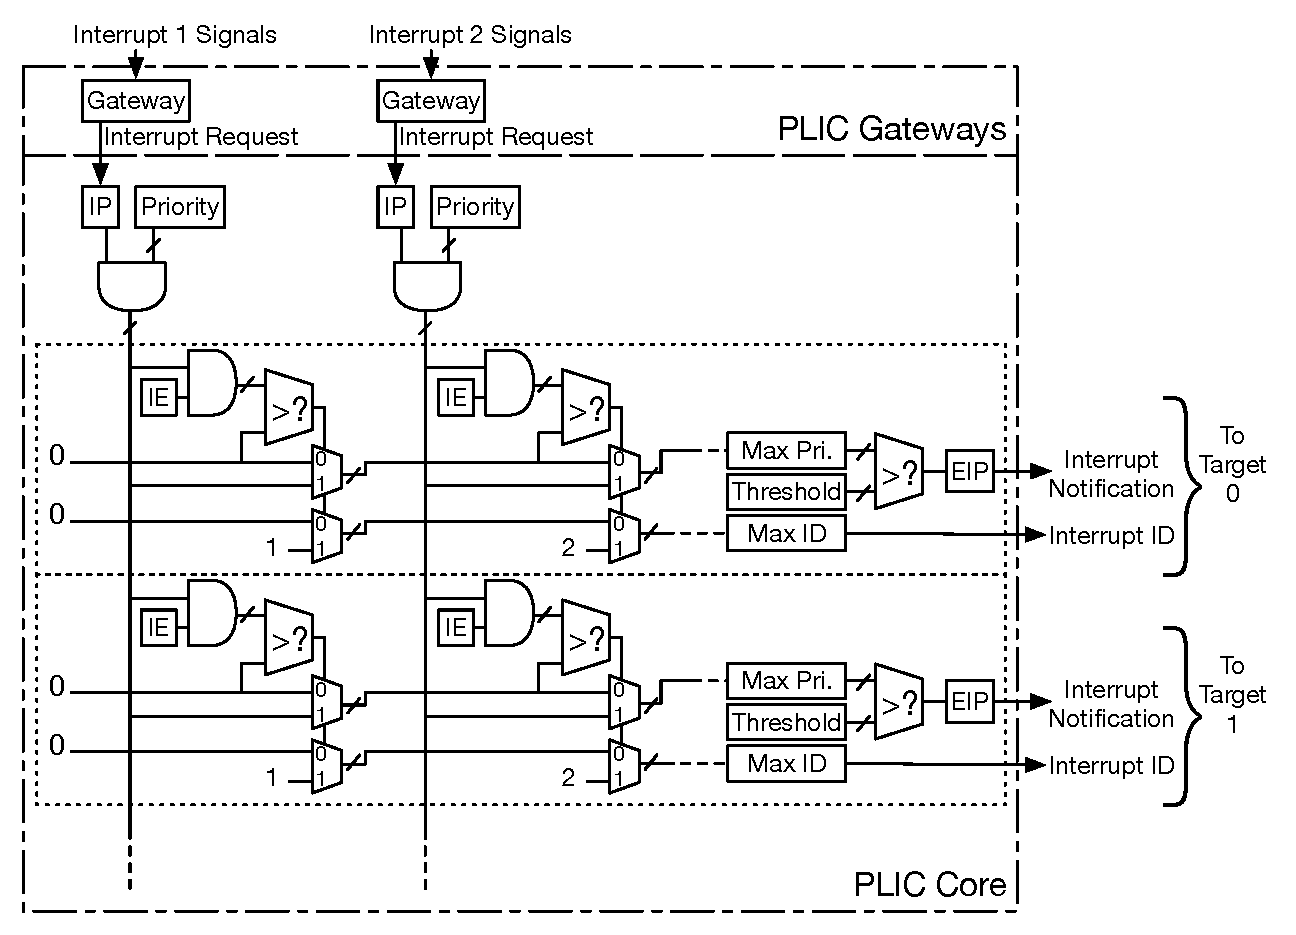
\includegraphics[width=\textwidth]{figs/PLIC-block-diagram.pdf}
\caption{Platform-Level Interrupt Controller (PLIC) conceptual block
  diagram.  The figure shows the first two of potentially many
  interrupt sources, and the first two of potentially many interrupt
  targets.  The figure is just intended to show the logic of the
  PLIC's operation, not to represent a realistic implementation
  strategy.}
\label{fig:plic}
\end{figure}

\section{Interrupt Sources}

RISC-V harts can have both local and global interrupt sources.  Only
global interrupt sources are handled by the PLIC.

\subsection{Local Interrupt Sources}

Each hart has a number of {\em local interrupt sources} that do not
pass through the PLIC, including the standard software interrupts and
timer interrupts for each privilege level.  Local interrupts can be
serviced quickly since there will be minimal latency between the
source and the servicing hart, no arbitration is required to determine
which hart will service the request, and the servicing hart can
quickly determine the interrupt source using the {\tt mcause}
register.

All local interrupts follow a level-based model, where an interrupt is
pending if the corresponding bit in {\tt mip} is set.  The interrupt
handler must clear the hardware condition that is causing the {\tt
  mip} bit to be set to avoid retaking the interrupt after re-enabling
interrupts on exit from the interrupt handler.

Additional non-standard local interrupt sources can be made visible to
machine-mode by adding them to the high bits of the {\tt mip}/{\tt
  mie} registers, with corresponding additional cause values returned
in the {\tt mcause} register.  These additional non-standard local
interrupts may also be made visible to lower privilege levels, using
the corresponding bits in the {\tt mideleg} register.  The priority of
non-standard local interrupt sources relative to external, timer, and
software interrupts is platform-specific.

\subsection{Global Interrupt Sources}

{\em Global interrupt sources} are those that are prioritized and
distributed by the PLIC.  Depending on the platform-specific PLIC
implementation, any global interrupt source could be routed to any
hart context.

Global interrupt sources can take many forms, including
level-triggered, edge-triggered, and message-signalled.  Some sources
might queue up a number of interrupt requests.  All global interrupt
sources are converted to a common interrupt request format for the
PLIC.

\section{Interrupt Targets and Hart Contexts}

Interrupt targets are usually hart contexts, where a hart context is a
given privilege mode on a given hart (though there are other possible
interrupt targets, such as DMA engines).  Not all hart contexts need
be interrupt targets, in particular, if a processor core does not
support delegating external interrupts to lower-privilege modes, then
the lower-privilege hart contexts will not be interrupt targets.
Interrupt notifications generated by the PLIC appear in the {\tt
  meip}/{\tt seip}/{\tt ueip} bits of the {\tt mip}/{\tt sip}/{\tt
  uip} registers for M/S/U modes, respectively.  For the notifications
to appear in lower-privilege {\em x}{\tt ip} registers, the corresponding
external interrupts must have been delegated in the higher-privilege
{\em y}{\tt ideleg} registers.

Each processor core must define a policy on how simultaneous active
interrupts are taken by multiple hart contexts on the core. For the
simple case of a single stack of hart contexts, one for each supported
privileged mode, interrupts for higher-privilege contexts can preempt
execution of interrupt handlers for lower-privilege contexts.  A
multithreaded processor core could run multiple independent interrupt
handlers on different hart contexts at the same time.  A processor
core could also provide hart contexts that are only used for interrupt
handling to reduce interrupt service latency, and these might preempt
interrupt handlers for other harts on the same core.

The PLIC treats each interrupt target independently and does not take
into account any interrupt prioritization scheme used by a component
that contains multiple interrupt targets.  As a result, the PLIC
provides no concept of interrupt preemption or nesting so this must be
handled by the cores hosting multiple interrupt target contexts.

\section{Interrupt Gateways}

The interrupt gateways are responsible for converting global interrupt
signals into a common interrupt request format, and for controlling
the flow of interrupt requests to the PLIC core.  At most one
interrupt request per interrupt source can be pending in the PLIC core
at any time, indicated by setting the source's IP bit.  The gateway
only forwards a new interrupt request to the PLIC core after receiving
notification that the interrupt handler servicing the previous
interrupt request from the same source has completed.

If the global interrupt source uses level-sensitive interrupts, the
gateway will convert the first assertion of the interrupt level into
an interrupt request, but thereafter the gateway will not forward an
additional interrupt request until it receives an interrupt completion
message.  On receiving an interrupt completion message, if the
interrupt is level-triggered and the interrupt is still asserted, a
new interrupt request will be forwarded to the PLIC core.  The gateway
does not have the facility to retract an interrupt request once
forwarded to the PLIC core.  If a level-sensitive interrupt source
deasserts the interrupt after the PLIC core accepts the request and
before the interrupt is serviced, the interrupt request remains
present in the IP bit of the PLIC core and will be serviced by a
handler, which will then have to determine that the interrupt device
no longer requires service.

If the global interrupt source was edge-triggered, the gateway will
convert the first matching signal edge into an interrupt request.
Depending on the design of the device and the interrupt handler,
between sending an interrupt request and receiving notice of its
handler's completion, the gateway might either ignore additional
matching edges or increment a counter of pending interrupts.  In
either case, the next interrupt request will not be forwarded to the
PLIC core until the previous completion message has been received.  If
the gateway has a pending interrupt counter, the counter will be
decremented when the interrupt request is accepted by the PLIC core.

Unlike dedicated-wire interrupt signals, message-signalled interrupts
(MSIs) are sent over the system interconnect via a message packet that
describes which interrupt is being asserted.  The message is decoded
to select an interrupt gateway, and the relevant gateway then handles
the MSI similar to an edge-triggered interrupt.

\section{Interrupt Identifiers (IDs)}

Global interrupt sources are assigned small unsigned integer
identifiers, beginning at the value 1.  An interrupt ID of 0 is
reserved to mean ``no interrupt''.

Interrupt identifiers are also used to break ties when two or more
interrupt sources have the same assigned priority.  Smaller values of
interrupt ID take precedence over larger values of interrupt ID.

\section{Interrupt Priorities}

Interrupt priorities are small unsigned integers, with a
platform-specific maximum number of supported levels.  The priority
value 0 is reserved to mean ``never interrupt'', and interrupt
priority increases with increasing integer values.

Each global interrupt source has an associated interrupt priority held
in a platform-specific memory-mapped register.  Different interrupt
sources need not support the same set of priority values.  A valid
implementation can hardwire all input priority levels.  Interrupt
source priority registers should be \warl\ fields to allow software to
determine the number and position of read-write bits in each priority
specification, if any.  To simplify discovery of supported priority
values, each priority register must support any combination of values
in the bits that are variable within the register, i.e., if there are
two variable bits in the register, all four combinations of values in
those bits must operate as valid priority levels.

\begin{commentary}
 In the degenerate case, all priorities can be hardwired to the value
 1, in which case input priorities are effectively determined by
 interrupt ID.

 The supported priority values can be determined as follows: 1) write
 all zeros to the priority register then 2) read back the value.  Any
 set bits are hardwired to 1.  Next, 3) write all ones to the
 register, and 4) read back the value.  Any clear bits are hardwired
 to 0.  Any set bits that were not found to be hardwired in step 2 are
 variable.  The supported priority levels are the set of values
 obtained by substituting all combinations of ones and zeros in the
 variable bits within the priority field.
\end{commentary}

\section{Interrupt Enables}

Each target has a vector of interrupt enable (IE) bits, one per
interrupt source.  The target will not receive interrupts from sources
that are disabled.  The IE bits for a single target should be packed
together as a bit vector in platform-specific memory-mapped control
registers to support rapid context switching of the IE bits for a
target.  IE bits are \warl\ fields that can be hardwired to either 0
or 1.

\begin{commentary}
A large number of potential IE bits might be hardwired to zero in
cases where some interrupt sources can only be routed to
a subset of targets.

A larger number of bits might be wired to 1 for an embedded device
with fixed interrupt routing.  Interrupt priorities, thresholds, and
hart-internal interrupt masking provide considerable flexibility in
ignoring external interrupts even if a global interrupt source is
always enabled.
\end{commentary}

\section{Interrupt Priority Thresholds}

Each interrupt target has an associated priority threshold, held in a
platform-specific memory-mapped register.  Only active interrupts that
have a priority strictly greater than the threshold will cause a
interrupt notification to be sent to the target.  Different interrupt
targets need not support the same set of priority threshold values.
Interrupt target threshold registers should be \warl\ fields to allow
software to determine the supported thresholds.  A threshold register
should always be able to hold the value zero, in which case, no
interrupts are masked.  If implemented, the threshold register will
usually also be able to hold the maximum priority level, in which case
all interrupts are masked.

\begin{commentary}
A simple valid implementation is to hardwire the threshold to zero, in
which case it has no effect, and the individual enable bits will have
to be saved and restored to attain the same effect.  While the
function of the threshold can be achieved by changing the
interrupt-enable bits, manipulating a single threshold value avoids
the target having to consider the individual priority levels of each
interrupt source, and saving and restoring all the interrupt enables.
Changing the threshold quickly might be especially important for
systems that move frequently between power states.
\end{commentary}

\section{Interrupt Notifications}

Each interrupt target has an {\em external interrupt pending} (EIP)
bit in the PLIC core that indicates that the corresponding target has
a pending interrupt waiting for service.  The value in EIP can change
as a result of changes to state in the PLIC core, brought on by
interrupt sources, interrupt targets, or other agents manipulating
register values in the PLIC.  The value in EIP is communicated to the
destination target as an interrupt notification.  If the target is a
RISC-V hart context, the interrupt notifications arrive on the {\tt
  meip}/{\tt seip}/{\tt ueip} bits depending on the
privilege level of the hart context.

\begin{commentary}
In simple systems, the interrupt notifications will be simple wires
connected to the processor implementing a hart.  In more complex
platforms, the notifications might be routed as messages across a
system interconnect.
\end{commentary}

The PLIC hardware only supports multicasting of interrupts, such that
all enabled targets will receive interrupt notifications for a given
active interrupt.

\begin{commentary}
Multicasting provides rapid response since the fastest responder
claims the interrupt, but can be wasteful in high-interrupt-rate
scenarios if multiple harts take a trap for an interrupt that only one
can successfully claim.  Software can modulate the PLIC IE bits as
part of each interrupt handler to provide alternate policies, such as
interrupt affinity or round-robin unicasting.
\end{commentary}

Depending on the platform architecture and the method used to
transport interrupt notifications, these might take some time to be
received at the targets.  The PLIC is guaranteed to eventually deliver
all state changes in EIP to all targets, provided there is no
intervening activity in the PLIC core.

\begin{commentary}
The value in an interrupt notification is only guaranteed to hold an
EIP value that was valid at some point in the past.  In particular, a
second target can respond and claim an interrupt while a notification
to the first target is still in flight, such that when the first
target tries to claim the interrupt it finds it has no active
interrupts in the PLIC core.
\end{commentary}

\section{Interrupt Claims}

Sometime after a target receives an interrupt notification, it might
decide to service the interrupt.  The target sends an {\em interrupt
  claim} message to the PLIC core, which will usually be implemented
as a non-idempotent memory-mapped I/O control register read.  On
receiving a claim message, the PLIC core will atomically determine the
ID of the highest-priority pending interrupt for the target and then
clear down the corresponding source's IP bit.  The PLIC core will then
return the ID to the target.  The PLIC core will return an ID of zero,
if there were no pending interrupts for the target when the claim was
serviced.

After the highest-priority pending interrupt is claimed by a target
and the corresponding IP bit is cleared, other lower-priority pending
interrupts might then become visible to the target, and so the PLIC
EIP bit might not be cleared after a claim.  The interrupt handler
can check the local {\tt meip}/{\tt seip}/{\tt ueip} bits
before exiting the handler, to allow more efficient service of other
interrupts without first restoring the interrupted context and taking
another interrupt trap.

It is always legal for a hart to perform a claim even if the EIP is
not set.  In particular, a hart could set the threshold value to maximum
to disable interrupt notifications and instead poll for active
interrupts using periodic claim requests, though a simpler approach to
implement polling would be to clear the external interrupt enable in
the corresponding {\em x}{\tt ie} register for privilege mode {\em x}.

\section{Interrupt Completion}

After a handler has completed service of an interrupt, the associated
gateway must be sent an interrupt completion message, usually as a
write to a non-idempotent memory-mapped I/O control register.  The
gateway will only forward additional interrupts to the PLIC core after
receiving the completion message.

\section{Interrupt Flow}

Figure~\ref{fig:intflow} shows the messages flowing between agents
when handling interrupts via the PLIC.

\begin{figure}[hb!]
\centering
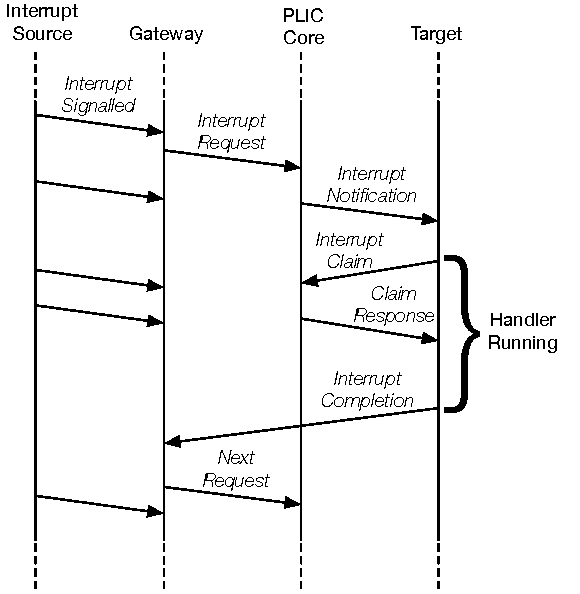
\includegraphics[width=4.0in]{figs/PLIC-interrupt-flow.pdf}
\caption{ Flow of interrupt processing via the PLIC.}
\label{fig:intflow}
\end{figure}

The gateway will only forward a single interrupt request at a time to
the PLIC, and not forward subsequent interrupts requests until an
interrupt completion is received.  The PLIC will set the IP bit once
it accepts an interrupt request from the gateway, and sometime later
forward an interrupt notification to the target.  The target might
take a while to respond to a new interrupt arriving, but will then
send an interrupt claim request to the PLIC core to obtain the
interrupt ID.  The PLIC core will atomically return the ID and clear
the corresponding IP bit, after which no other target can claim the
same interrupt request.  Once the handler has processed the interrupt,
it sends an interrupt completion message to the gateway to allow a new
interrupt request.

\section{PLIC Core Specification}

The operation of the PLIC core can be specified as a non-deterministic
finite-state machine with input and output message queues, with the
following atomic actions:

\begin{itemize}

\item {\bf Write Register: } A message containing a register write
  request is dequeued.  One of the internal registers is written,
  where an internal register can be a priority, an interrupt-enable
  (IE), or a threshold.

\item {\bf Accept Request: } If the IP bit corresponding to the
  interrupt source is clear, a message containing an interrupt request
  from a gateway is dequeued and the IP bit is set.

\item {\bf Process Claim: } An interrupt claim message is dequeued.  A
  claim-response message is enqueued to the requester with the ID of
  the highest-priority active interrupt for that target, and the IP
  bit corresponding to this interrupt source is cleared.

\end{itemize}

The value in the EIP bit is determined as a combinational function of
the PLIC Core state.  Interrupt notifications are sent via an
autonomous process that ensures the EIP value is eventually reflected
at the target. 

Note that the operation of the interrupt gateways is decoupled from
the PLIC core.  A gateway can handle parsing of interrupt signals and
processing interrupt completion messages concurrently with other
operations in the PLIC core.

\begin{commentary}
Figure~\ref{fig:plic} is a high-level conceptual view of the PLIC
design.  The PLIC core can be implemented in many ways provided its
behavior can always be understood as following from some sequential
ordering of these atomic actions.  In particular, the PLIC might
process multiple actions in a single clock cycle, or might process
each action over many clock cycles.
\end{commentary}

\section{Controlling Access to the PLIC}

In the expected use case, only machine mode accesses the source
priority, source pending, and target interrupt enables to configure
the interrupt subsystem.  Lower-privilege modes access these features
via ABI or SBI calls. The interrupt enables act as a protection
mechanism where a target can only signal completion to an interrupt
gateway that is currently enabled for that target.

Interrupt handlers that run with lower than machine-mode privilege
need only be able to perform a claim read and a completion write, and
to set their target threshold value.  The memory map for these
registers should allow machine mode to protect different targets from
each other's accesses, using either physical memory protection or
virtual memory page protections.


\chapter{Machine Configuration Description}
\label{cfgstr}

\begin{commentary}
  To reduce porting effort for OS boots, we have reverted back to
  using Device Trees to communicate platform information to the
  kernel, so this chapter is out of date.  Config string was designed
  for other uses in addition, but for now, we are staying with a
  standard device tree model.
 \end{commentary}

RISC-V platforms may contain myriad devices, processor cores, and
configuration parameters.  To support higher-level software, including
bootloaders and operating systems, it is recommended that hardware
platforms embed a description of their components in read-only memory
that is directly accessible after processor reset for use by low-level
system software, external debuggers, or manufacturing test procedures.
We call this low-level embedded information a configuration
description.  We define here a standard mechanism to encode and locate
the configuration information, and to determine the format of the
configuration information.

\section{Configuration String Search Procedure}

The platform must describe how to locate a pointer to find this
string, for example, by specifying a fixed physical address at which
the pointer resides.  To support a wide variety of platforms,
configuration formats, and chips with manufacturing-time programming
of configuration options, a flexible search procedure is defined to
locate the configuration information seeded by the initial pointer
specified by the platform.

The configuration string pointer provided by the platform points to an
initial memory address at which the search for configuration string
begins.

The configuration string cannot begin with a padding byte, where a
padding byte is defined to contain either {\tt 0x0} or {\tt 0xff}, but
can be preceded by up to 63 padding bytes that are ignored.  If 64
padding bytes are encountered, then the search terminates without
finding a config string.

\begin{commentary}
The padding bytes represent common values returned by unpopulated
memory or bus regions or unprogrammed non-volatile
memory. Configuration strings can therefore include pointers to
regions that are optionally populated or programmed, and these regions
will be ignored if there is nothing present.  The padding bytes also
support alignment of binary data structures.
\end{commentary}

Otherwise the first non-padding byte is the beginning of the
configuration information.  For example, configuration information in
Device Tree String format would begin with a ``/dts-v1/''.
Configuration information in Flattened Device Tree format would begin
with the magic number {\tt 0xd00dfeed}.  Configuration information in
the config string format would begin with ``/cs-v1/''.
\begin{commentary}
  Config string is a new format that is backwards-compatible with
  device tree string (as far as DTS specs exist) but can include
  additional configuration information in other memory regions.
\end{commentary}


\chapter{Supervisor Binary Interface (SBI)}

This chapter is a placeholder to describe the form of the SBIs we're
envisioning for the RISC-V supervisor.

The SBI captures the instructions that can be executed together with a
set of SBI calls out to the supervisor execution environment (SEE) on
a given platform.

Several features that might normally handled by the supervisor
operating system (OS) directly are handled via SBI calls to the SEE in
RISC-V, including:

\begin{itemize}

\item Reset is handled by the SEE and once the machine is set up, the
  OS kernel is mapped into virtual memory, and its entry point is called.

\item Machine-check errors and other non-maskable interrupts are
  handled by the SEE before vectoring into the OS if recovery is
  possible.

\item Some device drivers may be handled by the SEE, and managed via
  virtual device calls over the SBI.

\item The presence and version of supported instruction-set extensions
  is obtained via an SBI call to return the configuration string
  rather than a machine register.  This allows for an arbitrarily
  large definition of instruction-set extensions, and simplifies
  virtualization where the returned machine configuration might be
  modified to emulate different architectures on a given hardware
  platform.

\end{itemize}

The SBI employs the same calling convention as the ABI specified in Volume
I of this manual.  SBI entry points are located in the uppermost
\wunits{2}{KiB} of the virtual address space, so that they may be invoked with
a single {\tt jalr} instruction with {\tt x0} as the base register.

Table~\ref{sbicalls} gives a preliminary list of SBI calls.

\begin{table*}[h!]
\begin{center}
\begin{tabular}{| >{\ttfamily\catcode`_=12}l|p{8cm}|}
\hline
const char* sbi_get_config(void); & \parbox{8cm}{Get pointer to
  configuration string.}\\ \hline
size_t sbi_hart_id(void); & \parbox{8cm}{Get ID of current hart, in
  range \\ {\tt [0, number\_harts - 1 ]}.} \\ \hline
int sbi_send_ipi(size_t hart_id); & Send an interprocessor interrupt; returns 0 on success or -1 if hart ID is invalid. \\ \hline
bool sbi_clear_ipi(void); & Clear local interprocessor interrupt. Returns 1 if an IPI was pending, else 0. \\ \hline
void sbi_shutdown(void); & Terminate this supervisor-mode process. \\ \hline
int sbi_console_putchar(uint8_t ch); & Write byte to debug console (blocking); returns 0 on success, else -1. \\ \hline
int sbi_console_getchar(void); & Read byte from debug console; returns the byte on success, or -1 for failure. \\ \hline

& \multirow{4}{*}{\parbox{8cm}{Instruct other harts to execute SFENCE.VMA.  {\tt harts} points to a bitmask of remote hart IDs; NULL indicates all harts.  {\tt asid} holds the address-space ID; 0 indicates all address spaces.}} \\
void sbi_remote_sfence_vm( & \\
\ \ const uintptr_t* harts, size_t asid); & \\
& \\ \hline

void sbi_remote_sfence_vm_range(
& \multirow{3}{*}{\parbox{8cm}{Like {\tt sbi\_remote\_sfence\_vm}, but only orders updates to leaf page tables mapping the range {\tt [start, start+size-1]}.}} \\
\ \ const uintptr_t* harts, size_t asid, & \\
\ \ uintptr_t start, uintptr_t size); & \\ \hline

void sbi_remote_fence_i(
& \multirow{2}{*}{\parbox{8cm}{Instruct remote harts to execute FENCE.I.  {\tt harts} is as with {\tt sbi\_remote\_sfence\_vm}.}} \\
\ \ const uintptr_t* harts); & \\ \hline

int sbi_mask_interrupt(int which); & Disable a PLIC interrupt line. Returns 0 if previously disabled, 1 if previously enabled, or -1 if {\tt which} is invalid. \\ \hline
int sbi_unmask_interrupt(int which); & Enable a PLIC interrupt line. Return value is as with {\tt sbi\_mask\_interrupt}. \\ \hline
\end{tabular}
\end{center}
\caption{SBI calls.}
\label{sbicalls}
\end{table*}

\chapter{History}

\section*{Acknowledgments}

Thanks to Jacob Bachmeyer,
Allen J. Baum, Ruslan Bukin, Christopher Celio, David
Chisnall, Palmer Dabbelt, Monte Dalrymple, Dennis Ferguson, Mike
Frysinger, John Hauser, Jonathan Neusch{\"a}fer, Rishiyur Nikhil, Stefan O'Rear,
Albert Ou, John Ousterhout, Colin Schmidt, Wesley Terpstra, Matt
Thomas, Tommy Thorn, Ray VanDeWalker, and Reinoud Zandijk for feedback
on the privileged specification.

\section{Funding}

Development of the RISC-V architecture and implementations has been
partially funded by the following sponsors.
\begin{itemize}
\item {\bf Par Lab:} Research supported by Microsoft (Award \#024263)
  and Intel (Award \#024894) funding and by matching funding by
  U.C. Discovery (Award \#DIG07-10227). Additional support came from
  Par Lab affiliates Nokia, NVIDIA, Oracle, and Samsung.

\item {\bf Project Isis:} DoE Award DE-SC0003624.

\item {\bf ASPIRE Lab}: DARPA PERFECT program, Award HR0011-12-2-0016.
  DARPA POEM program Award HR0011-11-C-0100.  The Center for Future
  Architectures Research (C-FAR), a STARnet center funded by the
  Semiconductor Research Corporation.  Additional support from ASPIRE
  industrial sponsor, Intel, and ASPIRE affiliates, Google, Huawei,
  Nokia, NVIDIA, Oracle, and Samsung.
\end{itemize}

The content of this paper does not necessarily reflect the position or the
policy of the US government and no official endorsement should be
inferred. 


\bibliographystyle{plain}
\bibliography{riscv-spec}

\end{document}
